\documentclass[twoside]{book}

% Packages required by doxygen
\usepackage{fixltx2e}
\usepackage{calc}
\usepackage{doxygen}
\usepackage[export]{adjustbox} % also loads graphicx
\usepackage{graphicx}
\usepackage[utf8]{inputenc}
\usepackage{makeidx}
\usepackage{multicol}
\usepackage{multirow}
\PassOptionsToPackage{warn}{textcomp}
\usepackage{textcomp}
\usepackage[nointegrals]{wasysym}
\usepackage[table]{xcolor}

% Font selection
\usepackage[T1]{fontenc}
\usepackage[scaled=.90]{helvet}
\usepackage{courier}
\usepackage{amssymb}
\usepackage{sectsty}
\renewcommand{\familydefault}{\sfdefault}
\allsectionsfont{%
  \fontseries{bc}\selectfont%
  \color{darkgray}%
}
\renewcommand{\DoxyLabelFont}{%
  \fontseries{bc}\selectfont%
  \color{darkgray}%
}
\newcommand{\+}{\discretionary{\mbox{\scriptsize$\hookleftarrow$}}{}{}}

% Page & text layout
\usepackage{geometry}
\geometry{%
  a4paper,%
  top=2.5cm,%
  bottom=2.5cm,%
  left=2.5cm,%
  right=2.5cm%
}
\tolerance=750
\hfuzz=15pt
\hbadness=750
\setlength{\emergencystretch}{15pt}
\setlength{\parindent}{0cm}
\setlength{\parskip}{3ex plus 2ex minus 2ex}
\makeatletter
\renewcommand{\paragraph}{%
  \@startsection{paragraph}{4}{0ex}{-1.0ex}{1.0ex}{%
    \normalfont\normalsize\bfseries\SS@parafont%
  }%
}
\renewcommand{\subparagraph}{%
  \@startsection{subparagraph}{5}{0ex}{-1.0ex}{1.0ex}{%
    \normalfont\normalsize\bfseries\SS@subparafont%
  }%
}
\makeatother

% Headers & footers
\usepackage{fancyhdr}
\pagestyle{fancyplain}
\fancyhead[LE]{\fancyplain{}{\bfseries\thepage}}
\fancyhead[CE]{\fancyplain{}{}}
\fancyhead[RE]{\fancyplain{}{\bfseries\leftmark}}
\fancyhead[LO]{\fancyplain{}{\bfseries\rightmark}}
\fancyhead[CO]{\fancyplain{}{}}
\fancyhead[RO]{\fancyplain{}{\bfseries\thepage}}
\fancyfoot[LE]{\fancyplain{}{}}
\fancyfoot[CE]{\fancyplain{}{}}
\fancyfoot[RE]{\fancyplain{}{\bfseries\scriptsize Generated by Doxygen }}
\fancyfoot[LO]{\fancyplain{}{\bfseries\scriptsize Generated by Doxygen }}
\fancyfoot[CO]{\fancyplain{}{}}
\fancyfoot[RO]{\fancyplain{}{}}
\renewcommand{\footrulewidth}{0.4pt}
\renewcommand{\chaptermark}[1]{%
  \markboth{#1}{}%
}
\renewcommand{\sectionmark}[1]{%
  \markright{\thesection\ #1}%
}

% Indices & bibliography
\usepackage{natbib}
\usepackage[titles]{tocloft}
\setcounter{tocdepth}{3}
\setcounter{secnumdepth}{5}
\makeindex

% Hyperlinks (required, but should be loaded last)
\usepackage{ifpdf}
\ifpdf
  \usepackage[pdftex,pagebackref=true]{hyperref}
\else
  \usepackage[ps2pdf,pagebackref=true]{hyperref}
\fi
\hypersetup{%
  colorlinks=true,%
  linkcolor=blue,%
  citecolor=blue,%
  unicode%
}

% Custom commands
\newcommand{\clearemptydoublepage}{%
  \newpage{\pagestyle{empty}\cleardoublepage}%
}

\usepackage{caption}
\captionsetup{labelsep=space,justification=centering,font={bf},singlelinecheck=off,skip=4pt,position=top}

%===== C O N T E N T S =====

\begin{document}

% Titlepage & ToC
\hypersetup{pageanchor=false,
             bookmarksnumbered=true,
             pdfencoding=unicode
            }
\pagenumbering{alph}
\begin{titlepage}
\vspace*{7cm}
\begin{center}%
{\Large Flow \\[1ex]\large 1.\+0.\+0 }\\
\vspace*{1cm}
{\large Generated by Doxygen 1.8.13}\\
\end{center}
\end{titlepage}
\clearemptydoublepage
\pagenumbering{roman}
\tableofcontents
\clearemptydoublepage
\pagenumbering{arabic}
\hypersetup{pageanchor=true}

%--- Begin generated contents ---
\chapter{Flow}
\label{index}\hypertarget{index}{}C++14, header-\/only library for multi-\/stream data synchronization.

\subsection*{What is this used for?}

This library is meant for generating groups of data from separate series. The core problems it is meant to address are\+:


\begin{DoxyItemize}
\item How do we know what elements of data across multiple input streams relate to one other?
\item How do we know when this data is ready to be retrieved (\char`\"{}captured\char`\"{}) for further use?
\item How do we capture different types of data uniformly and with minimal overhead?
\end{DoxyItemize}

In addressing these problems, this library enables data-\/driven event execution using data collected from distinct streaming series.

\subsubsection*{Example use case}

At Fetch Robotics Inc., this library is used in tandem with R\+OS. R\+OS subscribers are used to feed data into {\ttfamily Flow} capture buffers with light message feeding callbacks. The callbacks transfer R\+OS messages into the appropriate {\ttfamily Flow} capture buffer. {\ttfamily Flow} entities are serviced separately to compute events from these messages. The resulting data frames from synchronization contain all messages needed to run a particular task. In this way, messages are also used as a pace-\/setting mechanism for core execution blocks. 
\chapter{Namespace Index}
\section{Namespace List}
Here is a list of all documented namespaces with brief descriptions\+:\begin{DoxyCompactList}
\item\contentsline{section}{\hyperlink{namespaceflow}{flow} \\*Flow input synchronization library components }{\pageref{namespaceflow}}{}
\item\contentsline{section}{\hyperlink{namespaceflow_1_1driver}{flow\+::driver} \\*Synchronizations buffer with policies which produce sequencing ranges }{\pageref{namespaceflow_1_1driver}}{}
\item\contentsline{section}{\hyperlink{namespaceflow_1_1follower}{flow\+::follower} \\*Synchronization buffers with sequencing range-\/dependent policies }{\pageref{namespaceflow_1_1follower}}{}
\end{DoxyCompactList}

\chapter{Hierarchical Index}
\section{Class Hierarchy}
This inheritance list is sorted roughly, but not completely, alphabetically\+:\begin{DoxyCompactList}
\item \contentsline{section}{flow\+:\+:Captor\+Interface$<$ CaptorT $>$}{\pageref{classflow_1_1_captor_interface}}{}
\item \contentsline{section}{flow\+:\+:Captor\+Interface$<$ Captor$<$ CaptorT, LockableT, Queue\+MonitorT $>$ $>$}{\pageref{classflow_1_1_captor_interface}}{}
\begin{DoxyCompactList}
\item \contentsline{section}{flow\+:\+:Captor$<$ CaptorT, LockableT, Queue\+MonitorT $>$}{\pageref{classflow_1_1_captor}}{}
\end{DoxyCompactList}
\item \contentsline{section}{flow\+:\+:Captor\+Interface$<$ Captor$<$ Driver$<$ Batch$<$ DispatchT, Lock\+PolicyT, ContainerT, Queue\+MonitorT $>$ $>$, Captor\+Traits$<$ Batch$<$ DispatchT, Lock\+PolicyT, ContainerT, Queue\+MonitorT $>$ $>$\+:\+:Lock\+Policy\+Type, Default\+Dispatch\+Queue\+Monitor $>$ $>$}{\pageref{classflow_1_1_captor_interface}}{}
\begin{DoxyCompactList}
\item \contentsline{section}{flow\+:\+:Captor$<$ Driver$<$ Batch$<$ DispatchT, Lock\+PolicyT, ContainerT, Queue\+MonitorT $>$ $>$, Captor\+Traits$<$ Batch$<$ DispatchT, Lock\+PolicyT, ContainerT, Queue\+MonitorT $>$ $>$\+:\+:Lock\+Policy\+Type, Default\+Dispatch\+Queue\+Monitor $>$}{\pageref{classflow_1_1_captor}}{}
\begin{DoxyCompactList}
\item \contentsline{section}{flow\+:\+:Driver$<$ Batch$<$ DispatchT, Lock\+PolicyT, ContainerT, Queue\+MonitorT $>$ $>$}{\pageref{classflow_1_1_driver}}{}
\begin{DoxyCompactList}
\item \contentsline{section}{flow\+:\+:driver\+:\+:Batch$<$ DispatchT, Lock\+PolicyT, ContainerT, Queue\+MonitorT $>$}{\pageref{classflow_1_1driver_1_1_batch}}{}
\end{DoxyCompactList}
\end{DoxyCompactList}
\end{DoxyCompactList}
\item \contentsline{section}{flow\+:\+:Captor\+Interface$<$ Captor$<$ Driver$<$ Chunk$<$ DispatchT, Lock\+PolicyT, ContainerT, Queue\+MonitorT $>$ $>$, Captor\+Traits$<$ Chunk$<$ DispatchT, Lock\+PolicyT, ContainerT, Queue\+MonitorT $>$ $>$\+:\+:Lock\+Policy\+Type, Default\+Dispatch\+Queue\+Monitor $>$ $>$}{\pageref{classflow_1_1_captor_interface}}{}
\begin{DoxyCompactList}
\item \contentsline{section}{flow\+:\+:Captor$<$ Driver$<$ Chunk$<$ DispatchT, Lock\+PolicyT, ContainerT, Queue\+MonitorT $>$ $>$, Captor\+Traits$<$ Chunk$<$ DispatchT, Lock\+PolicyT, ContainerT, Queue\+MonitorT $>$ $>$\+:\+:Lock\+Policy\+Type, Default\+Dispatch\+Queue\+Monitor $>$}{\pageref{classflow_1_1_captor}}{}
\begin{DoxyCompactList}
\item \contentsline{section}{flow\+:\+:Driver$<$ Chunk$<$ DispatchT, Lock\+PolicyT, ContainerT, Queue\+MonitorT $>$ $>$}{\pageref{classflow_1_1_driver}}{}
\begin{DoxyCompactList}
\item \contentsline{section}{flow\+:\+:driver\+:\+:Chunk$<$ DispatchT, Lock\+PolicyT, ContainerT, Queue\+MonitorT $>$}{\pageref{classflow_1_1driver_1_1_chunk}}{}
\end{DoxyCompactList}
\end{DoxyCompactList}
\end{DoxyCompactList}
\item \contentsline{section}{flow\+:\+:Captor\+Interface$<$ Captor$<$ Driver$<$ Next$<$ DispatchT, Lock\+PolicyT, ContainerT, Queue\+MonitorT $>$ $>$, Captor\+Traits$<$ Next$<$ DispatchT, Lock\+PolicyT, ContainerT, Queue\+MonitorT $>$ $>$\+:\+:Lock\+Policy\+Type, Default\+Dispatch\+Queue\+Monitor $>$ $>$}{\pageref{classflow_1_1_captor_interface}}{}
\begin{DoxyCompactList}
\item \contentsline{section}{flow\+:\+:Captor$<$ Driver$<$ Next$<$ DispatchT, Lock\+PolicyT, ContainerT, Queue\+MonitorT $>$ $>$, Captor\+Traits$<$ Next$<$ DispatchT, Lock\+PolicyT, ContainerT, Queue\+MonitorT $>$ $>$\+:\+:Lock\+Policy\+Type, Default\+Dispatch\+Queue\+Monitor $>$}{\pageref{classflow_1_1_captor}}{}
\begin{DoxyCompactList}
\item \contentsline{section}{flow\+:\+:Driver$<$ Next$<$ DispatchT, Lock\+PolicyT, ContainerT, Queue\+MonitorT $>$ $>$}{\pageref{classflow_1_1_driver}}{}
\begin{DoxyCompactList}
\item \contentsline{section}{flow\+:\+:driver\+:\+:Next$<$ DispatchT, Lock\+PolicyT, ContainerT, Queue\+MonitorT $>$}{\pageref{classflow_1_1driver_1_1_next}}{}
\end{DoxyCompactList}
\end{DoxyCompactList}
\end{DoxyCompactList}
\item \contentsline{section}{flow\+:\+:Captor\+Interface$<$ Captor$<$ Driver$<$ PolicyT $>$, Captor\+Traits$<$ PolicyT $>$\+:\+:Lock\+Policy\+Type, Default\+Dispatch\+Queue\+Monitor $>$ $>$}{\pageref{classflow_1_1_captor_interface}}{}
\begin{DoxyCompactList}
\item \contentsline{section}{flow\+:\+:Captor$<$ Driver$<$ PolicyT $>$, Captor\+Traits$<$ PolicyT $>$\+:\+:Lock\+Policy\+Type, Default\+Dispatch\+Queue\+Monitor $>$}{\pageref{classflow_1_1_captor}}{}
\begin{DoxyCompactList}
\item \contentsline{section}{flow\+:\+:Driver$<$ PolicyT $>$}{\pageref{classflow_1_1_driver}}{}
\end{DoxyCompactList}
\end{DoxyCompactList}
\item \contentsline{section}{flow\+:\+:Captor\+Interface$<$ Captor$<$ Driver$<$ Throttled$<$ DispatchT, Lock\+PolicyT, ContainerT, Queue\+MonitorT $>$ $>$, Captor\+Traits$<$ Throttled$<$ DispatchT, Lock\+PolicyT, ContainerT, Queue\+MonitorT $>$ $>$\+:\+:Lock\+Policy\+Type, Default\+Dispatch\+Queue\+Monitor $>$ $>$}{\pageref{classflow_1_1_captor_interface}}{}
\begin{DoxyCompactList}
\item \contentsline{section}{flow\+:\+:Captor$<$ Driver$<$ Throttled$<$ DispatchT, Lock\+PolicyT, ContainerT, Queue\+MonitorT $>$ $>$, Captor\+Traits$<$ Throttled$<$ DispatchT, Lock\+PolicyT, ContainerT, Queue\+MonitorT $>$ $>$\+:\+:Lock\+Policy\+Type, Default\+Dispatch\+Queue\+Monitor $>$}{\pageref{classflow_1_1_captor}}{}
\begin{DoxyCompactList}
\item \contentsline{section}{flow\+:\+:Driver$<$ Throttled$<$ DispatchT, Lock\+PolicyT, ContainerT, Queue\+MonitorT $>$ $>$}{\pageref{classflow_1_1_driver}}{}
\begin{DoxyCompactList}
\item \contentsline{section}{flow\+:\+:driver\+:\+:Throttled$<$ DispatchT, Lock\+PolicyT, ContainerT, Queue\+MonitorT $>$}{\pageref{classflow_1_1driver_1_1_throttled}}{}
\end{DoxyCompactList}
\end{DoxyCompactList}
\end{DoxyCompactList}
\item \contentsline{section}{flow\+:\+:Captor\+Interface$<$ Captor$<$ Follower$<$ Any\+Before$<$ DispatchT, Lock\+PolicyT, ContainerT, Queue\+MonitorT $>$ $>$, Captor\+Traits$<$ Any\+Before$<$ DispatchT, Lock\+PolicyT, ContainerT, Queue\+MonitorT $>$ $>$\+:\+:Lock\+Policy\+Type, Captor\+Traits$<$ Any\+Before$<$ DispatchT, Lock\+PolicyT, ContainerT, Queue\+MonitorT $>$ $>$\+:\+:Dispatch\+Queue\+Monitor\+Type $>$ $>$}{\pageref{classflow_1_1_captor_interface}}{}
\begin{DoxyCompactList}
\item \contentsline{section}{flow\+:\+:Captor$<$ Follower$<$ Any\+Before$<$ DispatchT, Lock\+PolicyT, ContainerT, Queue\+MonitorT $>$ $>$, Captor\+Traits$<$ Any\+Before$<$ DispatchT, Lock\+PolicyT, ContainerT, Queue\+MonitorT $>$ $>$\+:\+:Lock\+Policy\+Type, Captor\+Traits$<$ Any\+Before$<$ DispatchT, Lock\+PolicyT, ContainerT, Queue\+MonitorT $>$ $>$\+:\+:Dispatch\+Queue\+Monitor\+Type $>$}{\pageref{classflow_1_1_captor}}{}
\begin{DoxyCompactList}
\item \contentsline{section}{flow\+:\+:Follower$<$ Any\+Before$<$ DispatchT, Lock\+PolicyT, ContainerT, Queue\+MonitorT $>$ $>$}{\pageref{classflow_1_1_follower}}{}
\begin{DoxyCompactList}
\item \contentsline{section}{flow\+:\+:follower\+:\+:Any\+Before$<$ DispatchT, Lock\+PolicyT, ContainerT, Queue\+MonitorT $>$}{\pageref{classflow_1_1follower_1_1_any_before}}{}
\end{DoxyCompactList}
\end{DoxyCompactList}
\end{DoxyCompactList}
\item \contentsline{section}{flow\+:\+:Captor\+Interface$<$ Captor$<$ Follower$<$ Before$<$ DispatchT, Lock\+PolicyT, ContainerT, Queue\+MonitorT $>$ $>$, Captor\+Traits$<$ Before$<$ DispatchT, Lock\+PolicyT, ContainerT, Queue\+MonitorT $>$ $>$\+:\+:Lock\+Policy\+Type, Captor\+Traits$<$ Before$<$ DispatchT, Lock\+PolicyT, ContainerT, Queue\+MonitorT $>$ $>$\+:\+:Dispatch\+Queue\+Monitor\+Type $>$ $>$}{\pageref{classflow_1_1_captor_interface}}{}
\begin{DoxyCompactList}
\item \contentsline{section}{flow\+:\+:Captor$<$ Follower$<$ Before$<$ DispatchT, Lock\+PolicyT, ContainerT, Queue\+MonitorT $>$ $>$, Captor\+Traits$<$ Before$<$ DispatchT, Lock\+PolicyT, ContainerT, Queue\+MonitorT $>$ $>$\+:\+:Lock\+Policy\+Type, Captor\+Traits$<$ Before$<$ DispatchT, Lock\+PolicyT, ContainerT, Queue\+MonitorT $>$ $>$\+:\+:Dispatch\+Queue\+Monitor\+Type $>$}{\pageref{classflow_1_1_captor}}{}
\begin{DoxyCompactList}
\item \contentsline{section}{flow\+:\+:Follower$<$ Before$<$ DispatchT, Lock\+PolicyT, ContainerT, Queue\+MonitorT $>$ $>$}{\pageref{classflow_1_1_follower}}{}
\begin{DoxyCompactList}
\item \contentsline{section}{flow\+:\+:follower\+:\+:Before$<$ DispatchT, Lock\+PolicyT, ContainerT, Queue\+MonitorT $>$}{\pageref{classflow_1_1follower_1_1_before}}{}
\end{DoxyCompactList}
\end{DoxyCompactList}
\end{DoxyCompactList}
\item \contentsline{section}{flow\+:\+:Captor\+Interface$<$ Captor$<$ Follower$<$ Closest\+Before$<$ DispatchT, Lock\+PolicyT, ContainerT, Queue\+MonitorT $>$ $>$, Captor\+Traits$<$ Closest\+Before$<$ DispatchT, Lock\+PolicyT, ContainerT, Queue\+MonitorT $>$ $>$\+:\+:Lock\+Policy\+Type, Captor\+Traits$<$ Closest\+Before$<$ DispatchT, Lock\+PolicyT, ContainerT, Queue\+MonitorT $>$ $>$\+:\+:Dispatch\+Queue\+Monitor\+Type $>$ $>$}{\pageref{classflow_1_1_captor_interface}}{}
\begin{DoxyCompactList}
\item \contentsline{section}{flow\+:\+:Captor$<$ Follower$<$ Closest\+Before$<$ DispatchT, Lock\+PolicyT, ContainerT, Queue\+MonitorT $>$ $>$, Captor\+Traits$<$ Closest\+Before$<$ DispatchT, Lock\+PolicyT, ContainerT, Queue\+MonitorT $>$ $>$\+:\+:Lock\+Policy\+Type, Captor\+Traits$<$ Closest\+Before$<$ DispatchT, Lock\+PolicyT, ContainerT, Queue\+MonitorT $>$ $>$\+:\+:Dispatch\+Queue\+Monitor\+Type $>$}{\pageref{classflow_1_1_captor}}{}
\begin{DoxyCompactList}
\item \contentsline{section}{flow\+:\+:Follower$<$ Closest\+Before$<$ DispatchT, Lock\+PolicyT, ContainerT, Queue\+MonitorT $>$ $>$}{\pageref{classflow_1_1_follower}}{}
\begin{DoxyCompactList}
\item \contentsline{section}{flow\+:\+:follower\+:\+:Closest\+Before$<$ DispatchT, Lock\+PolicyT, ContainerT, Queue\+MonitorT $>$}{\pageref{classflow_1_1follower_1_1_closest_before}}{}
\end{DoxyCompactList}
\end{DoxyCompactList}
\end{DoxyCompactList}
\item \contentsline{section}{flow\+:\+:Captor\+Interface$<$ Captor$<$ Follower$<$ Count\+Before$<$ DispatchT, Lock\+PolicyT, ContainerT, Queue\+MonitorT $>$ $>$, Captor\+Traits$<$ Count\+Before$<$ DispatchT, Lock\+PolicyT, ContainerT, Queue\+MonitorT $>$ $>$\+:\+:Lock\+Policy\+Type, Captor\+Traits$<$ Count\+Before$<$ DispatchT, Lock\+PolicyT, ContainerT, Queue\+MonitorT $>$ $>$\+:\+:Dispatch\+Queue\+Monitor\+Type $>$ $>$}{\pageref{classflow_1_1_captor_interface}}{}
\begin{DoxyCompactList}
\item \contentsline{section}{flow\+:\+:Captor$<$ Follower$<$ Count\+Before$<$ DispatchT, Lock\+PolicyT, ContainerT, Queue\+MonitorT $>$ $>$, Captor\+Traits$<$ Count\+Before$<$ DispatchT, Lock\+PolicyT, ContainerT, Queue\+MonitorT $>$ $>$\+:\+:Lock\+Policy\+Type, Captor\+Traits$<$ Count\+Before$<$ DispatchT, Lock\+PolicyT, ContainerT, Queue\+MonitorT $>$ $>$\+:\+:Dispatch\+Queue\+Monitor\+Type $>$}{\pageref{classflow_1_1_captor}}{}
\begin{DoxyCompactList}
\item \contentsline{section}{flow\+:\+:Follower$<$ Count\+Before$<$ DispatchT, Lock\+PolicyT, ContainerT, Queue\+MonitorT $>$ $>$}{\pageref{classflow_1_1_follower}}{}
\begin{DoxyCompactList}
\item \contentsline{section}{flow\+:\+:follower\+:\+:Count\+Before$<$ DispatchT, Lock\+PolicyT, ContainerT, Queue\+MonitorT $>$}{\pageref{classflow_1_1follower_1_1_count_before}}{}
\end{DoxyCompactList}
\end{DoxyCompactList}
\end{DoxyCompactList}
\item \contentsline{section}{flow\+:\+:Captor\+Interface$<$ Captor$<$ Follower$<$ Latched$<$ DispatchT, Lock\+PolicyT, ContainerT, Queue\+MonitorT $>$ $>$, Captor\+Traits$<$ Latched$<$ DispatchT, Lock\+PolicyT, ContainerT, Queue\+MonitorT $>$ $>$\+:\+:Lock\+Policy\+Type, Captor\+Traits$<$ Latched$<$ DispatchT, Lock\+PolicyT, ContainerT, Queue\+MonitorT $>$ $>$\+:\+:Dispatch\+Queue\+Monitor\+Type $>$ $>$}{\pageref{classflow_1_1_captor_interface}}{}
\begin{DoxyCompactList}
\item \contentsline{section}{flow\+:\+:Captor$<$ Follower$<$ Latched$<$ DispatchT, Lock\+PolicyT, ContainerT, Queue\+MonitorT $>$ $>$, Captor\+Traits$<$ Latched$<$ DispatchT, Lock\+PolicyT, ContainerT, Queue\+MonitorT $>$ $>$\+:\+:Lock\+Policy\+Type, Captor\+Traits$<$ Latched$<$ DispatchT, Lock\+PolicyT, ContainerT, Queue\+MonitorT $>$ $>$\+:\+:Dispatch\+Queue\+Monitor\+Type $>$}{\pageref{classflow_1_1_captor}}{}
\begin{DoxyCompactList}
\item \contentsline{section}{flow\+:\+:Follower$<$ Latched$<$ DispatchT, Lock\+PolicyT, ContainerT, Queue\+MonitorT $>$ $>$}{\pageref{classflow_1_1_follower}}{}
\begin{DoxyCompactList}
\item \contentsline{section}{flow\+:\+:follower\+:\+:Latched$<$ DispatchT, Lock\+PolicyT, ContainerT, Queue\+MonitorT $>$}{\pageref{classflow_1_1follower_1_1_latched}}{}
\end{DoxyCompactList}
\end{DoxyCompactList}
\end{DoxyCompactList}
\item \contentsline{section}{flow\+:\+:Captor\+Interface$<$ Captor$<$ Follower$<$ Matched\+Stamp$<$ DispatchT, Lock\+PolicyT, ContainerT, Queue\+MonitorT $>$ $>$, Captor\+Traits$<$ Matched\+Stamp$<$ DispatchT, Lock\+PolicyT, ContainerT, Queue\+MonitorT $>$ $>$\+:\+:Lock\+Policy\+Type, Captor\+Traits$<$ Matched\+Stamp$<$ DispatchT, Lock\+PolicyT, ContainerT, Queue\+MonitorT $>$ $>$\+:\+:Dispatch\+Queue\+Monitor\+Type $>$ $>$}{\pageref{classflow_1_1_captor_interface}}{}
\begin{DoxyCompactList}
\item \contentsline{section}{flow\+:\+:Captor$<$ Follower$<$ Matched\+Stamp$<$ DispatchT, Lock\+PolicyT, ContainerT, Queue\+MonitorT $>$ $>$, Captor\+Traits$<$ Matched\+Stamp$<$ DispatchT, Lock\+PolicyT, ContainerT, Queue\+MonitorT $>$ $>$\+:\+:Lock\+Policy\+Type, Captor\+Traits$<$ Matched\+Stamp$<$ DispatchT, Lock\+PolicyT, ContainerT, Queue\+MonitorT $>$ $>$\+:\+:Dispatch\+Queue\+Monitor\+Type $>$}{\pageref{classflow_1_1_captor}}{}
\begin{DoxyCompactList}
\item \contentsline{section}{flow\+:\+:Follower$<$ Matched\+Stamp$<$ DispatchT, Lock\+PolicyT, ContainerT, Queue\+MonitorT $>$ $>$}{\pageref{classflow_1_1_follower}}{}
\begin{DoxyCompactList}
\item \contentsline{section}{flow\+:\+:follower\+:\+:Matched\+Stamp$<$ DispatchT, Lock\+PolicyT, ContainerT, Queue\+MonitorT $>$}{\pageref{classflow_1_1follower_1_1_matched_stamp}}{}
\end{DoxyCompactList}
\end{DoxyCompactList}
\end{DoxyCompactList}
\item \contentsline{section}{flow\+:\+:Captor\+Interface$<$ Captor$<$ Follower$<$ PolicyT $>$, Captor\+Traits$<$ PolicyT $>$\+:\+:Lock\+Policy\+Type, Captor\+Traits$<$ PolicyT $>$\+:\+:Dispatch\+Queue\+Monitor\+Type $>$ $>$}{\pageref{classflow_1_1_captor_interface}}{}
\begin{DoxyCompactList}
\item \contentsline{section}{flow\+:\+:Captor$<$ Follower$<$ PolicyT $>$, Captor\+Traits$<$ PolicyT $>$\+:\+:Lock\+Policy\+Type, Captor\+Traits$<$ PolicyT $>$\+:\+:Dispatch\+Queue\+Monitor\+Type $>$}{\pageref{classflow_1_1_captor}}{}
\begin{DoxyCompactList}
\item \contentsline{section}{flow\+:\+:Follower$<$ PolicyT $>$}{\pageref{classflow_1_1_follower}}{}
\end{DoxyCompactList}
\end{DoxyCompactList}
\item \contentsline{section}{flow\+:\+:Captor\+Interface$<$ Captor$<$ Follower$<$ Ranged$<$ DispatchT, Lock\+PolicyT, ContainerT, Queue\+MonitorT $>$ $>$, Captor\+Traits$<$ Ranged$<$ DispatchT, Lock\+PolicyT, ContainerT, Queue\+MonitorT $>$ $>$\+:\+:Lock\+Policy\+Type, Captor\+Traits$<$ Ranged$<$ DispatchT, Lock\+PolicyT, ContainerT, Queue\+MonitorT $>$ $>$\+:\+:Dispatch\+Queue\+Monitor\+Type $>$ $>$}{\pageref{classflow_1_1_captor_interface}}{}
\begin{DoxyCompactList}
\item \contentsline{section}{flow\+:\+:Captor$<$ Follower$<$ Ranged$<$ DispatchT, Lock\+PolicyT, ContainerT, Queue\+MonitorT $>$ $>$, Captor\+Traits$<$ Ranged$<$ DispatchT, Lock\+PolicyT, ContainerT, Queue\+MonitorT $>$ $>$\+:\+:Lock\+Policy\+Type, Captor\+Traits$<$ Ranged$<$ DispatchT, Lock\+PolicyT, ContainerT, Queue\+MonitorT $>$ $>$\+:\+:Dispatch\+Queue\+Monitor\+Type $>$}{\pageref{classflow_1_1_captor}}{}
\begin{DoxyCompactList}
\item \contentsline{section}{flow\+:\+:Follower$<$ Ranged$<$ DispatchT, Lock\+PolicyT, ContainerT, Queue\+MonitorT $>$ $>$}{\pageref{classflow_1_1_follower}}{}
\begin{DoxyCompactList}
\item \contentsline{section}{flow\+:\+:follower\+:\+:Ranged$<$ DispatchT, Lock\+PolicyT, ContainerT, Queue\+MonitorT $>$}{\pageref{classflow_1_1follower_1_1_ranged}}{}
\end{DoxyCompactList}
\end{DoxyCompactList}
\end{DoxyCompactList}
\item \contentsline{section}{flow\+:\+:Captor\+Traits$<$ CaptorT $>$}{\pageref{structflow_1_1_captor_traits}}{}
\begin{DoxyCompactList}
\item \contentsline{section}{flow\+:\+:Captor\+Traits$<$ Captor$<$ CaptorT, LockableT, Queue\+MonitorT $>$ $>$}{\pageref{structflow_1_1_captor_traits_3_01_captor_3_01_captor_t_00_01_lockable_t_00_01_queue_monitor_t_01_4_01_4}}{}
\end{DoxyCompactList}
\item \contentsline{section}{flow\+:\+:Captor\+Traits$<$ Any\+Before $>$}{\pageref{structflow_1_1_captor_traits}}{}
\item \contentsline{section}{flow\+:\+:Captor\+Traits$<$ Batch $>$}{\pageref{structflow_1_1_captor_traits}}{}
\item \contentsline{section}{flow\+:\+:Captor\+Traits$<$ Before $>$}{\pageref{structflow_1_1_captor_traits}}{}
\item \contentsline{section}{flow\+:\+:Captor\+Traits$<$ Captor$<$ Driver$<$ Batch$<$ DispatchT, Lock\+PolicyT, ContainerT, Queue\+MonitorT $>$ $>$, Captor\+Traits$<$ Batch$<$ DispatchT, Lock\+PolicyT, ContainerT, Queue\+MonitorT $>$ $>$\+:\+:Lock\+Policy\+Type, Default\+Dispatch\+Queue\+Monitor $>$ $>$}{\pageref{structflow_1_1_captor_traits}}{}
\item \contentsline{section}{flow\+:\+:Captor\+Traits$<$ Captor$<$ Driver$<$ Chunk$<$ DispatchT, Lock\+PolicyT, ContainerT, Queue\+MonitorT $>$ $>$, Captor\+Traits$<$ Chunk$<$ DispatchT, Lock\+PolicyT, ContainerT, Queue\+MonitorT $>$ $>$\+:\+:Lock\+Policy\+Type, Default\+Dispatch\+Queue\+Monitor $>$ $>$}{\pageref{structflow_1_1_captor_traits}}{}
\item \contentsline{section}{flow\+:\+:Captor\+Traits$<$ Captor$<$ Driver$<$ Next$<$ DispatchT, Lock\+PolicyT, ContainerT, Queue\+MonitorT $>$ $>$, Captor\+Traits$<$ Next$<$ DispatchT, Lock\+PolicyT, ContainerT, Queue\+MonitorT $>$ $>$\+:\+:Lock\+Policy\+Type, Default\+Dispatch\+Queue\+Monitor $>$ $>$}{\pageref{structflow_1_1_captor_traits}}{}
\item \contentsline{section}{flow\+:\+:Captor\+Traits$<$ Captor$<$ Driver$<$ PolicyT $>$, Captor\+Traits$<$ PolicyT $>$\+:\+:Lock\+Policy\+Type, Default\+Dispatch\+Queue\+Monitor $>$ $>$}{\pageref{structflow_1_1_captor_traits}}{}
\item \contentsline{section}{flow\+:\+:Captor\+Traits$<$ Captor$<$ Driver$<$ Throttled$<$ DispatchT, Lock\+PolicyT, ContainerT, Queue\+MonitorT $>$ $>$, Captor\+Traits$<$ Throttled$<$ DispatchT, Lock\+PolicyT, ContainerT, Queue\+MonitorT $>$ $>$\+:\+:Lock\+Policy\+Type, Default\+Dispatch\+Queue\+Monitor $>$ $>$}{\pageref{structflow_1_1_captor_traits}}{}
\item \contentsline{section}{flow\+:\+:Captor\+Traits$<$ Captor$<$ Follower$<$ Any\+Before$<$ DispatchT, Lock\+PolicyT, ContainerT, Queue\+MonitorT $>$ $>$, Captor\+Traits$<$ Any\+Before$<$ DispatchT, Lock\+PolicyT, ContainerT, Queue\+MonitorT $>$ $>$\+:\+:Lock\+Policy\+Type, Captor\+Traits$<$ Any\+Before$<$ DispatchT, Lock\+PolicyT, ContainerT, Queue\+MonitorT $>$ $>$\+:\+:Dispatch\+Queue\+Monitor\+Type $>$ $>$}{\pageref{structflow_1_1_captor_traits}}{}
\item \contentsline{section}{flow\+:\+:Captor\+Traits$<$ Captor$<$ Follower$<$ Before$<$ DispatchT, Lock\+PolicyT, ContainerT, Queue\+MonitorT $>$ $>$, Captor\+Traits$<$ Before$<$ DispatchT, Lock\+PolicyT, ContainerT, Queue\+MonitorT $>$ $>$\+:\+:Lock\+Policy\+Type, Captor\+Traits$<$ Before$<$ DispatchT, Lock\+PolicyT, ContainerT, Queue\+MonitorT $>$ $>$\+:\+:Dispatch\+Queue\+Monitor\+Type $>$ $>$}{\pageref{structflow_1_1_captor_traits}}{}
\item \contentsline{section}{flow\+:\+:Captor\+Traits$<$ Captor$<$ Follower$<$ Closest\+Before$<$ DispatchT, Lock\+PolicyT, ContainerT, Queue\+MonitorT $>$ $>$, Captor\+Traits$<$ Closest\+Before$<$ DispatchT, Lock\+PolicyT, ContainerT, Queue\+MonitorT $>$ $>$\+:\+:Lock\+Policy\+Type, Captor\+Traits$<$ Closest\+Before$<$ DispatchT, Lock\+PolicyT, ContainerT, Queue\+MonitorT $>$ $>$\+:\+:Dispatch\+Queue\+Monitor\+Type $>$ $>$}{\pageref{structflow_1_1_captor_traits}}{}
\item \contentsline{section}{flow\+:\+:Captor\+Traits$<$ Captor$<$ Follower$<$ Count\+Before$<$ DispatchT, Lock\+PolicyT, ContainerT, Queue\+MonitorT $>$ $>$, Captor\+Traits$<$ Count\+Before$<$ DispatchT, Lock\+PolicyT, ContainerT, Queue\+MonitorT $>$ $>$\+:\+:Lock\+Policy\+Type, Captor\+Traits$<$ Count\+Before$<$ DispatchT, Lock\+PolicyT, ContainerT, Queue\+MonitorT $>$ $>$\+:\+:Dispatch\+Queue\+Monitor\+Type $>$ $>$}{\pageref{structflow_1_1_captor_traits}}{}
\item \contentsline{section}{flow\+:\+:Captor\+Traits$<$ Captor$<$ Follower$<$ Latched$<$ DispatchT, Lock\+PolicyT, ContainerT, Queue\+MonitorT $>$ $>$, Captor\+Traits$<$ Latched$<$ DispatchT, Lock\+PolicyT, ContainerT, Queue\+MonitorT $>$ $>$\+:\+:Lock\+Policy\+Type, Captor\+Traits$<$ Latched$<$ DispatchT, Lock\+PolicyT, ContainerT, Queue\+MonitorT $>$ $>$\+:\+:Dispatch\+Queue\+Monitor\+Type $>$ $>$}{\pageref{structflow_1_1_captor_traits}}{}
\item \contentsline{section}{flow\+:\+:Captor\+Traits$<$ Captor$<$ Follower$<$ Matched\+Stamp$<$ DispatchT, Lock\+PolicyT, ContainerT, Queue\+MonitorT $>$ $>$, Captor\+Traits$<$ Matched\+Stamp$<$ DispatchT, Lock\+PolicyT, ContainerT, Queue\+MonitorT $>$ $>$\+:\+:Lock\+Policy\+Type, Captor\+Traits$<$ Matched\+Stamp$<$ DispatchT, Lock\+PolicyT, ContainerT, Queue\+MonitorT $>$ $>$\+:\+:Dispatch\+Queue\+Monitor\+Type $>$ $>$}{\pageref{structflow_1_1_captor_traits}}{}
\item \contentsline{section}{flow\+:\+:Captor\+Traits$<$ Captor$<$ Follower$<$ PolicyT $>$, Captor\+Traits$<$ PolicyT $>$\+:\+:Lock\+Policy\+Type, Captor\+Traits$<$ PolicyT $>$\+:\+:Dispatch\+Queue\+Monitor\+Type $>$ $>$}{\pageref{structflow_1_1_captor_traits}}{}
\item \contentsline{section}{flow\+:\+:Captor\+Traits$<$ Captor$<$ Follower$<$ Ranged$<$ DispatchT, Lock\+PolicyT, ContainerT, Queue\+MonitorT $>$ $>$, Captor\+Traits$<$ Ranged$<$ DispatchT, Lock\+PolicyT, ContainerT, Queue\+MonitorT $>$ $>$\+:\+:Lock\+Policy\+Type, Captor\+Traits$<$ Ranged$<$ DispatchT, Lock\+PolicyT, ContainerT, Queue\+MonitorT $>$ $>$\+:\+:Dispatch\+Queue\+Monitor\+Type $>$ $>$}{\pageref{structflow_1_1_captor_traits}}{}
\item \contentsline{section}{flow\+:\+:Captor\+Traits$<$ Chunk $>$}{\pageref{structflow_1_1_captor_traits}}{}
\item \contentsline{section}{flow\+:\+:Captor\+Traits$<$ Closest\+Before $>$}{\pageref{structflow_1_1_captor_traits}}{}
\item \contentsline{section}{flow\+:\+:Captor\+Traits$<$ Count\+Before $>$}{\pageref{structflow_1_1_captor_traits}}{}
\item \contentsline{section}{flow\+:\+:Captor\+Traits$<$ Latched $>$}{\pageref{structflow_1_1_captor_traits}}{}
\item \contentsline{section}{flow\+:\+:Captor\+Traits$<$ PolicyT $>$}{\pageref{structflow_1_1_captor_traits}}{}
\begin{DoxyCompactList}
\item \contentsline{section}{flow\+:\+:Captor\+Traits$<$ Driver$<$ PolicyT $>$ $>$}{\pageref{structflow_1_1_captor_traits_3_01_driver_3_01_policy_t_01_4_01_4}}{}
\item \contentsline{section}{flow\+:\+:Captor\+Traits$<$ Follower$<$ PolicyT $>$ $>$}{\pageref{structflow_1_1_captor_traits_3_01_follower_3_01_policy_t_01_4_01_4}}{}
\end{DoxyCompactList}
\item \contentsline{section}{flow\+:\+:Captor\+Traits$<$ Ranged $>$}{\pageref{structflow_1_1_captor_traits}}{}
\item \contentsline{section}{flow\+:\+:Captor\+Traits$<$ Throttled $>$}{\pageref{structflow_1_1_captor_traits}}{}
\item \contentsline{section}{flow\+:\+:Captor\+Traits\+From\+Dispatch$<$ DispatchT $>$}{\pageref{structflow_1_1_captor_traits_from_dispatch}}{}
\begin{DoxyCompactList}
\item \contentsline{section}{flow\+:\+:Captor\+Traits$<$ driver\+:\+:Batch$<$ DispatchT, Lock\+PolicyT, ContainerT, Queue\+MonitorT $>$ $>$}{\pageref{structflow_1_1_captor_traits_3_01driver_1_1_batch_3_01_dispatch_t_00_01_lock_policy_t_00_01_contfc7418d386a7a1cb1fa7e6bb1299634a}}{}
\item \contentsline{section}{flow\+:\+:Captor\+Traits$<$ driver\+:\+:Chunk$<$ DispatchT, Lock\+PolicyT, ContainerT, Queue\+MonitorT $>$ $>$}{\pageref{structflow_1_1_captor_traits_3_01driver_1_1_chunk_3_01_dispatch_t_00_01_lock_policy_t_00_01_contf25136d799b84e6e744301cf371fdfc2}}{}
\item \contentsline{section}{flow\+:\+:Captor\+Traits$<$ driver\+:\+:Next$<$ DispatchT, Lock\+PolicyT, ContainerT, Queue\+MonitorT $>$ $>$}{\pageref{structflow_1_1_captor_traits_3_01driver_1_1_next_3_01_dispatch_t_00_01_lock_policy_t_00_01_contacacf8f9584444cf22afe31e8b706b576}}{}
\item \contentsline{section}{flow\+:\+:Captor\+Traits$<$ driver\+:\+:Throttled$<$ DispatchT, Lock\+PolicyT, ContainerT, Queue\+MonitorT $>$ $>$}{\pageref{structflow_1_1_captor_traits_3_01driver_1_1_throttled_3_01_dispatch_t_00_01_lock_policy_t_00_01_a55b272e8914e815b1e61540d6e370f1}}{}
\item \contentsline{section}{flow\+:\+:Captor\+Traits$<$ follower\+:\+:Any\+Before$<$ DispatchT, Lock\+PolicyT, ContainerT, Queue\+MonitorT $>$ $>$}{\pageref{structflow_1_1_captor_traits_3_01follower_1_1_any_before_3_01_dispatch_t_00_01_lock_policy_t_00_55050b2eb17fc5bc754f0ec7f3a869fd}}{}
\item \contentsline{section}{flow\+:\+:Captor\+Traits$<$ follower\+:\+:Before$<$ DispatchT, Lock\+PolicyT, ContainerT, Queue\+MonitorT $>$ $>$}{\pageref{structflow_1_1_captor_traits_3_01follower_1_1_before_3_01_dispatch_t_00_01_lock_policy_t_00_01_c62c65191d3908e10afd70708af893571}}{}
\item \contentsline{section}{flow\+:\+:Captor\+Traits$<$ follower\+:\+:Closest\+Before$<$ DispatchT, Lock\+PolicyT, ContainerT, Queue\+MonitorT $>$ $>$}{\pageref{structflow_1_1_captor_traits_3_01follower_1_1_closest_before_3_01_dispatch_t_00_01_lock_policy_t8b834bc2517b16c76af22e1a13353500}}{}
\item \contentsline{section}{flow\+:\+:Captor\+Traits$<$ follower\+:\+:Count\+Before$<$ DispatchT, Lock\+PolicyT, ContainerT, Queue\+MonitorT $>$ $>$}{\pageref{structflow_1_1_captor_traits_3_01follower_1_1_count_before_3_01_dispatch_t_00_01_lock_policy_t_0d08c28482191f4a9fdac77c50d53921d}}{}
\item \contentsline{section}{flow\+:\+:Captor\+Traits$<$ follower\+:\+:Latched$<$ DispatchT, Lock\+PolicyT, ContainerT, Queue\+MonitorT $>$ $>$}{\pageref{structflow_1_1_captor_traits_3_01follower_1_1_latched_3_01_dispatch_t_00_01_lock_policy_t_00_01_7069ffe3c5f41ae454dc415b835f945a}}{}
\item \contentsline{section}{flow\+:\+:Captor\+Traits$<$ follower\+:\+:Matched\+Stamp$<$ DispatchT, Lock\+PolicyT, ContainerT, Queue\+MonitorT $>$ $>$}{\pageref{structflow_1_1_captor_traits_3_01follower_1_1_matched_stamp_3_01_dispatch_t_00_01_lock_policy_t_98530359aca39d952e431eb90b81d0f7}}{}
\item \contentsline{section}{flow\+:\+:Captor\+Traits$<$ follower\+:\+:Ranged$<$ DispatchT, Lock\+PolicyT, ContainerT, Queue\+MonitorT $>$ $>$}{\pageref{structflow_1_1_captor_traits_3_01follower_1_1_ranged_3_01_dispatch_t_00_01_lock_policy_t_00_01_c08104af94995091b5ab7569e730f476c}}{}
\end{DoxyCompactList}
\item \contentsline{section}{flow\+:\+:Capture\+Range$<$ StampT $>$}{\pageref{structflow_1_1_capture_range}}{}
\item \contentsline{section}{flow\+:\+:Default\+Dispatch\+Queue\+Monitor}{\pageref{structflow_1_1_default_dispatch_queue_monitor}}{}
\item \contentsline{section}{flow\+:\+:Dispatch$<$ StampT, ValueT $>$}{\pageref{classflow_1_1_dispatch}}{}
\item \contentsline{section}{flow\+:\+:Dispatch\+Access$<$ DispatchT $>$}{\pageref{structflow_1_1_dispatch_access}}{}
\item \contentsline{section}{flow\+:\+:Dispatch\+Access$<$ Dispatch$<$ StampT, ValueT $>$ $>$}{\pageref{structflow_1_1_dispatch_access_3_01_dispatch_3_01_stamp_t_00_01_value_t_01_4_01_4}}{}
\item \contentsline{section}{flow\+:\+:Dispatch\+Access$<$\+:\+:std\+:\+:pair$<$ StampT, ValueT $>$ $>$}{\pageref{structflow_1_1_dispatch_access_3_1_1std_1_1pair_3_01_stamp_t_00_01_value_t_01_4_01_4}}{}
\item \contentsline{section}{flow\+:\+:Dispatch\+Queue$<$ DispatchT, ContainerT $>$}{\pageref{classflow_1_1_dispatch_queue}}{}
\item \contentsline{section}{flow\+:\+:Dispatch\+Queue$<$ Dispatch\+Type, Dispatch\+Container\+Type $>$}{\pageref{classflow_1_1_dispatch_queue}}{}
\item \contentsline{section}{flow\+:\+:Dispatch\+Traits$<$ DispatchT $>$}{\pageref{structflow_1_1_dispatch_traits}}{}
\item \contentsline{section}{flow\+:\+:Dispatch\+Traits$<$ Dispatch$<$ StampT, ValueT $>$ $>$}{\pageref{structflow_1_1_dispatch_traits_3_01_dispatch_3_01_stamp_t_00_01_value_t_01_4_01_4}}{}
\item \contentsline{section}{flow\+:\+:Dispatch\+Traits$<$\+:\+:std\+:\+:pair$<$ StampT, ValueT $>$ $>$}{\pageref{structflow_1_1_dispatch_traits_3_1_1std_1_1pair_3_01_stamp_t_00_01_value_t_01_4_01_4}}{}
\item integral\+\_\+constant\begin{DoxyCompactList}
\item \contentsline{section}{flow\+:\+:is\+\_\+capture\+\_\+range$<$ RangeT $>$}{\pageref{structflow_1_1is__capture__range}}{}
\item \contentsline{section}{flow\+:\+:is\+\_\+capture\+\_\+range$<$ Capture\+Range$<$ StampT $>$ $>$}{\pageref{structflow_1_1is__capture__range_3_01_capture_range_3_01_stamp_t_01_4_01_4}}{}
\item \contentsline{section}{flow\+:\+:is\+\_\+driver$<$ CaptorT $>$}{\pageref{structflow_1_1is__driver}}{}
\item \contentsline{section}{flow\+:\+:is\+\_\+follower$<$ CaptorT $>$}{\pageref{structflow_1_1is__follower}}{}
\item \contentsline{section}{flow\+:\+:is\+\_\+no\+\_\+lock$<$ LockableT $>$}{\pageref{structflow_1_1is__no__lock}}{}
\item \contentsline{section}{flow\+:\+:is\+\_\+polling$<$ CaptorT $>$}{\pageref{structflow_1_1is__polling}}{}
\item \contentsline{section}{flow\+:\+:is\+\_\+polling\+\_\+lock$<$ LockableT $>$}{\pageref{structflow_1_1is__polling__lock}}{}
\item \contentsline{section}{flow\+:\+:is\+\_\+polling\+\_\+lock$<$ Polling\+Lock$<$ LockableT $>$ $>$}{\pageref{structflow_1_1is__polling__lock_3_01_polling_lock_3_01_lockable_t_01_4_01_4}}{}
\end{DoxyCompactList}
\item \contentsline{section}{flow\+:\+:No\+Capture}{\pageref{structflow_1_1_no_capture}}{}
\item \contentsline{section}{flow\+:\+:No\+Lock}{\pageref{structflow_1_1_no_lock}}{}
\item \contentsline{section}{flow\+:\+:Polling\+Lock$<$ Basic\+LockableT $>$}{\pageref{structflow_1_1_polling_lock}}{}
\item \contentsline{section}{flow\+:\+:Result$<$ StampT $>$}{\pageref{structflow_1_1_result}}{}
\item \contentsline{section}{flow\+:\+:Sequence\+Stamp\+Type$<$ CaptorT $>$}{\pageref{structflow_1_1_sequence_stamp_type}}{}
\item \contentsline{section}{flow\+:\+:Sequence\+Stamp\+Type$<$ Capture\+Range$<$ StampT $>$ $>$}{\pageref{structflow_1_1_sequence_stamp_type_3_01_capture_range_3_01_stamp_t_01_4_01_4}}{}
\item \contentsline{section}{flow\+:\+:Stamp\+Traits$<$ StampT $>$}{\pageref{structflow_1_1_stamp_traits}}{}
\item \contentsline{section}{flow\+:\+:Stamp\+Traits$<$ std\+:\+:chrono\+:\+:time\+\_\+point$<$ ClockT, DurationT $>$ $>$}{\pageref{structflow_1_1_stamp_traits_3_01std_1_1chrono_1_1time__point_3_01_clock_t_00_01_duration_t_01_4_01_4}}{}
\item \contentsline{section}{flow\+:\+:Synchronizer}{\pageref{classflow_1_1_synchronizer}}{}
\end{DoxyCompactList}

\chapter{Class Index}
\section{Class List}
Here are the classes, structs, unions and interfaces with brief descriptions\+:\begin{DoxyCompactList}
\item\contentsline{section}{\hyperlink{classflow_1_1follower_1_1_any_before}{flow\+::follower\+::\+Any\+Before$<$ Dispatch\+T, Lock\+Policy\+T, Container\+T, Queue\+Monitor\+T $>$} \\*Captures all data elements from a delay before the driving sequencing stamp }{\pageref{classflow_1_1follower_1_1_any_before}}{}
\item\contentsline{section}{\hyperlink{classflow_1_1driver_1_1_batch}{flow\+::driver\+::\+Batch$<$ Dispatch\+T, Lock\+Policy\+T, Container\+T, Queue\+Monitor\+T $>$} \\*Captures the N oldest data elements }{\pageref{classflow_1_1driver_1_1_batch}}{}
\item\contentsline{section}{\hyperlink{classflow_1_1follower_1_1_before}{flow\+::follower\+::\+Before$<$ Dispatch\+T, Lock\+Policy\+T, Container\+T, Queue\+Monitor\+T $>$} \\*Captures all elements before the capture range lower bound, minus a delay period }{\pageref{classflow_1_1follower_1_1_before}}{}
\item\contentsline{section}{\hyperlink{classflow_1_1_captor}{flow\+::\+Captor$<$ Captor\+T, Lockable\+T, Queue\+Monitor\+T $>$} \\*C\+R\+T\+P-\/base for input capture buffers with a specific data lock policy }{\pageref{classflow_1_1_captor}}{}
\item\contentsline{section}{\hyperlink{classflow_1_1_captor_interface}{flow\+::\+Captor\+Interface$<$ Captor\+T $>$} \\*C\+R\+T\+P-\/base which defines basic captor interface }{\pageref{classflow_1_1_captor_interface}}{}
\item\contentsline{section}{\hyperlink{structflow_1_1_captor_traits}{flow\+::\+Captor\+Traits$<$ Captor\+T $>$} \\*Traits struct for captor types }{\pageref{structflow_1_1_captor_traits}}{}
\item\contentsline{section}{\hyperlink{structflow_1_1_captor_traits_3_01_captor_3_01_captor_t_00_01_lockable_t_00_01_queue_monitor_t_01_4_01_4}{flow\+::\+Captor\+Traits$<$ Captor$<$ Captor\+T, Lockable\+T, Queue\+Monitor\+T $>$ $>$} \\*Traits struct for captor types. }{\pageref{structflow_1_1_captor_traits_3_01_captor_3_01_captor_t_00_01_lockable_t_00_01_queue_monitor_t_01_4_01_4}}{}
\item\contentsline{section}{\hyperlink{structflow_1_1_captor_traits_3_01driver_1_1_batch_3_01_dispatch_t_00_01_lock_policy_t_00_01_contfc7418d386a7a1cb1fa7e6bb1299634a}{flow\+::\+Captor\+Traits$<$ driver\+::\+Batch$<$ Dispatch\+T, Lock\+Policy\+T, Container\+T, Queue\+Monitor\+T $>$ $>$} \\*Traits struct for captor types. }{\pageref{structflow_1_1_captor_traits_3_01driver_1_1_batch_3_01_dispatch_t_00_01_lock_policy_t_00_01_contfc7418d386a7a1cb1fa7e6bb1299634a}}{}
\item\contentsline{section}{\hyperlink{structflow_1_1_captor_traits_3_01driver_1_1_chunk_3_01_dispatch_t_00_01_lock_policy_t_00_01_contf25136d799b84e6e744301cf371fdfc2}{flow\+::\+Captor\+Traits$<$ driver\+::\+Chunk$<$ Dispatch\+T, Lock\+Policy\+T, Container\+T, Queue\+Monitor\+T $>$ $>$} \\*Traits struct for captor types. }{\pageref{structflow_1_1_captor_traits_3_01driver_1_1_chunk_3_01_dispatch_t_00_01_lock_policy_t_00_01_contf25136d799b84e6e744301cf371fdfc2}}{}
\item\contentsline{section}{\hyperlink{structflow_1_1_captor_traits_3_01driver_1_1_next_3_01_dispatch_t_00_01_lock_policy_t_00_01_contacacf8f9584444cf22afe31e8b706b576}{flow\+::\+Captor\+Traits$<$ driver\+::\+Next$<$ Dispatch\+T, Lock\+Policy\+T, Container\+T, Queue\+Monitor\+T $>$ $>$} \\*Traits struct for captor types. }{\pageref{structflow_1_1_captor_traits_3_01driver_1_1_next_3_01_dispatch_t_00_01_lock_policy_t_00_01_contacacf8f9584444cf22afe31e8b706b576}}{}
\item\contentsline{section}{\hyperlink{structflow_1_1_captor_traits_3_01driver_1_1_throttled_3_01_dispatch_t_00_01_lock_policy_t_00_01_a55b272e8914e815b1e61540d6e370f1}{flow\+::\+Captor\+Traits$<$ driver\+::\+Throttled$<$ Dispatch\+T, Lock\+Policy\+T, Container\+T, Queue\+Monitor\+T $>$ $>$} \\*Traits struct for captor types. }{\pageref{structflow_1_1_captor_traits_3_01driver_1_1_throttled_3_01_dispatch_t_00_01_lock_policy_t_00_01_a55b272e8914e815b1e61540d6e370f1}}{}
\item\contentsline{section}{\hyperlink{structflow_1_1_captor_traits_3_01_driver_3_01_policy_t_01_4_01_4}{flow\+::\+Captor\+Traits$<$ Driver$<$ Policy\+T $>$ $>$} \\*Traits struct for captor types. }{\pageref{structflow_1_1_captor_traits_3_01_driver_3_01_policy_t_01_4_01_4}}{}
\item\contentsline{section}{\hyperlink{structflow_1_1_captor_traits_3_01follower_1_1_any_before_3_01_dispatch_t_00_01_lock_policy_t_00_55050b2eb17fc5bc754f0ec7f3a869fd}{flow\+::\+Captor\+Traits$<$ follower\+::\+Any\+Before$<$ Dispatch\+T, Lock\+Policy\+T, Container\+T, Queue\+Monitor\+T $>$ $>$} \\*Traits struct for captor types. }{\pageref{structflow_1_1_captor_traits_3_01follower_1_1_any_before_3_01_dispatch_t_00_01_lock_policy_t_00_55050b2eb17fc5bc754f0ec7f3a869fd}}{}
\item\contentsline{section}{\hyperlink{structflow_1_1_captor_traits_3_01follower_1_1_before_3_01_dispatch_t_00_01_lock_policy_t_00_01_c62c65191d3908e10afd70708af893571}{flow\+::\+Captor\+Traits$<$ follower\+::\+Before$<$ Dispatch\+T, Lock\+Policy\+T, Container\+T, Queue\+Monitor\+T $>$ $>$} \\*Traits struct for captor types. }{\pageref{structflow_1_1_captor_traits_3_01follower_1_1_before_3_01_dispatch_t_00_01_lock_policy_t_00_01_c62c65191d3908e10afd70708af893571}}{}
\item\contentsline{section}{\hyperlink{structflow_1_1_captor_traits_3_01follower_1_1_closest_before_3_01_dispatch_t_00_01_lock_policy_t8b834bc2517b16c76af22e1a13353500}{flow\+::\+Captor\+Traits$<$ follower\+::\+Closest\+Before$<$ Dispatch\+T, Lock\+Policy\+T, Container\+T, Queue\+Monitor\+T $>$ $>$} \\*Traits struct for captor types. }{\pageref{structflow_1_1_captor_traits_3_01follower_1_1_closest_before_3_01_dispatch_t_00_01_lock_policy_t8b834bc2517b16c76af22e1a13353500}}{}
\item\contentsline{section}{\hyperlink{structflow_1_1_captor_traits_3_01follower_1_1_count_before_3_01_dispatch_t_00_01_lock_policy_t_0d08c28482191f4a9fdac77c50d53921d}{flow\+::\+Captor\+Traits$<$ follower\+::\+Count\+Before$<$ Dispatch\+T, Lock\+Policy\+T, Container\+T, Queue\+Monitor\+T $>$ $>$} \\*Traits struct for captor types. }{\pageref{structflow_1_1_captor_traits_3_01follower_1_1_count_before_3_01_dispatch_t_00_01_lock_policy_t_0d08c28482191f4a9fdac77c50d53921d}}{}
\item\contentsline{section}{\hyperlink{structflow_1_1_captor_traits_3_01follower_1_1_latched_3_01_dispatch_t_00_01_lock_policy_t_00_01_7069ffe3c5f41ae454dc415b835f945a}{flow\+::\+Captor\+Traits$<$ follower\+::\+Latched$<$ Dispatch\+T, Lock\+Policy\+T, Container\+T, Queue\+Monitor\+T $>$ $>$} \\*Traits struct for captor types. }{\pageref{structflow_1_1_captor_traits_3_01follower_1_1_latched_3_01_dispatch_t_00_01_lock_policy_t_00_01_7069ffe3c5f41ae454dc415b835f945a}}{}
\item\contentsline{section}{\hyperlink{structflow_1_1_captor_traits_3_01follower_1_1_matched_stamp_3_01_dispatch_t_00_01_lock_policy_t_98530359aca39d952e431eb90b81d0f7}{flow\+::\+Captor\+Traits$<$ follower\+::\+Matched\+Stamp$<$ Dispatch\+T, Lock\+Policy\+T, Container\+T, Queue\+Monitor\+T $>$ $>$} \\*Traits struct for captor types. }{\pageref{structflow_1_1_captor_traits_3_01follower_1_1_matched_stamp_3_01_dispatch_t_00_01_lock_policy_t_98530359aca39d952e431eb90b81d0f7}}{}
\item\contentsline{section}{\hyperlink{structflow_1_1_captor_traits_3_01follower_1_1_ranged_3_01_dispatch_t_00_01_lock_policy_t_00_01_c08104af94995091b5ab7569e730f476c}{flow\+::\+Captor\+Traits$<$ follower\+::\+Ranged$<$ Dispatch\+T, Lock\+Policy\+T, Container\+T, Queue\+Monitor\+T $>$ $>$} \\*Traits struct for captor types. }{\pageref{structflow_1_1_captor_traits_3_01follower_1_1_ranged_3_01_dispatch_t_00_01_lock_policy_t_00_01_c08104af94995091b5ab7569e730f476c}}{}
\item\contentsline{section}{\hyperlink{structflow_1_1_captor_traits_3_01_follower_3_01_policy_t_01_4_01_4}{flow\+::\+Captor\+Traits$<$ Follower$<$ Policy\+T $>$ $>$} \\*Traits struct for captor types. }{\pageref{structflow_1_1_captor_traits_3_01_follower_3_01_policy_t_01_4_01_4}}{}
\item\contentsline{section}{\hyperlink{structflow_1_1_captor_traits_from_dispatch}{flow\+::\+Captor\+Traits\+From\+Dispatch$<$ Dispatch\+T $>$} \\*Basic captor traits struct with common type information from data dispatch object }{\pageref{structflow_1_1_captor_traits_from_dispatch}}{}
\item\contentsline{section}{\hyperlink{structflow_1_1_capture_range}{flow\+::\+Capture\+Range$<$ Stamp\+T $>$} \\*Data capture/sequencing information }{\pageref{structflow_1_1_capture_range}}{}
\item\contentsline{section}{\hyperlink{classflow_1_1driver_1_1_chunk}{flow\+::driver\+::\+Chunk$<$ Dispatch\+T, Lock\+Policy\+T, Container\+T, Queue\+Monitor\+T $>$} \\*Captures the next oldest data element }{\pageref{classflow_1_1driver_1_1_chunk}}{}
\item\contentsline{section}{\hyperlink{classflow_1_1follower_1_1_closest_before}{flow\+::follower\+::\+Closest\+Before$<$ Dispatch\+T, Lock\+Policy\+T, Container\+T, Queue\+Monitor\+T $>$} \\*Captures one element before the capture range lower bound, minus a delay period, within an expected period }{\pageref{classflow_1_1follower_1_1_closest_before}}{}
\item\contentsline{section}{\hyperlink{classflow_1_1follower_1_1_count_before}{flow\+::follower\+::\+Count\+Before$<$ Dispatch\+T, Lock\+Policy\+T, Container\+T, Queue\+Monitor\+T $>$} \\*Captures N-\/elements before the capture range lower bound, minus a delay period }{\pageref{classflow_1_1follower_1_1_count_before}}{}
\item\contentsline{section}{\hyperlink{structflow_1_1_default_dispatch_queue_monitor}{flow\+::\+Default\+Dispatch\+Queue\+Monitor} \\*Stand-\/in type used to replace queue monitor }{\pageref{structflow_1_1_default_dispatch_queue_monitor}}{}
\item\contentsline{section}{\hyperlink{classflow_1_1_dispatch}{flow\+::\+Dispatch$<$ Stamp\+T, Value\+T $>$} \\*\hyperlink{classflow_1_1_dispatch}{Dispatch} data wrapper }{\pageref{classflow_1_1_dispatch}}{}
\item\contentsline{section}{\hyperlink{structflow_1_1_dispatch_access}{flow\+::\+Dispatch\+Access$<$ Dispatch\+T $>$} \\*\hyperlink{classflow_1_1_dispatch}{Dispatch} access helper }{\pageref{structflow_1_1_dispatch_access}}{}
\item\contentsline{section}{\hyperlink{structflow_1_1_dispatch_access_3_01_dispatch_3_01_stamp_t_00_01_value_t_01_4_01_4}{flow\+::\+Dispatch\+Access$<$ Dispatch$<$ Stamp\+T, Value\+T $>$ $>$} \\*\hyperlink{classflow_1_1_dispatch}{Dispatch} access helper. }{\pageref{structflow_1_1_dispatch_access_3_01_dispatch_3_01_stamp_t_00_01_value_t_01_4_01_4}}{}
\item\contentsline{section}{\hyperlink{structflow_1_1_dispatch_access_3_1_1std_1_1pair_3_01_stamp_t_00_01_value_t_01_4_01_4}{flow\+::\+Dispatch\+Access$<$\+::std\+::pair$<$ Stamp\+T, Value\+T $>$ $>$} \\*\hyperlink{classflow_1_1_dispatch}{Dispatch} access helper. }{\pageref{structflow_1_1_dispatch_access_3_1_1std_1_1pair_3_01_stamp_t_00_01_value_t_01_4_01_4}}{}
\item\contentsline{section}{\hyperlink{classflow_1_1_dispatch_queue}{flow\+::\+Dispatch\+Queue$<$ Dispatch\+T, Container\+T $>$} \\*\hyperlink{classflow_1_1_dispatch}{Dispatch} queuing data structure }{\pageref{classflow_1_1_dispatch_queue}}{}
\item\contentsline{section}{\hyperlink{structflow_1_1_dispatch_traits}{flow\+::\+Dispatch\+Traits$<$ Dispatch\+T $>$} \\*\hyperlink{classflow_1_1_dispatch}{Dispatch} type traits struct }{\pageref{structflow_1_1_dispatch_traits}}{}
\item\contentsline{section}{\hyperlink{structflow_1_1_dispatch_traits_3_01_dispatch_3_01_stamp_t_00_01_value_t_01_4_01_4}{flow\+::\+Dispatch\+Traits$<$ Dispatch$<$ Stamp\+T, Value\+T $>$ $>$} \\*\hyperlink{classflow_1_1_dispatch}{Dispatch} type traits struct. }{\pageref{structflow_1_1_dispatch_traits_3_01_dispatch_3_01_stamp_t_00_01_value_t_01_4_01_4}}{}
\item\contentsline{section}{\hyperlink{structflow_1_1_dispatch_traits_3_1_1std_1_1pair_3_01_stamp_t_00_01_value_t_01_4_01_4}{flow\+::\+Dispatch\+Traits$<$\+::std\+::pair$<$ Stamp\+T, Value\+T $>$ $>$} \\*\hyperlink{classflow_1_1_dispatch}{Dispatch} type traits struct. }{\pageref{structflow_1_1_dispatch_traits_3_1_1std_1_1pair_3_01_stamp_t_00_01_value_t_01_4_01_4}}{}
\item\contentsline{section}{\hyperlink{classflow_1_1_driver}{flow\+::\+Driver$<$ Policy\+T $>$} \\*C\+R\+T\+P-\/base for \hyperlink{classflow_1_1_driver}{Driver} input-\/capture policies }{\pageref{classflow_1_1_driver}}{}
\item\contentsline{section}{\hyperlink{classflow_1_1_follower}{flow\+::\+Follower$<$ Policy\+T $>$} \\*C\+R\+T\+P-\/base for \hyperlink{classflow_1_1_follower}{Follower} input-\/capture policies }{\pageref{classflow_1_1_follower}}{}
\item\contentsline{section}{\hyperlink{structflow_1_1is__capture__range}{flow\+::is\+\_\+capture\+\_\+range$<$ Range\+T $>$} \\*Checks if object type is an instance of \hyperlink{structflow_1_1_capture_range}{Capture\+Range} }{\pageref{structflow_1_1is__capture__range}}{}
\item\contentsline{section}{\hyperlink{structflow_1_1is__capture__range_3_01_capture_range_3_01_stamp_t_01_4_01_4}{flow\+::is\+\_\+capture\+\_\+range$<$ Capture\+Range$<$ Stamp\+T $>$ $>$} \\*Checks if object type is an instance of \hyperlink{structflow_1_1_capture_range}{Capture\+Range}. }{\pageref{structflow_1_1is__capture__range_3_01_capture_range_3_01_stamp_t_01_4_01_4}}{}
\item\contentsline{section}{\hyperlink{structflow_1_1is__driver}{flow\+::is\+\_\+driver$<$ Captor\+T $>$} \\*Checks if captor object derived from a \hyperlink{classflow_1_1_driver}{Driver} base }{\pageref{structflow_1_1is__driver}}{}
\item\contentsline{section}{\hyperlink{structflow_1_1is__follower}{flow\+::is\+\_\+follower$<$ Captor\+T $>$} \\*Checks if captor object derived from a \hyperlink{classflow_1_1_follower}{Follower} base }{\pageref{structflow_1_1is__follower}}{}
\item\contentsline{section}{\hyperlink{structflow_1_1is__no__lock}{flow\+::is\+\_\+no\+\_\+lock$<$ Lockable\+T $>$} \\*Checks if {\ttfamily LockableT} is of type \hyperlink{structflow_1_1_no_lock}{No\+Lock} }{\pageref{structflow_1_1is__no__lock}}{}
\item\contentsline{section}{\hyperlink{structflow_1_1is__polling}{flow\+::is\+\_\+polling$<$ Captor\+T $>$} \\*Checks if captor is serviced by polling capture }{\pageref{structflow_1_1is__polling}}{}
\item\contentsline{section}{\hyperlink{structflow_1_1is__polling__lock}{flow\+::is\+\_\+polling\+\_\+lock$<$ Lockable\+T $>$} \\*Checks if {\ttfamily LockableT} is instance of \hyperlink{structflow_1_1_polling_lock}{Polling\+Lock} }{\pageref{structflow_1_1is__polling__lock}}{}
\item\contentsline{section}{\hyperlink{structflow_1_1is__polling__lock_3_01_polling_lock_3_01_lockable_t_01_4_01_4}{flow\+::is\+\_\+polling\+\_\+lock$<$ Polling\+Lock$<$ Lockable\+T $>$ $>$} \\*Checks if {\ttfamily LockableT} is instance of \hyperlink{structflow_1_1_polling_lock}{Polling\+Lock}. }{\pageref{structflow_1_1is__polling__lock_3_01_polling_lock_3_01_lockable_t_01_4_01_4}}{}
\item\contentsline{section}{\hyperlink{classflow_1_1follower_1_1_latched}{flow\+::follower\+::\+Latched$<$ Dispatch\+T, Lock\+Policy\+T, Container\+T, Queue\+Monitor\+T $>$} \\*Captures one element before the capture range lower bound, minus a minimum period }{\pageref{classflow_1_1follower_1_1_latched}}{}
\item\contentsline{section}{\hyperlink{classflow_1_1follower_1_1_matched_stamp}{flow\+::follower\+::\+Matched\+Stamp$<$ Dispatch\+T, Lock\+Policy\+T, Container\+T, Queue\+Monitor\+T $>$} \\*Captures one element with a stamp which exactly matches the capture range lower bound }{\pageref{classflow_1_1follower_1_1_matched_stamp}}{}
\item\contentsline{section}{\hyperlink{classflow_1_1driver_1_1_next}{flow\+::driver\+::\+Next$<$ Dispatch\+T, Lock\+Policy\+T, Container\+T, Queue\+Monitor\+T $>$} \\*Captures the next oldest data element }{\pageref{classflow_1_1driver_1_1_next}}{}
\item\contentsline{section}{\hyperlink{structflow_1_1_no_capture}{flow\+::\+No\+Capture} \\*Object used in place of output iterator as a placeholder with no data capture effects }{\pageref{structflow_1_1_no_capture}}{}
\item\contentsline{section}{\hyperlink{structflow_1_1_no_lock}{flow\+::\+No\+Lock} \\*Stand-\/in type used to signify that captors will be used in a single-\/threaded context }{\pageref{structflow_1_1_no_lock}}{}
\item\contentsline{section}{\hyperlink{structflow_1_1_polling_lock}{flow\+::\+Polling\+Lock$<$ Basic\+Lockable\+T $>$} \\*Stand-\/in type used to signify that captors will be used in a threaded context, but will not wait for data }{\pageref{structflow_1_1_polling_lock}}{}
\item\contentsline{section}{\hyperlink{classflow_1_1follower_1_1_ranged}{flow\+::follower\+::\+Ranged$<$ Dispatch\+T, Lock\+Policy\+T, Container\+T, Queue\+Monitor\+T $>$} \\*Captures one one element before the capture range lower bound; one element after the capture range upper bound }{\pageref{classflow_1_1follower_1_1_ranged}}{}
\item\contentsline{section}{\hyperlink{structflow_1_1_result}{flow\+::\+Result$<$ Stamp\+T $>$} \\*Event synchronization result summary }{\pageref{structflow_1_1_result}}{}
\item\contentsline{section}{\hyperlink{structflow_1_1_sequence_stamp_type}{flow\+::\+Sequence\+Stamp\+Type$<$ Captor\+T $>$} \\*Resolves stamp type used by a captor }{\pageref{structflow_1_1_sequence_stamp_type}}{}
\item\contentsline{section}{\hyperlink{structflow_1_1_sequence_stamp_type_3_01_capture_range_3_01_stamp_t_01_4_01_4}{flow\+::\+Sequence\+Stamp\+Type$<$ Capture\+Range$<$ Stamp\+T $>$ $>$} \\*Resolves stamp type used by a captor. }{\pageref{structflow_1_1_sequence_stamp_type_3_01_capture_range_3_01_stamp_t_01_4_01_4}}{}
\item\contentsline{section}{\hyperlink{structflow_1_1_stamp_traits}{flow\+::\+Stamp\+Traits$<$ Stamp\+T $>$} \\*Helper struct used to specify stamp attributes }{\pageref{structflow_1_1_stamp_traits}}{}
\item\contentsline{section}{\hyperlink{structflow_1_1_stamp_traits_3_01std_1_1chrono_1_1time__point_3_01_clock_t_00_01_duration_t_01_4_01_4}{flow\+::\+Stamp\+Traits$<$ std\+::chrono\+::time\+\_\+point$<$ Clock\+T, Duration\+T $>$ $>$} \\*Helper struct used to specify stamp attributes for $<$chrono$>$ time types }{\pageref{structflow_1_1_stamp_traits_3_01std_1_1chrono_1_1time__point_3_01_clock_t_00_01_duration_t_01_4_01_4}}{}
\item\contentsline{section}{\hyperlink{classflow_1_1_synchronizer}{flow\+::\+Synchronizer} \\*Provides facilities to synchronize data across several Captors }{\pageref{classflow_1_1_synchronizer}}{}
\item\contentsline{section}{\hyperlink{classflow_1_1driver_1_1_throttled}{flow\+::driver\+::\+Throttled$<$ Dispatch\+T, Lock\+Policy\+T, Container\+T, Queue\+Monitor\+T $>$} \\*\hyperlink{classflow_1_1driver_1_1_throttled}{Throttled} next element driving capture object }{\pageref{classflow_1_1driver_1_1_throttled}}{}
\end{DoxyCompactList}

\chapter{File Index}
\section{File List}
Here is a list of all documented files with brief descriptions\+:\begin{DoxyCompactList}
\item\contentsline{section}{flow/include/\hyperlink{captor_8h}{captor.\+h} }{\pageref{captor_8h}}{}
\item\contentsline{section}{flow/include/\hyperlink{captor__state_8h}{captor\+\_\+state.\+h} }{\pageref{captor__state_8h}}{}
\item\contentsline{section}{flow/include/{\bfseries captor\+\_\+state\+\_\+ostream.\+h} }{\pageref{captor__state__ostream_8h}}{}
\item\contentsline{section}{flow/include/\hyperlink{dispatch_8h}{dispatch.\+h} }{\pageref{dispatch_8h}}{}
\item\contentsline{section}{flow/include/\hyperlink{dispatch__ostream_8h}{dispatch\+\_\+ostream.\+h} }{\pageref{dispatch__ostream_8h}}{}
\item\contentsline{section}{flow/include/\hyperlink{dispatch__queue_8h}{dispatch\+\_\+queue.\+h} }{\pageref{dispatch__queue_8h}}{}
\item\contentsline{section}{flow/include/\hyperlink{drivers_8h}{drivers.\+h} }{\pageref{drivers_8h}}{}
\item\contentsline{section}{flow/include/\hyperlink{flow_8h}{flow.\+h} }{\pageref{flow_8h}}{}
\item\contentsline{section}{flow/include/\hyperlink{followers_8h}{followers.\+h} }{\pageref{followers_8h}}{}
\item\contentsline{section}{flow/include/\hyperlink{synchronizer_8h}{synchronizer.\+h} }{\pageref{synchronizer_8h}}{}
\item\contentsline{section}{flow/include/\hyperlink{synchronizer__ostream_8h}{synchronizer\+\_\+ostream.\+h} }{\pageref{synchronizer__ostream_8h}}{}
\item\contentsline{section}{flow/include/dispatch/{\bfseries chrono.\+h} }{\pageref{chrono_8h}}{}
\item\contentsline{section}{flow/include/dispatch/\hyperlink{pair_8h}{pair.\+h} }{\pageref{pair_8h}}{}
\item\contentsline{section}{flow/include/driver/\hyperlink{batch_8h}{batch.\+h} }{\pageref{batch_8h}}{}
\item\contentsline{section}{flow/include/driver/{\bfseries chunk.\+h} }{\pageref{chunk_8h}}{}
\item\contentsline{section}{flow/include/driver/\hyperlink{driver_8h}{driver.\+h} }{\pageref{driver_8h}}{}
\item\contentsline{section}{flow/include/driver/\hyperlink{next_8h}{next.\+h} }{\pageref{next_8h}}{}
\item\contentsline{section}{flow/include/driver/{\bfseries throttled.\+h} }{\pageref{throttled_8h}}{}
\item\contentsline{section}{flow/include/follower/{\bfseries any\+\_\+before.\+h} }{\pageref{any__before_8h}}{}
\item\contentsline{section}{flow/include/follower/\hyperlink{before_8h}{before.\+h} }{\pageref{before_8h}}{}
\item\contentsline{section}{flow/include/follower/\hyperlink{closest__before_8h}{closest\+\_\+before.\+h} }{\pageref{closest__before_8h}}{}
\item\contentsline{section}{flow/include/follower/\hyperlink{count__before_8h}{count\+\_\+before.\+h} }{\pageref{count__before_8h}}{}
\item\contentsline{section}{flow/include/follower/\hyperlink{follower_8h}{follower.\+h} }{\pageref{follower_8h}}{}
\item\contentsline{section}{flow/include/follower/\hyperlink{latched_8h}{latched.\+h} }{\pageref{latched_8h}}{}
\item\contentsline{section}{flow/include/follower/\hyperlink{matched__stamp_8h}{matched\+\_\+stamp.\+h} }{\pageref{matched__stamp_8h}}{}
\item\contentsline{section}{flow/include/follower/\hyperlink{ranged_8h}{ranged.\+h} }{\pageref{ranged_8h}}{}
\end{DoxyCompactList}

\chapter{Namespace Documentation}
\hypertarget{namespaceflow}{}\section{flow Namespace Reference}
\label{namespaceflow}\index{flow@{flow}}


Flow input synchronization library components.  


\subsection*{Namespaces}
\begin{DoxyCompactItemize}
\item 
 \hyperlink{namespaceflow_1_1driver}{driver}
\begin{DoxyCompactList}\small\item\em Synchronizations buffer with policies which produce sequencing ranges. \end{DoxyCompactList}\item 
 \hyperlink{namespaceflow_1_1follower}{follower}
\begin{DoxyCompactList}\small\item\em Synchronization buffers with sequencing range-\/dependent policies. \end{DoxyCompactList}\end{DoxyCompactItemize}
\subsection*{Classes}
\begin{DoxyCompactItemize}
\item 
class \hyperlink{classflow_1_1_captor}{Captor}
\begin{DoxyCompactList}\small\item\em C\+R\+T\+P-\/base for input capture buffers with a specific data lock policy. \end{DoxyCompactList}\item 
class \hyperlink{classflow_1_1_captor_interface}{Captor\+Interface}
\begin{DoxyCompactList}\small\item\em C\+R\+T\+P-\/base which defines basic captor interface. \end{DoxyCompactList}\item 
struct \hyperlink{structflow_1_1_captor_traits}{Captor\+Traits}
\begin{DoxyCompactList}\small\item\em Traits struct for captor types. \end{DoxyCompactList}\item 
struct \hyperlink{structflow_1_1_captor_traits_3_01_captor_3_01_captor_t_00_01_lockable_t_00_01_queue_monitor_t_01_4_01_4}{Captor\+Traits$<$ Captor$<$ Captor\+T, Lockable\+T, Queue\+Monitor\+T $>$ $>$}
\begin{DoxyCompactList}\small\item\em Traits struct for captor types. \end{DoxyCompactList}\item 
struct \hyperlink{structflow_1_1_captor_traits_3_01driver_1_1_batch_3_01_dispatch_t_00_01_lock_policy_t_00_01_contfc7418d386a7a1cb1fa7e6bb1299634a}{Captor\+Traits$<$ driver\+::\+Batch$<$ Dispatch\+T, Lock\+Policy\+T, Container\+T, Queue\+Monitor\+T $>$ $>$}
\begin{DoxyCompactList}\small\item\em Traits struct for captor types. \end{DoxyCompactList}\item 
struct \hyperlink{structflow_1_1_captor_traits_3_01driver_1_1_chunk_3_01_dispatch_t_00_01_lock_policy_t_00_01_contf25136d799b84e6e744301cf371fdfc2}{Captor\+Traits$<$ driver\+::\+Chunk$<$ Dispatch\+T, Lock\+Policy\+T, Container\+T, Queue\+Monitor\+T $>$ $>$}
\begin{DoxyCompactList}\small\item\em Traits struct for captor types. \end{DoxyCompactList}\item 
struct \hyperlink{structflow_1_1_captor_traits_3_01driver_1_1_next_3_01_dispatch_t_00_01_lock_policy_t_00_01_contacacf8f9584444cf22afe31e8b706b576}{Captor\+Traits$<$ driver\+::\+Next$<$ Dispatch\+T, Lock\+Policy\+T, Container\+T, Queue\+Monitor\+T $>$ $>$}
\begin{DoxyCompactList}\small\item\em Traits struct for captor types. \end{DoxyCompactList}\item 
struct \hyperlink{structflow_1_1_captor_traits_3_01driver_1_1_throttled_3_01_dispatch_t_00_01_lock_policy_t_00_01_a55b272e8914e815b1e61540d6e370f1}{Captor\+Traits$<$ driver\+::\+Throttled$<$ Dispatch\+T, Lock\+Policy\+T, Container\+T, Queue\+Monitor\+T $>$ $>$}
\begin{DoxyCompactList}\small\item\em Traits struct for captor types. \end{DoxyCompactList}\item 
struct \hyperlink{structflow_1_1_captor_traits_3_01_driver_3_01_policy_t_01_4_01_4}{Captor\+Traits$<$ Driver$<$ Policy\+T $>$ $>$}
\begin{DoxyCompactList}\small\item\em Traits struct for captor types. \end{DoxyCompactList}\item 
struct \hyperlink{structflow_1_1_captor_traits_3_01follower_1_1_any_before_3_01_dispatch_t_00_01_lock_policy_t_00_55050b2eb17fc5bc754f0ec7f3a869fd}{Captor\+Traits$<$ follower\+::\+Any\+Before$<$ Dispatch\+T, Lock\+Policy\+T, Container\+T, Queue\+Monitor\+T $>$ $>$}
\begin{DoxyCompactList}\small\item\em Traits struct for captor types. \end{DoxyCompactList}\item 
struct \hyperlink{structflow_1_1_captor_traits_3_01follower_1_1_before_3_01_dispatch_t_00_01_lock_policy_t_00_01_c62c65191d3908e10afd70708af893571}{Captor\+Traits$<$ follower\+::\+Before$<$ Dispatch\+T, Lock\+Policy\+T, Container\+T, Queue\+Monitor\+T $>$ $>$}
\begin{DoxyCompactList}\small\item\em Traits struct for captor types. \end{DoxyCompactList}\item 
struct \hyperlink{structflow_1_1_captor_traits_3_01follower_1_1_closest_before_3_01_dispatch_t_00_01_lock_policy_t8b834bc2517b16c76af22e1a13353500}{Captor\+Traits$<$ follower\+::\+Closest\+Before$<$ Dispatch\+T, Lock\+Policy\+T, Container\+T, Queue\+Monitor\+T $>$ $>$}
\begin{DoxyCompactList}\small\item\em Traits struct for captor types. \end{DoxyCompactList}\item 
struct \hyperlink{structflow_1_1_captor_traits_3_01follower_1_1_count_before_3_01_dispatch_t_00_01_lock_policy_t_0d08c28482191f4a9fdac77c50d53921d}{Captor\+Traits$<$ follower\+::\+Count\+Before$<$ Dispatch\+T, Lock\+Policy\+T, Container\+T, Queue\+Monitor\+T $>$ $>$}
\begin{DoxyCompactList}\small\item\em Traits struct for captor types. \end{DoxyCompactList}\item 
struct \hyperlink{structflow_1_1_captor_traits_3_01follower_1_1_latched_3_01_dispatch_t_00_01_lock_policy_t_00_01_7069ffe3c5f41ae454dc415b835f945a}{Captor\+Traits$<$ follower\+::\+Latched$<$ Dispatch\+T, Lock\+Policy\+T, Container\+T, Queue\+Monitor\+T $>$ $>$}
\begin{DoxyCompactList}\small\item\em Traits struct for captor types. \end{DoxyCompactList}\item 
struct \hyperlink{structflow_1_1_captor_traits_3_01follower_1_1_matched_stamp_3_01_dispatch_t_00_01_lock_policy_t_98530359aca39d952e431eb90b81d0f7}{Captor\+Traits$<$ follower\+::\+Matched\+Stamp$<$ Dispatch\+T, Lock\+Policy\+T, Container\+T, Queue\+Monitor\+T $>$ $>$}
\begin{DoxyCompactList}\small\item\em Traits struct for captor types. \end{DoxyCompactList}\item 
struct \hyperlink{structflow_1_1_captor_traits_3_01follower_1_1_ranged_3_01_dispatch_t_00_01_lock_policy_t_00_01_c08104af94995091b5ab7569e730f476c}{Captor\+Traits$<$ follower\+::\+Ranged$<$ Dispatch\+T, Lock\+Policy\+T, Container\+T, Queue\+Monitor\+T $>$ $>$}
\begin{DoxyCompactList}\small\item\em Traits struct for captor types. \end{DoxyCompactList}\item 
struct \hyperlink{structflow_1_1_captor_traits_3_01_follower_3_01_policy_t_01_4_01_4}{Captor\+Traits$<$ Follower$<$ Policy\+T $>$ $>$}
\begin{DoxyCompactList}\small\item\em Traits struct for captor types. \end{DoxyCompactList}\item 
struct \hyperlink{structflow_1_1_captor_traits_from_dispatch}{Captor\+Traits\+From\+Dispatch}
\begin{DoxyCompactList}\small\item\em Basic captor traits struct with common type information from data dispatch object. \end{DoxyCompactList}\item 
struct \hyperlink{structflow_1_1_capture_range}{Capture\+Range}
\begin{DoxyCompactList}\small\item\em Data capture/sequencing information. \end{DoxyCompactList}\item 
struct \hyperlink{structflow_1_1_default_dispatch_queue_monitor}{Default\+Dispatch\+Queue\+Monitor}
\begin{DoxyCompactList}\small\item\em Stand-\/in type used to replace queue monitor. \end{DoxyCompactList}\item 
class \hyperlink{classflow_1_1_dispatch}{Dispatch}
\begin{DoxyCompactList}\small\item\em \hyperlink{classflow_1_1_dispatch}{Dispatch} data wrapper. \end{DoxyCompactList}\item 
struct \hyperlink{structflow_1_1_dispatch_access}{Dispatch\+Access}
\begin{DoxyCompactList}\small\item\em \hyperlink{classflow_1_1_dispatch}{Dispatch} access helper. \end{DoxyCompactList}\item 
struct \hyperlink{structflow_1_1_dispatch_access_3_01_dispatch_3_01_stamp_t_00_01_value_t_01_4_01_4}{Dispatch\+Access$<$ Dispatch$<$ Stamp\+T, Value\+T $>$ $>$}
\begin{DoxyCompactList}\small\item\em \hyperlink{classflow_1_1_dispatch}{Dispatch} access helper. \end{DoxyCompactList}\item 
struct \hyperlink{structflow_1_1_dispatch_access_3_1_1std_1_1pair_3_01_stamp_t_00_01_value_t_01_4_01_4}{Dispatch\+Access$<$\+::std\+::pair$<$ Stamp\+T, Value\+T $>$ $>$}
\begin{DoxyCompactList}\small\item\em \hyperlink{classflow_1_1_dispatch}{Dispatch} access helper. \end{DoxyCompactList}\item 
class \hyperlink{classflow_1_1_dispatch_queue}{Dispatch\+Queue}
\begin{DoxyCompactList}\small\item\em \hyperlink{classflow_1_1_dispatch}{Dispatch} queuing data structure. \end{DoxyCompactList}\item 
struct \hyperlink{structflow_1_1_dispatch_traits}{Dispatch\+Traits}
\begin{DoxyCompactList}\small\item\em \hyperlink{classflow_1_1_dispatch}{Dispatch} type traits struct. \end{DoxyCompactList}\item 
struct \hyperlink{structflow_1_1_dispatch_traits_3_01_dispatch_3_01_stamp_t_00_01_value_t_01_4_01_4}{Dispatch\+Traits$<$ Dispatch$<$ Stamp\+T, Value\+T $>$ $>$}
\begin{DoxyCompactList}\small\item\em \hyperlink{classflow_1_1_dispatch}{Dispatch} type traits struct. \end{DoxyCompactList}\item 
struct \hyperlink{structflow_1_1_dispatch_traits_3_1_1std_1_1pair_3_01_stamp_t_00_01_value_t_01_4_01_4}{Dispatch\+Traits$<$\+::std\+::pair$<$ Stamp\+T, Value\+T $>$ $>$}
\begin{DoxyCompactList}\small\item\em \hyperlink{classflow_1_1_dispatch}{Dispatch} type traits struct. \end{DoxyCompactList}\item 
class \hyperlink{classflow_1_1_driver}{Driver}
\begin{DoxyCompactList}\small\item\em C\+R\+T\+P-\/base for \hyperlink{classflow_1_1_driver}{Driver} input-\/capture policies. \end{DoxyCompactList}\item 
class \hyperlink{classflow_1_1_follower}{Follower}
\begin{DoxyCompactList}\small\item\em C\+R\+T\+P-\/base for \hyperlink{classflow_1_1_follower}{Follower} input-\/capture policies. \end{DoxyCompactList}\item 
struct \hyperlink{structflow_1_1is__capture__range}{is\+\_\+capture\+\_\+range}
\begin{DoxyCompactList}\small\item\em Checks if object type is an instance of \hyperlink{structflow_1_1_capture_range}{Capture\+Range}. \end{DoxyCompactList}\item 
struct \hyperlink{structflow_1_1is__capture__range_3_01_capture_range_3_01_stamp_t_01_4_01_4}{is\+\_\+capture\+\_\+range$<$ Capture\+Range$<$ Stamp\+T $>$ $>$}
\begin{DoxyCompactList}\small\item\em Checks if object type is an instance of \hyperlink{structflow_1_1_capture_range}{Capture\+Range}. \end{DoxyCompactList}\item 
struct \hyperlink{structflow_1_1is__driver}{is\+\_\+driver}
\begin{DoxyCompactList}\small\item\em Checks if captor object derived from a \hyperlink{classflow_1_1_driver}{Driver} base. \end{DoxyCompactList}\item 
struct \hyperlink{structflow_1_1is__follower}{is\+\_\+follower}
\begin{DoxyCompactList}\small\item\em Checks if captor object derived from a \hyperlink{classflow_1_1_follower}{Follower} base. \end{DoxyCompactList}\item 
struct \hyperlink{structflow_1_1is__no__lock}{is\+\_\+no\+\_\+lock}
\begin{DoxyCompactList}\small\item\em Checks if {\ttfamily LockableT} is of type \hyperlink{structflow_1_1_no_lock}{No\+Lock}. \end{DoxyCompactList}\item 
struct \hyperlink{structflow_1_1is__polling}{is\+\_\+polling}
\begin{DoxyCompactList}\small\item\em Checks if captor is serviced by polling capture. \end{DoxyCompactList}\item 
struct \hyperlink{structflow_1_1is__polling__lock}{is\+\_\+polling\+\_\+lock}
\begin{DoxyCompactList}\small\item\em Checks if {\ttfamily LockableT} is instance of \hyperlink{structflow_1_1_polling_lock}{Polling\+Lock}. \end{DoxyCompactList}\item 
struct \hyperlink{structflow_1_1is__polling__lock_3_01_polling_lock_3_01_lockable_t_01_4_01_4}{is\+\_\+polling\+\_\+lock$<$ Polling\+Lock$<$ Lockable\+T $>$ $>$}
\begin{DoxyCompactList}\small\item\em Checks if {\ttfamily LockableT} is instance of \hyperlink{structflow_1_1_polling_lock}{Polling\+Lock}. \end{DoxyCompactList}\item 
struct \hyperlink{structflow_1_1_no_capture}{No\+Capture}
\begin{DoxyCompactList}\small\item\em Object used in place of output iterator as a placeholder with no data capture effects. \end{DoxyCompactList}\item 
struct \hyperlink{structflow_1_1_no_lock}{No\+Lock}
\begin{DoxyCompactList}\small\item\em Stand-\/in type used to signify that captors will be used in a single-\/threaded context. \end{DoxyCompactList}\item 
struct \hyperlink{structflow_1_1_polling_lock}{Polling\+Lock}
\begin{DoxyCompactList}\small\item\em Stand-\/in type used to signify that captors will be used in a threaded context, but will not wait for data. \end{DoxyCompactList}\item 
struct \hyperlink{structflow_1_1_result}{Result}
\begin{DoxyCompactList}\small\item\em Event synchronization result summary. \end{DoxyCompactList}\item 
struct \hyperlink{structflow_1_1_sequence_stamp_type}{Sequence\+Stamp\+Type}
\begin{DoxyCompactList}\small\item\em Resolves stamp type used by a captor. \end{DoxyCompactList}\item 
struct \hyperlink{structflow_1_1_sequence_stamp_type_3_01_capture_range_3_01_stamp_t_01_4_01_4}{Sequence\+Stamp\+Type$<$ Capture\+Range$<$ Stamp\+T $>$ $>$}
\begin{DoxyCompactList}\small\item\em Resolves stamp type used by a captor. \end{DoxyCompactList}\item 
struct \hyperlink{structflow_1_1_stamp_traits}{Stamp\+Traits}
\begin{DoxyCompactList}\small\item\em Helper struct used to specify stamp attributes. \end{DoxyCompactList}\item 
struct \hyperlink{structflow_1_1_stamp_traits_3_01std_1_1chrono_1_1time__point_3_01_clock_t_00_01_duration_t_01_4_01_4}{Stamp\+Traits$<$ std\+::chrono\+::time\+\_\+point$<$ Clock\+T, Duration\+T $>$ $>$}
\begin{DoxyCompactList}\small\item\em Helper struct used to specify stamp attributes for $<$chrono$>$ time types. \end{DoxyCompactList}\item 
class \hyperlink{classflow_1_1_synchronizer}{Synchronizer}
\begin{DoxyCompactList}\small\item\em Provides facilities to synchronize data across several Captors. \end{DoxyCompactList}\end{DoxyCompactItemize}
\subsection*{Typedefs}
\begin{DoxyCompactItemize}
\item 
\mbox{\Hypertarget{namespaceflow_ae5be95d6aaac2a27a1504e60657ad00d}\label{namespaceflow_ae5be95d6aaac2a27a1504e60657ad00d}} 
{\footnotesize template$<$typename DispatchT $>$ }\\using \hyperlink{namespaceflow_ae5be95d6aaac2a27a1504e60657ad00d}{Default\+Container} = std\+::deque$<$ DispatchT $>$
\begin{DoxyCompactList}\small\item\em Default dispatch container template. \end{DoxyCompactList}\end{DoxyCompactItemize}
\subsection*{Enumerations}
\begin{DoxyCompactItemize}
\item 
enum \hyperlink{namespaceflow_adefe9726e597eb50c46f0f6a202018e9}{State} \+: int \{ \newline
\hyperlink{namespaceflow_adefe9726e597eb50c46f0f6a202018e9ac0cc02c3b3d55abb7bfb49ddbb4866c8}{State\+::\+R\+E\+T\+RY}, 
\hyperlink{namespaceflow_adefe9726e597eb50c46f0f6a202018e9a6eed4968877959d0209d9b75fdd16b52}{State\+::\+P\+R\+I\+M\+ED}, 
\hyperlink{namespaceflow_adefe9726e597eb50c46f0f6a202018e9a8d12a2ca7e5a64036d7251a3eda51a38}{State\+::\+A\+B\+O\+RT}, 
\hyperlink{namespaceflow_adefe9726e597eb50c46f0f6a202018e9a070a0fb40f6c308ab544b227660aadff}{State\+::\+T\+I\+M\+E\+O\+UT}, 
\newline
\hyperlink{namespaceflow_adefe9726e597eb50c46f0f6a202018e9a5fb9cb06b1db824c6527795c8d73925d}{State\+::\+E\+R\+R\+O\+R\+\_\+\+D\+R\+I\+V\+E\+R\+\_\+\+L\+O\+W\+E\+R\+\_\+\+B\+O\+U\+N\+D\+\_\+\+E\+X\+C\+E\+E\+D\+ED}, 
\hyperlink{namespaceflow_adefe9726e597eb50c46f0f6a202018e9a553bb3189571a5b09c1d53c315abd8f8}{State\+::\+S\+K\+I\+P\+\_\+\+F\+R\+A\+M\+E\+\_\+\+Q\+U\+E\+U\+E\+\_\+\+P\+R\+E\+C\+O\+N\+D\+I\+T\+I\+ON}, 
\hyperlink{namespaceflow_adefe9726e597eb50c46f0f6a202018e9a63b87258ef5b5f3ccdfd68f9e673d66d}{State\+::\+\_\+\+N\+\_\+\+S\+T\+A\+T\+ES}
 \}\begin{DoxyCompactList}\small\item\em Evaluated Captor state. \end{DoxyCompactList}
\end{DoxyCompactItemize}
\subsection*{Functions}
\begin{DoxyCompactItemize}
\item 
std\+::ostream \& \hyperlink{namespaceflow_add94bf5b887f5f969dd2988fdf0673d9}{operator$<$$<$} (std\+::ostream \&os, const \hyperlink{namespaceflow_adefe9726e597eb50c46f0f6a202018e9}{State} state)
\begin{DoxyCompactList}\small\item\em Output stream overload for {\ttfamily State} codes. \end{DoxyCompactList}\item 
\mbox{\Hypertarget{namespaceflow_a7e74f2c2aa617c702eb0b184658b3e2e}\label{namespaceflow_a7e74f2c2aa617c702eb0b184658b3e2e}} 
{\footnotesize template$<$typename DispatchT $>$ }\\constexpr auto \hyperlink{namespaceflow_a7e74f2c2aa617c702eb0b184658b3e2e}{get\+\_\+stamp} (DispatchT \&\&dispatch)
\begin{DoxyCompactList}\small\item\em Accesses \hyperlink{classflow_1_1_dispatch}{Dispatch} stamp through appropriate accessors. \end{DoxyCompactList}\item 
\mbox{\Hypertarget{namespaceflow_ae6b46b0890787880f9cb14596a3c3be5}\label{namespaceflow_ae6b46b0890787880f9cb14596a3c3be5}} 
{\footnotesize template$<$typename DispatchT $>$ }\\constexpr auto \hyperlink{namespaceflow_ae6b46b0890787880f9cb14596a3c3be5}{get\+\_\+value} (DispatchT \&\&dispatch)
\begin{DoxyCompactList}\small\item\em Accesses \hyperlink{classflow_1_1_dispatch}{Dispatch} value through appropriate accessors. \end{DoxyCompactList}\item 
{\footnotesize template$<$typename StampT , typename ValueT $>$ }\\std\+::ostream \& \hyperlink{namespaceflow_ae7e587a04ccd87fa5982d609473c6f96}{operator$<$$<$} (std\+::ostream \&os, const \hyperlink{classflow_1_1_dispatch}{Dispatch}$<$ StampT, ValueT $>$ \&dispatch)
\begin{DoxyCompactList}\small\item\em Output stream overload for {\ttfamily \hyperlink{classflow_1_1_dispatch}{Dispatch}} \end{DoxyCompactList}\item 
{\footnotesize template$<$typename StampT $>$ }\\std\+::ostream \& \hyperlink{namespaceflow_a8423b9d75e853c9c36724474ba20d63a}{operator$<$$<$} (std\+::ostream \&os, const \hyperlink{structflow_1_1_capture_range}{Capture\+Range}$<$ StampT $>$ \&range)
\begin{DoxyCompactList}\small\item\em Output stream overload for {\ttfamily \hyperlink{structflow_1_1_capture_range}{Capture\+Range}} \end{DoxyCompactList}\item 
{\footnotesize template$<$typename StampT $>$ }\\std\+::ostream \& \hyperlink{namespaceflow_a7ca1e3a34fdc4e532e45869d9141c53a}{operator$<$$<$} (std\+::ostream \&os, const \hyperlink{structflow_1_1_result}{Result}$<$ StampT $>$ \&result)
\begin{DoxyCompactList}\small\item\em Output stream overload for {\ttfamily \hyperlink{structflow_1_1_result}{Result}} \end{DoxyCompactList}\end{DoxyCompactItemize}


\subsection{Detailed Description}
Flow input synchronization library components. 

\subsection{Enumeration Type Documentation}
\mbox{\Hypertarget{namespaceflow_adefe9726e597eb50c46f0f6a202018e9}\label{namespaceflow_adefe9726e597eb50c46f0f6a202018e9}} 
\index{flow@{flow}!State@{State}}
\index{State@{State}!flow@{flow}}
\subsubsection{\texorpdfstring{State}{State}}
{\footnotesize\ttfamily enum \hyperlink{namespaceflow_adefe9726e597eb50c46f0f6a202018e9}{flow\+::\+State} \+: int\hspace{0.3cm}{\ttfamily [strong]}}



Evaluated \hyperlink{classflow_1_1_captor}{Captor} state. 

These are used by captors to direct internal data capture behavior \begin{DoxyEnumFields}{Enumerator}
\raisebox{\heightof{T}}[0pt][0pt]{\index{R\+E\+T\+RY@{R\+E\+T\+RY}!flow@{flow}}\index{flow@{flow}!R\+E\+T\+RY@{R\+E\+T\+RY}}}\mbox{\Hypertarget{namespaceflow_adefe9726e597eb50c46f0f6a202018e9ac0cc02c3b3d55abb7bfb49ddbb4866c8}\label{namespaceflow_adefe9726e597eb50c46f0f6a202018e9ac0cc02c3b3d55abb7bfb49ddbb4866c8}} 
R\+E\+T\+RY&\hyperlink{classflow_1_1_captor}{Captor} should continue waiting for data after prime attempt. \\
\hline

\raisebox{\heightof{T}}[0pt][0pt]{\index{P\+R\+I\+M\+ED@{P\+R\+I\+M\+ED}!flow@{flow}}\index{flow@{flow}!P\+R\+I\+M\+ED@{P\+R\+I\+M\+ED}}}\mbox{\Hypertarget{namespaceflow_adefe9726e597eb50c46f0f6a202018e9a6eed4968877959d0209d9b75fdd16b52}\label{namespaceflow_adefe9726e597eb50c46f0f6a202018e9a6eed4968877959d0209d9b75fdd16b52}} 
P\+R\+I\+M\+ED&\hyperlink{classflow_1_1_captor}{Captor} has captured data and its ready. \\
\hline

\raisebox{\heightof{T}}[0pt][0pt]{\index{A\+B\+O\+RT@{A\+B\+O\+RT}!flow@{flow}}\index{flow@{flow}!A\+B\+O\+RT@{A\+B\+O\+RT}}}\mbox{\Hypertarget{namespaceflow_adefe9726e597eb50c46f0f6a202018e9a8d12a2ca7e5a64036d7251a3eda51a38}\label{namespaceflow_adefe9726e597eb50c46f0f6a202018e9a8d12a2ca7e5a64036d7251a3eda51a38}} 
A\+B\+O\+RT&\hyperlink{classflow_1_1_captor}{Captor} has requested to abort current capture attempt. \\
\hline

\raisebox{\heightof{T}}[0pt][0pt]{\index{T\+I\+M\+E\+O\+UT@{T\+I\+M\+E\+O\+UT}!flow@{flow}}\index{flow@{flow}!T\+I\+M\+E\+O\+UT@{T\+I\+M\+E\+O\+UT}}}\mbox{\Hypertarget{namespaceflow_adefe9726e597eb50c46f0f6a202018e9a070a0fb40f6c308ab544b227660aadff}\label{namespaceflow_adefe9726e597eb50c46f0f6a202018e9a070a0fb40f6c308ab544b227660aadff}} 
T\+I\+M\+E\+O\+UT&\hyperlink{classflow_1_1_captor}{Captor} has hit a data-\/wait timeout. \\
\hline

\raisebox{\heightof{T}}[0pt][0pt]{\index{E\+R\+R\+O\+R\+\_\+\+D\+R\+I\+V\+E\+R\+\_\+\+L\+O\+W\+E\+R\+\_\+\+B\+O\+U\+N\+D\+\_\+\+E\+X\+C\+E\+E\+D\+ED@{E\+R\+R\+O\+R\+\_\+\+D\+R\+I\+V\+E\+R\+\_\+\+L\+O\+W\+E\+R\+\_\+\+B\+O\+U\+N\+D\+\_\+\+E\+X\+C\+E\+E\+D\+ED}!flow@{flow}}\index{flow@{flow}!E\+R\+R\+O\+R\+\_\+\+D\+R\+I\+V\+E\+R\+\_\+\+L\+O\+W\+E\+R\+\_\+\+B\+O\+U\+N\+D\+\_\+\+E\+X\+C\+E\+E\+D\+ED@{E\+R\+R\+O\+R\+\_\+\+D\+R\+I\+V\+E\+R\+\_\+\+L\+O\+W\+E\+R\+\_\+\+B\+O\+U\+N\+D\+\_\+\+E\+X\+C\+E\+E\+D\+ED}}}\mbox{\Hypertarget{namespaceflow_adefe9726e597eb50c46f0f6a202018e9a5fb9cb06b1db824c6527795c8d73925d}\label{namespaceflow_adefe9726e597eb50c46f0f6a202018e9a5fb9cb06b1db824c6527795c8d73925d}} 
E\+R\+R\+O\+R\+\_\+\+D\+R\+I\+V\+E\+R\+\_\+\+L\+O\+W\+E\+R\+\_\+\+B\+O\+U\+N\+D\+\_\+\+E\+X\+C\+E\+E\+D\+ED&Error code used to indicate that driving violated external lower bound. \\
\hline

\raisebox{\heightof{T}}[0pt][0pt]{\index{S\+K\+I\+P\+\_\+\+F\+R\+A\+M\+E\+\_\+\+Q\+U\+E\+U\+E\+\_\+\+P\+R\+E\+C\+O\+N\+D\+I\+T\+I\+ON@{S\+K\+I\+P\+\_\+\+F\+R\+A\+M\+E\+\_\+\+Q\+U\+E\+U\+E\+\_\+\+P\+R\+E\+C\+O\+N\+D\+I\+T\+I\+ON}!flow@{flow}}\index{flow@{flow}!S\+K\+I\+P\+\_\+\+F\+R\+A\+M\+E\+\_\+\+Q\+U\+E\+U\+E\+\_\+\+P\+R\+E\+C\+O\+N\+D\+I\+T\+I\+ON@{S\+K\+I\+P\+\_\+\+F\+R\+A\+M\+E\+\_\+\+Q\+U\+E\+U\+E\+\_\+\+P\+R\+E\+C\+O\+N\+D\+I\+T\+I\+ON}}}\mbox{\Hypertarget{namespaceflow_adefe9726e597eb50c46f0f6a202018e9a553bb3189571a5b09c1d53c315abd8f8}\label{namespaceflow_adefe9726e597eb50c46f0f6a202018e9a553bb3189571a5b09c1d53c315abd8f8}} 
S\+K\+I\+P\+\_\+\+F\+R\+A\+M\+E\+\_\+\+Q\+U\+E\+U\+E\+\_\+\+P\+R\+E\+C\+O\+N\+D\+I\+T\+I\+ON&Code use to indicate that the current sync frame is to be skipped, namely when when a queue monitor object is used to precondition capture \\
\hline

\raisebox{\heightof{T}}[0pt][0pt]{\index{\+\_\+\+N\+\_\+\+S\+T\+A\+T\+ES@{\+\_\+\+N\+\_\+\+S\+T\+A\+T\+ES}!flow@{flow}}\index{flow@{flow}!\+\_\+\+N\+\_\+\+S\+T\+A\+T\+ES@{\+\_\+\+N\+\_\+\+S\+T\+A\+T\+ES}}}\mbox{\Hypertarget{namespaceflow_adefe9726e597eb50c46f0f6a202018e9a63b87258ef5b5f3ccdfd68f9e673d66d}\label{namespaceflow_adefe9726e597eb50c46f0f6a202018e9a63b87258ef5b5f3ccdfd68f9e673d66d}} 
\+\_\+\+N\+\_\+\+S\+T\+A\+T\+ES&Total number of captor states. \\
\hline

\end{DoxyEnumFields}


\subsection{Function Documentation}
\mbox{\Hypertarget{namespaceflow_add94bf5b887f5f969dd2988fdf0673d9}\label{namespaceflow_add94bf5b887f5f969dd2988fdf0673d9}} 
\index{flow@{flow}!operator$<$$<$@{operator$<$$<$}}
\index{operator$<$$<$@{operator$<$$<$}!flow@{flow}}
\subsubsection{\texorpdfstring{operator$<$$<$()}{operator<<()}\hspace{0.1cm}{\footnotesize\ttfamily [1/4]}}
{\footnotesize\ttfamily std\+::ostream\& flow\+::operator$<$$<$ (\begin{DoxyParamCaption}\item[{std\+::ostream \&}]{os,  }\item[{const \hyperlink{namespaceflow_adefe9726e597eb50c46f0f6a202018e9}{State}}]{state }\end{DoxyParamCaption})\hspace{0.3cm}{\ttfamily [inline]}}



Output stream overload for {\ttfamily State} codes. 


\begin{DoxyParams}[1]{Parameters}
\mbox{\tt in,out}  & {\em os} & output stream \\
\hline
 & {\em state} & state code \\
\hline
\end{DoxyParams}
\begin{DoxyReturn}{Returns}
os 
\end{DoxyReturn}
\mbox{\Hypertarget{namespaceflow_ae7e587a04ccd87fa5982d609473c6f96}\label{namespaceflow_ae7e587a04ccd87fa5982d609473c6f96}} 
\index{flow@{flow}!operator$<$$<$@{operator$<$$<$}}
\index{operator$<$$<$@{operator$<$$<$}!flow@{flow}}
\subsubsection{\texorpdfstring{operator$<$$<$()}{operator<<()}\hspace{0.1cm}{\footnotesize\ttfamily [2/4]}}
{\footnotesize\ttfamily template$<$typename StampT , typename ValueT $>$ \\
std\+::ostream\& flow\+::operator$<$$<$ (\begin{DoxyParamCaption}\item[{std\+::ostream \&}]{os,  }\item[{const \hyperlink{classflow_1_1_dispatch}{Dispatch}$<$ StampT, ValueT $>$ \&}]{dispatch }\end{DoxyParamCaption})\hspace{0.3cm}{\ttfamily [inline]}}



Output stream overload for {\ttfamily \hyperlink{classflow_1_1_dispatch}{Dispatch}} 


\begin{DoxyParams}[1]{Parameters}
\mbox{\tt in,out}  & {\em os} & output stream \\
\hline
 & {\em dispatch} & dispatch object \\
\hline
\end{DoxyParams}
\begin{DoxyReturn}{Returns}
os 
\end{DoxyReturn}
\mbox{\Hypertarget{namespaceflow_a7ca1e3a34fdc4e532e45869d9141c53a}\label{namespaceflow_a7ca1e3a34fdc4e532e45869d9141c53a}} 
\index{flow@{flow}!operator$<$$<$@{operator$<$$<$}}
\index{operator$<$$<$@{operator$<$$<$}!flow@{flow}}
\subsubsection{\texorpdfstring{operator$<$$<$()}{operator<<()}\hspace{0.1cm}{\footnotesize\ttfamily [3/4]}}
{\footnotesize\ttfamily template$<$typename StampT $>$ \\
std\+::ostream\& flow\+::operator$<$$<$ (\begin{DoxyParamCaption}\item[{std\+::ostream \&}]{os,  }\item[{const \hyperlink{structflow_1_1_result}{Result}$<$ StampT $>$ \&}]{result }\end{DoxyParamCaption})\hspace{0.3cm}{\ttfamily [inline]}}



Output stream overload for {\ttfamily \hyperlink{structflow_1_1_result}{Result}} 


\begin{DoxyParams}[1]{Parameters}
\mbox{\tt in,out}  & {\em os} & output stream \\
\hline
 & {\em result} & \hyperlink{classflow_1_1_synchronizer}{Synchronizer} result object \\
\hline
\end{DoxyParams}
\begin{DoxyReturn}{Returns}
os 
\end{DoxyReturn}
\mbox{\Hypertarget{namespaceflow_a8423b9d75e853c9c36724474ba20d63a}\label{namespaceflow_a8423b9d75e853c9c36724474ba20d63a}} 
\index{flow@{flow}!operator$<$$<$@{operator$<$$<$}}
\index{operator$<$$<$@{operator$<$$<$}!flow@{flow}}
\subsubsection{\texorpdfstring{operator$<$$<$()}{operator<<()}\hspace{0.1cm}{\footnotesize\ttfamily [4/4]}}
{\footnotesize\ttfamily template$<$typename StampT $>$ \\
std\+::ostream\& flow\+::operator$<$$<$ (\begin{DoxyParamCaption}\item[{std\+::ostream \&}]{os,  }\item[{const \hyperlink{structflow_1_1_capture_range}{Capture\+Range}$<$ StampT $>$ \&}]{range }\end{DoxyParamCaption})\hspace{0.3cm}{\ttfamily [inline]}}



Output stream overload for {\ttfamily \hyperlink{structflow_1_1_capture_range}{Capture\+Range}} 


\begin{DoxyParams}[1]{Parameters}
\mbox{\tt in,out}  & {\em os} & output stream \\
\hline
 & {\em range} & capture stamp range \\
\hline
\end{DoxyParams}
\begin{DoxyReturn}{Returns}
os 
\end{DoxyReturn}

\hypertarget{namespaceflow_1_1driver}{}\section{flow\+:\+:driver Namespace Reference}
\label{namespaceflow_1_1driver}\index{flow\+::driver@{flow\+::driver}}


Synchronizations buffer with policies which produce sequencing ranges.  


\subsection*{Classes}
\begin{DoxyCompactItemize}
\item 
class \hyperlink{classflow_1_1driver_1_1_batch}{Batch}
\begin{DoxyCompactList}\small\item\em Captures the N oldest data elements. \end{DoxyCompactList}\item 
class \hyperlink{classflow_1_1driver_1_1_chunk}{Chunk}
\begin{DoxyCompactList}\small\item\em Captures the next oldest data element. \end{DoxyCompactList}\item 
class \hyperlink{classflow_1_1driver_1_1_next}{Next}
\begin{DoxyCompactList}\small\item\em Captures the next oldest data element. \end{DoxyCompactList}\item 
class \hyperlink{classflow_1_1driver_1_1_throttled}{Throttled}
\begin{DoxyCompactList}\small\item\em \hyperlink{classflow_1_1driver_1_1_throttled}{Throttled} next element driving capture object. \end{DoxyCompactList}\end{DoxyCompactItemize}


\subsection{Detailed Description}
Synchronizations buffer with policies which produce sequencing ranges. 
\hypertarget{namespaceflow_1_1follower}{}\section{flow\+:\+:follower Namespace Reference}
\label{namespaceflow_1_1follower}\index{flow\+::follower@{flow\+::follower}}


Synchronization buffers with sequencing range-\/dependent policies.  


\subsection*{Classes}
\begin{DoxyCompactItemize}
\item 
class \hyperlink{classflow_1_1follower_1_1_any_before}{Any\+Before}
\begin{DoxyCompactList}\small\item\em Captures all data elements from a delay before the driving sequencing stamp. \end{DoxyCompactList}\item 
class \hyperlink{classflow_1_1follower_1_1_before}{Before}
\begin{DoxyCompactList}\small\item\em Captures all elements before the capture range lower bound, minus a delay period. \end{DoxyCompactList}\item 
class \hyperlink{classflow_1_1follower_1_1_closest_before}{Closest\+Before}
\begin{DoxyCompactList}\small\item\em Captures one element before the capture range lower bound, minus a delay period, within an expected period. \end{DoxyCompactList}\item 
class \hyperlink{classflow_1_1follower_1_1_count_before}{Count\+Before}
\begin{DoxyCompactList}\small\item\em Captures N-\/elements before the capture range lower bound, minus a delay period. \end{DoxyCompactList}\item 
class \hyperlink{classflow_1_1follower_1_1_latched}{Latched}
\begin{DoxyCompactList}\small\item\em Captures one element before the capture range lower bound, minus a minimum period. \end{DoxyCompactList}\item 
class \hyperlink{classflow_1_1follower_1_1_matched_stamp}{Matched\+Stamp}
\begin{DoxyCompactList}\small\item\em Captures one element with a stamp which exactly matches the capture range lower bound. \end{DoxyCompactList}\item 
class \hyperlink{classflow_1_1follower_1_1_ranged}{Ranged}
\begin{DoxyCompactList}\small\item\em Captures one one element before the capture range lower bound; one element after the capture range upper bound. \end{DoxyCompactList}\end{DoxyCompactItemize}


\subsection{Detailed Description}
Synchronization buffers with sequencing range-\/dependent policies. 
\chapter{Class Documentation}
\hypertarget{classflow_1_1follower_1_1_any_before}{}\section{flow\+:\+:follower\+:\+:Any\+Before$<$ DispatchT, Lock\+PolicyT, ContainerT, Queue\+MonitorT $>$ Class Template Reference}
\label{classflow_1_1follower_1_1_any_before}\index{flow\+::follower\+::\+Any\+Before$<$ Dispatch\+T, Lock\+Policy\+T, Container\+T, Queue\+Monitor\+T $>$@{flow\+::follower\+::\+Any\+Before$<$ Dispatch\+T, Lock\+Policy\+T, Container\+T, Queue\+Monitor\+T $>$}}


Captures all data elements from a delay before the driving sequencing stamp.  




{\ttfamily \#include $<$any\+\_\+before.\+h$>$}



Inheritance diagram for flow\+:\+:follower\+:\+:Any\+Before$<$ DispatchT, Lock\+PolicyT, ContainerT, Queue\+MonitorT $>$\+:
\nopagebreak
\begin{figure}[H]
\begin{center}
\leavevmode
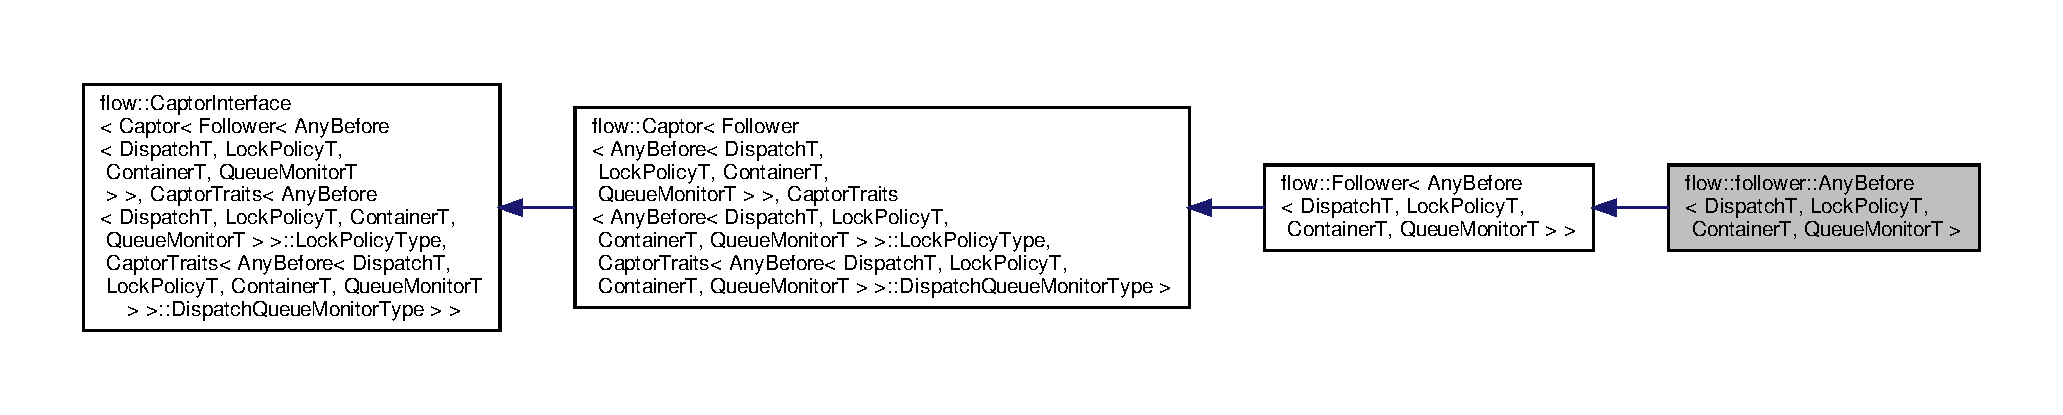
\includegraphics[width=350pt]{classflow_1_1follower_1_1_any_before__inherit__graph}
\end{center}
\end{figure}


Collaboration diagram for flow\+:\+:follower\+:\+:Any\+Before$<$ DispatchT, Lock\+PolicyT, ContainerT, Queue\+MonitorT $>$\+:
\nopagebreak
\begin{figure}[H]
\begin{center}
\leavevmode
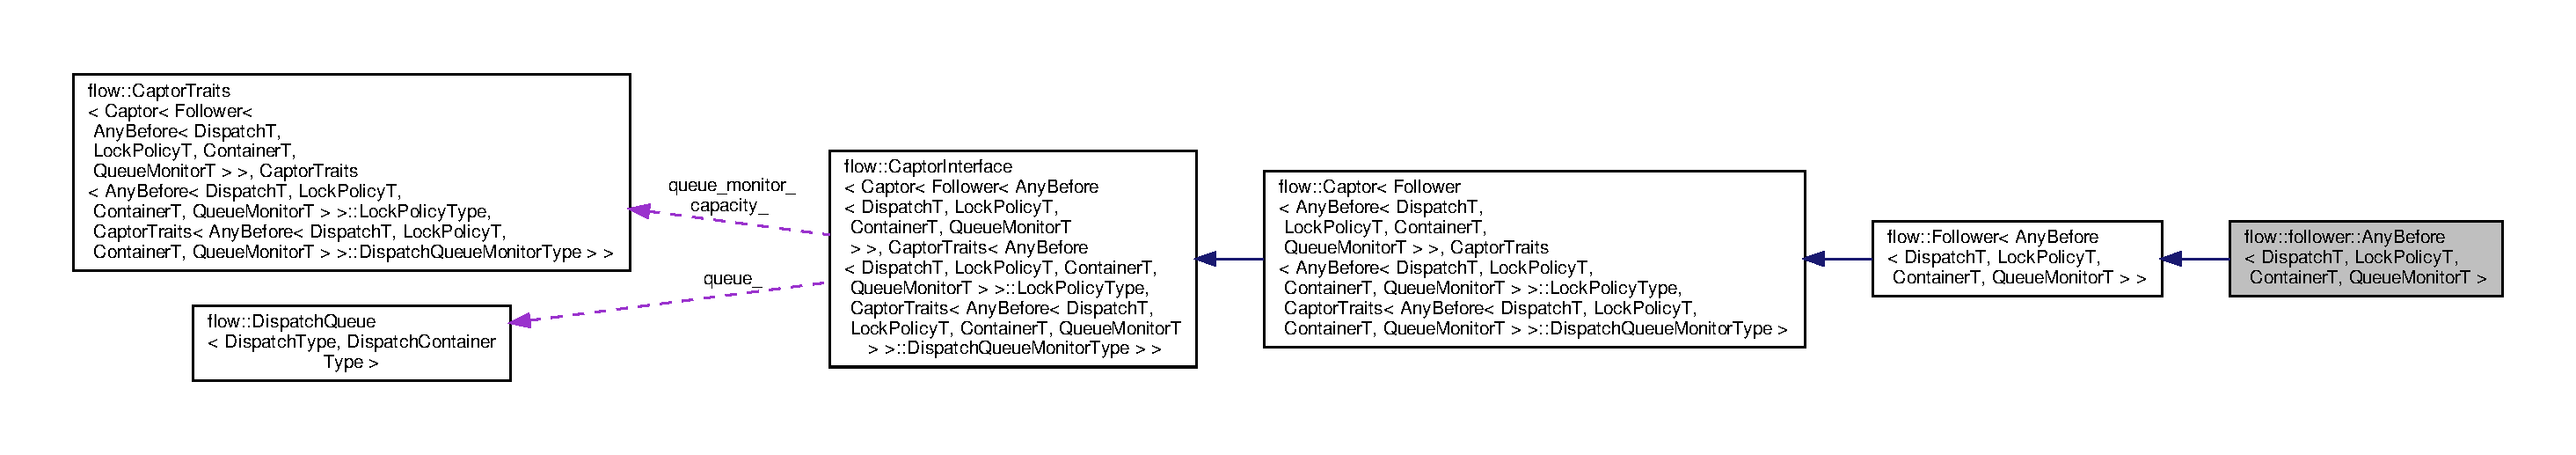
\includegraphics[width=350pt]{classflow_1_1follower_1_1_any_before__coll__graph}
\end{center}
\end{figure}
\subsection*{Public Types}
\begin{DoxyCompactItemize}
\item 
\mbox{\Hypertarget{classflow_1_1follower_1_1_any_before_a314362d61e731cdffefbcbf0e12dd6d8}\label{classflow_1_1follower_1_1_any_before_a314362d61e731cdffefbcbf0e12dd6d8}} 
using \hyperlink{classflow_1_1follower_1_1_any_before_a314362d61e731cdffefbcbf0e12dd6d8}{stamp\+\_\+type} = typename \hyperlink{structflow_1_1_captor_traits}{Captor\+Traits}$<$ \hyperlink{classflow_1_1follower_1_1_any_before}{Any\+Before} $>$\+::\hyperlink{classflow_1_1follower_1_1_any_before_a314362d61e731cdffefbcbf0e12dd6d8}{stamp\+\_\+type}
\begin{DoxyCompactList}\small\item\em Data stamp type. \end{DoxyCompactList}\item 
\mbox{\Hypertarget{classflow_1_1follower_1_1_any_before_aee1b47d081b0b242b5fddabcd2c5310c}\label{classflow_1_1follower_1_1_any_before_aee1b47d081b0b242b5fddabcd2c5310c}} 
using \hyperlink{classflow_1_1follower_1_1_any_before_aee1b47d081b0b242b5fddabcd2c5310c}{offset\+\_\+type} = typename \hyperlink{structflow_1_1_captor_traits}{Captor\+Traits}$<$ \hyperlink{classflow_1_1follower_1_1_any_before}{Any\+Before} $>$\+::\hyperlink{classflow_1_1follower_1_1_any_before_aee1b47d081b0b242b5fddabcd2c5310c}{offset\+\_\+type}
\begin{DoxyCompactList}\small\item\em Data stamp duration type. \end{DoxyCompactList}\end{DoxyCompactItemize}
\subsection*{Public Member Functions}
\begin{DoxyCompactItemize}
\item 
\hyperlink{classflow_1_1follower_1_1_any_before_a68131a41e3c0ce8ae050b39080c57371}{Any\+Before} (const \hyperlink{classflow_1_1follower_1_1_any_before_aee1b47d081b0b242b5fddabcd2c5310c}{offset\+\_\+type} \&delay, const ContainerT \&container=ContainerT\{\}, const Queue\+MonitorT \&queue\+\_\+monitor=Queue\+MonitorT\{\})
\begin{DoxyCompactList}\small\item\em Setup constructor. \end{DoxyCompactList}\end{DoxyCompactItemize}
\subsection*{Additional Inherited Members}


\subsection{Detailed Description}
\subsubsection*{template$<$typename DispatchT, typename Lock\+PolicyT = No\+Lock, typename ContainerT = Default\+Container$<$\+Dispatch\+T$>$, typename Queue\+MonitorT = Default\+Dispatch\+Queue\+Monitor$>$\newline
class flow\+::follower\+::\+Any\+Before$<$ Dispatch\+T, Lock\+Policy\+T, Container\+T, Queue\+Monitor\+T $>$}

Captures all data elements from a delay before the driving sequencing stamp. 

This capture buffer will capture data which is behind the driving upper sequence stamp ({\ttfamily range.\+upper\+\_\+stamp}) by some sequencing delay w.\+r.\+t a driver-\/provided target time. It will return all data at and before that sequencing boundary that has not previously been captured. ~\newline
 This capture buffer is always ready, and will always return with a P\+R\+I\+M\+ED state, regardless of whether or not there is data available to capture. ~\newline
 {\bfseries Data removal\+:} \hyperlink{classflow_1_1_captor}{Captor} will remove all data before the driving time message minus the delay


\begin{DoxyTemplParams}{Template Parameters}
{\em DispatchT} & data dispatch type \\
\hline
{\em Lock\+PolicyT} & a Basic\+Lockable (\href{https://en.cppreference.com/w/cpp/named_req/BasicLockable}{\tt https\+://en.\+cppreference.\+com/w/cpp/named\+\_\+req/\+Basic\+Lockable}) object or \hyperlink{structflow_1_1_no_lock}{No\+Lock} or \hyperlink{structflow_1_1_polling_lock}{Polling\+Lock} \\
\hline
{\em ContainerT} & underlying {\ttfamily DispatchT} container type \\
\hline
{\em Queue\+MonitorT} & object used to monitor queue state on each insertion; used to precondition capture\\
\hline
\end{DoxyTemplParams}
This captor W\+I\+LL N\+OT behave deterministically if all data is not available before capture time minus the specified delay. As such, setting the delay properly will alleviate non-\/deterministic behavior. This is the only {\itshape optional} captor, and should be used with great caution. 

\subsection{Constructor \& Destructor Documentation}
\mbox{\Hypertarget{classflow_1_1follower_1_1_any_before_a68131a41e3c0ce8ae050b39080c57371}\label{classflow_1_1follower_1_1_any_before_a68131a41e3c0ce8ae050b39080c57371}} 
\index{flow\+::follower\+::\+Any\+Before@{flow\+::follower\+::\+Any\+Before}!Any\+Before@{Any\+Before}}
\index{Any\+Before@{Any\+Before}!flow\+::follower\+::\+Any\+Before@{flow\+::follower\+::\+Any\+Before}}
\subsubsection{\texorpdfstring{Any\+Before()}{AnyBefore()}}
{\footnotesize\ttfamily template$<$typename DispatchT , typename Lock\+PolicyT  = No\+Lock, typename ContainerT  = Default\+Container$<$\+Dispatch\+T$>$, typename Queue\+MonitorT  = Default\+Dispatch\+Queue\+Monitor$>$ \\
\hyperlink{classflow_1_1follower_1_1_any_before}{flow\+::follower\+::\+Any\+Before}$<$ DispatchT, Lock\+PolicyT, ContainerT, Queue\+MonitorT $>$\+::\hyperlink{classflow_1_1follower_1_1_any_before}{Any\+Before} (\begin{DoxyParamCaption}\item[{const \hyperlink{classflow_1_1follower_1_1_any_before_aee1b47d081b0b242b5fddabcd2c5310c}{offset\+\_\+type} \&}]{delay,  }\item[{const ContainerT \&}]{container = {\ttfamily ContainerT\{\}},  }\item[{const Queue\+MonitorT \&}]{queue\+\_\+monitor = {\ttfamily QueueMonitorT\{\}} }\end{DoxyParamCaption})\hspace{0.3cm}{\ttfamily [explicit]}}



Setup constructor. 


\begin{DoxyParams}{Parameters}
{\em delay} & the delay with which to capture \\
\hline
{\em container} & container object with some initial state \\
\hline
{\em queue\+\_\+monitor} & queue monitor with some initial state \\
\hline
\end{DoxyParams}


The documentation for this class was generated from the following file\+:\begin{DoxyCompactItemize}
\item 
flow/include/follower/any\+\_\+before.\+h\end{DoxyCompactItemize}

\hypertarget{classflow_1_1driver_1_1_batch}{}\section{flow\+:\+:driver\+:\+:Batch$<$ DispatchT, Lock\+PolicyT, ContainerT, Queue\+MonitorT $>$ Class Template Reference}
\label{classflow_1_1driver_1_1_batch}\index{flow\+::driver\+::\+Batch$<$ Dispatch\+T, Lock\+Policy\+T, Container\+T, Queue\+Monitor\+T $>$@{flow\+::driver\+::\+Batch$<$ Dispatch\+T, Lock\+Policy\+T, Container\+T, Queue\+Monitor\+T $>$}}


Captures the N oldest data elements.  




{\ttfamily \#include $<$batch.\+h$>$}



Inheritance diagram for flow\+:\+:driver\+:\+:Batch$<$ DispatchT, Lock\+PolicyT, ContainerT, Queue\+MonitorT $>$\+:
\nopagebreak
\begin{figure}[H]
\begin{center}
\leavevmode
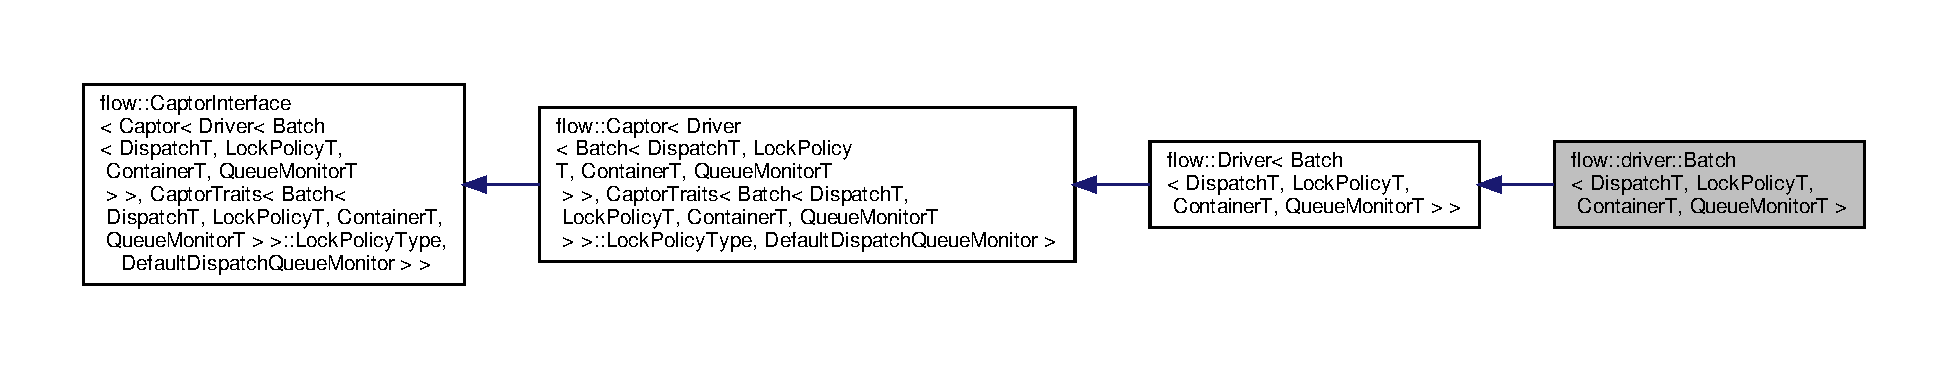
\includegraphics[width=350pt]{classflow_1_1driver_1_1_batch__inherit__graph}
\end{center}
\end{figure}


Collaboration diagram for flow\+:\+:driver\+:\+:Batch$<$ DispatchT, Lock\+PolicyT, ContainerT, Queue\+MonitorT $>$\+:
\nopagebreak
\begin{figure}[H]
\begin{center}
\leavevmode
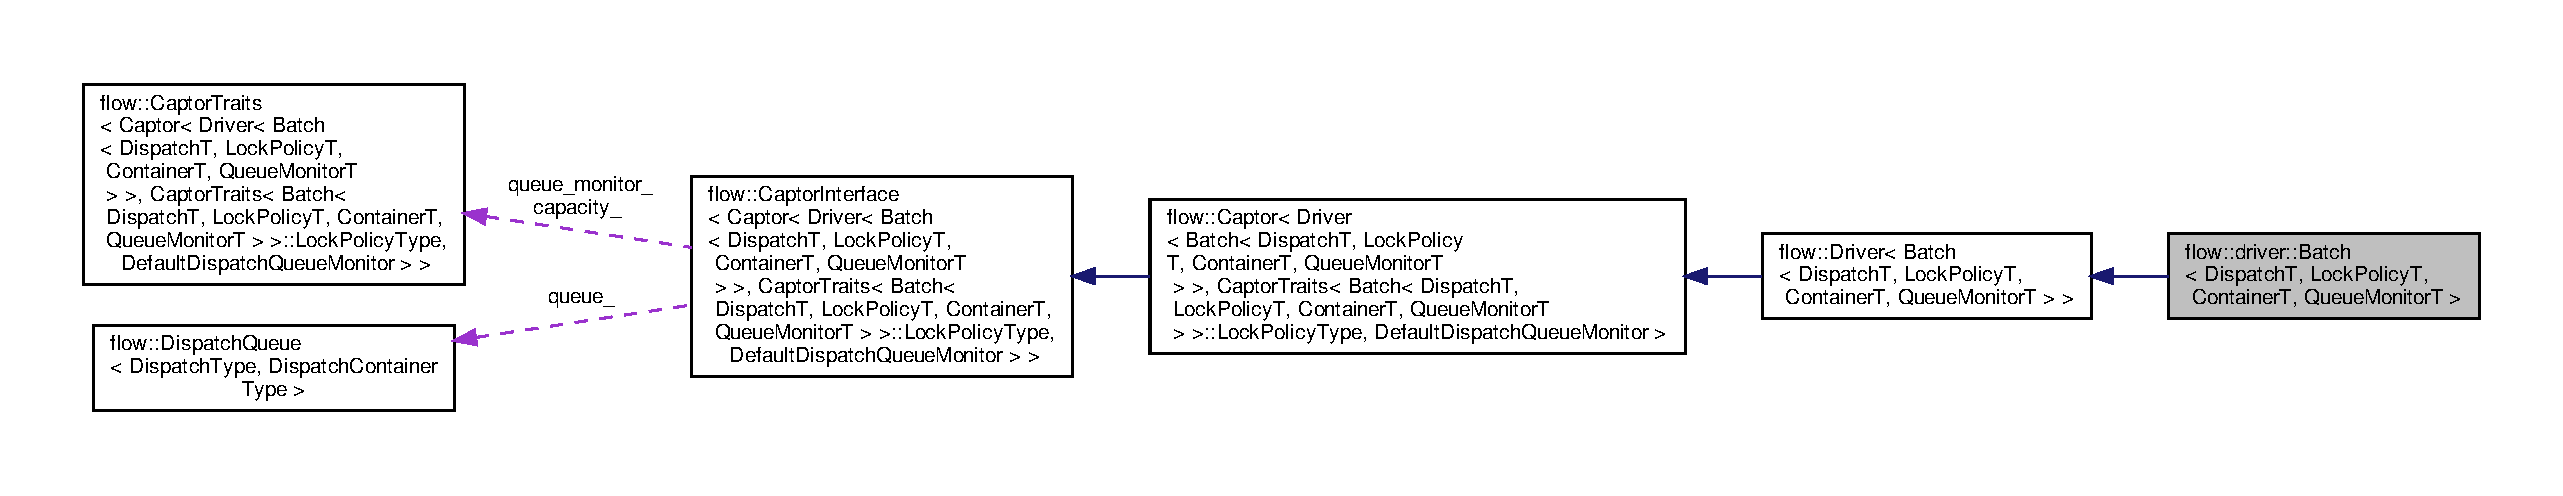
\includegraphics[width=350pt]{classflow_1_1driver_1_1_batch__coll__graph}
\end{center}
\end{figure}
\subsection*{Public Types}
\begin{DoxyCompactItemize}
\item 
\mbox{\Hypertarget{classflow_1_1driver_1_1_batch_a81f688882ffe1a15ab3d8af872ffe6f7}\label{classflow_1_1driver_1_1_batch_a81f688882ffe1a15ab3d8af872ffe6f7}} 
using \hyperlink{classflow_1_1driver_1_1_batch_a81f688882ffe1a15ab3d8af872ffe6f7}{size\+\_\+type} = typename \hyperlink{structflow_1_1_captor_traits}{Captor\+Traits}$<$ \hyperlink{classflow_1_1driver_1_1_batch}{Batch} $>$\+::\hyperlink{classflow_1_1driver_1_1_batch_a81f688882ffe1a15ab3d8af872ffe6f7}{size\+\_\+type}
\begin{DoxyCompactList}\small\item\em Integer size type. \end{DoxyCompactList}\item 
\mbox{\Hypertarget{classflow_1_1driver_1_1_batch_af28211948e71149b26cff0e2345b830f}\label{classflow_1_1driver_1_1_batch_af28211948e71149b26cff0e2345b830f}} 
using \hyperlink{classflow_1_1driver_1_1_batch_af28211948e71149b26cff0e2345b830f}{stamp\+\_\+type} = typename \hyperlink{structflow_1_1_captor_traits}{Captor\+Traits}$<$ \hyperlink{classflow_1_1driver_1_1_batch}{Batch} $>$\+::\hyperlink{classflow_1_1driver_1_1_batch_af28211948e71149b26cff0e2345b830f}{stamp\+\_\+type}
\begin{DoxyCompactList}\small\item\em Data stamp type. \end{DoxyCompactList}\end{DoxyCompactItemize}
\subsection*{Public Member Functions}
\begin{DoxyCompactItemize}
\item 
\hyperlink{classflow_1_1driver_1_1_batch_a021d7a60b375a2fea3716deb6e709487}{Batch} (const \hyperlink{classflow_1_1driver_1_1_batch_a81f688882ffe1a15ab3d8af872ffe6f7}{size\+\_\+type} \hyperlink{classflow_1_1_captor_interface_a1a4b3f7f6c1bd16a2cb672d90a1cbbc0}{size}, const ContainerT \&container=ContainerT\{\}, const Queue\+MonitorT \&queue\+\_\+monitor=Queue\+MonitorT\{\}) noexcept(false)
\begin{DoxyCompactList}\small\item\em Configuration constructor. \end{DoxyCompactList}\end{DoxyCompactItemize}
\subsection*{Additional Inherited Members}


\subsection{Detailed Description}
\subsubsection*{template$<$typename DispatchT, typename Lock\+PolicyT = No\+Lock, typename ContainerT = Default\+Container$<$\+Dispatch\+T$>$, typename Queue\+MonitorT = Default\+Dispatch\+Queue\+Monitor$>$\newline
class flow\+::driver\+::\+Batch$<$ Dispatch\+T, Lock\+Policy\+T, Container\+T, Queue\+Monitor\+T $>$}

Captures the N oldest data elements. 

Establishes a sequencing range with where {\ttfamily range.\+lower\+\_\+stamp} is the stamp of the oldest captured element, and {\ttfamily range.\+upper\+\_\+stamp} is the stamp of the newest. Removes oldest captured element from buffer.


\begin{DoxyTemplParams}{Template Parameters}
{\em DispatchT} & data dispatch type \\
\hline
{\em Lock\+PolicyT} & a Basic\+Lockable (\href{https://en.cppreference.com/w/cpp/named_req/BasicLockable}{\tt https\+://en.\+cppreference.\+com/w/cpp/named\+\_\+req/\+Basic\+Lockable}) object or \hyperlink{structflow_1_1_no_lock}{No\+Lock} or \hyperlink{structflow_1_1_polling_lock}{Polling\+Lock} \\
\hline
{\em ContainerT} & underlying {\ttfamily DispatchT} container type \\
\hline
{\em Queue\+MonitorT} & object used to monitor queue state on each insertion \\
\hline
\end{DoxyTemplParams}


\subsection{Constructor \& Destructor Documentation}
\mbox{\Hypertarget{classflow_1_1driver_1_1_batch_a021d7a60b375a2fea3716deb6e709487}\label{classflow_1_1driver_1_1_batch_a021d7a60b375a2fea3716deb6e709487}} 
\index{flow\+::driver\+::\+Batch@{flow\+::driver\+::\+Batch}!Batch@{Batch}}
\index{Batch@{Batch}!flow\+::driver\+::\+Batch@{flow\+::driver\+::\+Batch}}
\subsubsection{\texorpdfstring{Batch()}{Batch()}}
{\footnotesize\ttfamily template$<$typename DispatchT , typename Lock\+PolicyT  = No\+Lock, typename ContainerT  = Default\+Container$<$\+Dispatch\+T$>$, typename Queue\+MonitorT  = Default\+Dispatch\+Queue\+Monitor$>$ \\
\hyperlink{classflow_1_1driver_1_1_batch}{flow\+::driver\+::\+Batch}$<$ DispatchT, Lock\+PolicyT, ContainerT, Queue\+MonitorT $>$\+::\hyperlink{classflow_1_1driver_1_1_batch}{Batch} (\begin{DoxyParamCaption}\item[{const \hyperlink{classflow_1_1driver_1_1_batch_a81f688882ffe1a15ab3d8af872ffe6f7}{size\+\_\+type}}]{size,  }\item[{const ContainerT \&}]{container = {\ttfamily ContainerT\{\}},  }\item[{const Queue\+MonitorT \&}]{queue\+\_\+monitor = {\ttfamily QueueMonitorT\{\}} }\end{DoxyParamCaption})\hspace{0.3cm}{\ttfamily [explicit]}, {\ttfamily [noexcept]}}



Configuration constructor. 


\begin{DoxyParams}{Parameters}
{\em size} & number of elements to batch before becoming ready \\
\hline
{\em container} & container object with some initial state\\
\hline
\end{DoxyParams}

\begin{DoxyExceptions}{Exceptions}
{\em $<$code$>$std\+::invalid\+\_\+argument$<$/code$>$} & if {\ttfamily size == 0} \\
\hline
{\em $<$code$>$std\+::invalid\+\_\+argument$<$/code$>$} & if {\ttfamily Capture\+OutputT} cannot hold {\ttfamily size} \\
\hline
\end{DoxyExceptions}


The documentation for this class was generated from the following file\+:\begin{DoxyCompactItemize}
\item 
flow/include/driver/\hyperlink{batch_8h}{batch.\+h}\end{DoxyCompactItemize}

\hypertarget{classflow_1_1follower_1_1_before}{}\section{flow\+:\+:follower\+:\+:Before$<$ DispatchT, Lock\+PolicyT, ContainerT, Queue\+MonitorT $>$ Class Template Reference}
\label{classflow_1_1follower_1_1_before}\index{flow\+::follower\+::\+Before$<$ Dispatch\+T, Lock\+Policy\+T, Container\+T, Queue\+Monitor\+T $>$@{flow\+::follower\+::\+Before$<$ Dispatch\+T, Lock\+Policy\+T, Container\+T, Queue\+Monitor\+T $>$}}


Captures all elements before the capture range lower bound, minus a delay period.  




{\ttfamily \#include $<$before.\+h$>$}



Inheritance diagram for flow\+:\+:follower\+:\+:Before$<$ DispatchT, Lock\+PolicyT, ContainerT, Queue\+MonitorT $>$\+:
\nopagebreak
\begin{figure}[H]
\begin{center}
\leavevmode
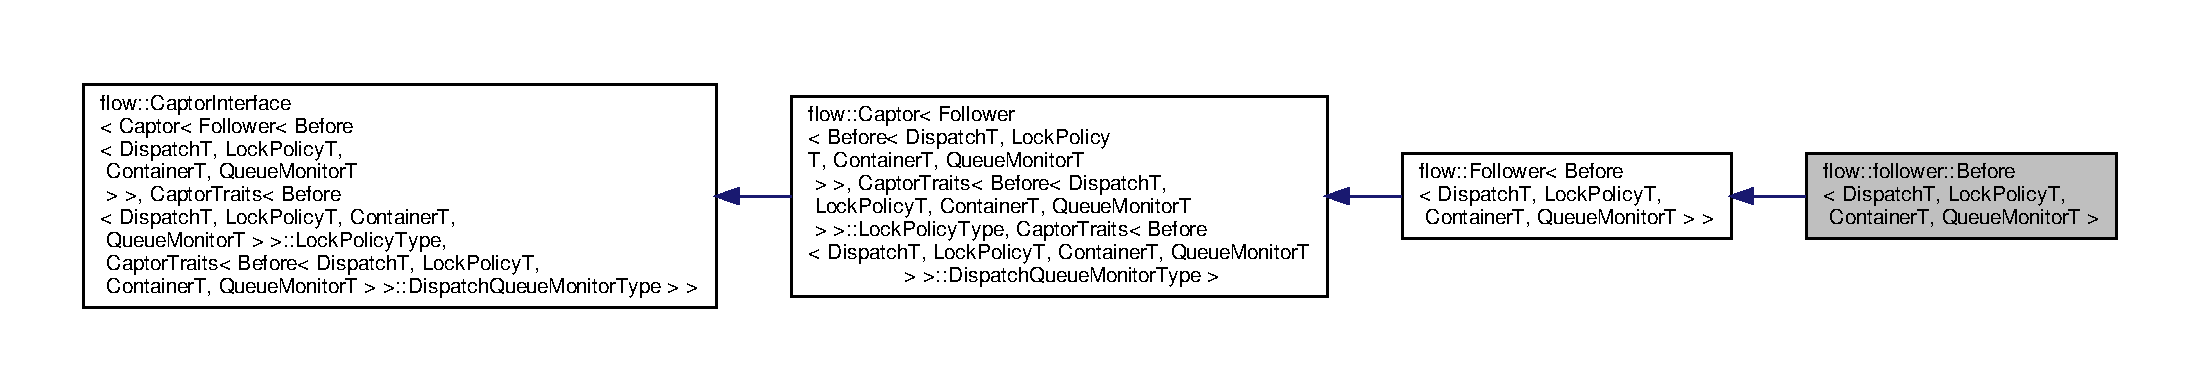
\includegraphics[width=350pt]{classflow_1_1follower_1_1_before__inherit__graph}
\end{center}
\end{figure}


Collaboration diagram for flow\+:\+:follower\+:\+:Before$<$ DispatchT, Lock\+PolicyT, ContainerT, Queue\+MonitorT $>$\+:
\nopagebreak
\begin{figure}[H]
\begin{center}
\leavevmode
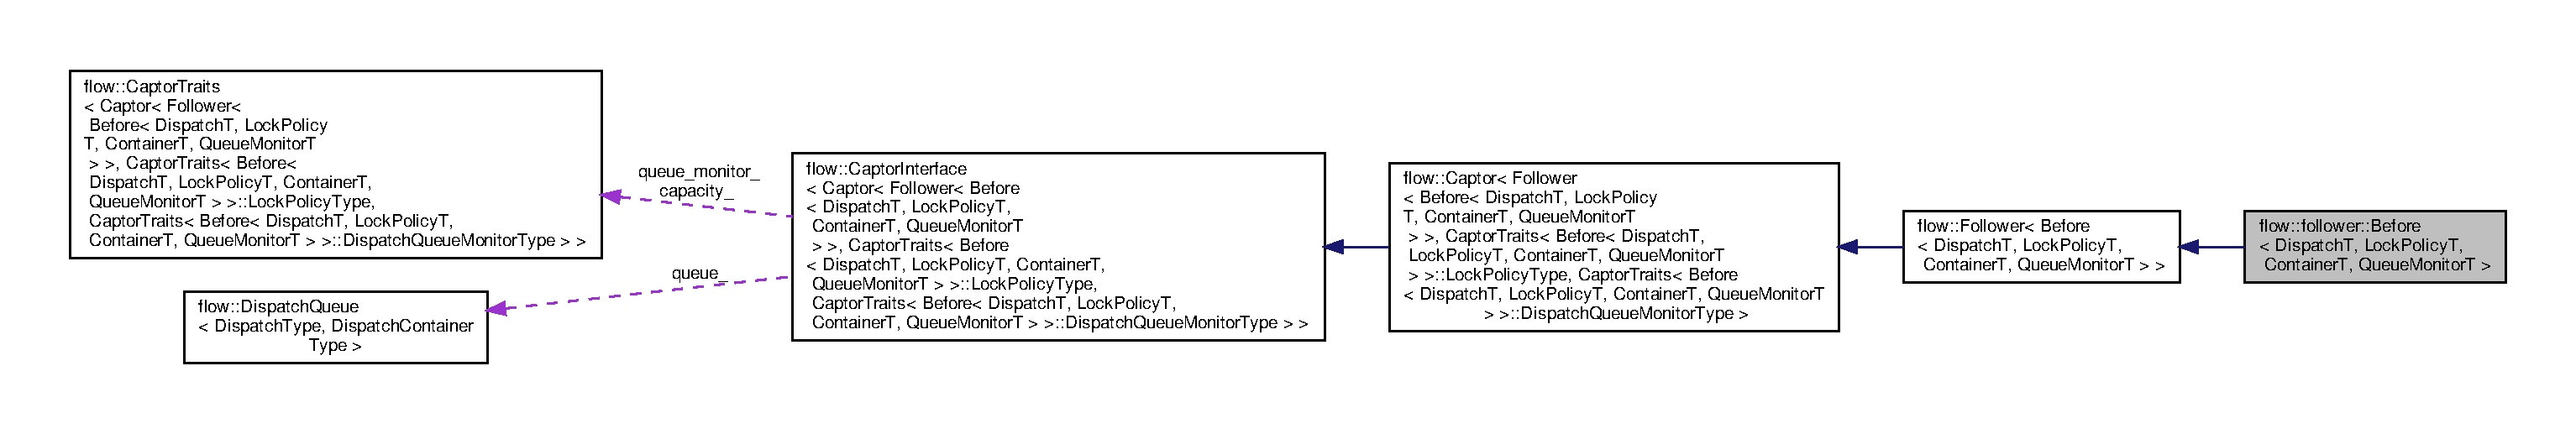
\includegraphics[width=350pt]{classflow_1_1follower_1_1_before__coll__graph}
\end{center}
\end{figure}
\subsection*{Public Types}
\begin{DoxyCompactItemize}
\item 
\mbox{\Hypertarget{classflow_1_1follower_1_1_before_afd0adcf4c1d76dce28f8856f25347aa7}\label{classflow_1_1follower_1_1_before_afd0adcf4c1d76dce28f8856f25347aa7}} 
using \hyperlink{classflow_1_1follower_1_1_before_afd0adcf4c1d76dce28f8856f25347aa7}{stamp\+\_\+type} = typename \hyperlink{structflow_1_1_captor_traits}{Captor\+Traits}$<$ \hyperlink{classflow_1_1follower_1_1_before}{Before} $>$\+::\hyperlink{classflow_1_1follower_1_1_before_afd0adcf4c1d76dce28f8856f25347aa7}{stamp\+\_\+type}
\begin{DoxyCompactList}\small\item\em Data stamp type. \end{DoxyCompactList}\item 
\mbox{\Hypertarget{classflow_1_1follower_1_1_before_a5bb9194263576cac18c7e602ab33e7b4}\label{classflow_1_1follower_1_1_before_a5bb9194263576cac18c7e602ab33e7b4}} 
using \hyperlink{classflow_1_1follower_1_1_before_a5bb9194263576cac18c7e602ab33e7b4}{offset\+\_\+type} = typename \hyperlink{structflow_1_1_captor_traits}{Captor\+Traits}$<$ \hyperlink{classflow_1_1follower_1_1_before}{Before} $>$\+::\hyperlink{classflow_1_1follower_1_1_before_a5bb9194263576cac18c7e602ab33e7b4}{offset\+\_\+type}
\begin{DoxyCompactList}\small\item\em Data stamp duration type. \end{DoxyCompactList}\end{DoxyCompactItemize}
\subsection*{Public Member Functions}
\begin{DoxyCompactItemize}
\item 
\hyperlink{classflow_1_1follower_1_1_before_a8245d0990db036bd525f3534ef7876bb}{Before} (const \hyperlink{classflow_1_1follower_1_1_before_a5bb9194263576cac18c7e602ab33e7b4}{offset\+\_\+type} \&delay, const ContainerT \&container=ContainerT\{\}, const Queue\+MonitorT \&queue\+\_\+monitor=Queue\+MonitorT\{\})
\begin{DoxyCompactList}\small\item\em Setup constructor. \end{DoxyCompactList}\end{DoxyCompactItemize}
\subsection*{Additional Inherited Members}


\subsection{Detailed Description}
\subsubsection*{template$<$typename DispatchT, typename Lock\+PolicyT = No\+Lock, typename ContainerT = Default\+Container$<$\+Dispatch\+T$>$, typename Queue\+MonitorT = Default\+Dispatch\+Queue\+Monitor$>$\newline
class flow\+::follower\+::\+Before$<$ Dispatch\+T, Lock\+Policy\+T, Container\+T, Queue\+Monitor\+T $>$}

Captures all elements before the capture range lower bound, minus a delay period. 

Once at least a single element is available after said sequencing boundary. All of the captured elements are removed.


\begin{DoxyTemplParams}{Template Parameters}
{\em DispatchT} & data dispatch type \\
\hline
{\em Lock\+PolicyT} & a Basic\+Lockable (\href{https://en.cppreference.com/w/cpp/named_req/BasicLockable}{\tt https\+://en.\+cppreference.\+com/w/cpp/named\+\_\+req/\+Basic\+Lockable}) object or \hyperlink{structflow_1_1_no_lock}{No\+Lock} or \hyperlink{structflow_1_1_polling_lock}{Polling\+Lock} \\
\hline
{\em ContainerT} & underlying {\ttfamily DispatchT} container type \\
\hline
{\em Queue\+MonitorT} & object used to monitor queue state on each insertion; used to precondition capture \\
\hline
\end{DoxyTemplParams}


\subsection{Constructor \& Destructor Documentation}
\mbox{\Hypertarget{classflow_1_1follower_1_1_before_a8245d0990db036bd525f3534ef7876bb}\label{classflow_1_1follower_1_1_before_a8245d0990db036bd525f3534ef7876bb}} 
\index{flow\+::follower\+::\+Before@{flow\+::follower\+::\+Before}!Before@{Before}}
\index{Before@{Before}!flow\+::follower\+::\+Before@{flow\+::follower\+::\+Before}}
\subsubsection{\texorpdfstring{Before()}{Before()}}
{\footnotesize\ttfamily template$<$typename DispatchT , typename Lock\+PolicyT  = No\+Lock, typename ContainerT  = Default\+Container$<$\+Dispatch\+T$>$, typename Queue\+MonitorT  = Default\+Dispatch\+Queue\+Monitor$>$ \\
\hyperlink{classflow_1_1follower_1_1_before}{flow\+::follower\+::\+Before}$<$ DispatchT, Lock\+PolicyT, ContainerT, Queue\+MonitorT $>$\+::\hyperlink{classflow_1_1follower_1_1_before}{Before} (\begin{DoxyParamCaption}\item[{const \hyperlink{classflow_1_1follower_1_1_before_a5bb9194263576cac18c7e602ab33e7b4}{offset\+\_\+type} \&}]{delay,  }\item[{const ContainerT \&}]{container = {\ttfamily ContainerT\{\}},  }\item[{const Queue\+MonitorT \&}]{queue\+\_\+monitor = {\ttfamily QueueMonitorT\{\}} }\end{DoxyParamCaption})\hspace{0.3cm}{\ttfamily [explicit]}}



Setup constructor. 


\begin{DoxyParams}{Parameters}
{\em delay} & the delay with which to capture \\
\hline
{\em container} & container object with some initial state \\
\hline
{\em queue\+\_\+monitor} & queue monitor with some initial state \\
\hline
\end{DoxyParams}


The documentation for this class was generated from the following file\+:\begin{DoxyCompactItemize}
\item 
flow/include/follower/\hyperlink{before_8h}{before.\+h}\end{DoxyCompactItemize}

\hypertarget{classflow_1_1_captor}{}\section{flow\+:\+:Captor$<$ CaptorT, LockableT, Queue\+MonitorT $>$ Class Template Reference}
\label{classflow_1_1_captor}\index{flow\+::\+Captor$<$ Captor\+T, Lockable\+T, Queue\+Monitor\+T $>$@{flow\+::\+Captor$<$ Captor\+T, Lockable\+T, Queue\+Monitor\+T $>$}}


C\+R\+T\+P-\/base for input capture buffers with a specific data lock policy.  




{\ttfamily \#include $<$captor.\+h$>$}



Inheritance diagram for flow\+:\+:Captor$<$ CaptorT, LockableT, Queue\+MonitorT $>$\+:
\nopagebreak
\begin{figure}[H]
\begin{center}
\leavevmode
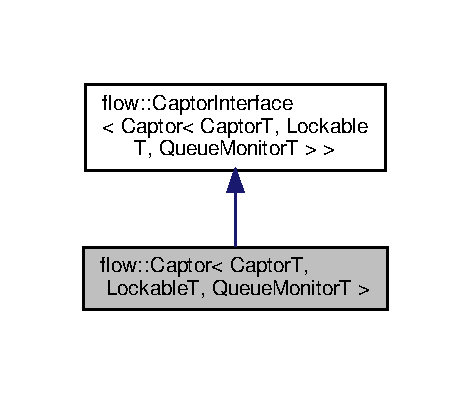
\includegraphics[width=226pt]{classflow_1_1_captor__inherit__graph}
\end{center}
\end{figure}


Collaboration diagram for flow\+:\+:Captor$<$ CaptorT, LockableT, Queue\+MonitorT $>$\+:
\nopagebreak
\begin{figure}[H]
\begin{center}
\leavevmode
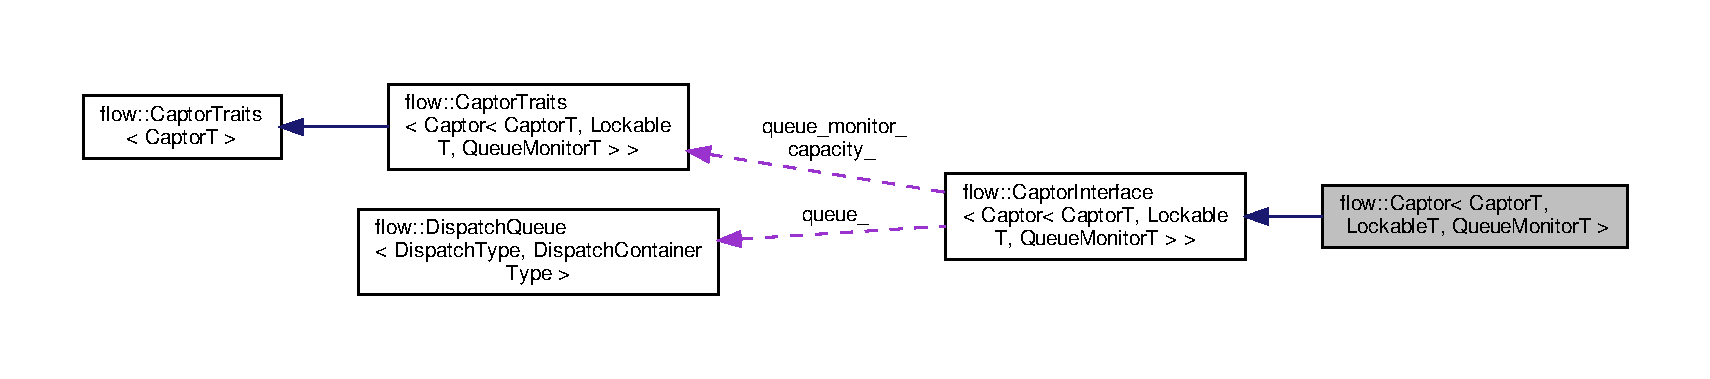
\includegraphics[width=350pt]{classflow_1_1_captor__coll__graph}
\end{center}
\end{figure}
\subsection*{Public Types}
\begin{DoxyCompactItemize}
\item 
\mbox{\Hypertarget{classflow_1_1_captor_a6dd5c26329b3c721362f58c5a0a2bc1b}\label{classflow_1_1_captor_a6dd5c26329b3c721362f58c5a0a2bc1b}} 
using \hyperlink{classflow_1_1_captor_a6dd5c26329b3c721362f58c5a0a2bc1b}{Dispatch\+Type} = typename \hyperlink{structflow_1_1_captor_traits}{Captor\+Traits}$<$ CaptorT $>$\+::\hyperlink{classflow_1_1_captor_a6dd5c26329b3c721362f58c5a0a2bc1b}{Dispatch\+Type}
\begin{DoxyCompactList}\small\item\em Data dispatch type. \end{DoxyCompactList}\item 
\mbox{\Hypertarget{classflow_1_1_captor_a9dce19a6644e31358099f2aeb1873b6a}\label{classflow_1_1_captor_a9dce19a6644e31358099f2aeb1873b6a}} 
using \hyperlink{classflow_1_1_captor_a9dce19a6644e31358099f2aeb1873b6a}{Dispatch\+Container\+Type} = typename \hyperlink{structflow_1_1_captor_traits}{Captor\+Traits}$<$ CaptorT $>$\+::\hyperlink{classflow_1_1_captor_a9dce19a6644e31358099f2aeb1873b6a}{Dispatch\+Container\+Type}
\begin{DoxyCompactList}\small\item\em Data dispatch container type. \end{DoxyCompactList}\item 
\mbox{\Hypertarget{classflow_1_1_captor_a266a9d119a209ebe389dde77c5aa7af6}\label{classflow_1_1_captor_a266a9d119a209ebe389dde77c5aa7af6}} 
using \hyperlink{classflow_1_1_captor_a266a9d119a209ebe389dde77c5aa7af6}{stamp\+\_\+type} = typename \hyperlink{structflow_1_1_captor_traits}{Captor\+Traits}$<$ CaptorT $>$\+::\hyperlink{classflow_1_1_captor_a266a9d119a209ebe389dde77c5aa7af6}{stamp\+\_\+type}
\begin{DoxyCompactList}\small\item\em Data stamp type. \end{DoxyCompactList}\item 
\mbox{\Hypertarget{classflow_1_1_captor_a8a0e689ccd2e1874f3c2f13cf18eb386}\label{classflow_1_1_captor_a8a0e689ccd2e1874f3c2f13cf18eb386}} 
using \hyperlink{classflow_1_1_captor_a8a0e689ccd2e1874f3c2f13cf18eb386}{size\+\_\+type} = typename \hyperlink{structflow_1_1_captor_traits}{Captor\+Traits}$<$ CaptorT $>$\+::\hyperlink{classflow_1_1_captor_a8a0e689ccd2e1874f3c2f13cf18eb386}{size\+\_\+type}
\begin{DoxyCompactList}\small\item\em Integer size type. \end{DoxyCompactList}\end{DoxyCompactItemize}
\subsection*{Public Member Functions}
\begin{DoxyCompactItemize}
\item 
\mbox{\Hypertarget{classflow_1_1_captor_a88157a75b4bd2db2673bc5c0287669fe}\label{classflow_1_1_captor_a88157a75b4bd2db2673bc5c0287669fe}} 
\hyperlink{classflow_1_1_captor_a88157a75b4bd2db2673bc5c0287669fe}{Captor} ()
\begin{DoxyCompactList}\small\item\em Default constructor. \end{DoxyCompactList}\item 
\hyperlink{classflow_1_1_captor_ab5d0d53e66fae964b39c80eb28092a29}{Captor} (const \hyperlink{classflow_1_1_captor_a9dce19a6644e31358099f2aeb1873b6a}{Dispatch\+Container\+Type} \&container, const Queue\+MonitorT \&queue\+\_\+monitor)
\begin{DoxyCompactList}\small\item\em \hyperlink{classflow_1_1_dispatch}{Dispatch} container constructor. \end{DoxyCompactList}\item 
\hyperlink{classflow_1_1_captor_a6d3e5ade0abc054ef81dedfa05a8b55b}{$\sim$\+Captor} ()
\begin{DoxyCompactList}\small\item\em Destructor. \end{DoxyCompactList}\end{DoxyCompactItemize}
\subsection*{Additional Inherited Members}


\subsection{Detailed Description}
\subsubsection*{template$<$typename CaptorT, typename LockableT, typename Queue\+MonitorT$>$\newline
class flow\+::\+Captor$<$ Captor\+T, Lockable\+T, Queue\+Monitor\+T $>$}

C\+R\+T\+P-\/base for input capture buffers with a specific data lock policy. 


\begin{DoxyTemplParams}{Template Parameters}
{\em CaptorT} & C\+R\+T\+P-\/derived \hyperlink{classflow_1_1_captor}{Captor} type \\
\hline
{\em LockableT} & a Timed\+Lockable (\href{https://en.cppreference.com/w/cpp/named_req/TimedLockable}{\tt https\+://en.\+cppreference.\+com/w/cpp/named\+\_\+req/\+Timed\+Lockable}) object; specializations are available which replace {\ttfamily LockableT} with {\ttfamily \hyperlink{structflow_1_1_no_lock}{No\+Lock}} or {\ttfamily \hyperlink{structflow_1_1_polling_lock}{Polling\+Lock}} \\
\hline
{\em Queue\+MonitorT} & object used to monitor queue state on each insertion; used to precondition capture \\
\hline
\end{DoxyTemplParams}


\subsection{Constructor \& Destructor Documentation}
\mbox{\Hypertarget{classflow_1_1_captor_ab5d0d53e66fae964b39c80eb28092a29}\label{classflow_1_1_captor_ab5d0d53e66fae964b39c80eb28092a29}} 
\index{flow\+::\+Captor@{flow\+::\+Captor}!Captor@{Captor}}
\index{Captor@{Captor}!flow\+::\+Captor@{flow\+::\+Captor}}
\subsubsection{\texorpdfstring{Captor()}{Captor()}}
{\footnotesize\ttfamily template$<$typename CaptorT, typename LockableT, typename Queue\+MonitorT$>$ \\
\hyperlink{classflow_1_1_captor}{flow\+::\+Captor}$<$ CaptorT, LockableT, Queue\+MonitorT $>$\+::\hyperlink{classflow_1_1_captor}{Captor} (\begin{DoxyParamCaption}\item[{const \hyperlink{classflow_1_1_captor_a9dce19a6644e31358099f2aeb1873b6a}{Dispatch\+Container\+Type} \&}]{container,  }\item[{const Queue\+MonitorT \&}]{queue\+\_\+monitor }\end{DoxyParamCaption})}



\hyperlink{classflow_1_1_dispatch}{Dispatch} container constructor. 


\begin{DoxyParams}{Parameters}
{\em container} & container object with some initial state \\
\hline
{\em queue\+\_\+monitor} & queue monitor with some initial state \\
\hline
\end{DoxyParams}
\mbox{\Hypertarget{classflow_1_1_captor_a6d3e5ade0abc054ef81dedfa05a8b55b}\label{classflow_1_1_captor_a6d3e5ade0abc054ef81dedfa05a8b55b}} 
\index{flow\+::\+Captor@{flow\+::\+Captor}!````~Captor@{$\sim$\+Captor}}
\index{````~Captor@{$\sim$\+Captor}!flow\+::\+Captor@{flow\+::\+Captor}}
\subsubsection{\texorpdfstring{$\sim$\+Captor()}{~Captor()}}
{\footnotesize\ttfamily template$<$typename CaptorT, typename LockableT, typename Queue\+MonitorT$>$ \\
\hyperlink{classflow_1_1_captor}{flow\+::\+Captor}$<$ CaptorT, LockableT, Queue\+MonitorT $>$\+::$\sim$\hyperlink{classflow_1_1_captor}{Captor} (\begin{DoxyParamCaption}{ }\end{DoxyParamCaption})}



Destructor. 

\begin{DoxyNote}{Note}
Releases data waits 
\end{DoxyNote}


The documentation for this class was generated from the following file\+:\begin{DoxyCompactItemize}
\item 
flow/include/\hyperlink{captor_8h}{captor.\+h}\end{DoxyCompactItemize}

\hypertarget{classflow_1_1_captor_interface}{}\section{flow\+:\+:Captor\+Interface$<$ CaptorT $>$ Class Template Reference}
\label{classflow_1_1_captor_interface}\index{flow\+::\+Captor\+Interface$<$ Captor\+T $>$@{flow\+::\+Captor\+Interface$<$ Captor\+T $>$}}


C\+R\+T\+P-\/base which defines basic captor interface.  




{\ttfamily \#include $<$captor.\+h$>$}



Collaboration diagram for flow\+:\+:Captor\+Interface$<$ CaptorT $>$\+:\nopagebreak
\begin{figure}[H]
\begin{center}
\leavevmode
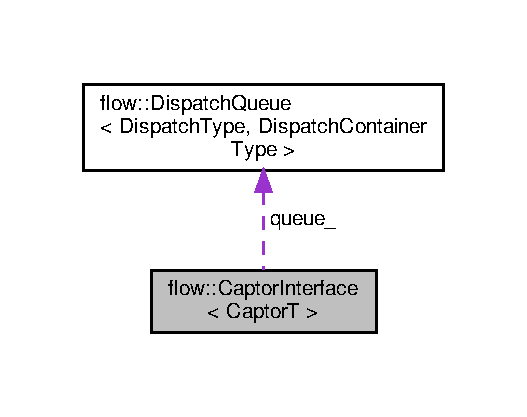
\includegraphics[width=253pt]{classflow_1_1_captor_interface__coll__graph}
\end{center}
\end{figure}
\subsection*{Public Types}
\begin{DoxyCompactItemize}
\item 
\mbox{\Hypertarget{classflow_1_1_captor_interface_ae1eafeb6cd50f4a50843b963c232720a}\label{classflow_1_1_captor_interface_ae1eafeb6cd50f4a50843b963c232720a}} 
using \hyperlink{classflow_1_1_captor_interface_ae1eafeb6cd50f4a50843b963c232720a}{Dispatch\+Type} = typename \hyperlink{structflow_1_1_captor_traits}{Captor\+Traits}$<$ CaptorT $>$\+::\hyperlink{classflow_1_1_captor_interface_ae1eafeb6cd50f4a50843b963c232720a}{Dispatch\+Type}
\begin{DoxyCompactList}\small\item\em Data dispatch type. \end{DoxyCompactList}\item 
\mbox{\Hypertarget{classflow_1_1_captor_interface_a887171bf3b12d8232922a81844ea9a7d}\label{classflow_1_1_captor_interface_a887171bf3b12d8232922a81844ea9a7d}} 
using \hyperlink{classflow_1_1_captor_interface_a887171bf3b12d8232922a81844ea9a7d}{Dispatch\+Container\+Type} = typename \hyperlink{structflow_1_1_captor_traits}{Captor\+Traits}$<$ CaptorT $>$\+::\hyperlink{classflow_1_1_captor_interface_a887171bf3b12d8232922a81844ea9a7d}{Dispatch\+Container\+Type}
\begin{DoxyCompactList}\small\item\em Data dispatch container type. \end{DoxyCompactList}\item 
\mbox{\Hypertarget{classflow_1_1_captor_interface_a6624ec49c575e3a4c2730be405afe179}\label{classflow_1_1_captor_interface_a6624ec49c575e3a4c2730be405afe179}} 
using \hyperlink{classflow_1_1_captor_interface_a6624ec49c575e3a4c2730be405afe179}{Dispatch\+Queue\+Monitor\+Type} = typename \hyperlink{structflow_1_1_captor_traits}{Captor\+Traits}$<$ CaptorT $>$\+::\hyperlink{classflow_1_1_captor_interface_a6624ec49c575e3a4c2730be405afe179}{Dispatch\+Queue\+Monitor\+Type}
\begin{DoxyCompactList}\small\item\em Queue monitor/capture preconditioning type. \end{DoxyCompactList}\item 
\mbox{\Hypertarget{classflow_1_1_captor_interface_a2b87d20d17e8d1437941bd98fe514bc8}\label{classflow_1_1_captor_interface_a2b87d20d17e8d1437941bd98fe514bc8}} 
using \hyperlink{classflow_1_1_captor_interface_a2b87d20d17e8d1437941bd98fe514bc8}{stamp\+\_\+type} = typename \hyperlink{structflow_1_1_captor_traits}{Captor\+Traits}$<$ CaptorT $>$\+::\hyperlink{classflow_1_1_captor_interface_a2b87d20d17e8d1437941bd98fe514bc8}{stamp\+\_\+type}
\begin{DoxyCompactList}\small\item\em Data stamp type. \end{DoxyCompactList}\item 
\mbox{\Hypertarget{classflow_1_1_captor_interface_a62db6a158eebcb377e63ede6a1f1a8c6}\label{classflow_1_1_captor_interface_a62db6a158eebcb377e63ede6a1f1a8c6}} 
using \hyperlink{classflow_1_1_captor_interface_a62db6a158eebcb377e63ede6a1f1a8c6}{size\+\_\+type} = typename \hyperlink{structflow_1_1_captor_traits}{Captor\+Traits}$<$ CaptorT $>$\+::\hyperlink{classflow_1_1_captor_interface_a62db6a158eebcb377e63ede6a1f1a8c6}{size\+\_\+type}
\begin{DoxyCompactList}\small\item\em Integer size type. \end{DoxyCompactList}\end{DoxyCompactItemize}
\subsection*{Public Member Functions}
\begin{DoxyCompactItemize}
\item 
\hyperlink{classflow_1_1_captor_interface_adf956268fd1859bf44c886dc76dadb0b}{Captor\+Interface} (const \hyperlink{classflow_1_1_captor_interface_a62db6a158eebcb377e63ede6a1f1a8c6}{size\+\_\+type} capacity, const \hyperlink{classflow_1_1_captor_interface_a887171bf3b12d8232922a81844ea9a7d}{Dispatch\+Container\+Type} \&container, const \hyperlink{classflow_1_1_captor_interface_a6624ec49c575e3a4c2730be405afe179}{Dispatch\+Queue\+Monitor\+Type} \&queue\+\_\+monitor)
\begin{DoxyCompactList}\small\item\em Full setup constructor. \end{DoxyCompactList}\item 
\mbox{\Hypertarget{classflow_1_1_captor_interface_a78be2f5226c40ef04347d095548b8607}\label{classflow_1_1_captor_interface_a78be2f5226c40ef04347d095548b8607}} 
void \hyperlink{classflow_1_1_captor_interface_a78be2f5226c40ef04347d095548b8607}{reset} ()
\begin{DoxyCompactList}\small\item\em Clears all captor data and resets all states. \end{DoxyCompactList}\item 
\mbox{\Hypertarget{classflow_1_1_captor_interface_a1a4b3f7f6c1bd16a2cb672d90a1cbbc0}\label{classflow_1_1_captor_interface_a1a4b3f7f6c1bd16a2cb672d90a1cbbc0}} 
\hyperlink{classflow_1_1_captor_interface_a62db6a158eebcb377e63ede6a1f1a8c6}{size\+\_\+type} \hyperlink{classflow_1_1_captor_interface_a1a4b3f7f6c1bd16a2cb672d90a1cbbc0}{size} () const
\begin{DoxyCompactList}\small\item\em Returns the number of buffered elements. \end{DoxyCompactList}\item 
{\footnotesize template$<$typename... Dispatch\+Constructor\+Arg\+Ts$>$ }\\void \hyperlink{classflow_1_1_captor_interface_a2a7e884dff7564478a6ae060b37351f0}{inject} (Dispatch\+Constructor\+Arg\+Ts \&\&... dispatch\+\_\+args)
\begin{DoxyCompactList}\small\item\em Injects new data into \hyperlink{classflow_1_1_captor}{Captor} queue. \end{DoxyCompactList}\item 
{\footnotesize template$<$typename First\+Forward\+Dispatch\+IteratorT , typename Last\+Forward\+Dispatch\+IteratorT $>$ }\\void \hyperlink{classflow_1_1_captor_interface_a545a4d188f6069261854c9753893fa98}{insert} (First\+Forward\+Dispatch\+IteratorT \&\&first, Last\+Forward\+Dispatch\+IteratorT \&\&last)
\begin{DoxyCompactList}\small\item\em Injects a range of new data into \hyperlink{classflow_1_1_captor}{Captor} queue. \end{DoxyCompactList}\item 
void \hyperlink{classflow_1_1_captor_interface_a492c00041af4fe2cb92342482b0b59fe}{remove} (const \hyperlink{classflow_1_1_captor_interface_a2b87d20d17e8d1437941bd98fe514bc8}{stamp\+\_\+type} \&t\+\_\+remove)
\begin{DoxyCompactList}\small\item\em Removal before {\ttfamily t\+\_\+remove}. \end{DoxyCompactList}\item 
void \hyperlink{classflow_1_1_captor_interface_a313e147c9159cf2faf7b131bac8f4b54}{abort} (const \hyperlink{classflow_1_1_captor_interface_a2b87d20d17e8d1437941bd98fe514bc8}{stamp\+\_\+type} \&t\+\_\+abort)
\begin{DoxyCompactList}\small\item\em Defines \hyperlink{classflow_1_1_captor}{Captor} behavior during an external abort. \end{DoxyCompactList}\item 
void \hyperlink{classflow_1_1_captor_interface_a8068310b1ece5c53a11252919a62355a}{set\+\_\+capacity} (const \hyperlink{classflow_1_1_captor_interface_a62db6a158eebcb377e63ede6a1f1a8c6}{size\+\_\+type} capacity)
\begin{DoxyCompactList}\small\item\em Sets the maximum number of elements. \end{DoxyCompactList}\item 
\hyperlink{classflow_1_1_captor_interface_a62db6a158eebcb377e63ede6a1f1a8c6}{size\+\_\+type} \hyperlink{classflow_1_1_captor_interface_a84ee393ca53d595bb20057445334eb78}{get\+\_\+capacity} () const
\begin{DoxyCompactList}\small\item\em Gets the maximum number of elements. \end{DoxyCompactList}\item 
\mbox{\Hypertarget{classflow_1_1_captor_interface_aaa637f69db2258f19c516d7e42c94bb4}\label{classflow_1_1_captor_interface_aaa637f69db2258f19c516d7e42c94bb4}} 
\hyperlink{structflow_1_1_capture_range}{Capture\+Range}$<$ \hyperlink{classflow_1_1_captor_interface_a2b87d20d17e8d1437941bd98fe514bc8}{stamp\+\_\+type} $>$ \hyperlink{classflow_1_1_captor_interface_aaa637f69db2258f19c516d7e42c94bb4}{get\+\_\+available\+\_\+stamp\+\_\+range} () const
\begin{DoxyCompactList}\small\item\em Gets the time range between oldest/newest buffered messages. \end{DoxyCompactList}\item 
{\footnotesize template$<$typename Output\+Dispatch\+IteratorT , typename Capture\+RangeT , typename ClockT , typename DurationT $>$ }\\\hyperlink{namespaceflow_adefe9726e597eb50c46f0f6a202018e9}{State} \hyperlink{classflow_1_1_captor_interface_ae95095d924214605bfeac70d0bd5ad35}{capture} (Output\+Dispatch\+IteratorT \&\&output, Capture\+RangeT \&\&range, const std\+::chrono\+::time\+\_\+point$<$ ClockT, DurationT $>$ timeout=std\+::chrono\+::time\+\_\+point$<$ ClockT, DurationT $>$\+::max())
\begin{DoxyCompactList}\small\item\em Waits for ready state and captures inputs. \end{DoxyCompactList}\item 
{\footnotesize template$<$typename Output\+Dispatch\+IteratorT , typename Capture\+RangeT $>$ }\\\hyperlink{namespaceflow_adefe9726e597eb50c46f0f6a202018e9}{State} \hyperlink{classflow_1_1_captor_interface_ab645172a3401cc978fd4618a64a83e3d}{capture} (Output\+Dispatch\+IteratorT \&\&output, Capture\+RangeT \&\&range)
\begin{DoxyCompactList}\small\item\em Waits for ready state and captures inputs. \end{DoxyCompactList}\item 
{\footnotesize template$<$typename Capture\+RangeT $>$ }\\\hyperlink{namespaceflow_adefe9726e597eb50c46f0f6a202018e9}{State} \hyperlink{classflow_1_1_captor_interface_a2cd64d7a401f7ee1bfd63ddea2c49f4a}{dry\+\_\+capture} (Capture\+RangeT \&\&range)
\begin{DoxyCompactList}\small\item\em Queries state that {\ttfamily capture} would return without data modification. \end{DoxyCompactList}\item 
{\footnotesize template$<$typename Inpect\+CallbackT $>$ }\\void \hyperlink{classflow_1_1_captor_interface_a4648d1a3ec30a603e24e9ba0a667159d}{inspect} (Inpect\+CallbackT \&\&inspect\+\_\+dispatch\+\_\+cb) const
\begin{DoxyCompactList}\small\item\em Runs inspection callback all messages available in the current queue. \end{DoxyCompactList}\item 
{\footnotesize template$<$typename Capture\+RangeT $>$ }\\void \hyperlink{classflow_1_1_captor_interface_aed9ad6819bfbcdda915febb57274842e}{update\+\_\+queue\+\_\+monitor} (Capture\+RangeT \&\&range, const \hyperlink{namespaceflow_adefe9726e597eb50c46f0f6a202018e9}{State} sync\+\_\+state)
\begin{DoxyCompactList}\small\item\em Updates any monitoring facilities with global synchronization state. \end{DoxyCompactList}\item 
\mbox{\Hypertarget{classflow_1_1_captor_interface_a54c7551c6796e2b8d0ea500eab2c2af2}\label{classflow_1_1_captor_interface_a54c7551c6796e2b8d0ea500eab2c2af2}} 
{\bfseries F\+L\+O\+W\+\_\+\+S\+T\+A\+T\+I\+C\+\_\+\+A\+S\+S\+E\+RT} (std\+::is\+\_\+copy\+\_\+constructible$<$ \hyperlink{classflow_1_1_captor_interface_ae1eafeb6cd50f4a50843b963c232720a}{Dispatch\+Type} $>$(), \char`\"{}\textquotesingle{}Dispatch\+Type\textquotesingle{} must be a copyable type\char`\"{})
\end{DoxyCompactItemize}
\subsection*{Protected Member Functions}
\begin{DoxyCompactItemize}
\item 
{\footnotesize template$<$typename... Insert\+Arg\+Ts$>$ }\\void \hyperlink{classflow_1_1_captor_interface_ab1add272b1b90192edb6c567847140e7}{insert\+\_\+and\+\_\+limit} (Insert\+Arg\+Ts \&\&... args)
\begin{DoxyCompactList}\small\item\em Inserts data into queue and limit queue size to capacity, if applicable. \end{DoxyCompactList}\item 
\mbox{\Hypertarget{classflow_1_1_captor_interface_ab7fafe6cdc7d20696c6751e507a252a9}\label{classflow_1_1_captor_interface_ab7fafe6cdc7d20696c6751e507a252a9}} 
{\bfseries F\+L\+O\+W\+\_\+\+I\+M\+P\+L\+E\+M\+E\+N\+T\+\_\+\+C\+R\+T\+P\+\_\+\+B\+A\+SE} (CaptorT)
\end{DoxyCompactItemize}
\subsection*{Protected Attributes}
\begin{DoxyCompactItemize}
\item 
\mbox{\Hypertarget{classflow_1_1_captor_interface_a3675a127538e71404b53f7b1c36923d4}\label{classflow_1_1_captor_interface_a3675a127538e71404b53f7b1c36923d4}} 
\hyperlink{classflow_1_1_captor_interface_a62db6a158eebcb377e63ede6a1f1a8c6}{size\+\_\+type} \hyperlink{classflow_1_1_captor_interface_a3675a127538e71404b53f7b1c36923d4}{capacity\+\_\+}
\begin{DoxyCompactList}\small\item\em Buffered data capacity. \end{DoxyCompactList}\item 
\mbox{\Hypertarget{classflow_1_1_captor_interface_a79b57c2c5af6220ec0342d75a654661c}\label{classflow_1_1_captor_interface_a79b57c2c5af6220ec0342d75a654661c}} 
\hyperlink{classflow_1_1_dispatch_queue}{Dispatch\+Queue}$<$ \hyperlink{classflow_1_1_captor_interface_ae1eafeb6cd50f4a50843b963c232720a}{Dispatch\+Type}, \hyperlink{classflow_1_1_captor_interface_a887171bf3b12d8232922a81844ea9a7d}{Dispatch\+Container\+Type} $>$ \hyperlink{classflow_1_1_captor_interface_a79b57c2c5af6220ec0342d75a654661c}{queue\+\_\+}
\begin{DoxyCompactList}\small\item\em Data dispatch queue. \end{DoxyCompactList}\item 
\mbox{\Hypertarget{classflow_1_1_captor_interface_af8223b74249ca989f05b34ea776e8345}\label{classflow_1_1_captor_interface_af8223b74249ca989f05b34ea776e8345}} 
\hyperlink{classflow_1_1_captor_interface_a6624ec49c575e3a4c2730be405afe179}{Dispatch\+Queue\+Monitor\+Type} \hyperlink{classflow_1_1_captor_interface_af8223b74249ca989f05b34ea776e8345}{queue\+\_\+monitor\+\_\+}
\begin{DoxyCompactList}\small\item\em Data dispatch queue capture monitor check. \end{DoxyCompactList}\end{DoxyCompactItemize}


\subsection{Detailed Description}
\subsubsection*{template$<$typename CaptorT$>$\newline
class flow\+::\+Captor\+Interface$<$ Captor\+T $>$}

C\+R\+T\+P-\/base which defines basic captor interface. 

\subsection{Constructor \& Destructor Documentation}
\mbox{\Hypertarget{classflow_1_1_captor_interface_adf956268fd1859bf44c886dc76dadb0b}\label{classflow_1_1_captor_interface_adf956268fd1859bf44c886dc76dadb0b}} 
\index{flow\+::\+Captor\+Interface@{flow\+::\+Captor\+Interface}!Captor\+Interface@{Captor\+Interface}}
\index{Captor\+Interface@{Captor\+Interface}!flow\+::\+Captor\+Interface@{flow\+::\+Captor\+Interface}}
\subsubsection{\texorpdfstring{Captor\+Interface()}{CaptorInterface()}}
{\footnotesize\ttfamily template$<$typename CaptorT$>$ \\
\hyperlink{classflow_1_1_captor_interface}{flow\+::\+Captor\+Interface}$<$ CaptorT $>$\+::\hyperlink{classflow_1_1_captor_interface}{Captor\+Interface} (\begin{DoxyParamCaption}\item[{const \hyperlink{classflow_1_1_captor_interface_a62db6a158eebcb377e63ede6a1f1a8c6}{size\+\_\+type}}]{capacity,  }\item[{const \hyperlink{classflow_1_1_captor_interface_a887171bf3b12d8232922a81844ea9a7d}{Dispatch\+Container\+Type} \&}]{container,  }\item[{const \hyperlink{classflow_1_1_captor_interface_a6624ec49c575e3a4c2730be405afe179}{Dispatch\+Queue\+Monitor\+Type} \&}]{queue\+\_\+monitor }\end{DoxyParamCaption})\hspace{0.3cm}{\ttfamily [explicit]}}



Full setup constructor. 


\begin{DoxyParams}{Parameters}
{\em capacity} & maximum buffer capacity \\
\hline
{\em container} & dispatch container type for underlying queue \\
\hline
{\em queue\+\_\+monitor} & custom implementation for checking the state of the queue and preconditioning capture \\
\hline
\end{DoxyParams}


\subsection{Member Function Documentation}
\mbox{\Hypertarget{classflow_1_1_captor_interface_a313e147c9159cf2faf7b131bac8f4b54}\label{classflow_1_1_captor_interface_a313e147c9159cf2faf7b131bac8f4b54}} 
\index{flow\+::\+Captor\+Interface@{flow\+::\+Captor\+Interface}!abort@{abort}}
\index{abort@{abort}!flow\+::\+Captor\+Interface@{flow\+::\+Captor\+Interface}}
\subsubsection{\texorpdfstring{abort()}{abort()}}
{\footnotesize\ttfamily template$<$typename CaptorT$>$ \\
void \hyperlink{classflow_1_1_captor_interface}{flow\+::\+Captor\+Interface}$<$ CaptorT $>$\+::abort (\begin{DoxyParamCaption}\item[{const \hyperlink{classflow_1_1_captor_interface_a2b87d20d17e8d1437941bd98fe514bc8}{stamp\+\_\+type} \&}]{t\+\_\+abort }\end{DoxyParamCaption})\hspace{0.3cm}{\ttfamily [inline]}}



Defines \hyperlink{classflow_1_1_captor}{Captor} behavior during an external abort. 

Triggers data removal before {\ttfamily t\+\_\+abort} Notifies any data waits for capture under a lock


\begin{DoxyParams}{Parameters}
{\em t\+\_\+abort} & time at which abort was signaled \\
\hline
\end{DoxyParams}
\mbox{\Hypertarget{classflow_1_1_captor_interface_ae95095d924214605bfeac70d0bd5ad35}\label{classflow_1_1_captor_interface_ae95095d924214605bfeac70d0bd5ad35}} 
\index{flow\+::\+Captor\+Interface@{flow\+::\+Captor\+Interface}!capture@{capture}}
\index{capture@{capture}!flow\+::\+Captor\+Interface@{flow\+::\+Captor\+Interface}}
\subsubsection{\texorpdfstring{capture()}{capture()}\hspace{0.1cm}{\footnotesize\ttfamily [1/2]}}
{\footnotesize\ttfamily template$<$typename CaptorT$>$ \\
template$<$typename Output\+Dispatch\+IteratorT , typename Capture\+RangeT , typename ClockT , typename DurationT $>$ \\
\hyperlink{namespaceflow_adefe9726e597eb50c46f0f6a202018e9}{State} \hyperlink{classflow_1_1_captor_interface}{flow\+::\+Captor\+Interface}$<$ CaptorT $>$\+::capture (\begin{DoxyParamCaption}\item[{Output\+Dispatch\+IteratorT \&\&}]{output,  }\item[{Capture\+RangeT \&\&}]{range,  }\item[{const std\+::chrono\+::time\+\_\+point$<$ ClockT, DurationT $>$}]{timeout = {\ttfamily std\+:\+:chrono\+:\+:time\+\_\+point$<$ClockT,~DurationT$>$\+:\+:max()} }\end{DoxyParamCaption})\hspace{0.3cm}{\ttfamily [inline]}}



Waits for ready state and captures inputs. 


\begin{DoxyTemplParams}{Template Parameters}
{\em Output\+Dispatch\+IteratorT} & output iterator type for a value type which supports assignment with {\ttfamily Dispatch\+Type} \\
\hline
{\em Capture\+RangeT} & message capture stamp range type \\
\hline
{\em ClockT} & clock type associated with time-\/point representation \\
\hline
{\em DurationT} & duration type associated with time-\/point representation\\
\hline
\end{DoxyTemplParams}

\begin{DoxyParams}[1]{Parameters}
\mbox{\tt out}  & {\em output} & output data iterator \\
\hline
\mbox{\tt in,out}  & {\em range} & data capture/sequencing range \\
\hline
 & {\em timeout} & time to stop waiting for data\\
\hline
\end{DoxyParams}
\begin{DoxyReturn}{Returns}
capture directive code 
\end{DoxyReturn}
\mbox{\Hypertarget{classflow_1_1_captor_interface_ab645172a3401cc978fd4618a64a83e3d}\label{classflow_1_1_captor_interface_ab645172a3401cc978fd4618a64a83e3d}} 
\index{flow\+::\+Captor\+Interface@{flow\+::\+Captor\+Interface}!capture@{capture}}
\index{capture@{capture}!flow\+::\+Captor\+Interface@{flow\+::\+Captor\+Interface}}
\subsubsection{\texorpdfstring{capture()}{capture()}\hspace{0.1cm}{\footnotesize\ttfamily [2/2]}}
{\footnotesize\ttfamily template$<$typename CaptorT$>$ \\
template$<$typename Output\+Dispatch\+IteratorT , typename Capture\+RangeT $>$ \\
\hyperlink{namespaceflow_adefe9726e597eb50c46f0f6a202018e9}{State} \hyperlink{classflow_1_1_captor_interface}{flow\+::\+Captor\+Interface}$<$ CaptorT $>$\+::capture (\begin{DoxyParamCaption}\item[{Output\+Dispatch\+IteratorT \&\&}]{output,  }\item[{Capture\+RangeT \&\&}]{range }\end{DoxyParamCaption})\hspace{0.3cm}{\ttfamily [inline]}}



Waits for ready state and captures inputs. 


\begin{DoxyTemplParams}{Template Parameters}
{\em Output\+Dispatch\+IteratorT} & output iterator type for a value type which supports assignment with {\ttfamily Dispatch\+Type} \\
\hline
{\em Capture\+RangeT} & message capture stamp range type\\
\hline
\end{DoxyTemplParams}

\begin{DoxyParams}[1]{Parameters}
\mbox{\tt out}  & {\em output} & output data iterator \\
\hline
\mbox{\tt in,out}  & {\em range} & data capture/sequencing range\\
\hline
\end{DoxyParams}
\begin{DoxyReturn}{Returns}
capture directive code 
\end{DoxyReturn}
\mbox{\Hypertarget{classflow_1_1_captor_interface_a2cd64d7a401f7ee1bfd63ddea2c49f4a}\label{classflow_1_1_captor_interface_a2cd64d7a401f7ee1bfd63ddea2c49f4a}} 
\index{flow\+::\+Captor\+Interface@{flow\+::\+Captor\+Interface}!dry\+\_\+capture@{dry\+\_\+capture}}
\index{dry\+\_\+capture@{dry\+\_\+capture}!flow\+::\+Captor\+Interface@{flow\+::\+Captor\+Interface}}
\subsubsection{\texorpdfstring{dry\+\_\+capture()}{dry\_capture()}}
{\footnotesize\ttfamily template$<$typename CaptorT$>$ \\
template$<$typename Capture\+RangeT $>$ \\
\hyperlink{namespaceflow_adefe9726e597eb50c46f0f6a202018e9}{State} \hyperlink{classflow_1_1_captor_interface}{flow\+::\+Captor\+Interface}$<$ CaptorT $>$\+::dry\+\_\+capture (\begin{DoxyParamCaption}\item[{Capture\+RangeT \&\&}]{range }\end{DoxyParamCaption})\hspace{0.3cm}{\ttfamily [inline]}}



Queries state that {\ttfamily capture} would return without data modification. 

May remove data to prepare next possible capture


\begin{DoxyTemplParams}{Template Parameters}
{\em Capture\+RangeT} & message capture stamp range type\\
\hline
\end{DoxyTemplParams}

\begin{DoxyParams}[1]{Parameters}
\mbox{\tt in,out}  & {\em range} & data capture/sequencing range\\
\hline
\end{DoxyParams}
\begin{DoxyReturn}{Returns}
capture directive code 
\end{DoxyReturn}
\mbox{\Hypertarget{classflow_1_1_captor_interface_a84ee393ca53d595bb20057445334eb78}\label{classflow_1_1_captor_interface_a84ee393ca53d595bb20057445334eb78}} 
\index{flow\+::\+Captor\+Interface@{flow\+::\+Captor\+Interface}!get\+\_\+capacity@{get\+\_\+capacity}}
\index{get\+\_\+capacity@{get\+\_\+capacity}!flow\+::\+Captor\+Interface@{flow\+::\+Captor\+Interface}}
\subsubsection{\texorpdfstring{get\+\_\+capacity()}{get\_capacity()}}
{\footnotesize\ttfamily template$<$typename CaptorT$>$ \\
\hyperlink{classflow_1_1_captor_interface_a62db6a158eebcb377e63ede6a1f1a8c6}{size\+\_\+type} \hyperlink{classflow_1_1_captor_interface}{flow\+::\+Captor\+Interface}$<$ CaptorT $>$\+::get\+\_\+capacity (\begin{DoxyParamCaption}{ }\end{DoxyParamCaption}) const\hspace{0.3cm}{\ttfamily [inline]}}



Gets the maximum number of elements. 

This is the number of data elements which can be buffered in the capture queue before being discarded

\begin{DoxySeeAlso}{See also}
{\ttfamily \hyperlink{classflow_1_1_captor_interface_a8068310b1ece5c53a11252919a62355a}{set\+\_\+capacity}} 
\end{DoxySeeAlso}
\mbox{\Hypertarget{classflow_1_1_captor_interface_a2a7e884dff7564478a6ae060b37351f0}\label{classflow_1_1_captor_interface_a2a7e884dff7564478a6ae060b37351f0}} 
\index{flow\+::\+Captor\+Interface@{flow\+::\+Captor\+Interface}!inject@{inject}}
\index{inject@{inject}!flow\+::\+Captor\+Interface@{flow\+::\+Captor\+Interface}}
\subsubsection{\texorpdfstring{inject()}{inject()}}
{\footnotesize\ttfamily template$<$typename CaptorT$>$ \\
template$<$typename... Dispatch\+Constructor\+Arg\+Ts$>$ \\
void \hyperlink{classflow_1_1_captor_interface}{flow\+::\+Captor\+Interface}$<$ CaptorT $>$\+::inject (\begin{DoxyParamCaption}\item[{Dispatch\+Constructor\+Arg\+Ts \&\&...}]{dispatch\+\_\+args }\end{DoxyParamCaption})\hspace{0.3cm}{\ttfamily [inline]}}



Injects new data into \hyperlink{classflow_1_1_captor}{Captor} queue. 

Data is automatically removed from {\ttfamily queue\+\_\+} when its size is in excess of the size specified by {\ttfamily capacity\+\_\+}


\begin{DoxyTemplParams}{Template Parameters}
{\em Dispatch\+Constructor\+Arg\+Ts...} & dispatch constructor argument types\\
\hline
\end{DoxyTemplParams}

\begin{DoxyParams}{Parameters}
{\em dispatch\+\_\+args} & dispatch constructor arguments \\
\hline
\end{DoxyParams}
\mbox{\Hypertarget{classflow_1_1_captor_interface_a545a4d188f6069261854c9753893fa98}\label{classflow_1_1_captor_interface_a545a4d188f6069261854c9753893fa98}} 
\index{flow\+::\+Captor\+Interface@{flow\+::\+Captor\+Interface}!insert@{insert}}
\index{insert@{insert}!flow\+::\+Captor\+Interface@{flow\+::\+Captor\+Interface}}
\subsubsection{\texorpdfstring{insert()}{insert()}}
{\footnotesize\ttfamily template$<$typename CaptorT$>$ \\
template$<$typename First\+Forward\+Dispatch\+IteratorT , typename Last\+Forward\+Dispatch\+IteratorT $>$ \\
void \hyperlink{classflow_1_1_captor_interface}{flow\+::\+Captor\+Interface}$<$ CaptorT $>$\+::insert (\begin{DoxyParamCaption}\item[{First\+Forward\+Dispatch\+IteratorT \&\&}]{first,  }\item[{Last\+Forward\+Dispatch\+IteratorT \&\&}]{last }\end{DoxyParamCaption})\hspace{0.3cm}{\ttfamily [inline]}}



Injects a range of new data into \hyperlink{classflow_1_1_captor}{Captor} queue. 

Data is automatically removed from {\ttfamily queue\+\_\+} when its size is in excess of the size specified by {\ttfamily capacity\+\_\+}


\begin{DoxyTemplParams}{Template Parameters}
{\em First\+Forward\+Dispatch\+IteratorT} & forward iterator type for {\ttfamily Dispatch\+Type} elements \\
\hline
{\em Last\+Forward\+Dispatch\+IteratorT} & forward iterator type for {\ttfamily Dispatch\+Type} elements\\
\hline
\end{DoxyTemplParams}

\begin{DoxyParams}{Parameters}
{\em dispatch\+\_\+args} & dispatch constructor arguments \\
\hline
\end{DoxyParams}
\mbox{\Hypertarget{classflow_1_1_captor_interface_ab1add272b1b90192edb6c567847140e7}\label{classflow_1_1_captor_interface_ab1add272b1b90192edb6c567847140e7}} 
\index{flow\+::\+Captor\+Interface@{flow\+::\+Captor\+Interface}!insert\+\_\+and\+\_\+limit@{insert\+\_\+and\+\_\+limit}}
\index{insert\+\_\+and\+\_\+limit@{insert\+\_\+and\+\_\+limit}!flow\+::\+Captor\+Interface@{flow\+::\+Captor\+Interface}}
\subsubsection{\texorpdfstring{insert\+\_\+and\+\_\+limit()}{insert\_and\_limit()}}
{\footnotesize\ttfamily template$<$typename CaptorT$>$ \\
template$<$typename... Insert\+Arg\+Ts$>$ \\
void \hyperlink{classflow_1_1_captor_interface}{flow\+::\+Captor\+Interface}$<$ CaptorT $>$\+::insert\+\_\+and\+\_\+limit (\begin{DoxyParamCaption}\item[{Insert\+Arg\+Ts \&\&...}]{args }\end{DoxyParamCaption})\hspace{0.3cm}{\ttfamily [inline]}, {\ttfamily [protected]}}



Inserts data into queue and limit queue size to capacity, if applicable. 


\begin{DoxyParams}{Parameters}
{\em args} & args forward to {\ttfamily \hyperlink{classflow_1_1_dispatch_queue_a5221c73d3790e6795c48229a2bcd7c0e}{Dispatch\+Queue\+::insert}}\\
\hline
\end{DoxyParams}
\begin{DoxyReturn}{Returns}
capture directive code 
\end{DoxyReturn}
\mbox{\Hypertarget{classflow_1_1_captor_interface_a4648d1a3ec30a603e24e9ba0a667159d}\label{classflow_1_1_captor_interface_a4648d1a3ec30a603e24e9ba0a667159d}} 
\index{flow\+::\+Captor\+Interface@{flow\+::\+Captor\+Interface}!inspect@{inspect}}
\index{inspect@{inspect}!flow\+::\+Captor\+Interface@{flow\+::\+Captor\+Interface}}
\subsubsection{\texorpdfstring{inspect()}{inspect()}}
{\footnotesize\ttfamily template$<$typename CaptorT$>$ \\
template$<$typename Inpect\+CallbackT $>$ \\
void \hyperlink{classflow_1_1_captor_interface}{flow\+::\+Captor\+Interface}$<$ CaptorT $>$\+::inspect (\begin{DoxyParamCaption}\item[{Inpect\+CallbackT \&\&}]{inspect\+\_\+dispatch\+\_\+cb }\end{DoxyParamCaption}) const\hspace{0.3cm}{\ttfamily [inline]}}



Runs inspection callback all messages available in the current queue. 

The queue and its contents will be immutable during inspection


\begin{DoxyTemplParams}{Template Parameters}
{\em Inpect\+CallbackT} & queue inspection callback type which can be called as {\ttfamily cb(const Dispatch\+Type\& dispatch)}\\
\hline
\end{DoxyTemplParams}

\begin{DoxyParams}{Parameters}
{\em inspect\+\_\+dispatch\+\_\+cb} & callback invoked for each available dispatch \\
\hline
\end{DoxyParams}
\mbox{\Hypertarget{classflow_1_1_captor_interface_a492c00041af4fe2cb92342482b0b59fe}\label{classflow_1_1_captor_interface_a492c00041af4fe2cb92342482b0b59fe}} 
\index{flow\+::\+Captor\+Interface@{flow\+::\+Captor\+Interface}!remove@{remove}}
\index{remove@{remove}!flow\+::\+Captor\+Interface@{flow\+::\+Captor\+Interface}}
\subsubsection{\texorpdfstring{remove()}{remove()}}
{\footnotesize\ttfamily template$<$typename CaptorT$>$ \\
void \hyperlink{classflow_1_1_captor_interface}{flow\+::\+Captor\+Interface}$<$ CaptorT $>$\+::remove (\begin{DoxyParamCaption}\item[{const \hyperlink{classflow_1_1_captor_interface_a2b87d20d17e8d1437941bd98fe514bc8}{stamp\+\_\+type} \&}]{t\+\_\+remove }\end{DoxyParamCaption})\hspace{0.3cm}{\ttfamily [inline]}}



Removal before {\ttfamily t\+\_\+remove}. 


\begin{DoxyParams}{Parameters}
{\em t\+\_\+abort} & time before which data should be removed \\
\hline
\end{DoxyParams}
\mbox{\Hypertarget{classflow_1_1_captor_interface_a8068310b1ece5c53a11252919a62355a}\label{classflow_1_1_captor_interface_a8068310b1ece5c53a11252919a62355a}} 
\index{flow\+::\+Captor\+Interface@{flow\+::\+Captor\+Interface}!set\+\_\+capacity@{set\+\_\+capacity}}
\index{set\+\_\+capacity@{set\+\_\+capacity}!flow\+::\+Captor\+Interface@{flow\+::\+Captor\+Interface}}
\subsubsection{\texorpdfstring{set\+\_\+capacity()}{set\_capacity()}}
{\footnotesize\ttfamily template$<$typename CaptorT$>$ \\
void \hyperlink{classflow_1_1_captor_interface}{flow\+::\+Captor\+Interface}$<$ CaptorT $>$\+::set\+\_\+capacity (\begin{DoxyParamCaption}\item[{const \hyperlink{classflow_1_1_captor_interface_a62db6a158eebcb377e63ede6a1f1a8c6}{size\+\_\+type}}]{capacity }\end{DoxyParamCaption})\hspace{0.3cm}{\ttfamily [inline]}}



Sets the maximum number of elements. 

This is the number of data elements which can be buffered in the capture queue before being discarded


\begin{DoxyParams}{Parameters}
{\em capacity} & maximum number of buffered elements; {\ttfamily capacity == 0} signifies that there will be no limit on buffer capacity \\
\hline
\end{DoxyParams}
\mbox{\Hypertarget{classflow_1_1_captor_interface_aed9ad6819bfbcdda915febb57274842e}\label{classflow_1_1_captor_interface_aed9ad6819bfbcdda915febb57274842e}} 
\index{flow\+::\+Captor\+Interface@{flow\+::\+Captor\+Interface}!update\+\_\+queue\+\_\+monitor@{update\+\_\+queue\+\_\+monitor}}
\index{update\+\_\+queue\+\_\+monitor@{update\+\_\+queue\+\_\+monitor}!flow\+::\+Captor\+Interface@{flow\+::\+Captor\+Interface}}
\subsubsection{\texorpdfstring{update\+\_\+queue\+\_\+monitor()}{update\_queue\_monitor()}}
{\footnotesize\ttfamily template$<$typename CaptorT$>$ \\
template$<$typename Capture\+RangeT $>$ \\
void \hyperlink{classflow_1_1_captor_interface}{flow\+::\+Captor\+Interface}$<$ CaptorT $>$\+::update\+\_\+queue\+\_\+monitor (\begin{DoxyParamCaption}\item[{Capture\+RangeT \&\&}]{range,  }\item[{const \hyperlink{namespaceflow_adefe9726e597eb50c46f0f6a202018e9}{State}}]{sync\+\_\+state }\end{DoxyParamCaption})\hspace{0.3cm}{\ttfamily [inline]}}



Updates any monitoring facilities with global synchronization state. 


\begin{DoxyTemplParams}{Template Parameters}
{\em Capture\+RangeT} & message capture stamp range type\\
\hline
\end{DoxyTemplParams}

\begin{DoxyParams}{Parameters}
{\em range} & data capture/sequencing range, from Sychronizer sync\+\_\+state global synchronization state, from Sychronizer \\
\hline
\end{DoxyParams}


The documentation for this class was generated from the following file\+:\begin{DoxyCompactItemize}
\item 
flow/include/\hyperlink{captor_8h}{captor.\+h}\end{DoxyCompactItemize}

\hypertarget{structflow_1_1_captor_traits}{}\section{flow\+:\+:Captor\+Traits$<$ CaptorT $>$ Struct Template Reference}
\label{structflow_1_1_captor_traits}\index{flow\+::\+Captor\+Traits$<$ Captor\+T $>$@{flow\+::\+Captor\+Traits$<$ Captor\+T $>$}}


Traits struct for captor types.  




{\ttfamily \#include $<$captor.\+h$>$}



Inheritance diagram for flow\+:\+:Captor\+Traits$<$ CaptorT $>$\+:
\nopagebreak
\begin{figure}[H]
\begin{center}
\leavevmode
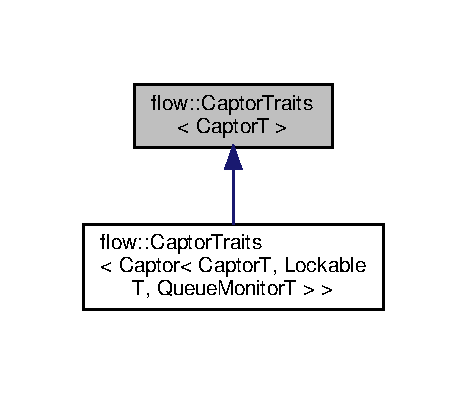
\includegraphics[width=224pt]{structflow_1_1_captor_traits__inherit__graph}
\end{center}
\end{figure}


\subsection{Detailed Description}
\subsubsection*{template$<$typename CaptorT$>$\newline
struct flow\+::\+Captor\+Traits$<$ Captor\+T $>$}

Traits struct for captor types. 

Requires\+:
\begin{DoxyItemize}
\item {\ttfamily Dispatch\+Type} \+: data dispatch object type
\item {\ttfamily Dispatch\+Container\+Type} \+: container for {\ttfamily Dispatch\+Type} {\ttfamily Dispatch\+Queue\+Monitor\+Type} \+: optional monitoring/capture preconditioning object type
\item {\ttfamily value\+\_\+type} \+: data value type
\item {\ttfamily stamp\+\_\+type} \+: sequence stamp type
\item {\ttfamily size\+\_\+type} \+: integer sizing type
\end{DoxyItemize}


\begin{DoxyTemplParams}{Template Parameters}
{\em CaptorT} & captor type with C\+R\+TP base {\ttfamily \hyperlink{classflow_1_1_captor}{Captor}} \\
\hline
\end{DoxyTemplParams}


The documentation for this struct was generated from the following file\+:\begin{DoxyCompactItemize}
\item 
flow/include/\hyperlink{captor_8h}{captor.\+h}\end{DoxyCompactItemize}

\hypertarget{structflow_1_1_captor_traits_3_01_captor_3_01_captor_t_00_01_lockable_t_00_01_queue_monitor_t_01_4_01_4}{}\section{flow\+:\+:Captor\+Traits$<$ Captor$<$ CaptorT, LockableT, Queue\+MonitorT $>$ $>$ Struct Template Reference}
\label{structflow_1_1_captor_traits_3_01_captor_3_01_captor_t_00_01_lockable_t_00_01_queue_monitor_t_01_4_01_4}\index{flow\+::\+Captor\+Traits$<$ Captor$<$ Captor\+T, Lockable\+T, Queue\+Monitor\+T $>$ $>$@{flow\+::\+Captor\+Traits$<$ Captor$<$ Captor\+T, Lockable\+T, Queue\+Monitor\+T $>$ $>$}}


Traits struct for captor types.  




{\ttfamily \#include $<$captor.\+h$>$}



Inheritance diagram for flow\+:\+:Captor\+Traits$<$ Captor$<$ CaptorT, LockableT, Queue\+MonitorT $>$ $>$\+:
\nopagebreak
\begin{figure}[H]
\begin{center}
\leavevmode
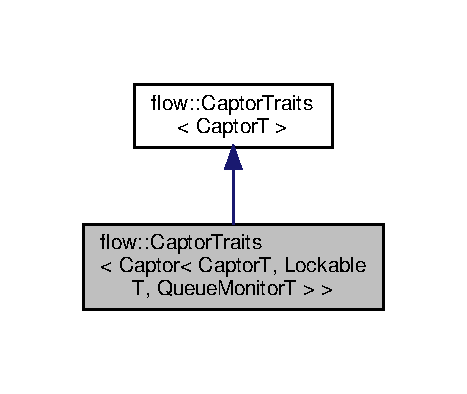
\includegraphics[width=224pt]{structflow_1_1_captor_traits_3_01_captor_3_01_captor_t_00_01_lockable_t_00_01_queue_monitor_t_01_4_01_4__inherit__graph}
\end{center}
\end{figure}


Collaboration diagram for flow\+:\+:Captor\+Traits$<$ Captor$<$ CaptorT, LockableT, Queue\+MonitorT $>$ $>$\+:
\nopagebreak
\begin{figure}[H]
\begin{center}
\leavevmode
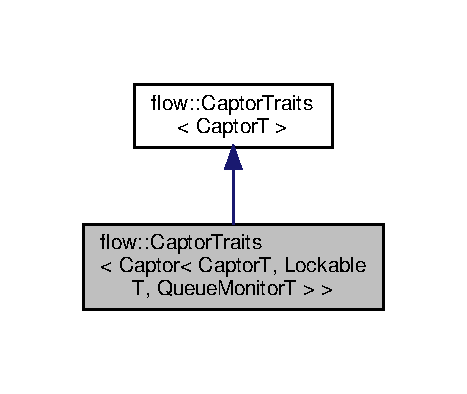
\includegraphics[width=224pt]{structflow_1_1_captor_traits_3_01_captor_3_01_captor_t_00_01_lockable_t_00_01_queue_monitor_t_01_4_01_4__coll__graph}
\end{center}
\end{figure}


\subsection{Detailed Description}
\subsubsection*{template$<$typename CaptorT, typename LockableT, typename Queue\+MonitorT$>$\newline
struct flow\+::\+Captor\+Traits$<$ Captor$<$ Captor\+T, Lockable\+T, Queue\+Monitor\+T $>$ $>$}

Traits struct for captor types. 

Requires\+:
\begin{DoxyItemize}
\item {\ttfamily Dispatch\+Type} \+: data dispatch object type
\item {\ttfamily Dispatch\+Container\+Type} \+: container for {\ttfamily Dispatch\+Type} {\ttfamily Dispatch\+Queue\+Monitor\+Type} \+: optional monitoring/capture preconditioning object type
\item {\ttfamily value\+\_\+type} \+: data value type
\item {\ttfamily stamp\+\_\+type} \+: sequence stamp type
\item {\ttfamily size\+\_\+type} \+: integer sizing type
\end{DoxyItemize}


\begin{DoxyTemplParams}{Template Parameters}
{\em CaptorT} & captor type with C\+R\+TP base {\ttfamily \hyperlink{classflow_1_1_captor}{Captor}}\\
\hline
{\em PolicyT} & C\+R\+T\+P-\/derived captor with specialized capture policy \\
\hline
\end{DoxyTemplParams}


The documentation for this struct was generated from the following file\+:\begin{DoxyCompactItemize}
\item 
flow/include/\hyperlink{captor_8h}{captor.\+h}\end{DoxyCompactItemize}

\hypertarget{structflow_1_1_captor_traits_3_01driver_1_1_batch_3_01_dispatch_t_00_01_lock_policy_t_00_01_contfc7418d386a7a1cb1fa7e6bb1299634a}{}\section{flow\+:\+:Captor\+Traits$<$ driver\+:\+:Batch$<$ DispatchT, Lock\+PolicyT, ContainerT, Queue\+MonitorT $>$ $>$ Struct Template Reference}
\label{structflow_1_1_captor_traits_3_01driver_1_1_batch_3_01_dispatch_t_00_01_lock_policy_t_00_01_contfc7418d386a7a1cb1fa7e6bb1299634a}\index{flow\+::\+Captor\+Traits$<$ driver\+::\+Batch$<$ Dispatch\+T, Lock\+Policy\+T, Container\+T, Queue\+Monitor\+T $>$ $>$@{flow\+::\+Captor\+Traits$<$ driver\+::\+Batch$<$ Dispatch\+T, Lock\+Policy\+T, Container\+T, Queue\+Monitor\+T $>$ $>$}}


Traits struct for captor types.  




{\ttfamily \#include $<$batch.\+h$>$}



Inheritance diagram for flow\+:\+:Captor\+Traits$<$ driver\+:\+:Batch$<$ DispatchT, Lock\+PolicyT, ContainerT, Queue\+MonitorT $>$ $>$\+:
\nopagebreak
\begin{figure}[H]
\begin{center}
\leavevmode
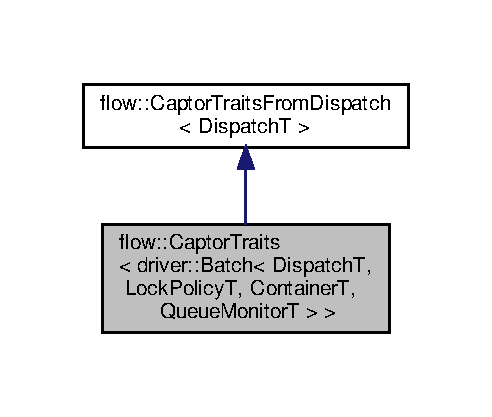
\includegraphics[width=236pt]{structflow_1_1_captor_traits_3_01driver_1_1_batch_3_01_dispatch_t_00_01_lock_policy_t_00_01_conta1d2ff9022bea6a3d1378bf812e8661a}
\end{center}
\end{figure}


Collaboration diagram for flow\+:\+:Captor\+Traits$<$ driver\+:\+:Batch$<$ DispatchT, Lock\+PolicyT, ContainerT, Queue\+MonitorT $>$ $>$\+:
\nopagebreak
\begin{figure}[H]
\begin{center}
\leavevmode
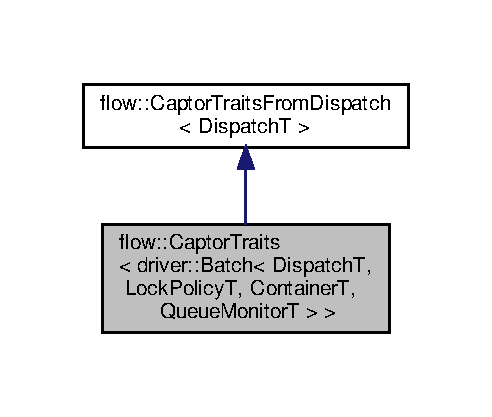
\includegraphics[width=236pt]{structflow_1_1_captor_traits_3_01driver_1_1_batch_3_01_dispatch_t_00_01_lock_policy_t_00_01_cont77cc23139130d50b732209710c04f40a}
\end{center}
\end{figure}
\subsection*{Public Types}
\begin{DoxyCompactItemize}
\item 
\mbox{\Hypertarget{structflow_1_1_captor_traits_3_01driver_1_1_batch_3_01_dispatch_t_00_01_lock_policy_t_00_01_contfc7418d386a7a1cb1fa7e6bb1299634a_ab12cef95f5c4442fdbfee614fcf917e1}\label{structflow_1_1_captor_traits_3_01driver_1_1_batch_3_01_dispatch_t_00_01_lock_policy_t_00_01_contfc7418d386a7a1cb1fa7e6bb1299634a_ab12cef95f5c4442fdbfee614fcf917e1}} 
using \hyperlink{structflow_1_1_captor_traits_3_01driver_1_1_batch_3_01_dispatch_t_00_01_lock_policy_t_00_01_contfc7418d386a7a1cb1fa7e6bb1299634a_ab12cef95f5c4442fdbfee614fcf917e1}{Dispatch\+Container\+Type} = ContainerT
\begin{DoxyCompactList}\small\item\em Underlying dispatch container type. \end{DoxyCompactList}\item 
\mbox{\Hypertarget{structflow_1_1_captor_traits_3_01driver_1_1_batch_3_01_dispatch_t_00_01_lock_policy_t_00_01_contfc7418d386a7a1cb1fa7e6bb1299634a_a9d69b494d9d11539f759d3d834d359ee}\label{structflow_1_1_captor_traits_3_01driver_1_1_batch_3_01_dispatch_t_00_01_lock_policy_t_00_01_contfc7418d386a7a1cb1fa7e6bb1299634a_a9d69b494d9d11539f759d3d834d359ee}} 
using \hyperlink{structflow_1_1_captor_traits_3_01driver_1_1_batch_3_01_dispatch_t_00_01_lock_policy_t_00_01_contfc7418d386a7a1cb1fa7e6bb1299634a_a9d69b494d9d11539f759d3d834d359ee}{Dispatch\+Queue\+Monitor\+Type} = Queue\+MonitorT
\begin{DoxyCompactList}\small\item\em Queue monitor type. \end{DoxyCompactList}\item 
\mbox{\Hypertarget{structflow_1_1_captor_traits_3_01driver_1_1_batch_3_01_dispatch_t_00_01_lock_policy_t_00_01_contfc7418d386a7a1cb1fa7e6bb1299634a_afdacb7efd1e83c5d2621649aeb86bf7d}\label{structflow_1_1_captor_traits_3_01driver_1_1_batch_3_01_dispatch_t_00_01_lock_policy_t_00_01_contfc7418d386a7a1cb1fa7e6bb1299634a_afdacb7efd1e83c5d2621649aeb86bf7d}} 
using \hyperlink{structflow_1_1_captor_traits_3_01driver_1_1_batch_3_01_dispatch_t_00_01_lock_policy_t_00_01_contfc7418d386a7a1cb1fa7e6bb1299634a_afdacb7efd1e83c5d2621649aeb86bf7d}{Lock\+Policy\+Type} = Lock\+PolicyT
\begin{DoxyCompactList}\small\item\em Thread locking policy type. \end{DoxyCompactList}\end{DoxyCompactItemize}
\subsection*{Static Public Attributes}
\begin{DoxyCompactItemize}
\item 
static constexpr bool \hyperlink{structflow_1_1_captor_traits_3_01driver_1_1_batch_3_01_dispatch_t_00_01_lock_policy_t_00_01_contfc7418d386a7a1cb1fa7e6bb1299634a_a363194e346e30aaba6f166e537156a82}{is\+\_\+capture\+\_\+deterministic} = true
\end{DoxyCompactItemize}


\subsection{Detailed Description}
\subsubsection*{template$<$typename DispatchT, typename Lock\+PolicyT, typename ContainerT, typename Queue\+MonitorT$>$\newline
struct flow\+::\+Captor\+Traits$<$ driver\+::\+Batch$<$ Dispatch\+T, Lock\+Policy\+T, Container\+T, Queue\+Monitor\+T $>$ $>$}

Traits struct for captor types. 

Requires\+:
\begin{DoxyItemize}
\item {\ttfamily Dispatch\+Type} \+: data dispatch object type
\item {\ttfamily Dispatch\+Container\+Type} \+: container for {\ttfamily Dispatch\+Type} {\ttfamily Dispatch\+Queue\+Monitor\+Type} \+: optional monitoring/capture preconditioning object type
\item {\ttfamily value\+\_\+type} \+: data value type
\item {\ttfamily stamp\+\_\+type} \+: sequence stamp type
\item {\ttfamily size\+\_\+type} \+: integer sizing type
\end{DoxyItemize}


\begin{DoxyTemplParams}{Template Parameters}
{\em CaptorT} & captor type with C\+R\+TP base {\ttfamily \hyperlink{classflow_1_1_captor}{Captor}}\\
\hline
{\em DispatchT} & data dispatch type \\
\hline
{\em Lock\+PolicyT} & a Basic\+Lockable (\href{https://en.cppreference.com/w/cpp/named_req/BasicLockable}{\tt https\+://en.\+cppreference.\+com/w/cpp/named\+\_\+req/\+Basic\+Lockable}) object or \hyperlink{structflow_1_1_no_lock}{No\+Lock} or \hyperlink{structflow_1_1_polling_lock}{Polling\+Lock} \\
\hline
{\em ContainerT} & underlying {\ttfamily DispatchT} container type \\
\hline
{\em Queue\+MonitorT} & object used to monitor queue state on each insertion \\
\hline
\end{DoxyTemplParams}


\subsection{Member Data Documentation}
\mbox{\Hypertarget{structflow_1_1_captor_traits_3_01driver_1_1_batch_3_01_dispatch_t_00_01_lock_policy_t_00_01_contfc7418d386a7a1cb1fa7e6bb1299634a_a363194e346e30aaba6f166e537156a82}\label{structflow_1_1_captor_traits_3_01driver_1_1_batch_3_01_dispatch_t_00_01_lock_policy_t_00_01_contfc7418d386a7a1cb1fa7e6bb1299634a_a363194e346e30aaba6f166e537156a82}} 
\index{flow\+::\+Captor\+Traits$<$ driver\+::\+Batch$<$ Dispatch\+T, Lock\+Policy\+T, Container\+T, Queue\+Monitor\+T $>$ $>$@{flow\+::\+Captor\+Traits$<$ driver\+::\+Batch$<$ Dispatch\+T, Lock\+Policy\+T, Container\+T, Queue\+Monitor\+T $>$ $>$}!is\+\_\+capture\+\_\+deterministic@{is\+\_\+capture\+\_\+deterministic}}
\index{is\+\_\+capture\+\_\+deterministic@{is\+\_\+capture\+\_\+deterministic}!flow\+::\+Captor\+Traits$<$ driver\+::\+Batch$<$ Dispatch\+T, Lock\+Policy\+T, Container\+T, Queue\+Monitor\+T $>$ $>$@{flow\+::\+Captor\+Traits$<$ driver\+::\+Batch$<$ Dispatch\+T, Lock\+Policy\+T, Container\+T, Queue\+Monitor\+T $>$ $>$}}
\subsubsection{\texorpdfstring{is\+\_\+capture\+\_\+deterministic}{is\_capture\_deterministic}}
{\footnotesize\ttfamily template$<$typename DispatchT , typename Lock\+PolicyT , typename ContainerT , typename Queue\+MonitorT $>$ \\
constexpr bool \hyperlink{structflow_1_1_captor_traits}{flow\+::\+Captor\+Traits}$<$ \hyperlink{classflow_1_1driver_1_1_batch}{driver\+::\+Batch}$<$ DispatchT, Lock\+PolicyT, ContainerT, Queue\+MonitorT $>$ $>$\+::is\+\_\+capture\+\_\+deterministic = true\hspace{0.3cm}{\ttfamily [static]}}

Indicates that data from this captor will always be captured deterministically, so long as data injection is monotonically sequenced 

The documentation for this struct was generated from the following file\+:\begin{DoxyCompactItemize}
\item 
flow/include/driver/\hyperlink{batch_8h}{batch.\+h}\end{DoxyCompactItemize}

\hypertarget{structflow_1_1_captor_traits_3_01driver_1_1_chunk_3_01_dispatch_t_00_01_lock_policy_t_00_01_contf25136d799b84e6e744301cf371fdfc2}{}\section{flow\+:\+:Captor\+Traits$<$ driver\+:\+:Chunk$<$ DispatchT, Lock\+PolicyT, ContainerT, Queue\+MonitorT $>$ $>$ Struct Template Reference}
\label{structflow_1_1_captor_traits_3_01driver_1_1_chunk_3_01_dispatch_t_00_01_lock_policy_t_00_01_contf25136d799b84e6e744301cf371fdfc2}\index{flow\+::\+Captor\+Traits$<$ driver\+::\+Chunk$<$ Dispatch\+T, Lock\+Policy\+T, Container\+T, Queue\+Monitor\+T $>$ $>$@{flow\+::\+Captor\+Traits$<$ driver\+::\+Chunk$<$ Dispatch\+T, Lock\+Policy\+T, Container\+T, Queue\+Monitor\+T $>$ $>$}}


Traits struct for captor types.  




{\ttfamily \#include $<$chunk.\+h$>$}



Inheritance diagram for flow\+:\+:Captor\+Traits$<$ driver\+:\+:Chunk$<$ DispatchT, Lock\+PolicyT, ContainerT, Queue\+MonitorT $>$ $>$\+:
\nopagebreak
\begin{figure}[H]
\begin{center}
\leavevmode
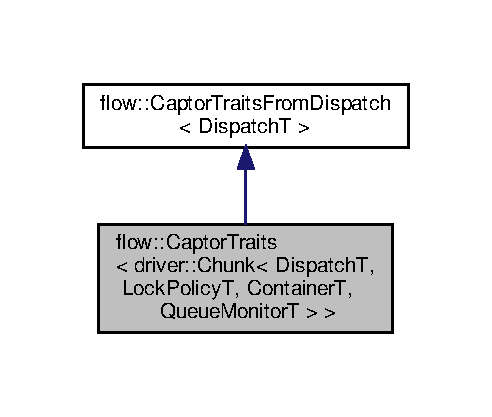
\includegraphics[width=236pt]{structflow_1_1_captor_traits_3_01driver_1_1_chunk_3_01_dispatch_t_00_01_lock_policy_t_00_01_contd827df6a40b2e91b19343856540a74d5}
\end{center}
\end{figure}


Collaboration diagram for flow\+:\+:Captor\+Traits$<$ driver\+:\+:Chunk$<$ DispatchT, Lock\+PolicyT, ContainerT, Queue\+MonitorT $>$ $>$\+:
\nopagebreak
\begin{figure}[H]
\begin{center}
\leavevmode
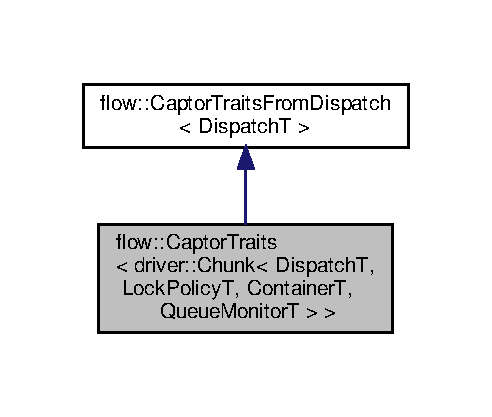
\includegraphics[width=236pt]{structflow_1_1_captor_traits_3_01driver_1_1_chunk_3_01_dispatch_t_00_01_lock_policy_t_00_01_cont659f81f1f0b31165d4c94f5bd0a0144c}
\end{center}
\end{figure}
\subsection*{Public Types}
\begin{DoxyCompactItemize}
\item 
\mbox{\Hypertarget{structflow_1_1_captor_traits_3_01driver_1_1_chunk_3_01_dispatch_t_00_01_lock_policy_t_00_01_contf25136d799b84e6e744301cf371fdfc2_a637f1f6856c95432d0af46e932a7cd89}\label{structflow_1_1_captor_traits_3_01driver_1_1_chunk_3_01_dispatch_t_00_01_lock_policy_t_00_01_contf25136d799b84e6e744301cf371fdfc2_a637f1f6856c95432d0af46e932a7cd89}} 
using \hyperlink{structflow_1_1_captor_traits_3_01driver_1_1_chunk_3_01_dispatch_t_00_01_lock_policy_t_00_01_contf25136d799b84e6e744301cf371fdfc2_a637f1f6856c95432d0af46e932a7cd89}{Dispatch\+Container\+Type} = ContainerT
\begin{DoxyCompactList}\small\item\em Underlying dispatch container type. \end{DoxyCompactList}\item 
\mbox{\Hypertarget{structflow_1_1_captor_traits_3_01driver_1_1_chunk_3_01_dispatch_t_00_01_lock_policy_t_00_01_contf25136d799b84e6e744301cf371fdfc2_ae368577509b5c8658cb849260c0f47b6}\label{structflow_1_1_captor_traits_3_01driver_1_1_chunk_3_01_dispatch_t_00_01_lock_policy_t_00_01_contf25136d799b84e6e744301cf371fdfc2_ae368577509b5c8658cb849260c0f47b6}} 
using \hyperlink{structflow_1_1_captor_traits_3_01driver_1_1_chunk_3_01_dispatch_t_00_01_lock_policy_t_00_01_contf25136d799b84e6e744301cf371fdfc2_ae368577509b5c8658cb849260c0f47b6}{Dispatch\+Queue\+Monitor\+Type} = \hyperlink{structflow_1_1_default_dispatch_queue_monitor}{Default\+Dispatch\+Queue\+Monitor}
\begin{DoxyCompactList}\small\item\em Queue monitor type. \end{DoxyCompactList}\item 
\mbox{\Hypertarget{structflow_1_1_captor_traits_3_01driver_1_1_chunk_3_01_dispatch_t_00_01_lock_policy_t_00_01_contf25136d799b84e6e744301cf371fdfc2_acc49027a34bba9309e8875bc25001854}\label{structflow_1_1_captor_traits_3_01driver_1_1_chunk_3_01_dispatch_t_00_01_lock_policy_t_00_01_contf25136d799b84e6e744301cf371fdfc2_acc49027a34bba9309e8875bc25001854}} 
using \hyperlink{structflow_1_1_captor_traits_3_01driver_1_1_chunk_3_01_dispatch_t_00_01_lock_policy_t_00_01_contf25136d799b84e6e744301cf371fdfc2_acc49027a34bba9309e8875bc25001854}{Lock\+Policy\+Type} = Lock\+PolicyT
\begin{DoxyCompactList}\small\item\em Thread locking policy type. \end{DoxyCompactList}\end{DoxyCompactItemize}
\subsection*{Static Public Attributes}
\begin{DoxyCompactItemize}
\item 
static constexpr bool \hyperlink{structflow_1_1_captor_traits_3_01driver_1_1_chunk_3_01_dispatch_t_00_01_lock_policy_t_00_01_contf25136d799b84e6e744301cf371fdfc2_ada5c859ac589ebdf628e3f687e43e188}{is\+\_\+capture\+\_\+deterministic} = true
\end{DoxyCompactItemize}


\subsection{Detailed Description}
\subsubsection*{template$<$typename DispatchT, typename Lock\+PolicyT, typename ContainerT, typename Queue\+MonitorT$>$\newline
struct flow\+::\+Captor\+Traits$<$ driver\+::\+Chunk$<$ Dispatch\+T, Lock\+Policy\+T, Container\+T, Queue\+Monitor\+T $>$ $>$}

Traits struct for captor types. 

Requires\+:
\begin{DoxyItemize}
\item {\ttfamily Dispatch\+Type} \+: data dispatch object type
\item {\ttfamily Dispatch\+Container\+Type} \+: container for {\ttfamily Dispatch\+Type} {\ttfamily Dispatch\+Queue\+Monitor\+Type} \+: optional monitoring/capture preconditioning object type
\item {\ttfamily value\+\_\+type} \+: data value type
\item {\ttfamily stamp\+\_\+type} \+: sequence stamp type
\item {\ttfamily size\+\_\+type} \+: integer sizing type
\end{DoxyItemize}


\begin{DoxyTemplParams}{Template Parameters}
{\em CaptorT} & captor type with C\+R\+TP base {\ttfamily \hyperlink{classflow_1_1_captor}{Captor}}\\
\hline
{\em DispatchT} & data dispatch type \\
\hline
{\em Lock\+PolicyT} & a Basic\+Lockable (\href{https://en.cppreference.com/w/cpp/named_req/BasicLockable}{\tt https\+://en.\+cppreference.\+com/w/cpp/named\+\_\+req/\+Basic\+Lockable}) object or \hyperlink{structflow_1_1_no_lock}{No\+Lock} or \hyperlink{structflow_1_1_polling_lock}{Polling\+Lock} \\
\hline
{\em ContainerT} & underlying {\ttfamily DispatchT} container type \\
\hline
{\em Queue\+MonitorT} & object used to monitor queue state on each insertion \\
\hline
\end{DoxyTemplParams}


\subsection{Member Data Documentation}
\mbox{\Hypertarget{structflow_1_1_captor_traits_3_01driver_1_1_chunk_3_01_dispatch_t_00_01_lock_policy_t_00_01_contf25136d799b84e6e744301cf371fdfc2_ada5c859ac589ebdf628e3f687e43e188}\label{structflow_1_1_captor_traits_3_01driver_1_1_chunk_3_01_dispatch_t_00_01_lock_policy_t_00_01_contf25136d799b84e6e744301cf371fdfc2_ada5c859ac589ebdf628e3f687e43e188}} 
\index{flow\+::\+Captor\+Traits$<$ driver\+::\+Chunk$<$ Dispatch\+T, Lock\+Policy\+T, Container\+T, Queue\+Monitor\+T $>$ $>$@{flow\+::\+Captor\+Traits$<$ driver\+::\+Chunk$<$ Dispatch\+T, Lock\+Policy\+T, Container\+T, Queue\+Monitor\+T $>$ $>$}!is\+\_\+capture\+\_\+deterministic@{is\+\_\+capture\+\_\+deterministic}}
\index{is\+\_\+capture\+\_\+deterministic@{is\+\_\+capture\+\_\+deterministic}!flow\+::\+Captor\+Traits$<$ driver\+::\+Chunk$<$ Dispatch\+T, Lock\+Policy\+T, Container\+T, Queue\+Monitor\+T $>$ $>$@{flow\+::\+Captor\+Traits$<$ driver\+::\+Chunk$<$ Dispatch\+T, Lock\+Policy\+T, Container\+T, Queue\+Monitor\+T $>$ $>$}}
\subsubsection{\texorpdfstring{is\+\_\+capture\+\_\+deterministic}{is\_capture\_deterministic}}
{\footnotesize\ttfamily template$<$typename DispatchT , typename Lock\+PolicyT , typename ContainerT , typename Queue\+MonitorT $>$ \\
constexpr bool \hyperlink{structflow_1_1_captor_traits}{flow\+::\+Captor\+Traits}$<$ \hyperlink{classflow_1_1driver_1_1_chunk}{driver\+::\+Chunk}$<$ DispatchT, Lock\+PolicyT, ContainerT, Queue\+MonitorT $>$ $>$\+::is\+\_\+capture\+\_\+deterministic = true\hspace{0.3cm}{\ttfamily [static]}}

Indicates that data from this captor will always be captured deterministically, so long as data injection is monotonically sequenced 

The documentation for this struct was generated from the following file\+:\begin{DoxyCompactItemize}
\item 
flow/include/driver/chunk.\+h\end{DoxyCompactItemize}

\hypertarget{structflow_1_1_captor_traits_3_01driver_1_1_next_3_01_dispatch_t_00_01_lock_policy_t_00_01_contacacf8f9584444cf22afe31e8b706b576}{}\section{flow\+:\+:Captor\+Traits$<$ driver\+:\+:Next$<$ DispatchT, Lock\+PolicyT, ContainerT, Queue\+MonitorT $>$ $>$ Struct Template Reference}
\label{structflow_1_1_captor_traits_3_01driver_1_1_next_3_01_dispatch_t_00_01_lock_policy_t_00_01_contacacf8f9584444cf22afe31e8b706b576}\index{flow\+::\+Captor\+Traits$<$ driver\+::\+Next$<$ Dispatch\+T, Lock\+Policy\+T, Container\+T, Queue\+Monitor\+T $>$ $>$@{flow\+::\+Captor\+Traits$<$ driver\+::\+Next$<$ Dispatch\+T, Lock\+Policy\+T, Container\+T, Queue\+Monitor\+T $>$ $>$}}


Traits struct for captor types.  




{\ttfamily \#include $<$next.\+h$>$}



Inheritance diagram for flow\+:\+:Captor\+Traits$<$ driver\+:\+:Next$<$ DispatchT, Lock\+PolicyT, ContainerT, Queue\+MonitorT $>$ $>$\+:
\nopagebreak
\begin{figure}[H]
\begin{center}
\leavevmode
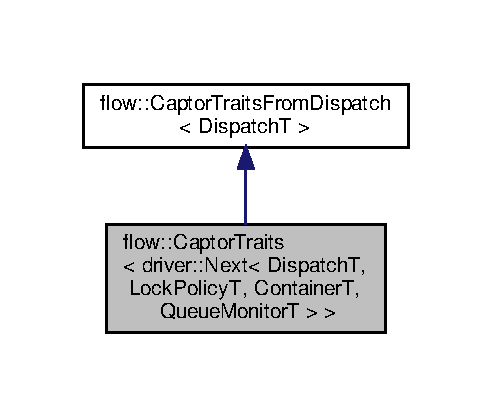
\includegraphics[width=236pt]{structflow_1_1_captor_traits_3_01driver_1_1_next_3_01_dispatch_t_00_01_lock_policy_t_00_01_contadec8c8f1b5967280a88167134136c691}
\end{center}
\end{figure}


Collaboration diagram for flow\+:\+:Captor\+Traits$<$ driver\+:\+:Next$<$ DispatchT, Lock\+PolicyT, ContainerT, Queue\+MonitorT $>$ $>$\+:
\nopagebreak
\begin{figure}[H]
\begin{center}
\leavevmode
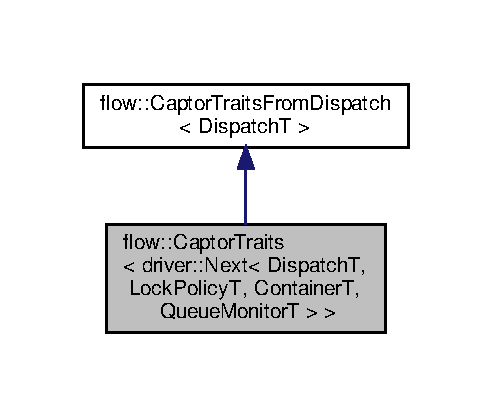
\includegraphics[width=236pt]{structflow_1_1_captor_traits_3_01driver_1_1_next_3_01_dispatch_t_00_01_lock_policy_t_00_01_conta7b28c4337d688b572dfca57dcc4eb0e7}
\end{center}
\end{figure}
\subsection*{Public Types}
\begin{DoxyCompactItemize}
\item 
\mbox{\Hypertarget{structflow_1_1_captor_traits_3_01driver_1_1_next_3_01_dispatch_t_00_01_lock_policy_t_00_01_contacacf8f9584444cf22afe31e8b706b576_a02a8c83ec97c18fb7d98386e063a5915}\label{structflow_1_1_captor_traits_3_01driver_1_1_next_3_01_dispatch_t_00_01_lock_policy_t_00_01_contacacf8f9584444cf22afe31e8b706b576_a02a8c83ec97c18fb7d98386e063a5915}} 
using \hyperlink{structflow_1_1_captor_traits_3_01driver_1_1_next_3_01_dispatch_t_00_01_lock_policy_t_00_01_contacacf8f9584444cf22afe31e8b706b576_a02a8c83ec97c18fb7d98386e063a5915}{Dispatch\+Container\+Type} = ContainerT
\begin{DoxyCompactList}\small\item\em Underlying dispatch container type. \end{DoxyCompactList}\item 
\mbox{\Hypertarget{structflow_1_1_captor_traits_3_01driver_1_1_next_3_01_dispatch_t_00_01_lock_policy_t_00_01_contacacf8f9584444cf22afe31e8b706b576_aed990ea0a8dceaf3fb24ff87179eeaed}\label{structflow_1_1_captor_traits_3_01driver_1_1_next_3_01_dispatch_t_00_01_lock_policy_t_00_01_contacacf8f9584444cf22afe31e8b706b576_aed990ea0a8dceaf3fb24ff87179eeaed}} 
using \hyperlink{structflow_1_1_captor_traits_3_01driver_1_1_next_3_01_dispatch_t_00_01_lock_policy_t_00_01_contacacf8f9584444cf22afe31e8b706b576_aed990ea0a8dceaf3fb24ff87179eeaed}{Dispatch\+Queue\+Monitor\+Type} = Queue\+MonitorT
\begin{DoxyCompactList}\small\item\em Queue monitor type. \end{DoxyCompactList}\item 
\mbox{\Hypertarget{structflow_1_1_captor_traits_3_01driver_1_1_next_3_01_dispatch_t_00_01_lock_policy_t_00_01_contacacf8f9584444cf22afe31e8b706b576_a4cc35f0f8fa9af0ce1e2db70e874338e}\label{structflow_1_1_captor_traits_3_01driver_1_1_next_3_01_dispatch_t_00_01_lock_policy_t_00_01_contacacf8f9584444cf22afe31e8b706b576_a4cc35f0f8fa9af0ce1e2db70e874338e}} 
using \hyperlink{structflow_1_1_captor_traits_3_01driver_1_1_next_3_01_dispatch_t_00_01_lock_policy_t_00_01_contacacf8f9584444cf22afe31e8b706b576_a4cc35f0f8fa9af0ce1e2db70e874338e}{Lock\+Policy\+Type} = Lock\+PolicyT
\begin{DoxyCompactList}\small\item\em Thread locking policy type. \end{DoxyCompactList}\end{DoxyCompactItemize}
\subsection*{Static Public Attributes}
\begin{DoxyCompactItemize}
\item 
static constexpr bool \hyperlink{structflow_1_1_captor_traits_3_01driver_1_1_next_3_01_dispatch_t_00_01_lock_policy_t_00_01_contacacf8f9584444cf22afe31e8b706b576_a4cdc11c4e961fc4e0d763cbb209d93eb}{is\+\_\+capture\+\_\+deterministic} = true
\end{DoxyCompactItemize}


\subsection{Detailed Description}
\subsubsection*{template$<$typename DispatchT, typename Lock\+PolicyT, typename ContainerT, typename Queue\+MonitorT$>$\newline
struct flow\+::\+Captor\+Traits$<$ driver\+::\+Next$<$ Dispatch\+T, Lock\+Policy\+T, Container\+T, Queue\+Monitor\+T $>$ $>$}

Traits struct for captor types. 

Requires\+:
\begin{DoxyItemize}
\item {\ttfamily Dispatch\+Type} \+: data dispatch object type
\item {\ttfamily Dispatch\+Container\+Type} \+: container for {\ttfamily Dispatch\+Type} {\ttfamily Dispatch\+Queue\+Monitor\+Type} \+: optional monitoring/capture preconditioning object type
\item {\ttfamily value\+\_\+type} \+: data value type
\item {\ttfamily stamp\+\_\+type} \+: sequence stamp type
\item {\ttfamily size\+\_\+type} \+: integer sizing type
\end{DoxyItemize}


\begin{DoxyTemplParams}{Template Parameters}
{\em CaptorT} & captor type with C\+R\+TP base {\ttfamily \hyperlink{classflow_1_1_captor}{Captor}}\\
\hline
{\em DispatchT} & data dispatch type \\
\hline
{\em Lock\+PolicyT} & a Basic\+Lockable (\href{https://en.cppreference.com/w/cpp/named_req/BasicLockable}{\tt https\+://en.\+cppreference.\+com/w/cpp/named\+\_\+req/\+Basic\+Lockable}) object or \hyperlink{structflow_1_1_no_lock}{No\+Lock} or \hyperlink{structflow_1_1_polling_lock}{Polling\+Lock} \\
\hline
{\em ContainerT} & underlying {\ttfamily DispatchT} container type \\
\hline
{\em Queue\+MonitorT} & object used to monitor queue state on each insertion \\
\hline
\end{DoxyTemplParams}


\subsection{Member Data Documentation}
\mbox{\Hypertarget{structflow_1_1_captor_traits_3_01driver_1_1_next_3_01_dispatch_t_00_01_lock_policy_t_00_01_contacacf8f9584444cf22afe31e8b706b576_a4cdc11c4e961fc4e0d763cbb209d93eb}\label{structflow_1_1_captor_traits_3_01driver_1_1_next_3_01_dispatch_t_00_01_lock_policy_t_00_01_contacacf8f9584444cf22afe31e8b706b576_a4cdc11c4e961fc4e0d763cbb209d93eb}} 
\index{flow\+::\+Captor\+Traits$<$ driver\+::\+Next$<$ Dispatch\+T, Lock\+Policy\+T, Container\+T, Queue\+Monitor\+T $>$ $>$@{flow\+::\+Captor\+Traits$<$ driver\+::\+Next$<$ Dispatch\+T, Lock\+Policy\+T, Container\+T, Queue\+Monitor\+T $>$ $>$}!is\+\_\+capture\+\_\+deterministic@{is\+\_\+capture\+\_\+deterministic}}
\index{is\+\_\+capture\+\_\+deterministic@{is\+\_\+capture\+\_\+deterministic}!flow\+::\+Captor\+Traits$<$ driver\+::\+Next$<$ Dispatch\+T, Lock\+Policy\+T, Container\+T, Queue\+Monitor\+T $>$ $>$@{flow\+::\+Captor\+Traits$<$ driver\+::\+Next$<$ Dispatch\+T, Lock\+Policy\+T, Container\+T, Queue\+Monitor\+T $>$ $>$}}
\subsubsection{\texorpdfstring{is\+\_\+capture\+\_\+deterministic}{is\_capture\_deterministic}}
{\footnotesize\ttfamily template$<$typename DispatchT , typename Lock\+PolicyT , typename ContainerT , typename Queue\+MonitorT $>$ \\
constexpr bool \hyperlink{structflow_1_1_captor_traits}{flow\+::\+Captor\+Traits}$<$ \hyperlink{classflow_1_1driver_1_1_next}{driver\+::\+Next}$<$ DispatchT, Lock\+PolicyT, ContainerT, Queue\+MonitorT $>$ $>$\+::is\+\_\+capture\+\_\+deterministic = true\hspace{0.3cm}{\ttfamily [static]}}

Indicates that data from this captor will always be captured deterministically, so long as data injection is monotonically sequenced 

The documentation for this struct was generated from the following file\+:\begin{DoxyCompactItemize}
\item 
flow/include/driver/\hyperlink{next_8h}{next.\+h}\end{DoxyCompactItemize}

\hypertarget{structflow_1_1_captor_traits_3_01driver_1_1_throttled_3_01_dispatch_t_00_01_lock_policy_t_00_01_a55b272e8914e815b1e61540d6e370f1}{}\section{flow\+:\+:Captor\+Traits$<$ driver\+:\+:Throttled$<$ DispatchT, Lock\+PolicyT, ContainerT, Queue\+MonitorT $>$ $>$ Struct Template Reference}
\label{structflow_1_1_captor_traits_3_01driver_1_1_throttled_3_01_dispatch_t_00_01_lock_policy_t_00_01_a55b272e8914e815b1e61540d6e370f1}\index{flow\+::\+Captor\+Traits$<$ driver\+::\+Throttled$<$ Dispatch\+T, Lock\+Policy\+T, Container\+T, Queue\+Monitor\+T $>$ $>$@{flow\+::\+Captor\+Traits$<$ driver\+::\+Throttled$<$ Dispatch\+T, Lock\+Policy\+T, Container\+T, Queue\+Monitor\+T $>$ $>$}}


Traits struct for captor types.  




{\ttfamily \#include $<$throttled.\+h$>$}



Inheritance diagram for flow\+:\+:Captor\+Traits$<$ driver\+:\+:Throttled$<$ DispatchT, Lock\+PolicyT, ContainerT, Queue\+MonitorT $>$ $>$\+:
\nopagebreak
\begin{figure}[H]
\begin{center}
\leavevmode
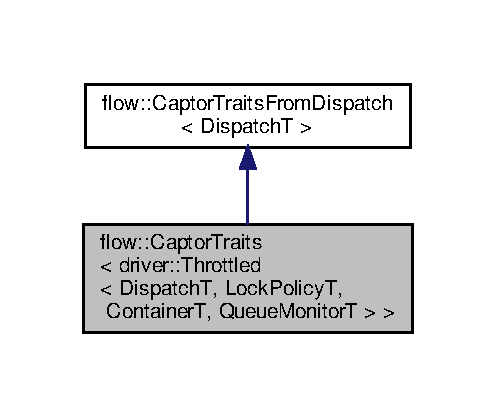
\includegraphics[width=238pt]{structflow_1_1_captor_traits_3_01driver_1_1_throttled_3_01_dispatch_t_00_01_lock_policy_t_00_01_14c144804262ca375e62b50400bd9ca4}
\end{center}
\end{figure}


Collaboration diagram for flow\+:\+:Captor\+Traits$<$ driver\+:\+:Throttled$<$ DispatchT, Lock\+PolicyT, ContainerT, Queue\+MonitorT $>$ $>$\+:
\nopagebreak
\begin{figure}[H]
\begin{center}
\leavevmode
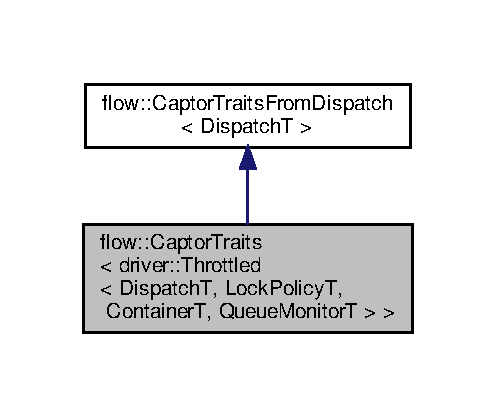
\includegraphics[width=238pt]{structflow_1_1_captor_traits_3_01driver_1_1_throttled_3_01_dispatch_t_00_01_lock_policy_t_00_01_85def682def35b36744c18cf6f6e3210}
\end{center}
\end{figure}
\subsection*{Public Types}
\begin{DoxyCompactItemize}
\item 
\mbox{\Hypertarget{structflow_1_1_captor_traits_3_01driver_1_1_throttled_3_01_dispatch_t_00_01_lock_policy_t_00_01_a55b272e8914e815b1e61540d6e370f1_a4ccbeb5b2a25d51a25a8489fd330a01b}\label{structflow_1_1_captor_traits_3_01driver_1_1_throttled_3_01_dispatch_t_00_01_lock_policy_t_00_01_a55b272e8914e815b1e61540d6e370f1_a4ccbeb5b2a25d51a25a8489fd330a01b}} 
using \hyperlink{structflow_1_1_captor_traits_3_01driver_1_1_throttled_3_01_dispatch_t_00_01_lock_policy_t_00_01_a55b272e8914e815b1e61540d6e370f1_a4ccbeb5b2a25d51a25a8489fd330a01b}{Dispatch\+Container\+Type} = ContainerT
\begin{DoxyCompactList}\small\item\em Underlying dispatch container type. \end{DoxyCompactList}\item 
\mbox{\Hypertarget{structflow_1_1_captor_traits_3_01driver_1_1_throttled_3_01_dispatch_t_00_01_lock_policy_t_00_01_a55b272e8914e815b1e61540d6e370f1_a7386696d4d65327741854e6dd6f38ff0}\label{structflow_1_1_captor_traits_3_01driver_1_1_throttled_3_01_dispatch_t_00_01_lock_policy_t_00_01_a55b272e8914e815b1e61540d6e370f1_a7386696d4d65327741854e6dd6f38ff0}} 
using \hyperlink{structflow_1_1_captor_traits_3_01driver_1_1_throttled_3_01_dispatch_t_00_01_lock_policy_t_00_01_a55b272e8914e815b1e61540d6e370f1_a7386696d4d65327741854e6dd6f38ff0}{Dispatch\+Queue\+Monitor\+Type} = Queue\+MonitorT
\begin{DoxyCompactList}\small\item\em Queue monitor type. \end{DoxyCompactList}\item 
\mbox{\Hypertarget{structflow_1_1_captor_traits_3_01driver_1_1_throttled_3_01_dispatch_t_00_01_lock_policy_t_00_01_a55b272e8914e815b1e61540d6e370f1_a2cb2dc4ee8e2cc118ca3bbea5df4462f}\label{structflow_1_1_captor_traits_3_01driver_1_1_throttled_3_01_dispatch_t_00_01_lock_policy_t_00_01_a55b272e8914e815b1e61540d6e370f1_a2cb2dc4ee8e2cc118ca3bbea5df4462f}} 
using \hyperlink{structflow_1_1_captor_traits_3_01driver_1_1_throttled_3_01_dispatch_t_00_01_lock_policy_t_00_01_a55b272e8914e815b1e61540d6e370f1_a2cb2dc4ee8e2cc118ca3bbea5df4462f}{Lock\+Policy\+Type} = Lock\+PolicyT
\begin{DoxyCompactList}\small\item\em Thread locking policy type. \end{DoxyCompactList}\end{DoxyCompactItemize}
\subsection*{Static Public Attributes}
\begin{DoxyCompactItemize}
\item 
static constexpr bool \hyperlink{structflow_1_1_captor_traits_3_01driver_1_1_throttled_3_01_dispatch_t_00_01_lock_policy_t_00_01_a55b272e8914e815b1e61540d6e370f1_a9f7dab8a0536fda23364cc6f86e8fc74}{is\+\_\+capture\+\_\+deterministic} = true
\end{DoxyCompactItemize}


\subsection{Detailed Description}
\subsubsection*{template$<$typename DispatchT, typename Lock\+PolicyT, typename ContainerT, typename Queue\+MonitorT$>$\newline
struct flow\+::\+Captor\+Traits$<$ driver\+::\+Throttled$<$ Dispatch\+T, Lock\+Policy\+T, Container\+T, Queue\+Monitor\+T $>$ $>$}

Traits struct for captor types. 

Requires\+:
\begin{DoxyItemize}
\item {\ttfamily Dispatch\+Type} \+: data dispatch object type
\item {\ttfamily Dispatch\+Container\+Type} \+: container for {\ttfamily Dispatch\+Type} {\ttfamily Dispatch\+Queue\+Monitor\+Type} \+: optional monitoring/capture preconditioning object type
\item {\ttfamily value\+\_\+type} \+: data value type
\item {\ttfamily stamp\+\_\+type} \+: sequence stamp type
\item {\ttfamily size\+\_\+type} \+: integer sizing type
\end{DoxyItemize}


\begin{DoxyTemplParams}{Template Parameters}
{\em CaptorT} & captor type with C\+R\+TP base {\ttfamily \hyperlink{classflow_1_1_captor}{Captor}}\\
\hline
{\em DispatchT} & data dispatch type \\
\hline
{\em Lock\+PolicyT} & a Basic\+Lockable (\href{https://en.cppreference.com/w/cpp/named_req/BasicLockable}{\tt https\+://en.\+cppreference.\+com/w/cpp/named\+\_\+req/\+Basic\+Lockable}) object or \hyperlink{structflow_1_1_no_lock}{No\+Lock} or \hyperlink{structflow_1_1_polling_lock}{Polling\+Lock} \\
\hline
{\em ContainerT} & underlying {\ttfamily DispatchT} container type \\
\hline
{\em Queue\+MonitorT} & object used to monitor queue state on each insertion \\
\hline
\end{DoxyTemplParams}


\subsection{Member Data Documentation}
\mbox{\Hypertarget{structflow_1_1_captor_traits_3_01driver_1_1_throttled_3_01_dispatch_t_00_01_lock_policy_t_00_01_a55b272e8914e815b1e61540d6e370f1_a9f7dab8a0536fda23364cc6f86e8fc74}\label{structflow_1_1_captor_traits_3_01driver_1_1_throttled_3_01_dispatch_t_00_01_lock_policy_t_00_01_a55b272e8914e815b1e61540d6e370f1_a9f7dab8a0536fda23364cc6f86e8fc74}} 
\index{flow\+::\+Captor\+Traits$<$ driver\+::\+Throttled$<$ Dispatch\+T, Lock\+Policy\+T, Container\+T, Queue\+Monitor\+T $>$ $>$@{flow\+::\+Captor\+Traits$<$ driver\+::\+Throttled$<$ Dispatch\+T, Lock\+Policy\+T, Container\+T, Queue\+Monitor\+T $>$ $>$}!is\+\_\+capture\+\_\+deterministic@{is\+\_\+capture\+\_\+deterministic}}
\index{is\+\_\+capture\+\_\+deterministic@{is\+\_\+capture\+\_\+deterministic}!flow\+::\+Captor\+Traits$<$ driver\+::\+Throttled$<$ Dispatch\+T, Lock\+Policy\+T, Container\+T, Queue\+Monitor\+T $>$ $>$@{flow\+::\+Captor\+Traits$<$ driver\+::\+Throttled$<$ Dispatch\+T, Lock\+Policy\+T, Container\+T, Queue\+Monitor\+T $>$ $>$}}
\subsubsection{\texorpdfstring{is\+\_\+capture\+\_\+deterministic}{is\_capture\_deterministic}}
{\footnotesize\ttfamily template$<$typename DispatchT , typename Lock\+PolicyT , typename ContainerT , typename Queue\+MonitorT $>$ \\
constexpr bool \hyperlink{structflow_1_1_captor_traits}{flow\+::\+Captor\+Traits}$<$ \hyperlink{classflow_1_1driver_1_1_throttled}{driver\+::\+Throttled}$<$ DispatchT, Lock\+PolicyT, ContainerT, Queue\+MonitorT $>$ $>$\+::is\+\_\+capture\+\_\+deterministic = true\hspace{0.3cm}{\ttfamily [static]}}

Indicates that data from this captor will always be captured deterministically, so long as data injection is monotonically sequenced 

The documentation for this struct was generated from the following file\+:\begin{DoxyCompactItemize}
\item 
flow/include/driver/throttled.\+h\end{DoxyCompactItemize}

\hypertarget{structflow_1_1_captor_traits_3_01_driver_3_01_policy_t_01_4_01_4}{}\section{flow\+:\+:Captor\+Traits$<$ Driver$<$ PolicyT $>$ $>$ Struct Template Reference}
\label{structflow_1_1_captor_traits_3_01_driver_3_01_policy_t_01_4_01_4}\index{flow\+::\+Captor\+Traits$<$ Driver$<$ Policy\+T $>$ $>$@{flow\+::\+Captor\+Traits$<$ Driver$<$ Policy\+T $>$ $>$}}


Traits struct for captor types.  




{\ttfamily \#include $<$driver.\+h$>$}



Inheritance diagram for flow\+:\+:Captor\+Traits$<$ Driver$<$ PolicyT $>$ $>$\+:\nopagebreak
\begin{figure}[H]
\begin{center}
\leavevmode
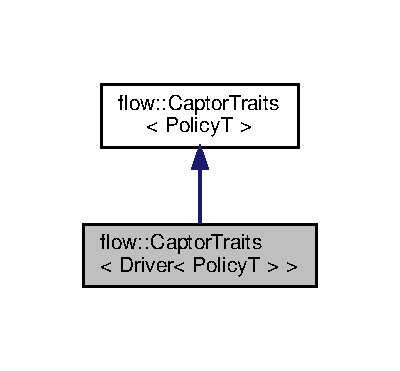
\includegraphics[width=192pt]{structflow_1_1_captor_traits_3_01_driver_3_01_policy_t_01_4_01_4__inherit__graph}
\end{center}
\end{figure}


Collaboration diagram for flow\+:\+:Captor\+Traits$<$ Driver$<$ PolicyT $>$ $>$\+:\nopagebreak
\begin{figure}[H]
\begin{center}
\leavevmode
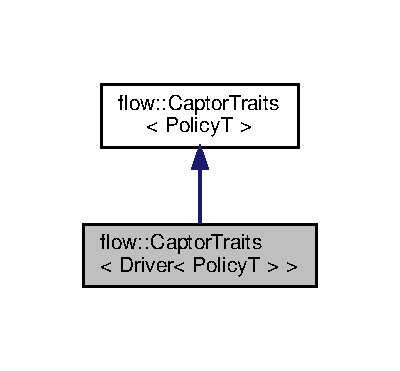
\includegraphics[width=192pt]{structflow_1_1_captor_traits_3_01_driver_3_01_policy_t_01_4_01_4__coll__graph}
\end{center}
\end{figure}


\subsection{Detailed Description}
\subsubsection*{template$<$typename PolicyT$>$\newline
struct flow\+::\+Captor\+Traits$<$ Driver$<$ Policy\+T $>$ $>$}

Traits struct for captor types. 

Requires\+:
\begin{DoxyItemize}
\item {\ttfamily Dispatch\+Type} \+: data dispatch object type
\item {\ttfamily Dispatch\+Container\+Type} \+: container for {\ttfamily Dispatch\+Type} {\ttfamily Dispatch\+Queue\+Monitor\+Type} \+: optional monitoring/capture preconditioning object type
\item {\ttfamily value\+\_\+type} \+: data value type
\item {\ttfamily stamp\+\_\+type} \+: sequence stamp type
\item {\ttfamily size\+\_\+type} \+: integer sizing type
\end{DoxyItemize}


\begin{DoxyTemplParams}{Template Parameters}
{\em CaptorT} & captor type with C\+R\+TP base {\ttfamily \hyperlink{classflow_1_1_captor}{Captor}} \\
\hline
{\em PolicyT} & C\+R\+T\+P-\/derived captor with specialized capture policy \\
\hline
\end{DoxyTemplParams}


The documentation for this struct was generated from the following file\+:\begin{DoxyCompactItemize}
\item 
flow/include/driver/\hyperlink{driver_8h}{driver.\+h}\end{DoxyCompactItemize}

\hypertarget{structflow_1_1_captor_traits_3_01follower_1_1_any_before_3_01_dispatch_t_00_01_lock_policy_t_00_55050b2eb17fc5bc754f0ec7f3a869fd}{}\section{flow\+:\+:Captor\+Traits$<$ follower\+:\+:Any\+Before$<$ DispatchT, Lock\+PolicyT, ContainerT, Queue\+MonitorT $>$ $>$ Struct Template Reference}
\label{structflow_1_1_captor_traits_3_01follower_1_1_any_before_3_01_dispatch_t_00_01_lock_policy_t_00_55050b2eb17fc5bc754f0ec7f3a869fd}\index{flow\+::\+Captor\+Traits$<$ follower\+::\+Any\+Before$<$ Dispatch\+T, Lock\+Policy\+T, Container\+T, Queue\+Monitor\+T $>$ $>$@{flow\+::\+Captor\+Traits$<$ follower\+::\+Any\+Before$<$ Dispatch\+T, Lock\+Policy\+T, Container\+T, Queue\+Monitor\+T $>$ $>$}}


Traits struct for captor types.  




{\ttfamily \#include $<$any\+\_\+before.\+h$>$}



Inheritance diagram for flow\+:\+:Captor\+Traits$<$ follower\+:\+:Any\+Before$<$ DispatchT, Lock\+PolicyT, ContainerT, Queue\+MonitorT $>$ $>$\+:
\nopagebreak
\begin{figure}[H]
\begin{center}
\leavevmode
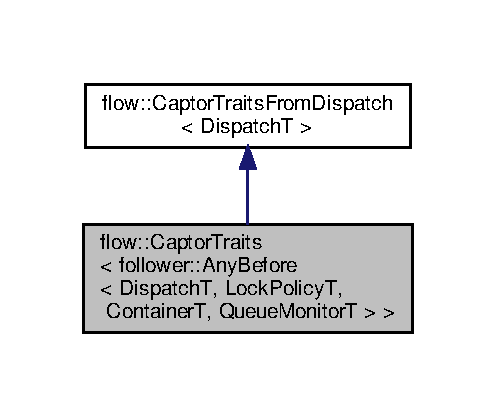
\includegraphics[width=238pt]{structflow_1_1_captor_traits_3_01follower_1_1_any_before_3_01_dispatch_t_00_01_lock_policy_t_00_67d78ed751c12dd4271a62e51f7847c5}
\end{center}
\end{figure}


Collaboration diagram for flow\+:\+:Captor\+Traits$<$ follower\+:\+:Any\+Before$<$ DispatchT, Lock\+PolicyT, ContainerT, Queue\+MonitorT $>$ $>$\+:
\nopagebreak
\begin{figure}[H]
\begin{center}
\leavevmode
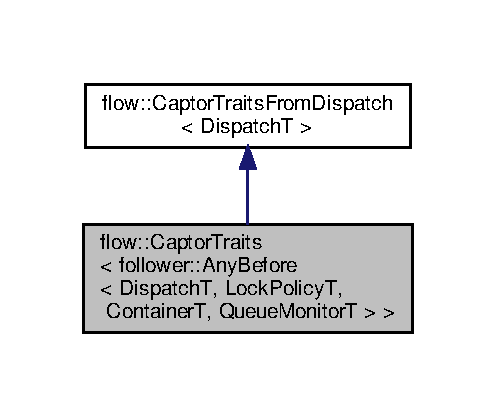
\includegraphics[width=238pt]{structflow_1_1_captor_traits_3_01follower_1_1_any_before_3_01_dispatch_t_00_01_lock_policy_t_00_c5983590e4e1ce28049543603e568672}
\end{center}
\end{figure}
\subsection*{Public Types}
\begin{DoxyCompactItemize}
\item 
\mbox{\Hypertarget{structflow_1_1_captor_traits_3_01follower_1_1_any_before_3_01_dispatch_t_00_01_lock_policy_t_00_55050b2eb17fc5bc754f0ec7f3a869fd_a6a088d321cb4c09f211f0b3fc60e02bd}\label{structflow_1_1_captor_traits_3_01follower_1_1_any_before_3_01_dispatch_t_00_01_lock_policy_t_00_55050b2eb17fc5bc754f0ec7f3a869fd_a6a088d321cb4c09f211f0b3fc60e02bd}} 
using \hyperlink{structflow_1_1_captor_traits_3_01follower_1_1_any_before_3_01_dispatch_t_00_01_lock_policy_t_00_55050b2eb17fc5bc754f0ec7f3a869fd_a6a088d321cb4c09f211f0b3fc60e02bd}{Dispatch\+Container\+Type} = ContainerT
\begin{DoxyCompactList}\small\item\em Underlying dispatch container type. \end{DoxyCompactList}\item 
\mbox{\Hypertarget{structflow_1_1_captor_traits_3_01follower_1_1_any_before_3_01_dispatch_t_00_01_lock_policy_t_00_55050b2eb17fc5bc754f0ec7f3a869fd_a7b78ff288f4063bda4b118d78b92a9a1}\label{structflow_1_1_captor_traits_3_01follower_1_1_any_before_3_01_dispatch_t_00_01_lock_policy_t_00_55050b2eb17fc5bc754f0ec7f3a869fd_a7b78ff288f4063bda4b118d78b92a9a1}} 
using \hyperlink{structflow_1_1_captor_traits_3_01follower_1_1_any_before_3_01_dispatch_t_00_01_lock_policy_t_00_55050b2eb17fc5bc754f0ec7f3a869fd_a7b78ff288f4063bda4b118d78b92a9a1}{Dispatch\+Queue\+Monitor\+Type} = Queue\+MonitorT
\begin{DoxyCompactList}\small\item\em Queue monitor/capture preconditioning type. \end{DoxyCompactList}\item 
\mbox{\Hypertarget{structflow_1_1_captor_traits_3_01follower_1_1_any_before_3_01_dispatch_t_00_01_lock_policy_t_00_55050b2eb17fc5bc754f0ec7f3a869fd_a733e8e2a4231a52cd02c85190713a2ff}\label{structflow_1_1_captor_traits_3_01follower_1_1_any_before_3_01_dispatch_t_00_01_lock_policy_t_00_55050b2eb17fc5bc754f0ec7f3a869fd_a733e8e2a4231a52cd02c85190713a2ff}} 
using \hyperlink{structflow_1_1_captor_traits_3_01follower_1_1_any_before_3_01_dispatch_t_00_01_lock_policy_t_00_55050b2eb17fc5bc754f0ec7f3a869fd_a733e8e2a4231a52cd02c85190713a2ff}{Lock\+Policy\+Type} = Lock\+PolicyT
\begin{DoxyCompactList}\small\item\em Thread locking policy type. \end{DoxyCompactList}\end{DoxyCompactItemize}
\subsection*{Static Public Attributes}
\begin{DoxyCompactItemize}
\item 
static constexpr bool \hyperlink{structflow_1_1_captor_traits_3_01follower_1_1_any_before_3_01_dispatch_t_00_01_lock_policy_t_00_55050b2eb17fc5bc754f0ec7f3a869fd_ae94a381cf76ac9f1a639c58570aa6350}{is\+\_\+capture\+\_\+deterministic} = false
\end{DoxyCompactItemize}


\subsection{Detailed Description}
\subsubsection*{template$<$typename DispatchT, typename Lock\+PolicyT, typename ContainerT, typename Queue\+MonitorT$>$\newline
struct flow\+::\+Captor\+Traits$<$ follower\+::\+Any\+Before$<$ Dispatch\+T, Lock\+Policy\+T, Container\+T, Queue\+Monitor\+T $>$ $>$}

Traits struct for captor types. 

Requires\+:
\begin{DoxyItemize}
\item {\ttfamily Dispatch\+Type} \+: data dispatch object type
\item {\ttfamily Dispatch\+Container\+Type} \+: container for {\ttfamily Dispatch\+Type} {\ttfamily Dispatch\+Queue\+Monitor\+Type} \+: optional monitoring/capture preconditioning object type
\item {\ttfamily value\+\_\+type} \+: data value type
\item {\ttfamily stamp\+\_\+type} \+: sequence stamp type
\item {\ttfamily size\+\_\+type} \+: integer sizing type
\end{DoxyItemize}


\begin{DoxyTemplParams}{Template Parameters}
{\em CaptorT} & captor type with C\+R\+TP base {\ttfamily \hyperlink{classflow_1_1_captor}{Captor}}\\
\hline
{\em DispatchT} & data dispatch type \\
\hline
{\em Lock\+PolicyT} & a Basic\+Lockable (\href{https://en.cppreference.com/w/cpp/named_req/BasicLockable}{\tt https\+://en.\+cppreference.\+com/w/cpp/named\+\_\+req/\+Basic\+Lockable}) object or \hyperlink{structflow_1_1_no_lock}{No\+Lock} or \hyperlink{structflow_1_1_polling_lock}{Polling\+Lock} \\
\hline
{\em ContainerT} & underlying {\ttfamily DispatchT} container type \\
\hline
{\em Queue\+MonitorT} & queue monitor/capture preconditioning type \\
\hline
\end{DoxyTemplParams}


\subsection{Member Data Documentation}
\mbox{\Hypertarget{structflow_1_1_captor_traits_3_01follower_1_1_any_before_3_01_dispatch_t_00_01_lock_policy_t_00_55050b2eb17fc5bc754f0ec7f3a869fd_ae94a381cf76ac9f1a639c58570aa6350}\label{structflow_1_1_captor_traits_3_01follower_1_1_any_before_3_01_dispatch_t_00_01_lock_policy_t_00_55050b2eb17fc5bc754f0ec7f3a869fd_ae94a381cf76ac9f1a639c58570aa6350}} 
\index{flow\+::\+Captor\+Traits$<$ follower\+::\+Any\+Before$<$ Dispatch\+T, Lock\+Policy\+T, Container\+T, Queue\+Monitor\+T $>$ $>$@{flow\+::\+Captor\+Traits$<$ follower\+::\+Any\+Before$<$ Dispatch\+T, Lock\+Policy\+T, Container\+T, Queue\+Monitor\+T $>$ $>$}!is\+\_\+capture\+\_\+deterministic@{is\+\_\+capture\+\_\+deterministic}}
\index{is\+\_\+capture\+\_\+deterministic@{is\+\_\+capture\+\_\+deterministic}!flow\+::\+Captor\+Traits$<$ follower\+::\+Any\+Before$<$ Dispatch\+T, Lock\+Policy\+T, Container\+T, Queue\+Monitor\+T $>$ $>$@{flow\+::\+Captor\+Traits$<$ follower\+::\+Any\+Before$<$ Dispatch\+T, Lock\+Policy\+T, Container\+T, Queue\+Monitor\+T $>$ $>$}}
\subsubsection{\texorpdfstring{is\+\_\+capture\+\_\+deterministic}{is\_capture\_deterministic}}
{\footnotesize\ttfamily template$<$typename DispatchT , typename Lock\+PolicyT , typename ContainerT , typename Queue\+MonitorT $>$ \\
constexpr bool \hyperlink{structflow_1_1_captor_traits}{flow\+::\+Captor\+Traits}$<$ \hyperlink{classflow_1_1follower_1_1_any_before}{follower\+::\+Any\+Before}$<$ DispatchT, Lock\+PolicyT, ContainerT, Queue\+MonitorT $>$ $>$\+::is\+\_\+capture\+\_\+deterministic = false\hspace{0.3cm}{\ttfamily [static]}}

Indicates that data from this captor will N\+OT always be captured deterministically; i.\+e. is always dependent on when data is injected, and when captrue is executed 

The documentation for this struct was generated from the following file\+:\begin{DoxyCompactItemize}
\item 
flow/include/follower/any\+\_\+before.\+h\end{DoxyCompactItemize}

\hypertarget{structflow_1_1_captor_traits_3_01follower_1_1_before_3_01_dispatch_t_00_01_lock_policy_t_00_01_c62c65191d3908e10afd70708af893571}{}\section{flow\+:\+:Captor\+Traits$<$ follower\+:\+:Before$<$ DispatchT, Lock\+PolicyT, ContainerT, Queue\+MonitorT $>$ $>$ Struct Template Reference}
\label{structflow_1_1_captor_traits_3_01follower_1_1_before_3_01_dispatch_t_00_01_lock_policy_t_00_01_c62c65191d3908e10afd70708af893571}\index{flow\+::\+Captor\+Traits$<$ follower\+::\+Before$<$ Dispatch\+T, Lock\+Policy\+T, Container\+T, Queue\+Monitor\+T $>$ $>$@{flow\+::\+Captor\+Traits$<$ follower\+::\+Before$<$ Dispatch\+T, Lock\+Policy\+T, Container\+T, Queue\+Monitor\+T $>$ $>$}}


Traits struct for captor types.  




{\ttfamily \#include $<$before.\+h$>$}



Inheritance diagram for flow\+:\+:Captor\+Traits$<$ follower\+:\+:Before$<$ DispatchT, Lock\+PolicyT, ContainerT, Queue\+MonitorT $>$ $>$\+:
\nopagebreak
\begin{figure}[H]
\begin{center}
\leavevmode
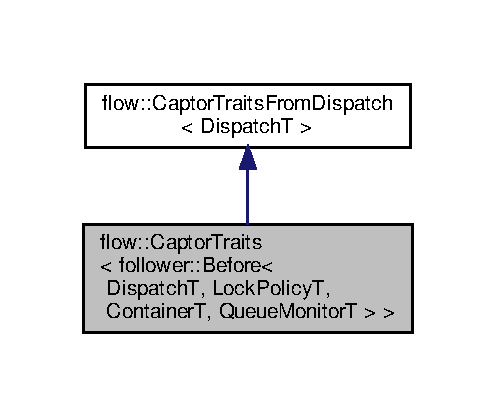
\includegraphics[width=238pt]{structflow_1_1_captor_traits_3_01follower_1_1_before_3_01_dispatch_t_00_01_lock_policy_t_00_01_c88d620e0eba9fa591fae29acc81fecf6}
\end{center}
\end{figure}


Collaboration diagram for flow\+:\+:Captor\+Traits$<$ follower\+:\+:Before$<$ DispatchT, Lock\+PolicyT, ContainerT, Queue\+MonitorT $>$ $>$\+:
\nopagebreak
\begin{figure}[H]
\begin{center}
\leavevmode
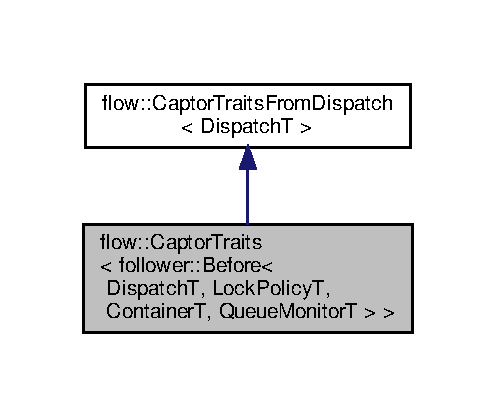
\includegraphics[width=238pt]{structflow_1_1_captor_traits_3_01follower_1_1_before_3_01_dispatch_t_00_01_lock_policy_t_00_01_c297c7fc392fcee21430e63ee294690bb}
\end{center}
\end{figure}
\subsection*{Public Types}
\begin{DoxyCompactItemize}
\item 
\mbox{\Hypertarget{structflow_1_1_captor_traits_3_01follower_1_1_before_3_01_dispatch_t_00_01_lock_policy_t_00_01_c62c65191d3908e10afd70708af893571_a3fdfb8ee153c76576b8d28881ff88671}\label{structflow_1_1_captor_traits_3_01follower_1_1_before_3_01_dispatch_t_00_01_lock_policy_t_00_01_c62c65191d3908e10afd70708af893571_a3fdfb8ee153c76576b8d28881ff88671}} 
using \hyperlink{structflow_1_1_captor_traits_3_01follower_1_1_before_3_01_dispatch_t_00_01_lock_policy_t_00_01_c62c65191d3908e10afd70708af893571_a3fdfb8ee153c76576b8d28881ff88671}{Dispatch\+Container\+Type} = ContainerT
\begin{DoxyCompactList}\small\item\em Underlying dispatch container type. \end{DoxyCompactList}\item 
\mbox{\Hypertarget{structflow_1_1_captor_traits_3_01follower_1_1_before_3_01_dispatch_t_00_01_lock_policy_t_00_01_c62c65191d3908e10afd70708af893571_a0cebb7ccb35160a01a447be8cac2357f}\label{structflow_1_1_captor_traits_3_01follower_1_1_before_3_01_dispatch_t_00_01_lock_policy_t_00_01_c62c65191d3908e10afd70708af893571_a0cebb7ccb35160a01a447be8cac2357f}} 
using \hyperlink{structflow_1_1_captor_traits_3_01follower_1_1_before_3_01_dispatch_t_00_01_lock_policy_t_00_01_c62c65191d3908e10afd70708af893571_a0cebb7ccb35160a01a447be8cac2357f}{Dispatch\+Queue\+Monitor\+Type} = Queue\+MonitorT
\begin{DoxyCompactList}\small\item\em Queue monitor/capture preconditioning type. \end{DoxyCompactList}\item 
\mbox{\Hypertarget{structflow_1_1_captor_traits_3_01follower_1_1_before_3_01_dispatch_t_00_01_lock_policy_t_00_01_c62c65191d3908e10afd70708af893571_a39edb10c59799215b617992b09f5cfec}\label{structflow_1_1_captor_traits_3_01follower_1_1_before_3_01_dispatch_t_00_01_lock_policy_t_00_01_c62c65191d3908e10afd70708af893571_a39edb10c59799215b617992b09f5cfec}} 
using \hyperlink{structflow_1_1_captor_traits_3_01follower_1_1_before_3_01_dispatch_t_00_01_lock_policy_t_00_01_c62c65191d3908e10afd70708af893571_a39edb10c59799215b617992b09f5cfec}{Lock\+Policy\+Type} = Lock\+PolicyT
\begin{DoxyCompactList}\small\item\em Thread locking policy type. \end{DoxyCompactList}\end{DoxyCompactItemize}
\subsection*{Static Public Attributes}
\begin{DoxyCompactItemize}
\item 
static constexpr bool \hyperlink{structflow_1_1_captor_traits_3_01follower_1_1_before_3_01_dispatch_t_00_01_lock_policy_t_00_01_c62c65191d3908e10afd70708af893571_a84e9d853507aea739c13eef4367500cc}{is\+\_\+capture\+\_\+deterministic} = true
\end{DoxyCompactItemize}


\subsection{Detailed Description}
\subsubsection*{template$<$typename DispatchT, typename Lock\+PolicyT, typename ContainerT, typename Queue\+MonitorT$>$\newline
struct flow\+::\+Captor\+Traits$<$ follower\+::\+Before$<$ Dispatch\+T, Lock\+Policy\+T, Container\+T, Queue\+Monitor\+T $>$ $>$}

Traits struct for captor types. 

Requires\+:
\begin{DoxyItemize}
\item {\ttfamily Dispatch\+Type} \+: data dispatch object type
\item {\ttfamily Dispatch\+Container\+Type} \+: container for {\ttfamily Dispatch\+Type} {\ttfamily Dispatch\+Queue\+Monitor\+Type} \+: optional monitoring/capture preconditioning object type
\item {\ttfamily value\+\_\+type} \+: data value type
\item {\ttfamily stamp\+\_\+type} \+: sequence stamp type
\item {\ttfamily size\+\_\+type} \+: integer sizing type
\end{DoxyItemize}


\begin{DoxyTemplParams}{Template Parameters}
{\em CaptorT} & captor type with C\+R\+TP base {\ttfamily \hyperlink{classflow_1_1_captor}{Captor}}\\
\hline
{\em DispatchT} & data dispatch type \\
\hline
{\em Lock\+PolicyT} & a Basic\+Lockable (\href{https://en.cppreference.com/w/cpp/named_req/BasicLockable}{\tt https\+://en.\+cppreference.\+com/w/cpp/named\+\_\+req/\+Basic\+Lockable}) object or \hyperlink{structflow_1_1_no_lock}{No\+Lock} or \hyperlink{structflow_1_1_polling_lock}{Polling\+Lock} \\
\hline
{\em ContainerT} & underlying {\ttfamily DispatchT} container type \\
\hline
{\em Queue\+MonitorT} & queue monitor/capture preconditioning type \\
\hline
\end{DoxyTemplParams}


\subsection{Member Data Documentation}
\mbox{\Hypertarget{structflow_1_1_captor_traits_3_01follower_1_1_before_3_01_dispatch_t_00_01_lock_policy_t_00_01_c62c65191d3908e10afd70708af893571_a84e9d853507aea739c13eef4367500cc}\label{structflow_1_1_captor_traits_3_01follower_1_1_before_3_01_dispatch_t_00_01_lock_policy_t_00_01_c62c65191d3908e10afd70708af893571_a84e9d853507aea739c13eef4367500cc}} 
\index{flow\+::\+Captor\+Traits$<$ follower\+::\+Before$<$ Dispatch\+T, Lock\+Policy\+T, Container\+T, Queue\+Monitor\+T $>$ $>$@{flow\+::\+Captor\+Traits$<$ follower\+::\+Before$<$ Dispatch\+T, Lock\+Policy\+T, Container\+T, Queue\+Monitor\+T $>$ $>$}!is\+\_\+capture\+\_\+deterministic@{is\+\_\+capture\+\_\+deterministic}}
\index{is\+\_\+capture\+\_\+deterministic@{is\+\_\+capture\+\_\+deterministic}!flow\+::\+Captor\+Traits$<$ follower\+::\+Before$<$ Dispatch\+T, Lock\+Policy\+T, Container\+T, Queue\+Monitor\+T $>$ $>$@{flow\+::\+Captor\+Traits$<$ follower\+::\+Before$<$ Dispatch\+T, Lock\+Policy\+T, Container\+T, Queue\+Monitor\+T $>$ $>$}}
\subsubsection{\texorpdfstring{is\+\_\+capture\+\_\+deterministic}{is\_capture\_deterministic}}
{\footnotesize\ttfamily template$<$typename DispatchT , typename Lock\+PolicyT , typename ContainerT , typename Queue\+MonitorT $>$ \\
constexpr bool \hyperlink{structflow_1_1_captor_traits}{flow\+::\+Captor\+Traits}$<$ \hyperlink{classflow_1_1follower_1_1_before}{follower\+::\+Before}$<$ DispatchT, Lock\+PolicyT, ContainerT, Queue\+MonitorT $>$ $>$\+::is\+\_\+capture\+\_\+deterministic = true\hspace{0.3cm}{\ttfamily [static]}}

Indicates that data from this captor will always be captured deterministically, so long as data injection is monotonically sequenced 

The documentation for this struct was generated from the following file\+:\begin{DoxyCompactItemize}
\item 
flow/include/follower/\hyperlink{before_8h}{before.\+h}\end{DoxyCompactItemize}

\hypertarget{structflow_1_1_captor_traits_3_01follower_1_1_closest_before_3_01_dispatch_t_00_01_lock_policy_t8b834bc2517b16c76af22e1a13353500}{}\section{flow\+:\+:Captor\+Traits$<$ follower\+:\+:Closest\+Before$<$ DispatchT, Lock\+PolicyT, ContainerT, Queue\+MonitorT $>$ $>$ Struct Template Reference}
\label{structflow_1_1_captor_traits_3_01follower_1_1_closest_before_3_01_dispatch_t_00_01_lock_policy_t8b834bc2517b16c76af22e1a13353500}\index{flow\+::\+Captor\+Traits$<$ follower\+::\+Closest\+Before$<$ Dispatch\+T, Lock\+Policy\+T, Container\+T, Queue\+Monitor\+T $>$ $>$@{flow\+::\+Captor\+Traits$<$ follower\+::\+Closest\+Before$<$ Dispatch\+T, Lock\+Policy\+T, Container\+T, Queue\+Monitor\+T $>$ $>$}}


Traits struct for captor types.  




{\ttfamily \#include $<$closest\+\_\+before.\+h$>$}



Inheritance diagram for flow\+:\+:Captor\+Traits$<$ follower\+:\+:Closest\+Before$<$ DispatchT, Lock\+PolicyT, ContainerT, Queue\+MonitorT $>$ $>$\+:
\nopagebreak
\begin{figure}[H]
\begin{center}
\leavevmode
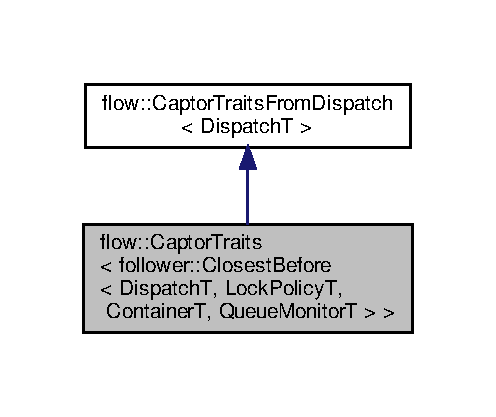
\includegraphics[width=238pt]{structflow_1_1_captor_traits_3_01follower_1_1_closest_before_3_01_dispatch_t_00_01_lock_policy_td890bbd5f0d590aef7cd8d5b40ba8ec5}
\end{center}
\end{figure}


Collaboration diagram for flow\+:\+:Captor\+Traits$<$ follower\+:\+:Closest\+Before$<$ DispatchT, Lock\+PolicyT, ContainerT, Queue\+MonitorT $>$ $>$\+:
\nopagebreak
\begin{figure}[H]
\begin{center}
\leavevmode
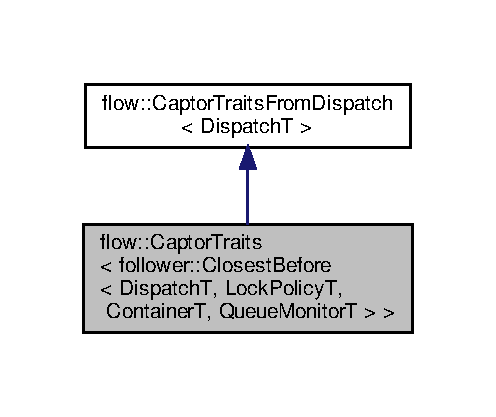
\includegraphics[width=238pt]{structflow_1_1_captor_traits_3_01follower_1_1_closest_before_3_01_dispatch_t_00_01_lock_policy_te2d2da6c11e1cd723d360f7d301ea924}
\end{center}
\end{figure}
\subsection*{Public Types}
\begin{DoxyCompactItemize}
\item 
\mbox{\Hypertarget{structflow_1_1_captor_traits_3_01follower_1_1_closest_before_3_01_dispatch_t_00_01_lock_policy_t8b834bc2517b16c76af22e1a13353500_a45e8c31040b732922ebdb421a6bfc2df}\label{structflow_1_1_captor_traits_3_01follower_1_1_closest_before_3_01_dispatch_t_00_01_lock_policy_t8b834bc2517b16c76af22e1a13353500_a45e8c31040b732922ebdb421a6bfc2df}} 
using \hyperlink{structflow_1_1_captor_traits_3_01follower_1_1_closest_before_3_01_dispatch_t_00_01_lock_policy_t8b834bc2517b16c76af22e1a13353500_a45e8c31040b732922ebdb421a6bfc2df}{Dispatch\+Container\+Type} = ContainerT
\begin{DoxyCompactList}\small\item\em Underlying dispatch container type. \end{DoxyCompactList}\item 
\mbox{\Hypertarget{structflow_1_1_captor_traits_3_01follower_1_1_closest_before_3_01_dispatch_t_00_01_lock_policy_t8b834bc2517b16c76af22e1a13353500_aa182722483ded4d60cbc2f386d9c6353}\label{structflow_1_1_captor_traits_3_01follower_1_1_closest_before_3_01_dispatch_t_00_01_lock_policy_t8b834bc2517b16c76af22e1a13353500_aa182722483ded4d60cbc2f386d9c6353}} 
using \hyperlink{structflow_1_1_captor_traits_3_01follower_1_1_closest_before_3_01_dispatch_t_00_01_lock_policy_t8b834bc2517b16c76af22e1a13353500_aa182722483ded4d60cbc2f386d9c6353}{Dispatch\+Queue\+Monitor\+Type} = Queue\+MonitorT
\begin{DoxyCompactList}\small\item\em Queue monitor/capture preconditioning type. \end{DoxyCompactList}\item 
\mbox{\Hypertarget{structflow_1_1_captor_traits_3_01follower_1_1_closest_before_3_01_dispatch_t_00_01_lock_policy_t8b834bc2517b16c76af22e1a13353500_ad1a3d53bf296ab75c137e81925eefe78}\label{structflow_1_1_captor_traits_3_01follower_1_1_closest_before_3_01_dispatch_t_00_01_lock_policy_t8b834bc2517b16c76af22e1a13353500_ad1a3d53bf296ab75c137e81925eefe78}} 
using \hyperlink{structflow_1_1_captor_traits_3_01follower_1_1_closest_before_3_01_dispatch_t_00_01_lock_policy_t8b834bc2517b16c76af22e1a13353500_ad1a3d53bf296ab75c137e81925eefe78}{Lock\+Policy\+Type} = Lock\+PolicyT
\begin{DoxyCompactList}\small\item\em Thread locking policy type. \end{DoxyCompactList}\end{DoxyCompactItemize}
\subsection*{Static Public Attributes}
\begin{DoxyCompactItemize}
\item 
static constexpr bool \hyperlink{structflow_1_1_captor_traits_3_01follower_1_1_closest_before_3_01_dispatch_t_00_01_lock_policy_t8b834bc2517b16c76af22e1a13353500_a30e638a2c1b9a6c02d59b0817a29ef62}{is\+\_\+capture\+\_\+deterministic} = true
\end{DoxyCompactItemize}


\subsection{Detailed Description}
\subsubsection*{template$<$typename DispatchT, typename Lock\+PolicyT, typename ContainerT, typename Queue\+MonitorT$>$\newline
struct flow\+::\+Captor\+Traits$<$ follower\+::\+Closest\+Before$<$ Dispatch\+T, Lock\+Policy\+T, Container\+T, Queue\+Monitor\+T $>$ $>$}

Traits struct for captor types. 

Requires\+:
\begin{DoxyItemize}
\item {\ttfamily Dispatch\+Type} \+: data dispatch object type
\item {\ttfamily Dispatch\+Container\+Type} \+: container for {\ttfamily Dispatch\+Type} {\ttfamily Dispatch\+Queue\+Monitor\+Type} \+: optional monitoring/capture preconditioning object type
\item {\ttfamily value\+\_\+type} \+: data value type
\item {\ttfamily stamp\+\_\+type} \+: sequence stamp type
\item {\ttfamily size\+\_\+type} \+: integer sizing type
\end{DoxyItemize}


\begin{DoxyTemplParams}{Template Parameters}
{\em CaptorT} & captor type with C\+R\+TP base {\ttfamily \hyperlink{classflow_1_1_captor}{Captor}}\\
\hline
{\em DispatchT} & data dispatch type \\
\hline
{\em Lock\+PolicyT} & a Basic\+Lockable (\href{https://en.cppreference.com/w/cpp/named_req/BasicLockable}{\tt https\+://en.\+cppreference.\+com/w/cpp/named\+\_\+req/\+Basic\+Lockable}) object or \hyperlink{structflow_1_1_no_lock}{No\+Lock} or \hyperlink{structflow_1_1_polling_lock}{Polling\+Lock} \\
\hline
{\em ContainerT} & underlying {\ttfamily DispatchT} container type \\
\hline
{\em Queue\+MonitorT} & queue monitor/capture preconditioning type \\
\hline
\end{DoxyTemplParams}


\subsection{Member Data Documentation}
\mbox{\Hypertarget{structflow_1_1_captor_traits_3_01follower_1_1_closest_before_3_01_dispatch_t_00_01_lock_policy_t8b834bc2517b16c76af22e1a13353500_a30e638a2c1b9a6c02d59b0817a29ef62}\label{structflow_1_1_captor_traits_3_01follower_1_1_closest_before_3_01_dispatch_t_00_01_lock_policy_t8b834bc2517b16c76af22e1a13353500_a30e638a2c1b9a6c02d59b0817a29ef62}} 
\index{flow\+::\+Captor\+Traits$<$ follower\+::\+Closest\+Before$<$ Dispatch\+T, Lock\+Policy\+T, Container\+T, Queue\+Monitor\+T $>$ $>$@{flow\+::\+Captor\+Traits$<$ follower\+::\+Closest\+Before$<$ Dispatch\+T, Lock\+Policy\+T, Container\+T, Queue\+Monitor\+T $>$ $>$}!is\+\_\+capture\+\_\+deterministic@{is\+\_\+capture\+\_\+deterministic}}
\index{is\+\_\+capture\+\_\+deterministic@{is\+\_\+capture\+\_\+deterministic}!flow\+::\+Captor\+Traits$<$ follower\+::\+Closest\+Before$<$ Dispatch\+T, Lock\+Policy\+T, Container\+T, Queue\+Monitor\+T $>$ $>$@{flow\+::\+Captor\+Traits$<$ follower\+::\+Closest\+Before$<$ Dispatch\+T, Lock\+Policy\+T, Container\+T, Queue\+Monitor\+T $>$ $>$}}
\subsubsection{\texorpdfstring{is\+\_\+capture\+\_\+deterministic}{is\_capture\_deterministic}}
{\footnotesize\ttfamily template$<$typename DispatchT , typename Lock\+PolicyT , typename ContainerT , typename Queue\+MonitorT $>$ \\
constexpr bool \hyperlink{structflow_1_1_captor_traits}{flow\+::\+Captor\+Traits}$<$ \hyperlink{classflow_1_1follower_1_1_closest_before}{follower\+::\+Closest\+Before}$<$ DispatchT, Lock\+PolicyT, ContainerT, Queue\+MonitorT $>$ $>$\+::is\+\_\+capture\+\_\+deterministic = true\hspace{0.3cm}{\ttfamily [static]}}

Indicates that data from this captor will always be captured deterministically, so long as data injection is monotonically sequenced 

The documentation for this struct was generated from the following file\+:\begin{DoxyCompactItemize}
\item 
flow/include/follower/\hyperlink{closest__before_8h}{closest\+\_\+before.\+h}\end{DoxyCompactItemize}

\hypertarget{structflow_1_1_captor_traits_3_01follower_1_1_count_before_3_01_dispatch_t_00_01_lock_policy_t_0d08c28482191f4a9fdac77c50d53921d}{}\section{flow\+:\+:Captor\+Traits$<$ follower\+:\+:Count\+Before$<$ DispatchT, Lock\+PolicyT, ContainerT, Queue\+MonitorT $>$ $>$ Struct Template Reference}
\label{structflow_1_1_captor_traits_3_01follower_1_1_count_before_3_01_dispatch_t_00_01_lock_policy_t_0d08c28482191f4a9fdac77c50d53921d}\index{flow\+::\+Captor\+Traits$<$ follower\+::\+Count\+Before$<$ Dispatch\+T, Lock\+Policy\+T, Container\+T, Queue\+Monitor\+T $>$ $>$@{flow\+::\+Captor\+Traits$<$ follower\+::\+Count\+Before$<$ Dispatch\+T, Lock\+Policy\+T, Container\+T, Queue\+Monitor\+T $>$ $>$}}


Traits struct for captor types.  




{\ttfamily \#include $<$count\+\_\+before.\+h$>$}



Inheritance diagram for flow\+:\+:Captor\+Traits$<$ follower\+:\+:Count\+Before$<$ DispatchT, Lock\+PolicyT, ContainerT, Queue\+MonitorT $>$ $>$\+:
\nopagebreak
\begin{figure}[H]
\begin{center}
\leavevmode
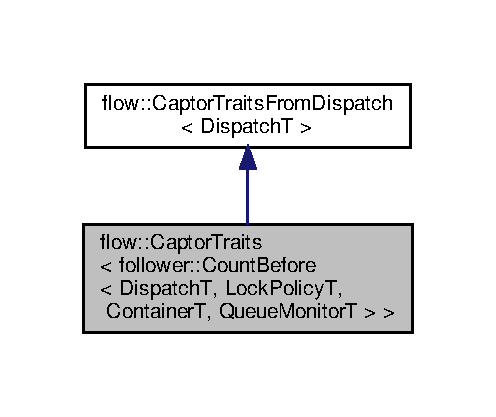
\includegraphics[width=238pt]{structflow_1_1_captor_traits_3_01follower_1_1_count_before_3_01_dispatch_t_00_01_lock_policy_t_04f3cbc9817388fcf78dbf71649207fe7}
\end{center}
\end{figure}


Collaboration diagram for flow\+:\+:Captor\+Traits$<$ follower\+:\+:Count\+Before$<$ DispatchT, Lock\+PolicyT, ContainerT, Queue\+MonitorT $>$ $>$\+:
\nopagebreak
\begin{figure}[H]
\begin{center}
\leavevmode
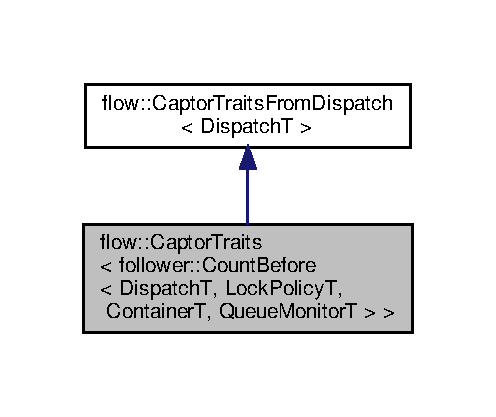
\includegraphics[width=238pt]{structflow_1_1_captor_traits_3_01follower_1_1_count_before_3_01_dispatch_t_00_01_lock_policy_t_0820a9c27addcee2bc74a2035c4799b6d}
\end{center}
\end{figure}
\subsection*{Public Types}
\begin{DoxyCompactItemize}
\item 
\mbox{\Hypertarget{structflow_1_1_captor_traits_3_01follower_1_1_count_before_3_01_dispatch_t_00_01_lock_policy_t_0d08c28482191f4a9fdac77c50d53921d_a910c2579450b9ddea7e2ca447644318a}\label{structflow_1_1_captor_traits_3_01follower_1_1_count_before_3_01_dispatch_t_00_01_lock_policy_t_0d08c28482191f4a9fdac77c50d53921d_a910c2579450b9ddea7e2ca447644318a}} 
using \hyperlink{structflow_1_1_captor_traits_3_01follower_1_1_count_before_3_01_dispatch_t_00_01_lock_policy_t_0d08c28482191f4a9fdac77c50d53921d_a910c2579450b9ddea7e2ca447644318a}{Dispatch\+Container\+Type} = ContainerT
\begin{DoxyCompactList}\small\item\em Underlying dispatch container type. \end{DoxyCompactList}\item 
\mbox{\Hypertarget{structflow_1_1_captor_traits_3_01follower_1_1_count_before_3_01_dispatch_t_00_01_lock_policy_t_0d08c28482191f4a9fdac77c50d53921d_a6169c0a8254301865de88e30d47fd1e8}\label{structflow_1_1_captor_traits_3_01follower_1_1_count_before_3_01_dispatch_t_00_01_lock_policy_t_0d08c28482191f4a9fdac77c50d53921d_a6169c0a8254301865de88e30d47fd1e8}} 
using \hyperlink{structflow_1_1_captor_traits_3_01follower_1_1_count_before_3_01_dispatch_t_00_01_lock_policy_t_0d08c28482191f4a9fdac77c50d53921d_a6169c0a8254301865de88e30d47fd1e8}{Dispatch\+Queue\+Monitor\+Type} = Queue\+MonitorT
\begin{DoxyCompactList}\small\item\em Queue monitor/capture preconditioning type. \end{DoxyCompactList}\item 
\mbox{\Hypertarget{structflow_1_1_captor_traits_3_01follower_1_1_count_before_3_01_dispatch_t_00_01_lock_policy_t_0d08c28482191f4a9fdac77c50d53921d_a62b4fb8b787875e6878a7cb1d5c451e1}\label{structflow_1_1_captor_traits_3_01follower_1_1_count_before_3_01_dispatch_t_00_01_lock_policy_t_0d08c28482191f4a9fdac77c50d53921d_a62b4fb8b787875e6878a7cb1d5c451e1}} 
using \hyperlink{structflow_1_1_captor_traits_3_01follower_1_1_count_before_3_01_dispatch_t_00_01_lock_policy_t_0d08c28482191f4a9fdac77c50d53921d_a62b4fb8b787875e6878a7cb1d5c451e1}{Lock\+Policy\+Type} = Lock\+PolicyT
\begin{DoxyCompactList}\small\item\em Thread locking policy type. \end{DoxyCompactList}\end{DoxyCompactItemize}
\subsection*{Static Public Attributes}
\begin{DoxyCompactItemize}
\item 
static constexpr bool \hyperlink{structflow_1_1_captor_traits_3_01follower_1_1_count_before_3_01_dispatch_t_00_01_lock_policy_t_0d08c28482191f4a9fdac77c50d53921d_a1e7e3deda342f19b5c2df4c3a66f7af8}{is\+\_\+capture\+\_\+deterministic} = false
\end{DoxyCompactItemize}


\subsection{Detailed Description}
\subsubsection*{template$<$typename DispatchT, typename Lock\+PolicyT, typename ContainerT, typename Queue\+MonitorT$>$\newline
struct flow\+::\+Captor\+Traits$<$ follower\+::\+Count\+Before$<$ Dispatch\+T, Lock\+Policy\+T, Container\+T, Queue\+Monitor\+T $>$ $>$}

Traits struct for captor types. 

Requires\+:
\begin{DoxyItemize}
\item {\ttfamily Dispatch\+Type} \+: data dispatch object type
\item {\ttfamily Dispatch\+Container\+Type} \+: container for {\ttfamily Dispatch\+Type} {\ttfamily Dispatch\+Queue\+Monitor\+Type} \+: optional monitoring/capture preconditioning object type
\item {\ttfamily value\+\_\+type} \+: data value type
\item {\ttfamily stamp\+\_\+type} \+: sequence stamp type
\item {\ttfamily size\+\_\+type} \+: integer sizing type
\end{DoxyItemize}


\begin{DoxyTemplParams}{Template Parameters}
{\em CaptorT} & captor type with C\+R\+TP base {\ttfamily \hyperlink{classflow_1_1_captor}{Captor}}\\
\hline
{\em DispatchT} & data dispatch type \\
\hline
{\em Lock\+PolicyT} & a Basic\+Lockable (\href{https://en.cppreference.com/w/cpp/named_req/BasicLockable}{\tt https\+://en.\+cppreference.\+com/w/cpp/named\+\_\+req/\+Basic\+Lockable}) object or \hyperlink{structflow_1_1_no_lock}{No\+Lock} or \hyperlink{structflow_1_1_polling_lock}{Polling\+Lock} \\
\hline
{\em ContainerT} & underlying {\ttfamily DispatchT} container type \\
\hline
{\em Queue\+MonitorT} & queue monitor/capture preconditioning type \\
\hline
\end{DoxyTemplParams}


\subsection{Member Data Documentation}
\mbox{\Hypertarget{structflow_1_1_captor_traits_3_01follower_1_1_count_before_3_01_dispatch_t_00_01_lock_policy_t_0d08c28482191f4a9fdac77c50d53921d_a1e7e3deda342f19b5c2df4c3a66f7af8}\label{structflow_1_1_captor_traits_3_01follower_1_1_count_before_3_01_dispatch_t_00_01_lock_policy_t_0d08c28482191f4a9fdac77c50d53921d_a1e7e3deda342f19b5c2df4c3a66f7af8}} 
\index{flow\+::\+Captor\+Traits$<$ follower\+::\+Count\+Before$<$ Dispatch\+T, Lock\+Policy\+T, Container\+T, Queue\+Monitor\+T $>$ $>$@{flow\+::\+Captor\+Traits$<$ follower\+::\+Count\+Before$<$ Dispatch\+T, Lock\+Policy\+T, Container\+T, Queue\+Monitor\+T $>$ $>$}!is\+\_\+capture\+\_\+deterministic@{is\+\_\+capture\+\_\+deterministic}}
\index{is\+\_\+capture\+\_\+deterministic@{is\+\_\+capture\+\_\+deterministic}!flow\+::\+Captor\+Traits$<$ follower\+::\+Count\+Before$<$ Dispatch\+T, Lock\+Policy\+T, Container\+T, Queue\+Monitor\+T $>$ $>$@{flow\+::\+Captor\+Traits$<$ follower\+::\+Count\+Before$<$ Dispatch\+T, Lock\+Policy\+T, Container\+T, Queue\+Monitor\+T $>$ $>$}}
\subsubsection{\texorpdfstring{is\+\_\+capture\+\_\+deterministic}{is\_capture\_deterministic}}
{\footnotesize\ttfamily template$<$typename DispatchT , typename Lock\+PolicyT , typename ContainerT , typename Queue\+MonitorT $>$ \\
constexpr bool \hyperlink{structflow_1_1_captor_traits}{flow\+::\+Captor\+Traits}$<$ \hyperlink{classflow_1_1follower_1_1_count_before}{follower\+::\+Count\+Before}$<$ DispatchT, Lock\+PolicyT, ContainerT, Queue\+MonitorT $>$ $>$\+::is\+\_\+capture\+\_\+deterministic = false\hspace{0.3cm}{\ttfamily [static]}}

Indicates that data from this captor will N\+OT always be captured deterministically; i.\+e. is always dependent on when data is injected, and when captrue is executed 

The documentation for this struct was generated from the following file\+:\begin{DoxyCompactItemize}
\item 
flow/include/follower/\hyperlink{count__before_8h}{count\+\_\+before.\+h}\end{DoxyCompactItemize}

\hypertarget{structflow_1_1_captor_traits_3_01follower_1_1_latched_3_01_dispatch_t_00_01_lock_policy_t_00_01_7069ffe3c5f41ae454dc415b835f945a}{}\section{flow\+:\+:Captor\+Traits$<$ follower\+:\+:Latched$<$ DispatchT, Lock\+PolicyT, ContainerT, Queue\+MonitorT $>$ $>$ Struct Template Reference}
\label{structflow_1_1_captor_traits_3_01follower_1_1_latched_3_01_dispatch_t_00_01_lock_policy_t_00_01_7069ffe3c5f41ae454dc415b835f945a}\index{flow\+::\+Captor\+Traits$<$ follower\+::\+Latched$<$ Dispatch\+T, Lock\+Policy\+T, Container\+T, Queue\+Monitor\+T $>$ $>$@{flow\+::\+Captor\+Traits$<$ follower\+::\+Latched$<$ Dispatch\+T, Lock\+Policy\+T, Container\+T, Queue\+Monitor\+T $>$ $>$}}


Traits struct for captor types.  




{\ttfamily \#include $<$latched.\+h$>$}



Inheritance diagram for flow\+:\+:Captor\+Traits$<$ follower\+:\+:Latched$<$ DispatchT, Lock\+PolicyT, ContainerT, Queue\+MonitorT $>$ $>$\+:
\nopagebreak
\begin{figure}[H]
\begin{center}
\leavevmode
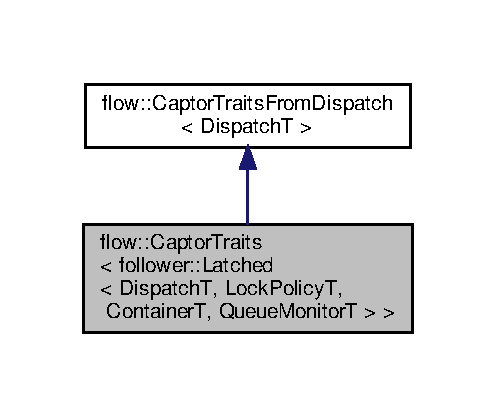
\includegraphics[width=238pt]{structflow_1_1_captor_traits_3_01follower_1_1_latched_3_01_dispatch_t_00_01_lock_policy_t_00_01_3b9e00ddf2349f1533eca02f3abf2d0f}
\end{center}
\end{figure}


Collaboration diagram for flow\+:\+:Captor\+Traits$<$ follower\+:\+:Latched$<$ DispatchT, Lock\+PolicyT, ContainerT, Queue\+MonitorT $>$ $>$\+:
\nopagebreak
\begin{figure}[H]
\begin{center}
\leavevmode
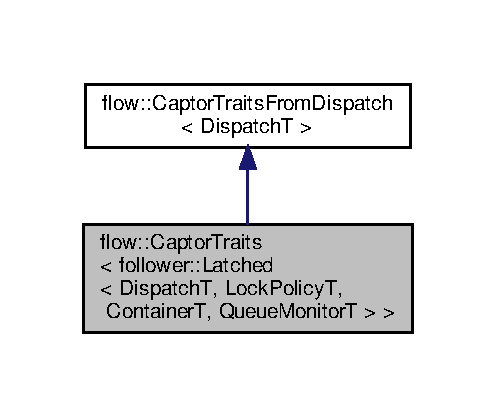
\includegraphics[width=238pt]{structflow_1_1_captor_traits_3_01follower_1_1_latched_3_01_dispatch_t_00_01_lock_policy_t_00_01_0a454d79367eed3f91b8ffa394457121}
\end{center}
\end{figure}
\subsection*{Public Types}
\begin{DoxyCompactItemize}
\item 
\mbox{\Hypertarget{structflow_1_1_captor_traits_3_01follower_1_1_latched_3_01_dispatch_t_00_01_lock_policy_t_00_01_7069ffe3c5f41ae454dc415b835f945a_a59a9451ab6b2976466800c18e6e26ed5}\label{structflow_1_1_captor_traits_3_01follower_1_1_latched_3_01_dispatch_t_00_01_lock_policy_t_00_01_7069ffe3c5f41ae454dc415b835f945a_a59a9451ab6b2976466800c18e6e26ed5}} 
using \hyperlink{structflow_1_1_captor_traits_3_01follower_1_1_latched_3_01_dispatch_t_00_01_lock_policy_t_00_01_7069ffe3c5f41ae454dc415b835f945a_a59a9451ab6b2976466800c18e6e26ed5}{Dispatch\+Container\+Type} = ContainerT
\begin{DoxyCompactList}\small\item\em Underlying dispatch container type. \end{DoxyCompactList}\item 
\mbox{\Hypertarget{structflow_1_1_captor_traits_3_01follower_1_1_latched_3_01_dispatch_t_00_01_lock_policy_t_00_01_7069ffe3c5f41ae454dc415b835f945a_ab8735edae4f4dba8e4c5f9f46a9239ba}\label{structflow_1_1_captor_traits_3_01follower_1_1_latched_3_01_dispatch_t_00_01_lock_policy_t_00_01_7069ffe3c5f41ae454dc415b835f945a_ab8735edae4f4dba8e4c5f9f46a9239ba}} 
using \hyperlink{structflow_1_1_captor_traits_3_01follower_1_1_latched_3_01_dispatch_t_00_01_lock_policy_t_00_01_7069ffe3c5f41ae454dc415b835f945a_ab8735edae4f4dba8e4c5f9f46a9239ba}{Dispatch\+Queue\+Monitor\+Type} = Queue\+MonitorT
\begin{DoxyCompactList}\small\item\em Queue monitor/capture preconditioning type. \end{DoxyCompactList}\item 
\mbox{\Hypertarget{structflow_1_1_captor_traits_3_01follower_1_1_latched_3_01_dispatch_t_00_01_lock_policy_t_00_01_7069ffe3c5f41ae454dc415b835f945a_aa1d0f17c8ee6577875dab5d082d759a2}\label{structflow_1_1_captor_traits_3_01follower_1_1_latched_3_01_dispatch_t_00_01_lock_policy_t_00_01_7069ffe3c5f41ae454dc415b835f945a_aa1d0f17c8ee6577875dab5d082d759a2}} 
using \hyperlink{structflow_1_1_captor_traits_3_01follower_1_1_latched_3_01_dispatch_t_00_01_lock_policy_t_00_01_7069ffe3c5f41ae454dc415b835f945a_aa1d0f17c8ee6577875dab5d082d759a2}{Lock\+Policy\+Type} = Lock\+PolicyT
\begin{DoxyCompactList}\small\item\em Thread locking policy type. \end{DoxyCompactList}\end{DoxyCompactItemize}
\subsection*{Static Public Attributes}
\begin{DoxyCompactItemize}
\item 
static constexpr bool \hyperlink{structflow_1_1_captor_traits_3_01follower_1_1_latched_3_01_dispatch_t_00_01_lock_policy_t_00_01_7069ffe3c5f41ae454dc415b835f945a_a1658ae448bc61a7b26d895c405672e9b}{is\+\_\+capture\+\_\+deterministic} = false
\end{DoxyCompactItemize}


\subsection{Detailed Description}
\subsubsection*{template$<$typename DispatchT, typename Lock\+PolicyT, typename ContainerT, typename Queue\+MonitorT$>$\newline
struct flow\+::\+Captor\+Traits$<$ follower\+::\+Latched$<$ Dispatch\+T, Lock\+Policy\+T, Container\+T, Queue\+Monitor\+T $>$ $>$}

Traits struct for captor types. 

Requires\+:
\begin{DoxyItemize}
\item {\ttfamily Dispatch\+Type} \+: data dispatch object type
\item {\ttfamily Dispatch\+Container\+Type} \+: container for {\ttfamily Dispatch\+Type} {\ttfamily Dispatch\+Queue\+Monitor\+Type} \+: optional monitoring/capture preconditioning object type
\item {\ttfamily value\+\_\+type} \+: data value type
\item {\ttfamily stamp\+\_\+type} \+: sequence stamp type
\item {\ttfamily size\+\_\+type} \+: integer sizing type
\end{DoxyItemize}


\begin{DoxyTemplParams}{Template Parameters}
{\em CaptorT} & captor type with C\+R\+TP base {\ttfamily \hyperlink{classflow_1_1_captor}{Captor}}\\
\hline
{\em DispatchT} & data dispatch type \\
\hline
{\em Lock\+PolicyT} & a Basic\+Lockable (\href{https://en.cppreference.com/w/cpp/named_req/BasicLockable}{\tt https\+://en.\+cppreference.\+com/w/cpp/named\+\_\+req/\+Basic\+Lockable}) object or \hyperlink{structflow_1_1_no_lock}{No\+Lock} or \hyperlink{structflow_1_1_polling_lock}{Polling\+Lock} \\
\hline
{\em ContainerT} & underlying {\ttfamily DispatchT} container type \\
\hline
{\em Queue\+MonitorT} & queue monitor/capture preconditioning type \\
\hline
\end{DoxyTemplParams}


\subsection{Member Data Documentation}
\mbox{\Hypertarget{structflow_1_1_captor_traits_3_01follower_1_1_latched_3_01_dispatch_t_00_01_lock_policy_t_00_01_7069ffe3c5f41ae454dc415b835f945a_a1658ae448bc61a7b26d895c405672e9b}\label{structflow_1_1_captor_traits_3_01follower_1_1_latched_3_01_dispatch_t_00_01_lock_policy_t_00_01_7069ffe3c5f41ae454dc415b835f945a_a1658ae448bc61a7b26d895c405672e9b}} 
\index{flow\+::\+Captor\+Traits$<$ follower\+::\+Latched$<$ Dispatch\+T, Lock\+Policy\+T, Container\+T, Queue\+Monitor\+T $>$ $>$@{flow\+::\+Captor\+Traits$<$ follower\+::\+Latched$<$ Dispatch\+T, Lock\+Policy\+T, Container\+T, Queue\+Monitor\+T $>$ $>$}!is\+\_\+capture\+\_\+deterministic@{is\+\_\+capture\+\_\+deterministic}}
\index{is\+\_\+capture\+\_\+deterministic@{is\+\_\+capture\+\_\+deterministic}!flow\+::\+Captor\+Traits$<$ follower\+::\+Latched$<$ Dispatch\+T, Lock\+Policy\+T, Container\+T, Queue\+Monitor\+T $>$ $>$@{flow\+::\+Captor\+Traits$<$ follower\+::\+Latched$<$ Dispatch\+T, Lock\+Policy\+T, Container\+T, Queue\+Monitor\+T $>$ $>$}}
\subsubsection{\texorpdfstring{is\+\_\+capture\+\_\+deterministic}{is\_capture\_deterministic}}
{\footnotesize\ttfamily template$<$typename DispatchT , typename Lock\+PolicyT , typename ContainerT , typename Queue\+MonitorT $>$ \\
constexpr bool \hyperlink{structflow_1_1_captor_traits}{flow\+::\+Captor\+Traits}$<$ \hyperlink{classflow_1_1follower_1_1_latched}{follower\+::\+Latched}$<$ DispatchT, Lock\+PolicyT, ContainerT, Queue\+MonitorT $>$ $>$\+::is\+\_\+capture\+\_\+deterministic = false\hspace{0.3cm}{\ttfamily [static]}}

Indicates that data from this captor will N\+OT always be captured deterministically; i.\+e. is always dependent on when data is injected, and when captrue is executed 

The documentation for this struct was generated from the following file\+:\begin{DoxyCompactItemize}
\item 
flow/include/follower/\hyperlink{latched_8h}{latched.\+h}\end{DoxyCompactItemize}

\hypertarget{structflow_1_1_captor_traits_3_01follower_1_1_matched_stamp_3_01_dispatch_t_00_01_lock_policy_t_98530359aca39d952e431eb90b81d0f7}{}\section{flow\+:\+:Captor\+Traits$<$ follower\+:\+:Matched\+Stamp$<$ DispatchT, Lock\+PolicyT, ContainerT, Queue\+MonitorT $>$ $>$ Struct Template Reference}
\label{structflow_1_1_captor_traits_3_01follower_1_1_matched_stamp_3_01_dispatch_t_00_01_lock_policy_t_98530359aca39d952e431eb90b81d0f7}\index{flow\+::\+Captor\+Traits$<$ follower\+::\+Matched\+Stamp$<$ Dispatch\+T, Lock\+Policy\+T, Container\+T, Queue\+Monitor\+T $>$ $>$@{flow\+::\+Captor\+Traits$<$ follower\+::\+Matched\+Stamp$<$ Dispatch\+T, Lock\+Policy\+T, Container\+T, Queue\+Monitor\+T $>$ $>$}}


Traits struct for captor types.  




{\ttfamily \#include $<$matched\+\_\+stamp.\+h$>$}



Inheritance diagram for flow\+:\+:Captor\+Traits$<$ follower\+:\+:Matched\+Stamp$<$ DispatchT, Lock\+PolicyT, ContainerT, Queue\+MonitorT $>$ $>$\+:
\nopagebreak
\begin{figure}[H]
\begin{center}
\leavevmode
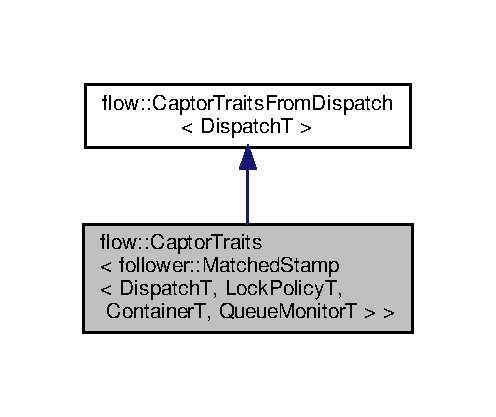
\includegraphics[width=238pt]{structflow_1_1_captor_traits_3_01follower_1_1_matched_stamp_3_01_dispatch_t_00_01_lock_policy_t_50e0b0ed57e7c81309757363a9faa475}
\end{center}
\end{figure}


Collaboration diagram for flow\+:\+:Captor\+Traits$<$ follower\+:\+:Matched\+Stamp$<$ DispatchT, Lock\+PolicyT, ContainerT, Queue\+MonitorT $>$ $>$\+:
\nopagebreak
\begin{figure}[H]
\begin{center}
\leavevmode
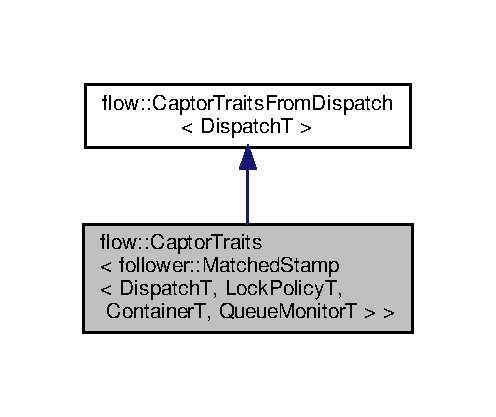
\includegraphics[width=238pt]{structflow_1_1_captor_traits_3_01follower_1_1_matched_stamp_3_01_dispatch_t_00_01_lock_policy_t_826efca46150488c4115be3a8705723b}
\end{center}
\end{figure}
\subsection*{Public Types}
\begin{DoxyCompactItemize}
\item 
\mbox{\Hypertarget{structflow_1_1_captor_traits_3_01follower_1_1_matched_stamp_3_01_dispatch_t_00_01_lock_policy_t_98530359aca39d952e431eb90b81d0f7_a582e956f60fbdaaac8140230c21ffd40}\label{structflow_1_1_captor_traits_3_01follower_1_1_matched_stamp_3_01_dispatch_t_00_01_lock_policy_t_98530359aca39d952e431eb90b81d0f7_a582e956f60fbdaaac8140230c21ffd40}} 
using \hyperlink{structflow_1_1_captor_traits_3_01follower_1_1_matched_stamp_3_01_dispatch_t_00_01_lock_policy_t_98530359aca39d952e431eb90b81d0f7_a582e956f60fbdaaac8140230c21ffd40}{Dispatch\+Container\+Type} = ContainerT
\begin{DoxyCompactList}\small\item\em Underlying dispatch container type. \end{DoxyCompactList}\item 
\mbox{\Hypertarget{structflow_1_1_captor_traits_3_01follower_1_1_matched_stamp_3_01_dispatch_t_00_01_lock_policy_t_98530359aca39d952e431eb90b81d0f7_a8ee6380548748ae7860e6c97399bc9c4}\label{structflow_1_1_captor_traits_3_01follower_1_1_matched_stamp_3_01_dispatch_t_00_01_lock_policy_t_98530359aca39d952e431eb90b81d0f7_a8ee6380548748ae7860e6c97399bc9c4}} 
using \hyperlink{structflow_1_1_captor_traits_3_01follower_1_1_matched_stamp_3_01_dispatch_t_00_01_lock_policy_t_98530359aca39d952e431eb90b81d0f7_a8ee6380548748ae7860e6c97399bc9c4}{Dispatch\+Queue\+Monitor\+Type} = Queue\+MonitorT
\begin{DoxyCompactList}\small\item\em Queue monitor/capture preconditioning type. \end{DoxyCompactList}\item 
\mbox{\Hypertarget{structflow_1_1_captor_traits_3_01follower_1_1_matched_stamp_3_01_dispatch_t_00_01_lock_policy_t_98530359aca39d952e431eb90b81d0f7_a244b0df9652da571b512b439bd6e6f0a}\label{structflow_1_1_captor_traits_3_01follower_1_1_matched_stamp_3_01_dispatch_t_00_01_lock_policy_t_98530359aca39d952e431eb90b81d0f7_a244b0df9652da571b512b439bd6e6f0a}} 
using \hyperlink{structflow_1_1_captor_traits_3_01follower_1_1_matched_stamp_3_01_dispatch_t_00_01_lock_policy_t_98530359aca39d952e431eb90b81d0f7_a244b0df9652da571b512b439bd6e6f0a}{Lock\+Policy\+Type} = Lock\+PolicyT
\begin{DoxyCompactList}\small\item\em Thread locking policy type. \end{DoxyCompactList}\end{DoxyCompactItemize}
\subsection*{Static Public Attributes}
\begin{DoxyCompactItemize}
\item 
static constexpr bool \hyperlink{structflow_1_1_captor_traits_3_01follower_1_1_matched_stamp_3_01_dispatch_t_00_01_lock_policy_t_98530359aca39d952e431eb90b81d0f7_a2f6333b98bb73715063d224f6a1a5a39}{is\+\_\+capture\+\_\+deterministic} = true
\end{DoxyCompactItemize}


\subsection{Detailed Description}
\subsubsection*{template$<$typename DispatchT, typename Lock\+PolicyT, typename ContainerT, typename Queue\+MonitorT$>$\newline
struct flow\+::\+Captor\+Traits$<$ follower\+::\+Matched\+Stamp$<$ Dispatch\+T, Lock\+Policy\+T, Container\+T, Queue\+Monitor\+T $>$ $>$}

Traits struct for captor types. 

Requires\+:
\begin{DoxyItemize}
\item {\ttfamily Dispatch\+Type} \+: data dispatch object type
\item {\ttfamily Dispatch\+Container\+Type} \+: container for {\ttfamily Dispatch\+Type} {\ttfamily Dispatch\+Queue\+Monitor\+Type} \+: optional monitoring/capture preconditioning object type
\item {\ttfamily value\+\_\+type} \+: data value type
\item {\ttfamily stamp\+\_\+type} \+: sequence stamp type
\item {\ttfamily size\+\_\+type} \+: integer sizing type
\end{DoxyItemize}


\begin{DoxyTemplParams}{Template Parameters}
{\em CaptorT} & captor type with C\+R\+TP base {\ttfamily \hyperlink{classflow_1_1_captor}{Captor}}\\
\hline
{\em DispatchT} & data dispatch type \\
\hline
{\em Lock\+PolicyT} & a Basic\+Lockable (\href{https://en.cppreference.com/w/cpp/named_req/BasicLockable}{\tt https\+://en.\+cppreference.\+com/w/cpp/named\+\_\+req/\+Basic\+Lockable}) object or \hyperlink{structflow_1_1_no_lock}{No\+Lock} or \hyperlink{structflow_1_1_polling_lock}{Polling\+Lock} \\
\hline
{\em ContainerT} & underlying {\ttfamily DispatchT} container type \\
\hline
{\em Queue\+MonitorT} & queue monitor/capture preconditioning type \\
\hline
\end{DoxyTemplParams}


\subsection{Member Data Documentation}
\mbox{\Hypertarget{structflow_1_1_captor_traits_3_01follower_1_1_matched_stamp_3_01_dispatch_t_00_01_lock_policy_t_98530359aca39d952e431eb90b81d0f7_a2f6333b98bb73715063d224f6a1a5a39}\label{structflow_1_1_captor_traits_3_01follower_1_1_matched_stamp_3_01_dispatch_t_00_01_lock_policy_t_98530359aca39d952e431eb90b81d0f7_a2f6333b98bb73715063d224f6a1a5a39}} 
\index{flow\+::\+Captor\+Traits$<$ follower\+::\+Matched\+Stamp$<$ Dispatch\+T, Lock\+Policy\+T, Container\+T, Queue\+Monitor\+T $>$ $>$@{flow\+::\+Captor\+Traits$<$ follower\+::\+Matched\+Stamp$<$ Dispatch\+T, Lock\+Policy\+T, Container\+T, Queue\+Monitor\+T $>$ $>$}!is\+\_\+capture\+\_\+deterministic@{is\+\_\+capture\+\_\+deterministic}}
\index{is\+\_\+capture\+\_\+deterministic@{is\+\_\+capture\+\_\+deterministic}!flow\+::\+Captor\+Traits$<$ follower\+::\+Matched\+Stamp$<$ Dispatch\+T, Lock\+Policy\+T, Container\+T, Queue\+Monitor\+T $>$ $>$@{flow\+::\+Captor\+Traits$<$ follower\+::\+Matched\+Stamp$<$ Dispatch\+T, Lock\+Policy\+T, Container\+T, Queue\+Monitor\+T $>$ $>$}}
\subsubsection{\texorpdfstring{is\+\_\+capture\+\_\+deterministic}{is\_capture\_deterministic}}
{\footnotesize\ttfamily template$<$typename DispatchT , typename Lock\+PolicyT , typename ContainerT , typename Queue\+MonitorT $>$ \\
constexpr bool \hyperlink{structflow_1_1_captor_traits}{flow\+::\+Captor\+Traits}$<$ \hyperlink{classflow_1_1follower_1_1_matched_stamp}{follower\+::\+Matched\+Stamp}$<$ DispatchT, Lock\+PolicyT, ContainerT, Queue\+MonitorT $>$ $>$\+::is\+\_\+capture\+\_\+deterministic = true\hspace{0.3cm}{\ttfamily [static]}}

Indicates that data from this captor will always be captured deterministically, so long as data injection is monotonically sequenced 

The documentation for this struct was generated from the following file\+:\begin{DoxyCompactItemize}
\item 
flow/include/follower/\hyperlink{matched__stamp_8h}{matched\+\_\+stamp.\+h}\end{DoxyCompactItemize}

\hypertarget{structflow_1_1_captor_traits_3_01follower_1_1_ranged_3_01_dispatch_t_00_01_lock_policy_t_00_01_c08104af94995091b5ab7569e730f476c}{}\section{flow\+:\+:Captor\+Traits$<$ follower\+:\+:Ranged$<$ DispatchT, Lock\+PolicyT, ContainerT, Queue\+MonitorT $>$ $>$ Struct Template Reference}
\label{structflow_1_1_captor_traits_3_01follower_1_1_ranged_3_01_dispatch_t_00_01_lock_policy_t_00_01_c08104af94995091b5ab7569e730f476c}\index{flow\+::\+Captor\+Traits$<$ follower\+::\+Ranged$<$ Dispatch\+T, Lock\+Policy\+T, Container\+T, Queue\+Monitor\+T $>$ $>$@{flow\+::\+Captor\+Traits$<$ follower\+::\+Ranged$<$ Dispatch\+T, Lock\+Policy\+T, Container\+T, Queue\+Monitor\+T $>$ $>$}}


Traits struct for captor types.  




{\ttfamily \#include $<$ranged.\+h$>$}



Inheritance diagram for flow\+:\+:Captor\+Traits$<$ follower\+:\+:Ranged$<$ DispatchT, Lock\+PolicyT, ContainerT, Queue\+MonitorT $>$ $>$\+:
\nopagebreak
\begin{figure}[H]
\begin{center}
\leavevmode
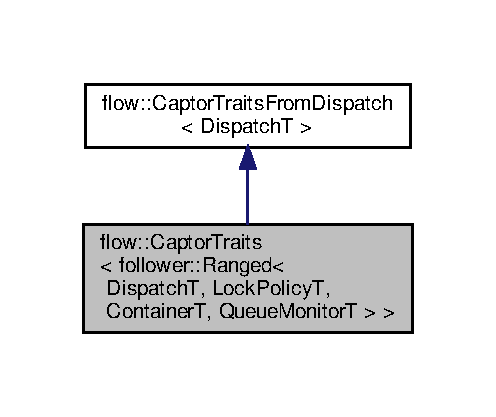
\includegraphics[width=238pt]{structflow_1_1_captor_traits_3_01follower_1_1_ranged_3_01_dispatch_t_00_01_lock_policy_t_00_01_cf0e94e7986d512f1273b0e82b06e4a0b}
\end{center}
\end{figure}


Collaboration diagram for flow\+:\+:Captor\+Traits$<$ follower\+:\+:Ranged$<$ DispatchT, Lock\+PolicyT, ContainerT, Queue\+MonitorT $>$ $>$\+:
\nopagebreak
\begin{figure}[H]
\begin{center}
\leavevmode
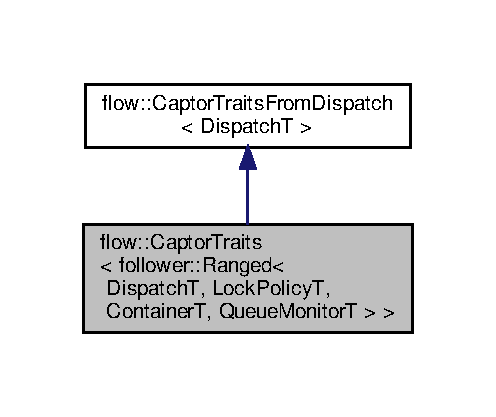
\includegraphics[width=238pt]{structflow_1_1_captor_traits_3_01follower_1_1_ranged_3_01_dispatch_t_00_01_lock_policy_t_00_01_cf2b572e9b9859067697e559bdb6043f1}
\end{center}
\end{figure}
\subsection*{Public Types}
\begin{DoxyCompactItemize}
\item 
\mbox{\Hypertarget{structflow_1_1_captor_traits_3_01follower_1_1_ranged_3_01_dispatch_t_00_01_lock_policy_t_00_01_c08104af94995091b5ab7569e730f476c_a662b69bc21ea01141af34c2fafd0a7b5}\label{structflow_1_1_captor_traits_3_01follower_1_1_ranged_3_01_dispatch_t_00_01_lock_policy_t_00_01_c08104af94995091b5ab7569e730f476c_a662b69bc21ea01141af34c2fafd0a7b5}} 
using \hyperlink{structflow_1_1_captor_traits_3_01follower_1_1_ranged_3_01_dispatch_t_00_01_lock_policy_t_00_01_c08104af94995091b5ab7569e730f476c_a662b69bc21ea01141af34c2fafd0a7b5}{Dispatch\+Container\+Type} = ContainerT
\begin{DoxyCompactList}\small\item\em Underlying dispatch container type. \end{DoxyCompactList}\item 
\mbox{\Hypertarget{structflow_1_1_captor_traits_3_01follower_1_1_ranged_3_01_dispatch_t_00_01_lock_policy_t_00_01_c08104af94995091b5ab7569e730f476c_a1b28b8d74c0e9d0cd69c75f08a9f4dea}\label{structflow_1_1_captor_traits_3_01follower_1_1_ranged_3_01_dispatch_t_00_01_lock_policy_t_00_01_c08104af94995091b5ab7569e730f476c_a1b28b8d74c0e9d0cd69c75f08a9f4dea}} 
using \hyperlink{structflow_1_1_captor_traits_3_01follower_1_1_ranged_3_01_dispatch_t_00_01_lock_policy_t_00_01_c08104af94995091b5ab7569e730f476c_a1b28b8d74c0e9d0cd69c75f08a9f4dea}{Dispatch\+Queue\+Monitor\+Type} = Queue\+MonitorT
\begin{DoxyCompactList}\small\item\em Queue monitor/capture preconditioning type. \end{DoxyCompactList}\item 
\mbox{\Hypertarget{structflow_1_1_captor_traits_3_01follower_1_1_ranged_3_01_dispatch_t_00_01_lock_policy_t_00_01_c08104af94995091b5ab7569e730f476c_afbbc4e6e1a4c8117fdb377bf52831081}\label{structflow_1_1_captor_traits_3_01follower_1_1_ranged_3_01_dispatch_t_00_01_lock_policy_t_00_01_c08104af94995091b5ab7569e730f476c_afbbc4e6e1a4c8117fdb377bf52831081}} 
using \hyperlink{structflow_1_1_captor_traits_3_01follower_1_1_ranged_3_01_dispatch_t_00_01_lock_policy_t_00_01_c08104af94995091b5ab7569e730f476c_afbbc4e6e1a4c8117fdb377bf52831081}{Lock\+Policy\+Type} = Lock\+PolicyT
\begin{DoxyCompactList}\small\item\em Thread locking policy type. \end{DoxyCompactList}\end{DoxyCompactItemize}
\subsection*{Static Public Attributes}
\begin{DoxyCompactItemize}
\item 
static constexpr bool \hyperlink{structflow_1_1_captor_traits_3_01follower_1_1_ranged_3_01_dispatch_t_00_01_lock_policy_t_00_01_c08104af94995091b5ab7569e730f476c_aed220dcf982664420a545dc0638eb0fc}{is\+\_\+capture\+\_\+deterministic} = true
\end{DoxyCompactItemize}


\subsection{Detailed Description}
\subsubsection*{template$<$typename DispatchT, typename Lock\+PolicyT, typename ContainerT, typename Queue\+MonitorT$>$\newline
struct flow\+::\+Captor\+Traits$<$ follower\+::\+Ranged$<$ Dispatch\+T, Lock\+Policy\+T, Container\+T, Queue\+Monitor\+T $>$ $>$}

Traits struct for captor types. 

Requires\+:
\begin{DoxyItemize}
\item {\ttfamily Dispatch\+Type} \+: data dispatch object type
\item {\ttfamily Dispatch\+Container\+Type} \+: container for {\ttfamily Dispatch\+Type} {\ttfamily Dispatch\+Queue\+Monitor\+Type} \+: optional monitoring/capture preconditioning object type
\item {\ttfamily value\+\_\+type} \+: data value type
\item {\ttfamily stamp\+\_\+type} \+: sequence stamp type
\item {\ttfamily size\+\_\+type} \+: integer sizing type
\end{DoxyItemize}


\begin{DoxyTemplParams}{Template Parameters}
{\em CaptorT} & captor type with C\+R\+TP base {\ttfamily \hyperlink{classflow_1_1_captor}{Captor}}\\
\hline
{\em DispatchT} & data dispatch type \\
\hline
{\em Lock\+PolicyT} & a Basic\+Lockable (\href{https://en.cppreference.com/w/cpp/named_req/BasicLockable}{\tt https\+://en.\+cppreference.\+com/w/cpp/named\+\_\+req/\+Basic\+Lockable}) object or \hyperlink{structflow_1_1_no_lock}{No\+Lock} or \hyperlink{structflow_1_1_polling_lock}{Polling\+Lock} \\
\hline
{\em ContainerT} & underlying {\ttfamily DispatchT} container type \\
\hline
{\em Queue\+MonitorT} & queue monitor/capture preconditioning type \\
\hline
\end{DoxyTemplParams}


\subsection{Member Data Documentation}
\mbox{\Hypertarget{structflow_1_1_captor_traits_3_01follower_1_1_ranged_3_01_dispatch_t_00_01_lock_policy_t_00_01_c08104af94995091b5ab7569e730f476c_aed220dcf982664420a545dc0638eb0fc}\label{structflow_1_1_captor_traits_3_01follower_1_1_ranged_3_01_dispatch_t_00_01_lock_policy_t_00_01_c08104af94995091b5ab7569e730f476c_aed220dcf982664420a545dc0638eb0fc}} 
\index{flow\+::\+Captor\+Traits$<$ follower\+::\+Ranged$<$ Dispatch\+T, Lock\+Policy\+T, Container\+T, Queue\+Monitor\+T $>$ $>$@{flow\+::\+Captor\+Traits$<$ follower\+::\+Ranged$<$ Dispatch\+T, Lock\+Policy\+T, Container\+T, Queue\+Monitor\+T $>$ $>$}!is\+\_\+capture\+\_\+deterministic@{is\+\_\+capture\+\_\+deterministic}}
\index{is\+\_\+capture\+\_\+deterministic@{is\+\_\+capture\+\_\+deterministic}!flow\+::\+Captor\+Traits$<$ follower\+::\+Ranged$<$ Dispatch\+T, Lock\+Policy\+T, Container\+T, Queue\+Monitor\+T $>$ $>$@{flow\+::\+Captor\+Traits$<$ follower\+::\+Ranged$<$ Dispatch\+T, Lock\+Policy\+T, Container\+T, Queue\+Monitor\+T $>$ $>$}}
\subsubsection{\texorpdfstring{is\+\_\+capture\+\_\+deterministic}{is\_capture\_deterministic}}
{\footnotesize\ttfamily template$<$typename DispatchT , typename Lock\+PolicyT , typename ContainerT , typename Queue\+MonitorT $>$ \\
constexpr bool \hyperlink{structflow_1_1_captor_traits}{flow\+::\+Captor\+Traits}$<$ \hyperlink{classflow_1_1follower_1_1_ranged}{follower\+::\+Ranged}$<$ DispatchT, Lock\+PolicyT, ContainerT, Queue\+MonitorT $>$ $>$\+::is\+\_\+capture\+\_\+deterministic = true\hspace{0.3cm}{\ttfamily [static]}}

Indicates that data from this captor will always be captured deterministically, so long as data injection is monotonically sequenced 

The documentation for this struct was generated from the following file\+:\begin{DoxyCompactItemize}
\item 
flow/include/follower/\hyperlink{ranged_8h}{ranged.\+h}\end{DoxyCompactItemize}

\hypertarget{structflow_1_1_captor_traits_3_01_follower_3_01_policy_t_01_4_01_4}{}\section{flow\+:\+:Captor\+Traits$<$ Follower$<$ PolicyT $>$ $>$ Struct Template Reference}
\label{structflow_1_1_captor_traits_3_01_follower_3_01_policy_t_01_4_01_4}\index{flow\+::\+Captor\+Traits$<$ Follower$<$ Policy\+T $>$ $>$@{flow\+::\+Captor\+Traits$<$ Follower$<$ Policy\+T $>$ $>$}}


Traits struct for captor types.  




{\ttfamily \#include $<$follower.\+h$>$}



Inheritance diagram for flow\+:\+:Captor\+Traits$<$ Follower$<$ PolicyT $>$ $>$\+:\nopagebreak
\begin{figure}[H]
\begin{center}
\leavevmode
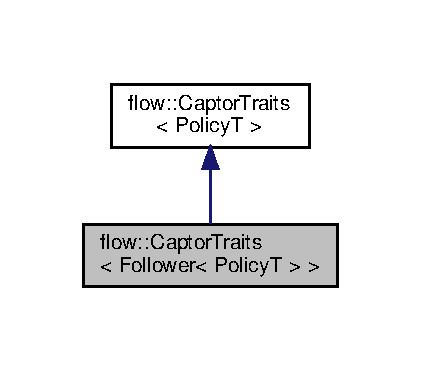
\includegraphics[width=202pt]{structflow_1_1_captor_traits_3_01_follower_3_01_policy_t_01_4_01_4__inherit__graph}
\end{center}
\end{figure}


Collaboration diagram for flow\+:\+:Captor\+Traits$<$ Follower$<$ PolicyT $>$ $>$\+:\nopagebreak
\begin{figure}[H]
\begin{center}
\leavevmode
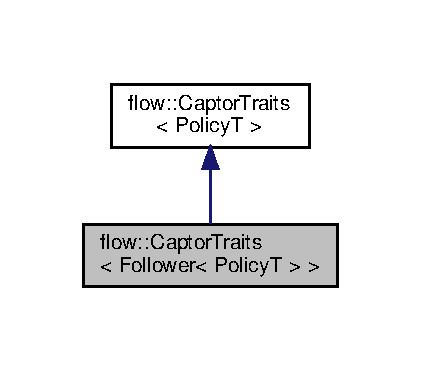
\includegraphics[width=202pt]{structflow_1_1_captor_traits_3_01_follower_3_01_policy_t_01_4_01_4__coll__graph}
\end{center}
\end{figure}


\subsection{Detailed Description}
\subsubsection*{template$<$typename PolicyT$>$\newline
struct flow\+::\+Captor\+Traits$<$ Follower$<$ Policy\+T $>$ $>$}

Traits struct for captor types. 

Requires\+:
\begin{DoxyItemize}
\item {\ttfamily Dispatch\+Type} \+: data dispatch object type
\item {\ttfamily Dispatch\+Container\+Type} \+: container for {\ttfamily Dispatch\+Type} {\ttfamily Dispatch\+Queue\+Monitor\+Type} \+: optional monitoring/capture preconditioning object type
\item {\ttfamily value\+\_\+type} \+: data value type
\item {\ttfamily stamp\+\_\+type} \+: sequence stamp type
\item {\ttfamily size\+\_\+type} \+: integer sizing type
\end{DoxyItemize}


\begin{DoxyTemplParams}{Template Parameters}
{\em CaptorT} & captor type with C\+R\+TP base {\ttfamily \hyperlink{classflow_1_1_captor}{Captor}} \\
\hline
{\em PolicyT} & C\+R\+T\+P-\/derived captor with specialized capture policy \\
\hline
\end{DoxyTemplParams}


The documentation for this struct was generated from the following file\+:\begin{DoxyCompactItemize}
\item 
flow/include/follower/\hyperlink{follower_8h}{follower.\+h}\end{DoxyCompactItemize}

\hypertarget{structflow_1_1_captor_traits_from_dispatch}{}\section{flow\+:\+:Captor\+Traits\+From\+Dispatch$<$ DispatchT $>$ Struct Template Reference}
\label{structflow_1_1_captor_traits_from_dispatch}\index{flow\+::\+Captor\+Traits\+From\+Dispatch$<$ Dispatch\+T $>$@{flow\+::\+Captor\+Traits\+From\+Dispatch$<$ Dispatch\+T $>$}}


Basic captor traits struct with common type information from data dispatch object.  




{\ttfamily \#include $<$captor.\+h$>$}



Inheritance diagram for flow\+:\+:Captor\+Traits\+From\+Dispatch$<$ DispatchT $>$\+:
\nopagebreak
\begin{figure}[H]
\begin{center}
\leavevmode
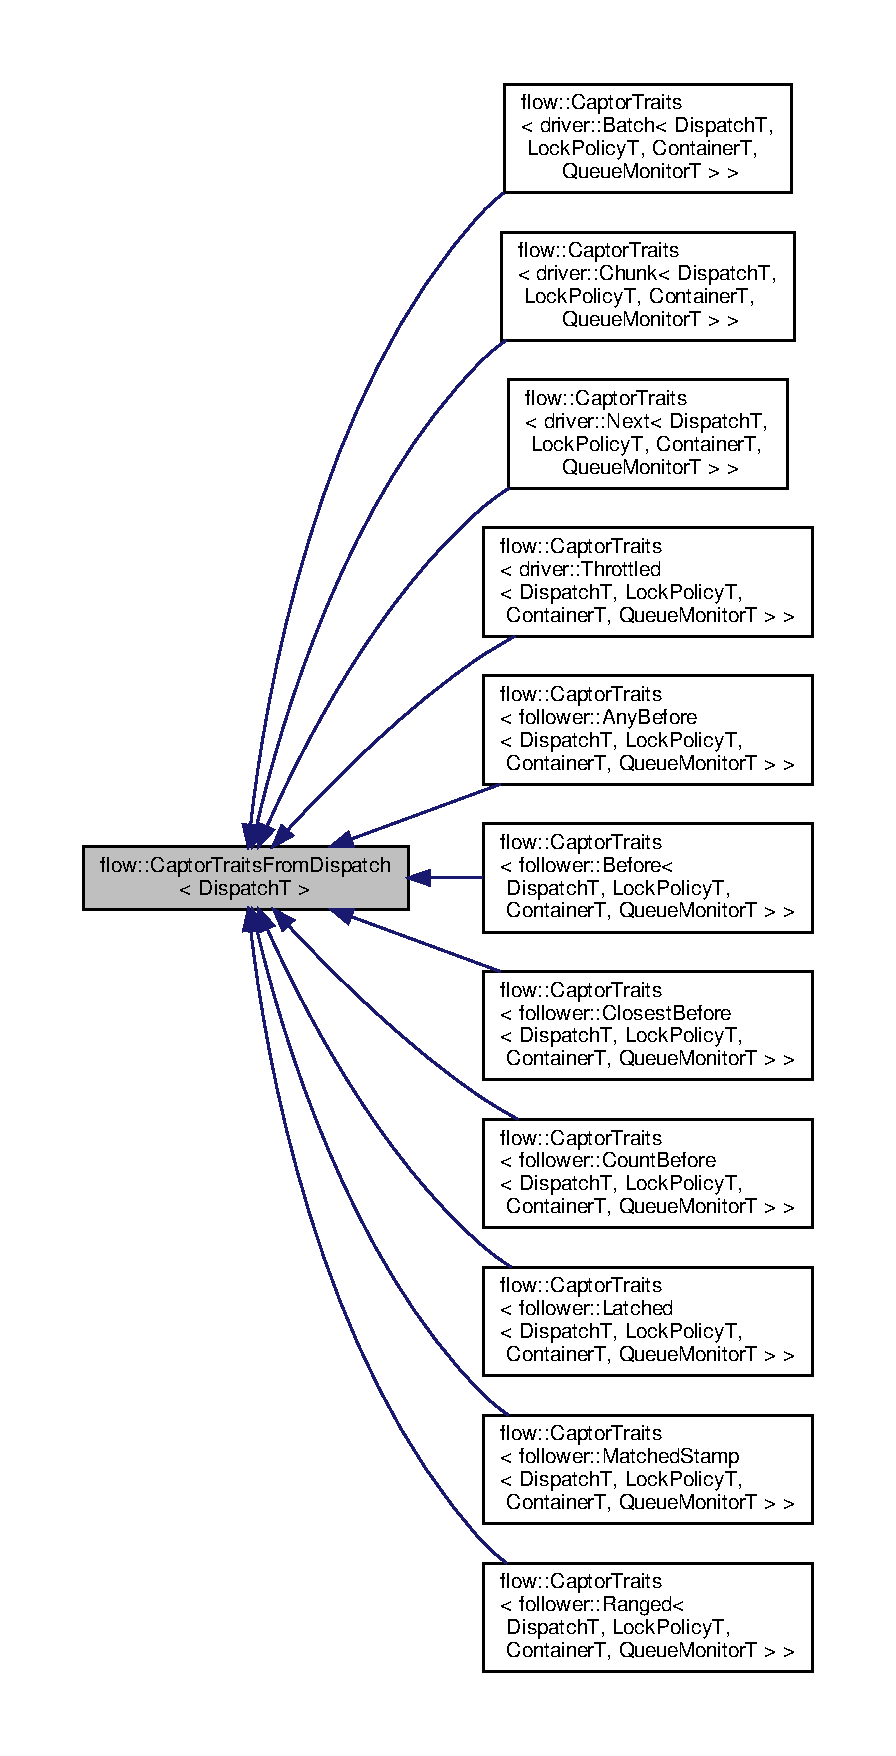
\includegraphics[height=550pt]{structflow_1_1_captor_traits_from_dispatch__inherit__graph}
\end{center}
\end{figure}
\subsection*{Public Types}
\begin{DoxyCompactItemize}
\item 
\mbox{\Hypertarget{structflow_1_1_captor_traits_from_dispatch_ab3ddf1794ab17bba478c020421d0ecb8}\label{structflow_1_1_captor_traits_from_dispatch_ab3ddf1794ab17bba478c020421d0ecb8}} 
using \hyperlink{structflow_1_1_captor_traits_from_dispatch_ab3ddf1794ab17bba478c020421d0ecb8}{Dispatch\+Type} = DispatchT
\begin{DoxyCompactList}\small\item\em \hyperlink{classflow_1_1_dispatch}{Dispatch} type. \end{DoxyCompactList}\item 
\mbox{\Hypertarget{structflow_1_1_captor_traits_from_dispatch_af9993a1c4d01b2884eef0f74720149b4}\label{structflow_1_1_captor_traits_from_dispatch_af9993a1c4d01b2884eef0f74720149b4}} 
using \hyperlink{structflow_1_1_captor_traits_from_dispatch_af9993a1c4d01b2884eef0f74720149b4}{value\+\_\+type} = typename \hyperlink{structflow_1_1_dispatch_traits}{Dispatch\+Traits}$<$ DispatchT $>$\+::\hyperlink{structflow_1_1_captor_traits_from_dispatch_af9993a1c4d01b2884eef0f74720149b4}{value\+\_\+type}
\begin{DoxyCompactList}\small\item\em \hyperlink{classflow_1_1_dispatch}{Dispatch} data value type. \end{DoxyCompactList}\item 
\mbox{\Hypertarget{structflow_1_1_captor_traits_from_dispatch_a33d283d578e545b1ce4c6c51b0b270f1}\label{structflow_1_1_captor_traits_from_dispatch_a33d283d578e545b1ce4c6c51b0b270f1}} 
using \hyperlink{structflow_1_1_captor_traits_from_dispatch_a33d283d578e545b1ce4c6c51b0b270f1}{stamp\+\_\+type} = typename \hyperlink{structflow_1_1_dispatch_traits}{Dispatch\+Traits}$<$ DispatchT $>$\+::\hyperlink{structflow_1_1_captor_traits_from_dispatch_a33d283d578e545b1ce4c6c51b0b270f1}{stamp\+\_\+type}
\begin{DoxyCompactList}\small\item\em \hyperlink{classflow_1_1_dispatch}{Dispatch} stamp type. \end{DoxyCompactList}\item 
\mbox{\Hypertarget{structflow_1_1_captor_traits_from_dispatch_a230ae2724dc491631b2e6806113b72b0}\label{structflow_1_1_captor_traits_from_dispatch_a230ae2724dc491631b2e6806113b72b0}} 
using \hyperlink{structflow_1_1_captor_traits_from_dispatch_a230ae2724dc491631b2e6806113b72b0}{offset\+\_\+type} = typename \hyperlink{structflow_1_1_stamp_traits}{Stamp\+Traits}$<$ \hyperlink{structflow_1_1_captor_traits_from_dispatch_a33d283d578e545b1ce4c6c51b0b270f1}{stamp\+\_\+type} $>$\+::\hyperlink{structflow_1_1_captor_traits_from_dispatch_a230ae2724dc491631b2e6806113b72b0}{offset\+\_\+type}
\begin{DoxyCompactList}\small\item\em Duration/offset type compatible with {\ttfamily stamp\+\_\+type} \end{DoxyCompactList}\item 
\mbox{\Hypertarget{structflow_1_1_captor_traits_from_dispatch_a27a621f56a740abb5fae3cfe8c4c1e88}\label{structflow_1_1_captor_traits_from_dispatch_a27a621f56a740abb5fae3cfe8c4c1e88}} 
using \hyperlink{structflow_1_1_captor_traits_from_dispatch_a27a621f56a740abb5fae3cfe8c4c1e88}{size\+\_\+type} = std\+::size\+\_\+t
\begin{DoxyCompactList}\small\item\em Integer size type. \end{DoxyCompactList}\end{DoxyCompactItemize}


\subsection{Detailed Description}
\subsubsection*{template$<$typename DispatchT$>$\newline
struct flow\+::\+Captor\+Traits\+From\+Dispatch$<$ Dispatch\+T $>$}

Basic captor traits struct with common type information from data dispatch object. 


\begin{DoxyTemplParams}{Template Parameters}
{\em DispatchT} & data dispatch object type \\
\hline
\end{DoxyTemplParams}


The documentation for this struct was generated from the following file\+:\begin{DoxyCompactItemize}
\item 
flow/include/\hyperlink{captor_8h}{captor.\+h}\end{DoxyCompactItemize}

\hypertarget{structflow_1_1_capture_range}{}\section{flow\+:\+:Capture\+Range$<$ StampT $>$ Struct Template Reference}
\label{structflow_1_1_capture_range}\index{flow\+::\+Capture\+Range$<$ Stamp\+T $>$@{flow\+::\+Capture\+Range$<$ Stamp\+T $>$}}


Data capture/sequencing information.  




{\ttfamily \#include $<$dispatch.\+h$>$}

\subsection*{Public Member Functions}
\begin{DoxyCompactItemize}
\item 
\hyperlink{structflow_1_1_capture_range_a525dd2f7119611ebdf7d02f2a5a15af9}{Capture\+Range} (const StampT \+\_\+lower\+\_\+stamp=\hyperlink{structflow_1_1_stamp_traits}{Stamp\+Traits}$<$ StampT $>$\+::max(), const StampT \+\_\+upper\+\_\+stamp=\hyperlink{structflow_1_1_stamp_traits}{Stamp\+Traits}$<$ StampT $>$\+::min())
\begin{DoxyCompactList}\small\item\em Sequencing range constructor. \end{DoxyCompactList}\item 
bool \hyperlink{structflow_1_1_capture_range_accdfed5d9a2410aed2a5e242b7d1335b}{valid} () const
\begin{DoxyCompactList}\small\item\em Checks if capture stamp range is valid. \end{DoxyCompactList}\item 
\hyperlink{structflow_1_1_capture_range_a9e48db61b83970a676a34c8af7bae594}{operator bool} () const
\begin{DoxyCompactList}\small\item\em Checks if capture stamp range is valid. \end{DoxyCompactList}\end{DoxyCompactItemize}
\subsection*{Public Attributes}
\begin{DoxyCompactItemize}
\item 
\mbox{\Hypertarget{structflow_1_1_capture_range_ab0f90a505b277b3ca9b1f72bd8097859}\label{structflow_1_1_capture_range_ab0f90a505b277b3ca9b1f72bd8097859}} 
StampT \hyperlink{structflow_1_1_capture_range_ab0f90a505b277b3ca9b1f72bd8097859}{lower\+\_\+stamp}
\begin{DoxyCompactList}\small\item\em Target sequence stamp produced from captured data associated with oldest captured element. \end{DoxyCompactList}\item 
\mbox{\Hypertarget{structflow_1_1_capture_range_a08e561c0c45af5a2890f00971a20b7f4}\label{structflow_1_1_capture_range_a08e561c0c45af5a2890f00971a20b7f4}} 
StampT \hyperlink{structflow_1_1_capture_range_a08e561c0c45af5a2890f00971a20b7f4}{upper\+\_\+stamp}
\begin{DoxyCompactList}\small\item\em Target sequence stamp produced from captured data associated with newest captured element. \end{DoxyCompactList}\end{DoxyCompactItemize}


\subsection{Detailed Description}
\subsubsection*{template$<$typename StampT$>$\newline
struct flow\+::\+Capture\+Range$<$ Stamp\+T $>$}

Data capture/sequencing information. 


\begin{DoxyTemplParams}{Template Parameters}
{\em StampT} & sequence stamp type \\
\hline
\end{DoxyTemplParams}


\subsection{Constructor \& Destructor Documentation}
\mbox{\Hypertarget{structflow_1_1_capture_range_a525dd2f7119611ebdf7d02f2a5a15af9}\label{structflow_1_1_capture_range_a525dd2f7119611ebdf7d02f2a5a15af9}} 
\index{flow\+::\+Capture\+Range@{flow\+::\+Capture\+Range}!Capture\+Range@{Capture\+Range}}
\index{Capture\+Range@{Capture\+Range}!flow\+::\+Capture\+Range@{flow\+::\+Capture\+Range}}
\subsubsection{\texorpdfstring{Capture\+Range()}{CaptureRange()}}
{\footnotesize\ttfamily template$<$typename StampT$>$ \\
\hyperlink{structflow_1_1_capture_range}{flow\+::\+Capture\+Range}$<$ StampT $>$\+::\hyperlink{structflow_1_1_capture_range}{Capture\+Range} (\begin{DoxyParamCaption}\item[{const StampT}]{\+\_\+lower\+\_\+stamp = {\ttfamily \hyperlink{structflow_1_1_stamp_traits}{Stamp\+Traits}$<$StampT$>$\+:\+:max()},  }\item[{const StampT}]{\+\_\+upper\+\_\+stamp = {\ttfamily \hyperlink{structflow_1_1_stamp_traits}{Stamp\+Traits}$<$StampT$>$\+:\+:min()} }\end{DoxyParamCaption})\hspace{0.3cm}{\ttfamily [inline]}}



Sequencing range constructor. 


\begin{DoxyParams}{Parameters}
{\em \+\_\+lower\+\_\+stamp} & lower sequencing stamp bound \\
\hline
{\em \+\_\+upper\+\_\+stamp} & upper sequencing stamp bound \\
\hline
\end{DoxyParams}


\subsection{Member Function Documentation}
\mbox{\Hypertarget{structflow_1_1_capture_range_a9e48db61b83970a676a34c8af7bae594}\label{structflow_1_1_capture_range_a9e48db61b83970a676a34c8af7bae594}} 
\index{flow\+::\+Capture\+Range@{flow\+::\+Capture\+Range}!operator bool@{operator bool}}
\index{operator bool@{operator bool}!flow\+::\+Capture\+Range@{flow\+::\+Capture\+Range}}
\subsubsection{\texorpdfstring{operator bool()}{operator bool()}}
{\footnotesize\ttfamily template$<$typename StampT$>$ \\
\hyperlink{structflow_1_1_capture_range}{flow\+::\+Capture\+Range}$<$ StampT $>$\+::operator bool (\begin{DoxyParamCaption}{ }\end{DoxyParamCaption}) const\hspace{0.3cm}{\ttfamily [inline]}}



Checks if capture stamp range is valid. 


\begin{DoxyRetVals}{Return values}
{\em true} & if upper\+\_\+stamp $>$= lower\+\_\+stamp \\
\hline
{\em false} & otherwise \\
\hline
\end{DoxyRetVals}
\mbox{\Hypertarget{structflow_1_1_capture_range_accdfed5d9a2410aed2a5e242b7d1335b}\label{structflow_1_1_capture_range_accdfed5d9a2410aed2a5e242b7d1335b}} 
\index{flow\+::\+Capture\+Range@{flow\+::\+Capture\+Range}!valid@{valid}}
\index{valid@{valid}!flow\+::\+Capture\+Range@{flow\+::\+Capture\+Range}}
\subsubsection{\texorpdfstring{valid()}{valid()}}
{\footnotesize\ttfamily template$<$typename StampT$>$ \\
bool \hyperlink{structflow_1_1_capture_range}{flow\+::\+Capture\+Range}$<$ StampT $>$\+::valid (\begin{DoxyParamCaption}{ }\end{DoxyParamCaption}) const\hspace{0.3cm}{\ttfamily [inline]}}



Checks if capture stamp range is valid. 


\begin{DoxyRetVals}{Return values}
{\em true} & if upper\+\_\+stamp $>$= lower\+\_\+stamp \\
\hline
{\em false} & otherwise \\
\hline
\end{DoxyRetVals}


The documentation for this struct was generated from the following file\+:\begin{DoxyCompactItemize}
\item 
flow/include/\hyperlink{dispatch_8h}{dispatch.\+h}\end{DoxyCompactItemize}

\hypertarget{classflow_1_1driver_1_1_chunk}{}\section{flow\+:\+:driver\+:\+:Chunk$<$ DispatchT, Lock\+PolicyT, ContainerT, Queue\+MonitorT $>$ Class Template Reference}
\label{classflow_1_1driver_1_1_chunk}\index{flow\+::driver\+::\+Chunk$<$ Dispatch\+T, Lock\+Policy\+T, Container\+T, Queue\+Monitor\+T $>$@{flow\+::driver\+::\+Chunk$<$ Dispatch\+T, Lock\+Policy\+T, Container\+T, Queue\+Monitor\+T $>$}}


Captures the next oldest data element.  




{\ttfamily \#include $<$chunk.\+h$>$}



Inheritance diagram for flow\+:\+:driver\+:\+:Chunk$<$ DispatchT, Lock\+PolicyT, ContainerT, Queue\+MonitorT $>$\+:
\nopagebreak
\begin{figure}[H]
\begin{center}
\leavevmode
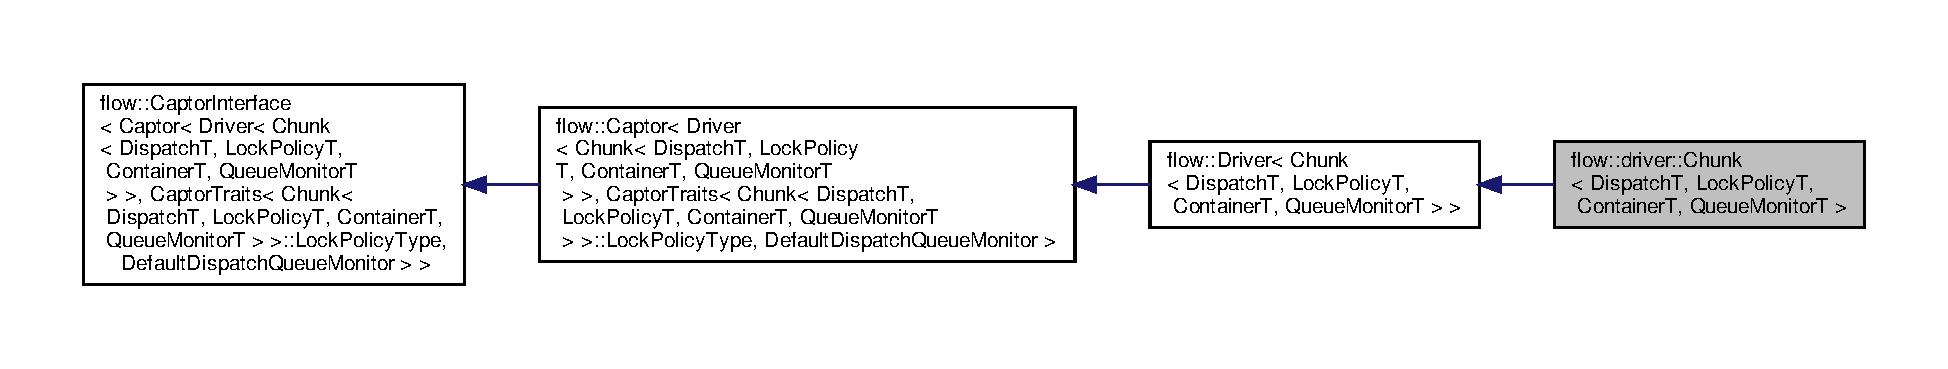
\includegraphics[width=350pt]{classflow_1_1driver_1_1_chunk__inherit__graph}
\end{center}
\end{figure}


Collaboration diagram for flow\+:\+:driver\+:\+:Chunk$<$ DispatchT, Lock\+PolicyT, ContainerT, Queue\+MonitorT $>$\+:
\nopagebreak
\begin{figure}[H]
\begin{center}
\leavevmode
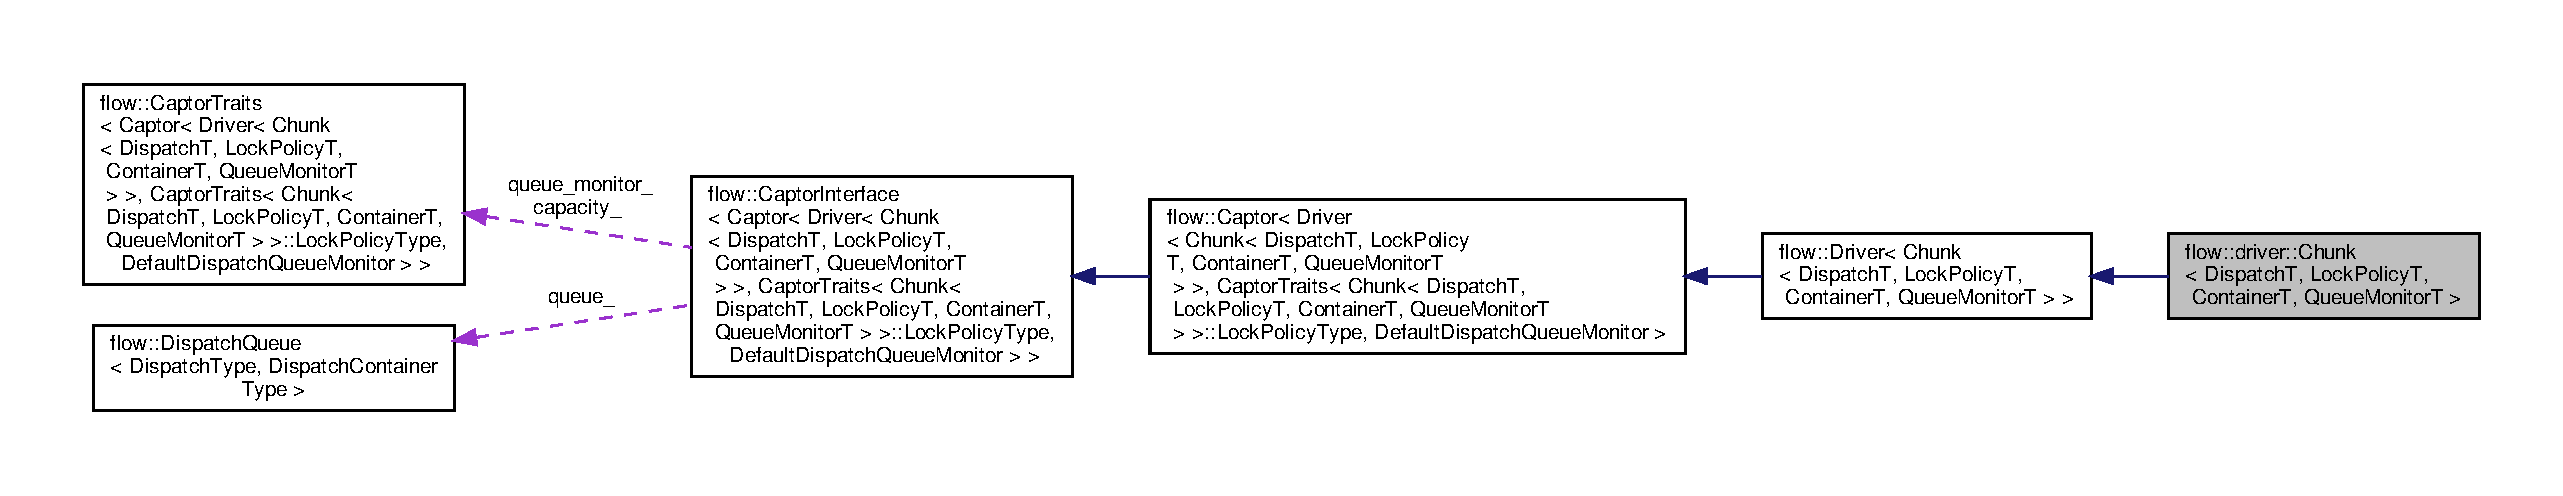
\includegraphics[width=350pt]{classflow_1_1driver_1_1_chunk__coll__graph}
\end{center}
\end{figure}
\subsection*{Public Types}
\begin{DoxyCompactItemize}
\item 
\mbox{\Hypertarget{classflow_1_1driver_1_1_chunk_ae04fbc608b52a2d35165e2ef95d742c3}\label{classflow_1_1driver_1_1_chunk_ae04fbc608b52a2d35165e2ef95d742c3}} 
using \hyperlink{classflow_1_1driver_1_1_chunk_ae04fbc608b52a2d35165e2ef95d742c3}{size\+\_\+type} = typename \hyperlink{structflow_1_1_captor_traits}{Captor\+Traits}$<$ \hyperlink{classflow_1_1driver_1_1_chunk}{Chunk} $>$\+::\hyperlink{classflow_1_1driver_1_1_chunk_ae04fbc608b52a2d35165e2ef95d742c3}{size\+\_\+type}
\begin{DoxyCompactList}\small\item\em Integer size type. \end{DoxyCompactList}\item 
\mbox{\Hypertarget{classflow_1_1driver_1_1_chunk_a6d8458f79fba18833a4893b09dd2937d}\label{classflow_1_1driver_1_1_chunk_a6d8458f79fba18833a4893b09dd2937d}} 
using \hyperlink{classflow_1_1driver_1_1_chunk_a6d8458f79fba18833a4893b09dd2937d}{stamp\+\_\+type} = typename \hyperlink{structflow_1_1_captor_traits}{Captor\+Traits}$<$ \hyperlink{classflow_1_1driver_1_1_chunk}{Chunk} $>$\+::\hyperlink{classflow_1_1driver_1_1_chunk_a6d8458f79fba18833a4893b09dd2937d}{stamp\+\_\+type}
\begin{DoxyCompactList}\small\item\em Data stamp type. \end{DoxyCompactList}\end{DoxyCompactItemize}
\subsection*{Public Member Functions}
\begin{DoxyCompactItemize}
\item 
\hyperlink{classflow_1_1driver_1_1_chunk_a19ef6ce723c1b2922b931471b835b627}{Chunk} (const \hyperlink{classflow_1_1driver_1_1_chunk_ae04fbc608b52a2d35165e2ef95d742c3}{size\+\_\+type} \hyperlink{classflow_1_1_captor_interface_a1a4b3f7f6c1bd16a2cb672d90a1cbbc0}{size}, const ContainerT \&container=ContainerT\{\}, const Queue\+MonitorT \&queue\+\_\+monitor=Queue\+MonitorT\{\}) noexcept(false)
\begin{DoxyCompactList}\small\item\em Configuration constructor. \end{DoxyCompactList}\end{DoxyCompactItemize}
\subsection*{Additional Inherited Members}


\subsection{Detailed Description}
\subsubsection*{template$<$typename DispatchT, typename Lock\+PolicyT = No\+Lock, typename ContainerT = Default\+Container$<$\+Dispatch\+T$>$, typename Queue\+MonitorT = Default\+Dispatch\+Queue\+Monitor$>$\newline
class flow\+::driver\+::\+Chunk$<$ Dispatch\+T, Lock\+Policy\+T, Container\+T, Queue\+Monitor\+T $>$}

Captures the next oldest data element. 

Establishes a sequencing range with where {\ttfamily range.\+lower\+\_\+stamp} is the stamp of the oldest captured element, and {\ttfamily range.\+upper\+\_\+stamp} is the stamp of the newest. Removes all captured elements from buffer.


\begin{DoxyTemplParams}{Template Parameters}
{\em DispatchT} & data dispatch type \\
\hline
{\em Lock\+PolicyT} & a Basic\+Lockable (\href{https://en.cppreference.com/w/cpp/named_req/BasicLockable}{\tt https\+://en.\+cppreference.\+com/w/cpp/named\+\_\+req/\+Basic\+Lockable}) object or \hyperlink{structflow_1_1_no_lock}{No\+Lock} or \hyperlink{structflow_1_1_polling_lock}{Polling\+Lock} \\
\hline
{\em ContainerT} & underlying {\ttfamily DispatchT} container type \\
\hline
{\em Queue\+MonitorT} & object used to monitor queue state on each insertion \\
\hline
\end{DoxyTemplParams}


\subsection{Constructor \& Destructor Documentation}
\mbox{\Hypertarget{classflow_1_1driver_1_1_chunk_a19ef6ce723c1b2922b931471b835b627}\label{classflow_1_1driver_1_1_chunk_a19ef6ce723c1b2922b931471b835b627}} 
\index{flow\+::driver\+::\+Chunk@{flow\+::driver\+::\+Chunk}!Chunk@{Chunk}}
\index{Chunk@{Chunk}!flow\+::driver\+::\+Chunk@{flow\+::driver\+::\+Chunk}}
\subsubsection{\texorpdfstring{Chunk()}{Chunk()}}
{\footnotesize\ttfamily template$<$typename DispatchT , typename Lock\+PolicyT  = No\+Lock, typename ContainerT  = Default\+Container$<$\+Dispatch\+T$>$, typename Queue\+MonitorT  = Default\+Dispatch\+Queue\+Monitor$>$ \\
\hyperlink{classflow_1_1driver_1_1_chunk}{flow\+::driver\+::\+Chunk}$<$ DispatchT, Lock\+PolicyT, ContainerT, Queue\+MonitorT $>$\+::\hyperlink{classflow_1_1driver_1_1_chunk}{Chunk} (\begin{DoxyParamCaption}\item[{const \hyperlink{classflow_1_1driver_1_1_chunk_ae04fbc608b52a2d35165e2ef95d742c3}{size\+\_\+type}}]{size,  }\item[{const ContainerT \&}]{container = {\ttfamily ContainerT\{\}},  }\item[{const Queue\+MonitorT \&}]{queue\+\_\+monitor = {\ttfamily QueueMonitorT\{\}} }\end{DoxyParamCaption})\hspace{0.3cm}{\ttfamily [explicit]}, {\ttfamily [noexcept]}}



Configuration constructor. 


\begin{DoxyParams}{Parameters}
{\em size} & number of elements to batch before becoming ready \\
\hline
{\em container} & container object with some initial state\\
\hline
\end{DoxyParams}

\begin{DoxyExceptions}{Exceptions}
{\em $<$code$>$std\+::invalid\+\_\+argument$<$/code$>$} & if {\ttfamily size == 0} \\
\hline
{\em $<$code$>$std\+::invalid\+\_\+argument$<$/code$>$} & if {\ttfamily Capture\+OutputT} cannot hold {\ttfamily size} \\
\hline
\end{DoxyExceptions}


The documentation for this class was generated from the following file\+:\begin{DoxyCompactItemize}
\item 
flow/include/driver/chunk.\+h\end{DoxyCompactItemize}

\hypertarget{classflow_1_1follower_1_1_closest_before}{}\section{flow\+:\+:follower\+:\+:Closest\+Before$<$ DispatchT, Lock\+PolicyT, ContainerT, Queue\+MonitorT $>$ Class Template Reference}
\label{classflow_1_1follower_1_1_closest_before}\index{flow\+::follower\+::\+Closest\+Before$<$ Dispatch\+T, Lock\+Policy\+T, Container\+T, Queue\+Monitor\+T $>$@{flow\+::follower\+::\+Closest\+Before$<$ Dispatch\+T, Lock\+Policy\+T, Container\+T, Queue\+Monitor\+T $>$}}


Captures one element before the capture range lower bound, minus a delay period, within an expected period.  




{\ttfamily \#include $<$closest\+\_\+before.\+h$>$}



Inheritance diagram for flow\+:\+:follower\+:\+:Closest\+Before$<$ DispatchT, Lock\+PolicyT, ContainerT, Queue\+MonitorT $>$\+:
\nopagebreak
\begin{figure}[H]
\begin{center}
\leavevmode
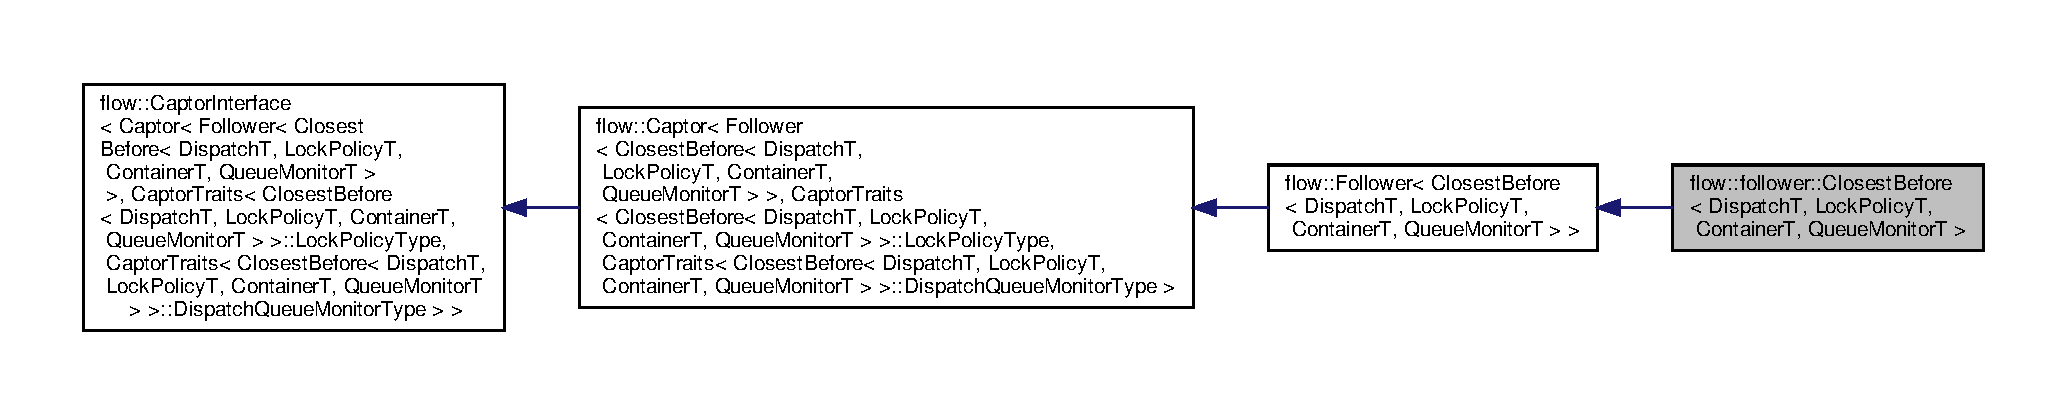
\includegraphics[width=350pt]{classflow_1_1follower_1_1_closest_before__inherit__graph}
\end{center}
\end{figure}


Collaboration diagram for flow\+:\+:follower\+:\+:Closest\+Before$<$ DispatchT, Lock\+PolicyT, ContainerT, Queue\+MonitorT $>$\+:
\nopagebreak
\begin{figure}[H]
\begin{center}
\leavevmode
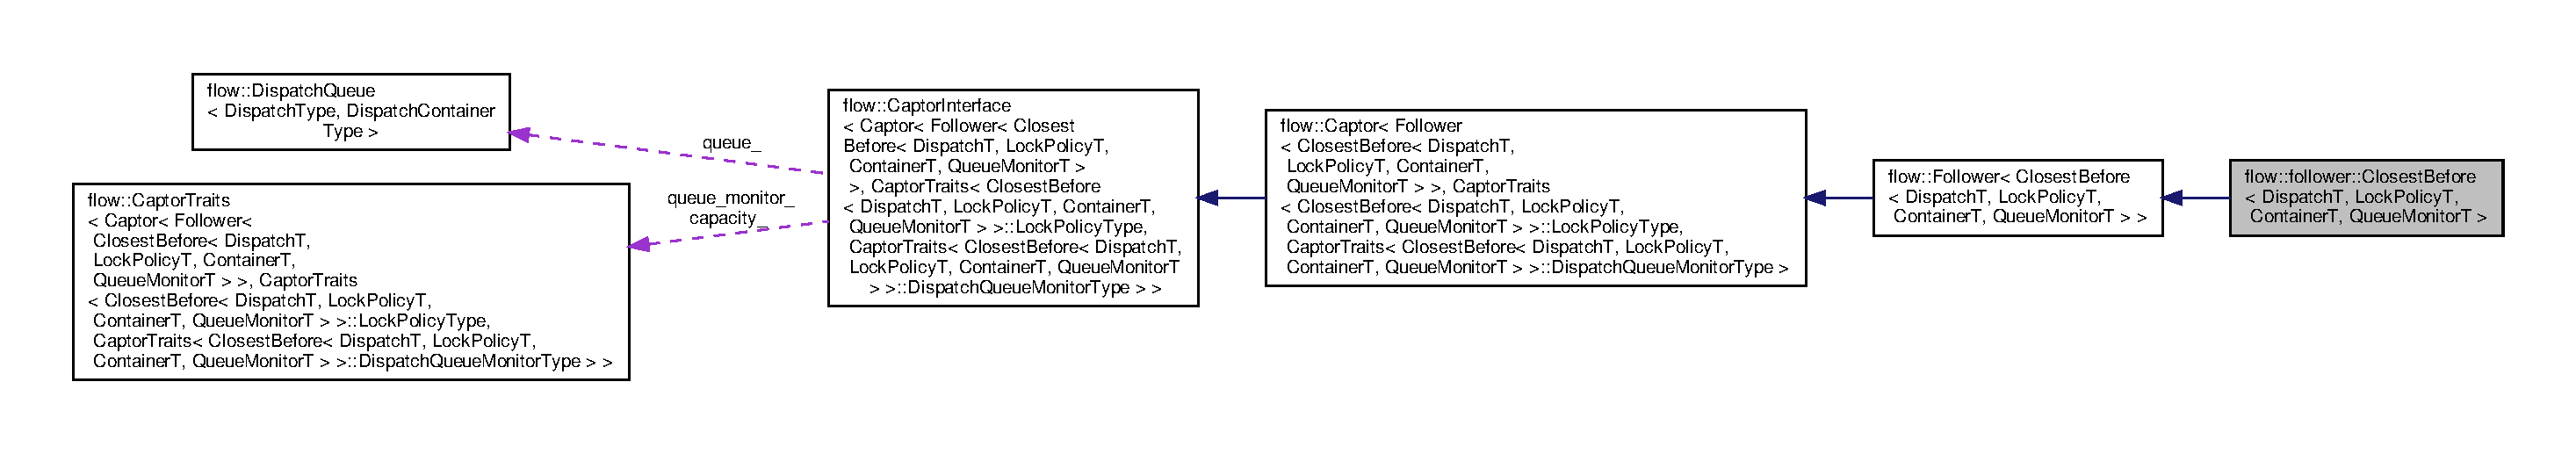
\includegraphics[width=350pt]{classflow_1_1follower_1_1_closest_before__coll__graph}
\end{center}
\end{figure}
\subsection*{Public Types}
\begin{DoxyCompactItemize}
\item 
\mbox{\Hypertarget{classflow_1_1follower_1_1_closest_before_af69e441e1ca309083983a6414cc606a2}\label{classflow_1_1follower_1_1_closest_before_af69e441e1ca309083983a6414cc606a2}} 
using \hyperlink{classflow_1_1follower_1_1_closest_before_af69e441e1ca309083983a6414cc606a2}{stamp\+\_\+type} = typename \hyperlink{structflow_1_1_captor_traits}{Captor\+Traits}$<$ \hyperlink{classflow_1_1follower_1_1_closest_before}{Closest\+Before} $>$\+::\hyperlink{classflow_1_1follower_1_1_closest_before_af69e441e1ca309083983a6414cc606a2}{stamp\+\_\+type}
\begin{DoxyCompactList}\small\item\em Data stamp type. \end{DoxyCompactList}\item 
\mbox{\Hypertarget{classflow_1_1follower_1_1_closest_before_ad6e3ed90bcd84a7948178e017ea9e79e}\label{classflow_1_1follower_1_1_closest_before_ad6e3ed90bcd84a7948178e017ea9e79e}} 
using \hyperlink{classflow_1_1follower_1_1_closest_before_ad6e3ed90bcd84a7948178e017ea9e79e}{offset\+\_\+type} = typename \hyperlink{structflow_1_1_captor_traits}{Captor\+Traits}$<$ \hyperlink{classflow_1_1follower_1_1_closest_before}{Closest\+Before} $>$\+::\hyperlink{classflow_1_1follower_1_1_closest_before_ad6e3ed90bcd84a7948178e017ea9e79e}{offset\+\_\+type}
\begin{DoxyCompactList}\small\item\em Data stamp duration type. \end{DoxyCompactList}\end{DoxyCompactItemize}
\subsection*{Public Member Functions}
\begin{DoxyCompactItemize}
\item 
\hyperlink{classflow_1_1follower_1_1_closest_before_ae09d7c8070e56939693f7cdfc6a720fc}{Closest\+Before} (const \hyperlink{classflow_1_1follower_1_1_closest_before_ad6e3ed90bcd84a7948178e017ea9e79e}{offset\+\_\+type} \&period, const \hyperlink{classflow_1_1follower_1_1_closest_before_ad6e3ed90bcd84a7948178e017ea9e79e}{offset\+\_\+type} \&delay, const ContainerT \&container=ContainerT\{\}, const Queue\+MonitorT \&queue\+\_\+monitor=Queue\+MonitorT\{\})
\begin{DoxyCompactList}\small\item\em Setup constructor. \end{DoxyCompactList}\end{DoxyCompactItemize}
\subsection*{Additional Inherited Members}


\subsection{Detailed Description}
\subsubsection*{template$<$typename DispatchT, typename Lock\+PolicyT = No\+Lock, typename ContainerT = Default\+Container$<$\+Dispatch\+T$>$, typename Queue\+MonitorT = Default\+Dispatch\+Queue\+Monitor$>$\newline
class flow\+::follower\+::\+Closest\+Before$<$ Dispatch\+T, Lock\+Policy\+T, Container\+T, Queue\+Monitor\+T $>$}

Captures one element before the capture range lower bound, minus a delay period, within an expected period. 

All older elements are removed.


\begin{DoxyTemplParams}{Template Parameters}
{\em DispatchT} & data dispatch type \\
\hline
{\em Lock\+PolicyT} & a Basic\+Lockable (\href{https://en.cppreference.com/w/cpp/named_req/BasicLockable}{\tt https\+://en.\+cppreference.\+com/w/cpp/named\+\_\+req/\+Basic\+Lockable}) object or \hyperlink{structflow_1_1_no_lock}{No\+Lock} or \hyperlink{structflow_1_1_polling_lock}{Polling\+Lock} \\
\hline
{\em ContainerT} & underlying {\ttfamily DispatchT} container type \\
\hline
{\em Queue\+MonitorT} & object used to monitor queue state on each insertion; used to precondition capture\\
\hline
\end{DoxyTemplParams}
\hyperlink{classflow_1_1follower_1_1_closest_before}{Closest\+Before} will behave non-\/deterministically if actual input period (difference between successive dispatch stamps) does not match the {\ttfamily period} argument specified on construction. For example, if {\ttfamily period} is too large, than multiple inputs could appear before the driving range, causing for different data on two or more iterations where the \char`\"{}latest\char`\"{} data was assumed to have been the same 

\subsection{Constructor \& Destructor Documentation}
\mbox{\Hypertarget{classflow_1_1follower_1_1_closest_before_ae09d7c8070e56939693f7cdfc6a720fc}\label{classflow_1_1follower_1_1_closest_before_ae09d7c8070e56939693f7cdfc6a720fc}} 
\index{flow\+::follower\+::\+Closest\+Before@{flow\+::follower\+::\+Closest\+Before}!Closest\+Before@{Closest\+Before}}
\index{Closest\+Before@{Closest\+Before}!flow\+::follower\+::\+Closest\+Before@{flow\+::follower\+::\+Closest\+Before}}
\subsubsection{\texorpdfstring{Closest\+Before()}{ClosestBefore()}}
{\footnotesize\ttfamily template$<$typename DispatchT , typename Lock\+PolicyT  = No\+Lock, typename ContainerT  = Default\+Container$<$\+Dispatch\+T$>$, typename Queue\+MonitorT  = Default\+Dispatch\+Queue\+Monitor$>$ \\
\hyperlink{classflow_1_1follower_1_1_closest_before}{flow\+::follower\+::\+Closest\+Before}$<$ DispatchT, Lock\+PolicyT, ContainerT, Queue\+MonitorT $>$\+::\hyperlink{classflow_1_1follower_1_1_closest_before}{Closest\+Before} (\begin{DoxyParamCaption}\item[{const \hyperlink{classflow_1_1follower_1_1_closest_before_ad6e3ed90bcd84a7948178e017ea9e79e}{offset\+\_\+type} \&}]{period,  }\item[{const \hyperlink{classflow_1_1follower_1_1_closest_before_ad6e3ed90bcd84a7948178e017ea9e79e}{offset\+\_\+type} \&}]{delay,  }\item[{const ContainerT \&}]{container = {\ttfamily ContainerT\{\}},  }\item[{const Queue\+MonitorT \&}]{queue\+\_\+monitor = {\ttfamily QueueMonitorT\{\}} }\end{DoxyParamCaption})}



Setup constructor. 


\begin{DoxyParams}{Parameters}
{\em period} & expected half-\/period between successive data elements \\
\hline
{\em delay} & the delay with which to capture \\
\hline
{\em container} & container object with some initial state \\
\hline
{\em queue\+\_\+monitor} & queue monitor with some initial state \\
\hline
\end{DoxyParams}


The documentation for this class was generated from the following file\+:\begin{DoxyCompactItemize}
\item 
flow/include/follower/\hyperlink{closest__before_8h}{closest\+\_\+before.\+h}\end{DoxyCompactItemize}

\hypertarget{classflow_1_1follower_1_1_count_before}{}\section{flow\+:\+:follower\+:\+:Count\+Before$<$ DispatchT, Lock\+PolicyT, ContainerT, Queue\+MonitorT $>$ Class Template Reference}
\label{classflow_1_1follower_1_1_count_before}\index{flow\+::follower\+::\+Count\+Before$<$ Dispatch\+T, Lock\+Policy\+T, Container\+T, Queue\+Monitor\+T $>$@{flow\+::follower\+::\+Count\+Before$<$ Dispatch\+T, Lock\+Policy\+T, Container\+T, Queue\+Monitor\+T $>$}}


Captures N-\/elements before the capture range lower bound, minus a delay period.  




{\ttfamily \#include $<$count\+\_\+before.\+h$>$}



Inheritance diagram for flow\+:\+:follower\+:\+:Count\+Before$<$ DispatchT, Lock\+PolicyT, ContainerT, Queue\+MonitorT $>$\+:
\nopagebreak
\begin{figure}[H]
\begin{center}
\leavevmode
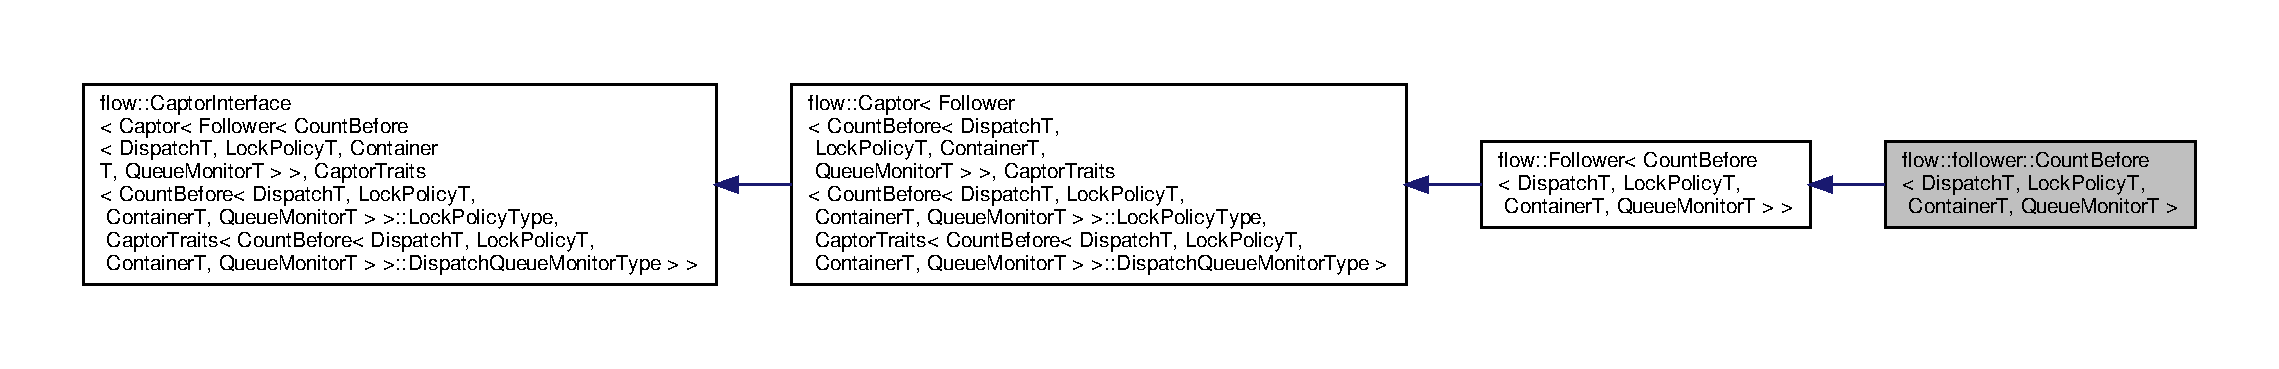
\includegraphics[width=350pt]{classflow_1_1follower_1_1_count_before__inherit__graph}
\end{center}
\end{figure}


Collaboration diagram for flow\+:\+:follower\+:\+:Count\+Before$<$ DispatchT, Lock\+PolicyT, ContainerT, Queue\+MonitorT $>$\+:
\nopagebreak
\begin{figure}[H]
\begin{center}
\leavevmode
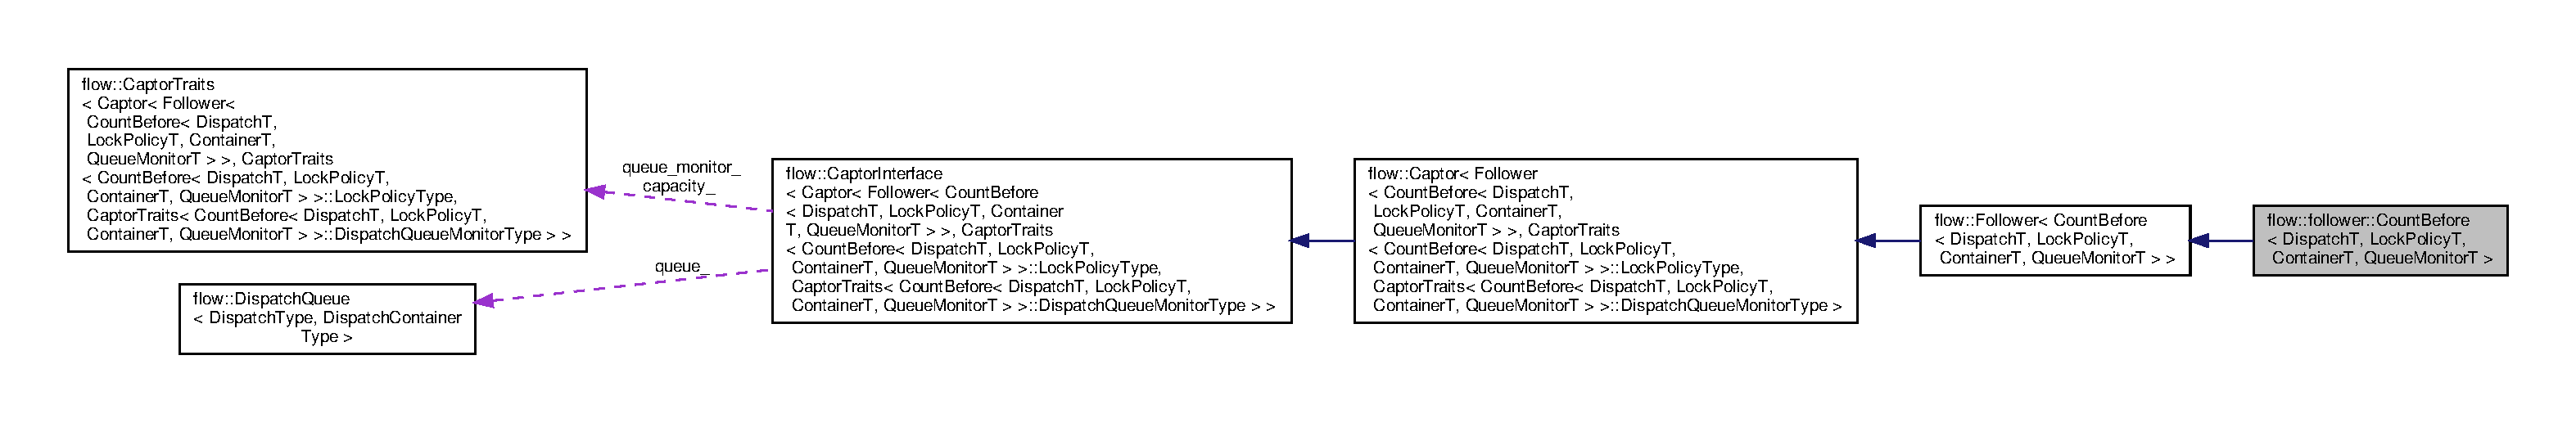
\includegraphics[width=350pt]{classflow_1_1follower_1_1_count_before__coll__graph}
\end{center}
\end{figure}
\subsection*{Public Types}
\begin{DoxyCompactItemize}
\item 
\mbox{\Hypertarget{classflow_1_1follower_1_1_count_before_a097b09f3a4af8a2a2772bfaddb00fdcc}\label{classflow_1_1follower_1_1_count_before_a097b09f3a4af8a2a2772bfaddb00fdcc}} 
using \hyperlink{classflow_1_1follower_1_1_count_before_a097b09f3a4af8a2a2772bfaddb00fdcc}{size\+\_\+type} = typename \hyperlink{structflow_1_1_captor_traits}{Captor\+Traits}$<$ \hyperlink{classflow_1_1follower_1_1_count_before}{Count\+Before} $>$\+::\hyperlink{classflow_1_1follower_1_1_count_before_a097b09f3a4af8a2a2772bfaddb00fdcc}{size\+\_\+type}
\begin{DoxyCompactList}\small\item\em Integer size type. \end{DoxyCompactList}\item 
\mbox{\Hypertarget{classflow_1_1follower_1_1_count_before_a9d39e5e485167849767fc463986525a6}\label{classflow_1_1follower_1_1_count_before_a9d39e5e485167849767fc463986525a6}} 
using \hyperlink{classflow_1_1follower_1_1_count_before_a9d39e5e485167849767fc463986525a6}{stamp\+\_\+type} = typename \hyperlink{structflow_1_1_captor_traits}{Captor\+Traits}$<$ \hyperlink{classflow_1_1follower_1_1_count_before}{Count\+Before} $>$\+::\hyperlink{classflow_1_1follower_1_1_count_before_a9d39e5e485167849767fc463986525a6}{stamp\+\_\+type}
\begin{DoxyCompactList}\small\item\em Data stamp type. \end{DoxyCompactList}\item 
\mbox{\Hypertarget{classflow_1_1follower_1_1_count_before_a99a0abf1a1d75aad7a5b1958f527f0a8}\label{classflow_1_1follower_1_1_count_before_a99a0abf1a1d75aad7a5b1958f527f0a8}} 
using \hyperlink{classflow_1_1follower_1_1_count_before_a99a0abf1a1d75aad7a5b1958f527f0a8}{offset\+\_\+type} = typename \hyperlink{structflow_1_1_captor_traits}{Captor\+Traits}$<$ \hyperlink{classflow_1_1follower_1_1_count_before}{Count\+Before} $>$\+::\hyperlink{classflow_1_1follower_1_1_count_before_a99a0abf1a1d75aad7a5b1958f527f0a8}{offset\+\_\+type}
\begin{DoxyCompactList}\small\item\em Data stamp duration type. \end{DoxyCompactList}\end{DoxyCompactItemize}
\subsection*{Public Member Functions}
\begin{DoxyCompactItemize}
\item 
\hyperlink{classflow_1_1follower_1_1_count_before_a0fdc19c152e8fc8f5ad9dc3fd23af265}{Count\+Before} (const \hyperlink{classflow_1_1follower_1_1_count_before_a097b09f3a4af8a2a2772bfaddb00fdcc}{size\+\_\+type} count, const \hyperlink{classflow_1_1follower_1_1_count_before_a99a0abf1a1d75aad7a5b1958f527f0a8}{offset\+\_\+type} \&delay, const ContainerT \&container=ContainerT\{\}, const Queue\+MonitorT \&queue\+\_\+monitor=Queue\+MonitorT\{\})
\begin{DoxyCompactList}\small\item\em Setup constructor. \end{DoxyCompactList}\end{DoxyCompactItemize}
\subsection*{Additional Inherited Members}


\subsection{Detailed Description}
\subsubsection*{template$<$typename DispatchT, typename Lock\+PolicyT = No\+Lock, typename ContainerT = Default\+Container$<$\+Dispatch\+T$>$, typename Queue\+MonitorT = Default\+Dispatch\+Queue\+Monitor$>$\newline
class flow\+::follower\+::\+Count\+Before$<$ Dispatch\+T, Lock\+Policy\+T, Container\+T, Queue\+Monitor\+T $>$}

Captures N-\/elements before the capture range lower bound, minus a delay period. 

All older elements are removed.


\begin{DoxyTemplParams}{Template Parameters}
{\em DispatchT} & data dispatch type \\
\hline
{\em Lock\+PolicyT} & a Basic\+Lockable (\href{https://en.cppreference.com/w/cpp/named_req/BasicLockable}{\tt https\+://en.\+cppreference.\+com/w/cpp/named\+\_\+req/\+Basic\+Lockable}) object or \hyperlink{structflow_1_1_no_lock}{No\+Lock} or \hyperlink{structflow_1_1_polling_lock}{Polling\+Lock} \\
\hline
{\em ContainerT} & underlying {\ttfamily DispatchT} container type \\
\hline
{\em Queue\+MonitorT} & object used to monitor queue state on each insertion; used to precondition capture \\
\hline
\end{DoxyTemplParams}


\subsection{Constructor \& Destructor Documentation}
\mbox{\Hypertarget{classflow_1_1follower_1_1_count_before_a0fdc19c152e8fc8f5ad9dc3fd23af265}\label{classflow_1_1follower_1_1_count_before_a0fdc19c152e8fc8f5ad9dc3fd23af265}} 
\index{flow\+::follower\+::\+Count\+Before@{flow\+::follower\+::\+Count\+Before}!Count\+Before@{Count\+Before}}
\index{Count\+Before@{Count\+Before}!flow\+::follower\+::\+Count\+Before@{flow\+::follower\+::\+Count\+Before}}
\subsubsection{\texorpdfstring{Count\+Before()}{CountBefore()}}
{\footnotesize\ttfamily template$<$typename DispatchT , typename Lock\+PolicyT  = No\+Lock, typename ContainerT  = Default\+Container$<$\+Dispatch\+T$>$, typename Queue\+MonitorT  = Default\+Dispatch\+Queue\+Monitor$>$ \\
\hyperlink{classflow_1_1follower_1_1_count_before}{flow\+::follower\+::\+Count\+Before}$<$ DispatchT, Lock\+PolicyT, ContainerT, Queue\+MonitorT $>$\+::\hyperlink{classflow_1_1follower_1_1_count_before}{Count\+Before} (\begin{DoxyParamCaption}\item[{const \hyperlink{classflow_1_1follower_1_1_count_before_a097b09f3a4af8a2a2772bfaddb00fdcc}{size\+\_\+type}}]{count,  }\item[{const \hyperlink{classflow_1_1follower_1_1_count_before_a99a0abf1a1d75aad7a5b1958f527f0a8}{offset\+\_\+type} \&}]{delay,  }\item[{const ContainerT \&}]{container = {\ttfamily ContainerT\{\}},  }\item[{const Queue\+MonitorT \&}]{queue\+\_\+monitor = {\ttfamily QueueMonitorT\{\}} }\end{DoxyParamCaption})}



Setup constructor. 


\begin{DoxyParams}{Parameters}
{\em count} & number of elements before to capture \\
\hline
{\em delay} & the delay with which to capture \\
\hline
{\em container} & container object with some initial state \\
\hline
{\em queue\+\_\+monitor} & queue monitor with some initial state\\
\hline
\end{DoxyParams}

\begin{DoxyExceptions}{Exceptions}
{\em $<$code$>$std\+::invalid\+\_\+argument$<$/code$>$} & if {\ttfamily count == 0} \\
\hline
\end{DoxyExceptions}


The documentation for this class was generated from the following file\+:\begin{DoxyCompactItemize}
\item 
flow/include/follower/\hyperlink{count__before_8h}{count\+\_\+before.\+h}\end{DoxyCompactItemize}

\hypertarget{structflow_1_1_default_dispatch_queue_monitor}{}\section{flow\+:\+:Default\+Dispatch\+Queue\+Monitor Struct Reference}
\label{structflow_1_1_default_dispatch_queue_monitor}\index{flow\+::\+Default\+Dispatch\+Queue\+Monitor@{flow\+::\+Default\+Dispatch\+Queue\+Monitor}}


Stand-\/in type used to replace queue monitor.  




{\ttfamily \#include $<$captor.\+h$>$}

\subsection*{Static Public Member Functions}
\begin{DoxyCompactItemize}
\item 
{\footnotesize template$<$typename DispatchT , typename Dispatch\+ContainerT , typename StampT $>$ }\\static constexpr bool \hyperlink{structflow_1_1_default_dispatch_queue_monitor_aed3f0234eeb6d3c60043d9d36047301a}{check} (\hyperlink{classflow_1_1_dispatch_queue}{Dispatch\+Queue}$<$ DispatchT, Dispatch\+ContainerT $>$ \&, const \hyperlink{structflow_1_1_capture_range}{Capture\+Range}$<$ StampT $>$ \&)
\begin{DoxyCompactList}\small\item\em Check queue monitor state with on capture attempt. \end{DoxyCompactList}\item 
{\footnotesize template$<$typename DispatchT , typename Dispatch\+ContainerT , typename StampT $>$ }\\static constexpr void \hyperlink{structflow_1_1_default_dispatch_queue_monitor_acccd20e4a17462c3d8d14e0aa26d1982}{update} (\hyperlink{classflow_1_1_dispatch_queue}{Dispatch\+Queue}$<$ DispatchT, Dispatch\+ContainerT $>$ \&, const \hyperlink{structflow_1_1_capture_range}{Capture\+Range}$<$ StampT $>$ \&, const \hyperlink{namespaceflow_adefe9726e597eb50c46f0f6a202018e9}{State})
\begin{DoxyCompactList}\small\item\em Updates queue monitor state with global synchronization results. \end{DoxyCompactList}\end{DoxyCompactItemize}


\subsection{Detailed Description}
Stand-\/in type used to replace queue monitor. 

\subsection{Member Function Documentation}
\mbox{\Hypertarget{structflow_1_1_default_dispatch_queue_monitor_aed3f0234eeb6d3c60043d9d36047301a}\label{structflow_1_1_default_dispatch_queue_monitor_aed3f0234eeb6d3c60043d9d36047301a}} 
\index{flow\+::\+Default\+Dispatch\+Queue\+Monitor@{flow\+::\+Default\+Dispatch\+Queue\+Monitor}!check@{check}}
\index{check@{check}!flow\+::\+Default\+Dispatch\+Queue\+Monitor@{flow\+::\+Default\+Dispatch\+Queue\+Monitor}}
\subsubsection{\texorpdfstring{check()}{check()}}
{\footnotesize\ttfamily template$<$typename DispatchT , typename Dispatch\+ContainerT , typename StampT $>$ \\
static constexpr bool flow\+::\+Default\+Dispatch\+Queue\+Monitor\+::check (\begin{DoxyParamCaption}\item[{\hyperlink{classflow_1_1_dispatch_queue}{Dispatch\+Queue}$<$ DispatchT, Dispatch\+ContainerT $>$ \&}]{,  }\item[{const \hyperlink{structflow_1_1_capture_range}{Capture\+Range}$<$ StampT $>$ \&}]{ }\end{DoxyParamCaption})\hspace{0.3cm}{\ttfamily [inline]}, {\ttfamily [static]}}



Check queue monitor state with on capture attempt. 

Checks are applied in \hyperlink{classflow_1_1_follower}{Follower} derivative \hyperlink{classflow_1_1_captor}{Captor} objects, only


\begin{DoxyRetVals}{Return values}
{\em true} & allows capture to happen \\
\hline
{\em false} & otherwise, causing \hyperlink{classflow_1_1_captor}{Captor} to return {\ttfamily \hyperlink{namespaceflow_adefe9726e597eb50c46f0f6a202018e9a553bb3189571a5b09c1d53c315abd8f8}{State\+::\+S\+K\+I\+P\+\_\+\+F\+R\+A\+M\+E\+\_\+\+Q\+U\+E\+U\+E\+\_\+\+P\+R\+E\+C\+O\+N\+D\+I\+T\+I\+ON}} \\
\hline
\end{DoxyRetVals}
\mbox{\Hypertarget{structflow_1_1_default_dispatch_queue_monitor_acccd20e4a17462c3d8d14e0aa26d1982}\label{structflow_1_1_default_dispatch_queue_monitor_acccd20e4a17462c3d8d14e0aa26d1982}} 
\index{flow\+::\+Default\+Dispatch\+Queue\+Monitor@{flow\+::\+Default\+Dispatch\+Queue\+Monitor}!update@{update}}
\index{update@{update}!flow\+::\+Default\+Dispatch\+Queue\+Monitor@{flow\+::\+Default\+Dispatch\+Queue\+Monitor}}
\subsubsection{\texorpdfstring{update()}{update()}}
{\footnotesize\ttfamily template$<$typename DispatchT , typename Dispatch\+ContainerT , typename StampT $>$ \\
static constexpr void flow\+::\+Default\+Dispatch\+Queue\+Monitor\+::update (\begin{DoxyParamCaption}\item[{\hyperlink{classflow_1_1_dispatch_queue}{Dispatch\+Queue}$<$ DispatchT, Dispatch\+ContainerT $>$ \&}]{,  }\item[{const \hyperlink{structflow_1_1_capture_range}{Capture\+Range}$<$ StampT $>$ \&}]{,  }\item[{const \hyperlink{namespaceflow_adefe9726e597eb50c46f0f6a202018e9}{State}}]{ }\end{DoxyParamCaption})\hspace{0.3cm}{\ttfamily [inline]}, {\ttfamily [static]}}



Updates queue monitor state with global synchronization results. 

Called during {\ttfamily Sychronizer\+::capture}, updating several associated \hyperlink{classflow_1_1_captor}{Captor} s 

The documentation for this struct was generated from the following file\+:\begin{DoxyCompactItemize}
\item 
flow/include/\hyperlink{captor_8h}{captor.\+h}\end{DoxyCompactItemize}

\hypertarget{classflow_1_1_dispatch}{}\section{flow\+:\+:Dispatch$<$ StampT, ValueT $>$ Class Template Reference}
\label{classflow_1_1_dispatch}\index{flow\+::\+Dispatch$<$ Stamp\+T, Value\+T $>$@{flow\+::\+Dispatch$<$ Stamp\+T, Value\+T $>$}}


\hyperlink{classflow_1_1_dispatch}{Dispatch} data wrapper.  




{\ttfamily \#include $<$dispatch.\+h$>$}

\subsection*{Public Member Functions}
\begin{DoxyCompactItemize}
\item 
\mbox{\Hypertarget{classflow_1_1_dispatch_a1131f6fb814e7f4ac55108c9971f19cf}\label{classflow_1_1_dispatch_a1131f6fb814e7f4ac55108c9971f19cf}} 
{\footnotesize template$<$typename... Value\+Args\+Ts$>$ }\\\hyperlink{classflow_1_1_dispatch_a1131f6fb814e7f4ac55108c9971f19cf}{Dispatch} (const StampT \&\+\_\+stamp, Value\+Args\+Ts \&\&... \+\_\+value\+\_\+args)
\begin{DoxyCompactList}\small\item\em \hyperlink{classflow_1_1_dispatch}{Dispatch} value constructor (move enabled) \end{DoxyCompactList}\end{DoxyCompactItemize}
\subsection*{Public Attributes}
\begin{DoxyCompactItemize}
\item 
\mbox{\Hypertarget{classflow_1_1_dispatch_aba36922397c417ba5da2858327463732}\label{classflow_1_1_dispatch_aba36922397c417ba5da2858327463732}} 
StampT \hyperlink{classflow_1_1_dispatch_aba36922397c417ba5da2858327463732}{stamp}
\begin{DoxyCompactList}\small\item\em Sequencing stamp associated with data. \end{DoxyCompactList}\item 
\mbox{\Hypertarget{classflow_1_1_dispatch_ae4a044a9ec7c77362bfac2319faa0652}\label{classflow_1_1_dispatch_ae4a044a9ec7c77362bfac2319faa0652}} 
ValueT \hyperlink{classflow_1_1_dispatch_ae4a044a9ec7c77362bfac2319faa0652}{value}
\begin{DoxyCompactList}\small\item\em Data element. \end{DoxyCompactList}\end{DoxyCompactItemize}


\subsection{Detailed Description}
\subsubsection*{template$<$typename StampT, typename ValueT$>$\newline
class flow\+::\+Dispatch$<$ Stamp\+T, Value\+T $>$}

\hyperlink{classflow_1_1_dispatch}{Dispatch} data wrapper. 

Custom \char`\"{}dispatching\char`\"{} objects may be used with this library in lieu of the standard {\ttfamily \hyperlink{classflow_1_1_dispatch}{Dispatch}} template provided in this file ~\newline
 Custom dispatch types must also specialize the {\ttfamily \hyperlink{structflow_1_1_dispatch_traits}{Dispatch\+Traits}} helper struct, which is used to provide core {\ttfamily stamp\+\_\+type} and {\ttfamily value\+\_\+type} to other dependent objects throughout the library.


\begin{DoxyTemplParams}{Template Parameters}
{\em StampT} & sequencing stamp type; used for data ordering (e.\+g. time, sequence number, etc.) \\
\hline
{\em ValueT} & data value type; must be copyable \\
\hline
\end{DoxyTemplParams}


The documentation for this class was generated from the following file\+:\begin{DoxyCompactItemize}
\item 
flow/include/\hyperlink{dispatch_8h}{dispatch.\+h}\end{DoxyCompactItemize}

\hypertarget{structflow_1_1_dispatch_access}{}\section{flow\+:\+:Dispatch\+Access$<$ DispatchT $>$ Struct Template Reference}
\label{structflow_1_1_dispatch_access}\index{flow\+::\+Dispatch\+Access$<$ Dispatch\+T $>$@{flow\+::\+Dispatch\+Access$<$ Dispatch\+T $>$}}


\hyperlink{classflow_1_1_dispatch}{Dispatch} access helper.  




{\ttfamily \#include $<$dispatch.\+h$>$}



\subsection{Detailed Description}
\subsubsection*{template$<$typename DispatchT$>$\newline
struct flow\+::\+Dispatch\+Access$<$ Dispatch\+T $>$}

\hyperlink{classflow_1_1_dispatch}{Dispatch} access helper. 

The documentation for this struct was generated from the following file\+:\begin{DoxyCompactItemize}
\item 
flow/include/\hyperlink{dispatch_8h}{dispatch.\+h}\end{DoxyCompactItemize}

\hypertarget{structflow_1_1_dispatch_access_3_01_dispatch_3_01_stamp_t_00_01_value_t_01_4_01_4}{}\section{flow\+:\+:Dispatch\+Access$<$ Dispatch$<$ StampT, ValueT $>$ $>$ Struct Template Reference}
\label{structflow_1_1_dispatch_access_3_01_dispatch_3_01_stamp_t_00_01_value_t_01_4_01_4}\index{flow\+::\+Dispatch\+Access$<$ Dispatch$<$ Stamp\+T, Value\+T $>$ $>$@{flow\+::\+Dispatch\+Access$<$ Dispatch$<$ Stamp\+T, Value\+T $>$ $>$}}


\hyperlink{classflow_1_1_dispatch}{Dispatch} access helper.  




{\ttfamily \#include $<$dispatch.\+h$>$}

\subsection*{Public Types}
\begin{DoxyCompactItemize}
\item 
\mbox{\Hypertarget{structflow_1_1_dispatch_access_3_01_dispatch_3_01_stamp_t_00_01_value_t_01_4_01_4_a36d7ab14d5fde88b9d255944db634f47}\label{structflow_1_1_dispatch_access_3_01_dispatch_3_01_stamp_t_00_01_value_t_01_4_01_4_a36d7ab14d5fde88b9d255944db634f47}} 
{\footnotesize template$<$typename T $>$ }\\using \hyperlink{structflow_1_1_dispatch_access_3_01_dispatch_3_01_stamp_t_00_01_value_t_01_4_01_4_a36d7ab14d5fde88b9d255944db634f47}{return\+\_\+t} = std\+::conditional\+\_\+t$<$(sizeof(T)$<$=sizeof(T \&)), T, const T \& $>$
\begin{DoxyCompactList}\small\item\em Selects type of lesser size to use when returning values. \end{DoxyCompactList}\end{DoxyCompactItemize}
\subsection*{Static Public Member Functions}
\begin{DoxyCompactItemize}
\item 
\mbox{\Hypertarget{structflow_1_1_dispatch_access_3_01_dispatch_3_01_stamp_t_00_01_value_t_01_4_01_4_a80c6dd49fb16b22039e0eb9c31940d4a}\label{structflow_1_1_dispatch_access_3_01_dispatch_3_01_stamp_t_00_01_value_t_01_4_01_4_a80c6dd49fb16b22039e0eb9c31940d4a}} 
static constexpr \hyperlink{structflow_1_1_dispatch_access_3_01_dispatch_3_01_stamp_t_00_01_value_t_01_4_01_4_a36d7ab14d5fde88b9d255944db634f47}{return\+\_\+t}$<$ StampT $>$ {\bfseries stamp} (const \hyperlink{classflow_1_1_dispatch}{Dispatch}$<$ StampT, ValueT $>$ \&dispatch)
\item 
\mbox{\Hypertarget{structflow_1_1_dispatch_access_3_01_dispatch_3_01_stamp_t_00_01_value_t_01_4_01_4_af50ba9de76aea596bbd557dcdfcd00dc}\label{structflow_1_1_dispatch_access_3_01_dispatch_3_01_stamp_t_00_01_value_t_01_4_01_4_af50ba9de76aea596bbd557dcdfcd00dc}} 
static constexpr \hyperlink{structflow_1_1_dispatch_access_3_01_dispatch_3_01_stamp_t_00_01_value_t_01_4_01_4_a36d7ab14d5fde88b9d255944db634f47}{return\+\_\+t}$<$ ValueT $>$ {\bfseries value} (const \hyperlink{classflow_1_1_dispatch}{Dispatch}$<$ StampT, ValueT $>$ \&dispatch)
\end{DoxyCompactItemize}


\subsection{Detailed Description}
\subsubsection*{template$<$typename StampT, typename ValueT$>$\newline
struct flow\+::\+Dispatch\+Access$<$ Dispatch$<$ Stamp\+T, Value\+T $>$ $>$}

\hyperlink{classflow_1_1_dispatch}{Dispatch} access helper. 

\begin{DoxyNote}{Note}
partial specialization for \hyperlink{classflow_1_1_dispatch}{Dispatch} 
\end{DoxyNote}


The documentation for this struct was generated from the following file\+:\begin{DoxyCompactItemize}
\item 
flow/include/\hyperlink{dispatch_8h}{dispatch.\+h}\end{DoxyCompactItemize}

\hypertarget{structflow_1_1_dispatch_access_3_1_1std_1_1pair_3_01_stamp_t_00_01_value_t_01_4_01_4}{}\section{flow\+:\+:Dispatch\+Access$<$\+:\+:std\+:\+:pair$<$ StampT, ValueT $>$ $>$ Struct Template Reference}
\label{structflow_1_1_dispatch_access_3_1_1std_1_1pair_3_01_stamp_t_00_01_value_t_01_4_01_4}\index{flow\+::\+Dispatch\+Access$<$\+::std\+::pair$<$ Stamp\+T, Value\+T $>$ $>$@{flow\+::\+Dispatch\+Access$<$\+::std\+::pair$<$ Stamp\+T, Value\+T $>$ $>$}}


\hyperlink{classflow_1_1_dispatch}{Dispatch} access helper.  




{\ttfamily \#include $<$pair.\+h$>$}

\subsection*{Public Types}
\begin{DoxyCompactItemize}
\item 
\mbox{\Hypertarget{structflow_1_1_dispatch_access_3_1_1std_1_1pair_3_01_stamp_t_00_01_value_t_01_4_01_4_a4d69ceeba753574e80855ee3dc1ffbb4}\label{structflow_1_1_dispatch_access_3_1_1std_1_1pair_3_01_stamp_t_00_01_value_t_01_4_01_4_a4d69ceeba753574e80855ee3dc1ffbb4}} 
{\footnotesize template$<$typename T $>$ }\\using \hyperlink{structflow_1_1_dispatch_access_3_1_1std_1_1pair_3_01_stamp_t_00_01_value_t_01_4_01_4_a4d69ceeba753574e80855ee3dc1ffbb4}{return\+\_\+t} = std\+::conditional\+\_\+t$<$(sizeof(T)$<$=sizeof(T \&)), T, const T \& $>$
\begin{DoxyCompactList}\small\item\em Selects type of lesser size to use when returning values. \end{DoxyCompactList}\end{DoxyCompactItemize}
\subsection*{Static Public Member Functions}
\begin{DoxyCompactItemize}
\item 
\mbox{\Hypertarget{structflow_1_1_dispatch_access_3_1_1std_1_1pair_3_01_stamp_t_00_01_value_t_01_4_01_4_a2065a3aba8aad9ea19bf85001f289adb}\label{structflow_1_1_dispatch_access_3_1_1std_1_1pair_3_01_stamp_t_00_01_value_t_01_4_01_4_a2065a3aba8aad9ea19bf85001f289adb}} 
static constexpr \hyperlink{structflow_1_1_dispatch_access_3_1_1std_1_1pair_3_01_stamp_t_00_01_value_t_01_4_01_4_a4d69ceeba753574e80855ee3dc1ffbb4}{return\+\_\+t}$<$ StampT $>$ {\bfseries stamp} (const \+::std\+::pair$<$ StampT, ValueT $>$ \&dispatch)
\item 
\mbox{\Hypertarget{structflow_1_1_dispatch_access_3_1_1std_1_1pair_3_01_stamp_t_00_01_value_t_01_4_01_4_aefbb81619ec6bafdc65a94048e4ea37c}\label{structflow_1_1_dispatch_access_3_1_1std_1_1pair_3_01_stamp_t_00_01_value_t_01_4_01_4_aefbb81619ec6bafdc65a94048e4ea37c}} 
static constexpr \hyperlink{structflow_1_1_dispatch_access_3_1_1std_1_1pair_3_01_stamp_t_00_01_value_t_01_4_01_4_a4d69ceeba753574e80855ee3dc1ffbb4}{return\+\_\+t}$<$ ValueT $>$ {\bfseries value} (const \+::std\+::pair$<$ StampT, ValueT $>$ \&dispatch)
\end{DoxyCompactItemize}


\subsection{Detailed Description}
\subsubsection*{template$<$typename StampT, typename ValueT$>$\newline
struct flow\+::\+Dispatch\+Access$<$\+::std\+::pair$<$ Stamp\+T, Value\+T $>$ $>$}

\hyperlink{classflow_1_1_dispatch}{Dispatch} access helper. 

\begin{DoxyNote}{Note}
partial specialization for {\ttfamily \+::std\+::pair} 
\end{DoxyNote}


The documentation for this struct was generated from the following file\+:\begin{DoxyCompactItemize}
\item 
flow/include/dispatch/\hyperlink{pair_8h}{pair.\+h}\end{DoxyCompactItemize}

\hypertarget{classflow_1_1_dispatch_queue}{}\section{flow\+:\+:Dispatch\+Queue$<$ DispatchT, ContainerT $>$ Class Template Reference}
\label{classflow_1_1_dispatch_queue}\index{flow\+::\+Dispatch\+Queue$<$ Dispatch\+T, Container\+T $>$@{flow\+::\+Dispatch\+Queue$<$ Dispatch\+T, Container\+T $>$}}


\hyperlink{classflow_1_1_dispatch}{Dispatch} queuing data structure.  




{\ttfamily \#include $<$dispatch\+\_\+queue.\+h$>$}

\subsection*{Public Types}
\begin{DoxyCompactItemize}
\item 
\mbox{\Hypertarget{classflow_1_1_dispatch_queue_a7908f3d78b7f1767462244b94434d748}\label{classflow_1_1_dispatch_queue_a7908f3d78b7f1767462244b94434d748}} 
using \hyperlink{classflow_1_1_dispatch_queue_a7908f3d78b7f1767462244b94434d748}{stamp\+\_\+type} = typename \hyperlink{structflow_1_1_dispatch_traits}{Dispatch\+Traits}$<$ DispatchT $>$\+::\hyperlink{classflow_1_1_dispatch_queue_a7908f3d78b7f1767462244b94434d748}{stamp\+\_\+type}
\begin{DoxyCompactList}\small\item\em \hyperlink{classflow_1_1_dispatch}{Dispatch} stamp type. \end{DoxyCompactList}\item 
\mbox{\Hypertarget{classflow_1_1_dispatch_queue_affc83531dc53ee147899a33e82a6cbf0}\label{classflow_1_1_dispatch_queue_affc83531dc53ee147899a33e82a6cbf0}} 
using \hyperlink{classflow_1_1_dispatch_queue_affc83531dc53ee147899a33e82a6cbf0}{stamp\+\_\+const\+\_\+arg\+\_\+type} = std\+::conditional\+\_\+t$<$ sizeof(\hyperlink{classflow_1_1_dispatch_queue_a7908f3d78b7f1767462244b94434d748}{stamp\+\_\+type})$<$=sizeof(\hyperlink{classflow_1_1_dispatch_queue_a7908f3d78b7f1767462244b94434d748}{stamp\+\_\+type} \&), const \hyperlink{classflow_1_1_dispatch_queue_a7908f3d78b7f1767462244b94434d748}{stamp\+\_\+type}, const \hyperlink{classflow_1_1_dispatch_queue_a7908f3d78b7f1767462244b94434d748}{stamp\+\_\+type} \& $>$
\begin{DoxyCompactList}\small\item\em Stamp argument type. \end{DoxyCompactList}\item 
\mbox{\Hypertarget{classflow_1_1_dispatch_queue_a2414c7db207bbc3bab885aded66cff08}\label{classflow_1_1_dispatch_queue_a2414c7db207bbc3bab885aded66cff08}} 
using \hyperlink{classflow_1_1_dispatch_queue_a2414c7db207bbc3bab885aded66cff08}{value\+\_\+type} = typename \hyperlink{structflow_1_1_dispatch_traits}{Dispatch\+Traits}$<$ DispatchT $>$\+::\hyperlink{classflow_1_1_dispatch_queue_a2414c7db207bbc3bab885aded66cff08}{value\+\_\+type}
\begin{DoxyCompactList}\small\item\em \hyperlink{classflow_1_1_dispatch}{Dispatch} data value type. \end{DoxyCompactList}\item 
\mbox{\Hypertarget{classflow_1_1_dispatch_queue_afdc67058e3461410fdd6170046df55bc}\label{classflow_1_1_dispatch_queue_afdc67058e3461410fdd6170046df55bc}} 
using \hyperlink{classflow_1_1_dispatch_queue_afdc67058e3461410fdd6170046df55bc}{size\+\_\+type} = typename Container\+T\+::size\+\_\+type
\begin{DoxyCompactList}\small\item\em Sizing type alias. \end{DoxyCompactList}\item 
\mbox{\Hypertarget{classflow_1_1_dispatch_queue_a307496fdc34a2d59e11114dabf85dc8a}\label{classflow_1_1_dispatch_queue_a307496fdc34a2d59e11114dabf85dc8a}} 
using \hyperlink{classflow_1_1_dispatch_queue_a307496fdc34a2d59e11114dabf85dc8a}{const\+\_\+iterator} = typename Container\+T\+::const\+\_\+iterator
\begin{DoxyCompactList}\small\item\em Iterator type for container \hyperlink{classflow_1_1_dispatch}{Dispatch} elements. \end{DoxyCompactList}\item 
\mbox{\Hypertarget{classflow_1_1_dispatch_queue_ac74f1a9a8d77b06e9576492df2a50e4f}\label{classflow_1_1_dispatch_queue_ac74f1a9a8d77b06e9576492df2a50e4f}} 
using \hyperlink{classflow_1_1_dispatch_queue_ac74f1a9a8d77b06e9576492df2a50e4f}{const\+\_\+reverse\+\_\+iterator} = typename Container\+T\+::const\+\_\+reverse\+\_\+iterator
\begin{DoxyCompactList}\small\item\em Iterator type for container \hyperlink{classflow_1_1_dispatch}{Dispatch} elements. \end{DoxyCompactList}\end{DoxyCompactItemize}
\subsection*{Public Member Functions}
\begin{DoxyCompactItemize}
\item 
\mbox{\Hypertarget{classflow_1_1_dispatch_queue_aa1002dcf3731bcdc31fe44760f6ba033}\label{classflow_1_1_dispatch_queue_aa1002dcf3731bcdc31fe44760f6ba033}} 
\hyperlink{classflow_1_1_dispatch_queue_aa1002dcf3731bcdc31fe44760f6ba033}{Dispatch\+Queue} ()=default
\begin{DoxyCompactList}\small\item\em Default construtor. \end{DoxyCompactList}\item 
\mbox{\Hypertarget{classflow_1_1_dispatch_queue_a5819de0ca2707479ac8a90234109427c}\label{classflow_1_1_dispatch_queue_a5819de0ca2707479ac8a90234109427c}} 
\hyperlink{classflow_1_1_dispatch_queue_a5819de0ca2707479ac8a90234109427c}{Dispatch\+Queue} (const ContainerT \&container)
\begin{DoxyCompactList}\small\item\em Allocator construtor. \end{DoxyCompactList}\item 
\mbox{\Hypertarget{classflow_1_1_dispatch_queue_a68f00b308869df4c313ad3ef7676ae44}\label{classflow_1_1_dispatch_queue_a68f00b308869df4c313ad3ef7676ae44}} 
\hyperlink{classflow_1_1_dispatch_queue_afdc67058e3461410fdd6170046df55bc}{size\+\_\+type} \hyperlink{classflow_1_1_dispatch_queue_a68f00b308869df4c313ad3ef7676ae44}{size} () const
\begin{DoxyCompactList}\small\item\em Returns the number queued elements. \end{DoxyCompactList}\item 
bool \hyperlink{classflow_1_1_dispatch_queue_a447412abd83540a6c595dd7a17116c6c}{empty} () const
\begin{DoxyCompactList}\small\item\em Checks if queue is empty. \end{DoxyCompactList}\item 
\hyperlink{classflow_1_1_dispatch_queue_a307496fdc34a2d59e11114dabf85dc8a}{const\+\_\+iterator} \hyperlink{classflow_1_1_dispatch_queue_a0d73fa057b183d363c7da2871c34e0ba}{before} (\hyperlink{classflow_1_1_dispatch_queue_affc83531dc53ee147899a33e82a6cbf0}{stamp\+\_\+const\+\_\+arg\+\_\+type} stamp) const
\begin{DoxyCompactList}\small\item\em Returns first iterator to element before stamp. \end{DoxyCompactList}\item 
\hyperlink{classflow_1_1_dispatch_queue_a307496fdc34a2d59e11114dabf85dc8a}{const\+\_\+iterator} \hyperlink{classflow_1_1_dispatch_queue_a19612c628308b97497ffca62c9b2b420}{begin} () const
\begin{DoxyCompactList}\small\item\em Returns first iterator to underlying ordered data structure. \end{DoxyCompactList}\item 
\hyperlink{classflow_1_1_dispatch_queue_a307496fdc34a2d59e11114dabf85dc8a}{const\+\_\+iterator} \hyperlink{classflow_1_1_dispatch_queue_a359b294ce203e10ee9fafc147f6638ff}{end} () const
\begin{DoxyCompactList}\small\item\em Returns last iterator to underlying ordered data structure. \end{DoxyCompactList}\item 
\hyperlink{classflow_1_1_dispatch_queue_ac74f1a9a8d77b06e9576492df2a50e4f}{const\+\_\+reverse\+\_\+iterator} \hyperlink{classflow_1_1_dispatch_queue_a39b906c46d56d32cda2bc1b61f6dcc32}{rbefore} (\hyperlink{classflow_1_1_dispatch_queue_affc83531dc53ee147899a33e82a6cbf0}{stamp\+\_\+const\+\_\+arg\+\_\+type} stamp) const
\begin{DoxyCompactList}\small\item\em Returns first reverse-\/iterator to element before stamp. \end{DoxyCompactList}\item 
\hyperlink{classflow_1_1_dispatch_queue_ac74f1a9a8d77b06e9576492df2a50e4f}{const\+\_\+reverse\+\_\+iterator} \hyperlink{classflow_1_1_dispatch_queue_a969fdabec571725b903056d69ea2a31b}{rbegin} () const
\begin{DoxyCompactList}\small\item\em Returns first iterator to reversed underlying ordered data structure. \end{DoxyCompactList}\item 
\hyperlink{classflow_1_1_dispatch_queue_ac74f1a9a8d77b06e9576492df2a50e4f}{const\+\_\+reverse\+\_\+iterator} \hyperlink{classflow_1_1_dispatch_queue_a5fee6900da4ddd095b78608081b1873d}{rend} () const
\begin{DoxyCompactList}\small\item\em Returns last iterator to reversed underlying ordered data structure. \end{DoxyCompactList}\item 
\hyperlink{classflow_1_1_dispatch_queue_a7908f3d78b7f1767462244b94434d748}{stamp\+\_\+type} \hyperlink{classflow_1_1_dispatch_queue_a6411ccf159a54568dc00072b35593189}{oldest\+\_\+stamp} () const
\begin{DoxyCompactList}\small\item\em Sequencing stamp associated with the oldest data. \end{DoxyCompactList}\item 
\hyperlink{classflow_1_1_dispatch_queue_a7908f3d78b7f1767462244b94434d748}{stamp\+\_\+type} \hyperlink{classflow_1_1_dispatch_queue_a5ced281bc5c221a79bf88a6169429252}{newest\+\_\+stamp} () const
\begin{DoxyCompactList}\small\item\em Sequencing stamp associated with the newest data. \end{DoxyCompactList}\item 
DispatchT \hyperlink{classflow_1_1_dispatch_queue_a10607f6122683a4e24b44daaf8bf51fe}{pop} ()
\begin{DoxyCompactList}\small\item\em Removes the oldest element and returns associated \hyperlink{classflow_1_1_dispatch}{Dispatch}. \end{DoxyCompactList}\item 
\mbox{\Hypertarget{classflow_1_1_dispatch_queue_a184d59ca79ec916af7c2866eb1d3fa6e}\label{classflow_1_1_dispatch_queue_a184d59ca79ec916af7c2866eb1d3fa6e}} 
void \hyperlink{classflow_1_1_dispatch_queue_a184d59ca79ec916af7c2866eb1d3fa6e}{clear} ()
\begin{DoxyCompactList}\small\item\em Removes all data from queue. \end{DoxyCompactList}\item 
void \hyperlink{classflow_1_1_dispatch_queue_aabb451448562a4084506fc5c3289e0b0}{remove\+\_\+before} (\hyperlink{classflow_1_1_dispatch_queue_affc83531dc53ee147899a33e82a6cbf0}{stamp\+\_\+const\+\_\+arg\+\_\+type} t)
\begin{DoxyCompactList}\small\item\em Removes data with stamp older than reference sequence stamp. \end{DoxyCompactList}\item 
void \hyperlink{classflow_1_1_dispatch_queue_a44bbaa95fa99125929edb0dbd511a73a}{remove\+\_\+at\+\_\+before} (\hyperlink{classflow_1_1_dispatch_queue_affc83531dc53ee147899a33e82a6cbf0}{stamp\+\_\+const\+\_\+arg\+\_\+type} t)
\begin{DoxyCompactList}\small\item\em Removes data with stamp older than or equal to some reference sequence stamp. \end{DoxyCompactList}\item 
void \hyperlink{classflow_1_1_dispatch_queue_a66f89e3d5c95709662227ce275f00607}{shrink\+\_\+to\+\_\+fit} (const \hyperlink{classflow_1_1_dispatch_queue_afdc67058e3461410fdd6170046df55bc}{size\+\_\+type} n)
\begin{DoxyCompactList}\small\item\em Removes oldest data until queue has less than or equal to N-\/elements. \end{DoxyCompactList}\item 
{\footnotesize template$<$typename... Dispatch\+Constructor\+Arg\+Ts$>$ }\\void \hyperlink{classflow_1_1_dispatch_queue_a5221c73d3790e6795c48229a2bcd7c0e}{insert} (Dispatch\+Constructor\+Arg\+Ts \&\&... dispatch\+\_\+args)
\begin{DoxyCompactList}\small\item\em Inserts data in sequence stamp order as \hyperlink{classflow_1_1_dispatch}{Dispatch}. \end{DoxyCompactList}\item 
\mbox{\Hypertarget{classflow_1_1_dispatch_queue_a392c5f0f8ba079784188dd946684fade}\label{classflow_1_1_dispatch_queue_a392c5f0f8ba079784188dd946684fade}} 
const ContainerT \& \hyperlink{classflow_1_1_dispatch_queue_a392c5f0f8ba079784188dd946684fade}{get\+\_\+container} () const noexcept
\begin{DoxyCompactList}\small\item\em Returns the underlying storage container. \end{DoxyCompactList}\end{DoxyCompactItemize}


\subsection{Detailed Description}
\subsubsection*{template$<$typename DispatchT, typename ContainerT = std\+::deque$<$\+Dispatch\+T$>$$>$\newline
class flow\+::\+Dispatch\+Queue$<$ Dispatch\+T, Container\+T $>$}

\hyperlink{classflow_1_1_dispatch}{Dispatch} queuing data structure. 

F\+I\+L\+O-\/type queue which orders data by sequence stamp, from oldest to newest. Provides useful methods for extracting data within stamped/counted ranges ~\newline
 This template provides an interface wrapper around a specifiable container implementation.


\begin{DoxyTemplParams}{Template Parameters}
{\em DispatchT} & data dipatch type \\
\hline
{\em ContainerT} & underlying {\ttfamily DispatchT} container timplementation \\
\hline
\end{DoxyTemplParams}


\subsection{Member Function Documentation}
\mbox{\Hypertarget{classflow_1_1_dispatch_queue_a0d73fa057b183d363c7da2871c34e0ba}\label{classflow_1_1_dispatch_queue_a0d73fa057b183d363c7da2871c34e0ba}} 
\index{flow\+::\+Dispatch\+Queue@{flow\+::\+Dispatch\+Queue}!before@{before}}
\index{before@{before}!flow\+::\+Dispatch\+Queue@{flow\+::\+Dispatch\+Queue}}
\subsubsection{\texorpdfstring{before()}{before()}}
{\footnotesize\ttfamily template$<$typename DispatchT, typename ContainerT = std\+::deque$<$\+Dispatch\+T$>$$>$ \\
\hyperlink{classflow_1_1_dispatch_queue_a307496fdc34a2d59e11114dabf85dc8a}{const\+\_\+iterator} \hyperlink{classflow_1_1_dispatch_queue}{flow\+::\+Dispatch\+Queue}$<$ DispatchT, ContainerT $>$\+::before (\begin{DoxyParamCaption}\item[{\hyperlink{classflow_1_1_dispatch_queue_affc83531dc53ee147899a33e82a6cbf0}{stamp\+\_\+const\+\_\+arg\+\_\+type}}]{stamp }\end{DoxyParamCaption}) const\hspace{0.3cm}{\ttfamily [inline]}}



Returns first iterator to element before stamp. 

Returns {\ttfamily \hyperlink{classflow_1_1_dispatch_queue_a359b294ce203e10ee9fafc147f6638ff}{end()}} iterator if \begin{DoxyReturn}{Returns}
{\ttfamily const\+\_\+iterator} to first \hyperlink{classflow_1_1_dispatch}{Dispatch} resource 
\end{DoxyReturn}
\mbox{\Hypertarget{classflow_1_1_dispatch_queue_a19612c628308b97497ffca62c9b2b420}\label{classflow_1_1_dispatch_queue_a19612c628308b97497ffca62c9b2b420}} 
\index{flow\+::\+Dispatch\+Queue@{flow\+::\+Dispatch\+Queue}!begin@{begin}}
\index{begin@{begin}!flow\+::\+Dispatch\+Queue@{flow\+::\+Dispatch\+Queue}}
\subsubsection{\texorpdfstring{begin()}{begin()}}
{\footnotesize\ttfamily template$<$typename DispatchT, typename ContainerT = std\+::deque$<$\+Dispatch\+T$>$$>$ \\
\hyperlink{classflow_1_1_dispatch_queue_a307496fdc34a2d59e11114dabf85dc8a}{const\+\_\+iterator} \hyperlink{classflow_1_1_dispatch_queue}{flow\+::\+Dispatch\+Queue}$<$ DispatchT, ContainerT $>$\+::begin (\begin{DoxyParamCaption}{ }\end{DoxyParamCaption}) const\hspace{0.3cm}{\ttfamily [inline]}}



Returns first iterator to underlying ordered data structure. 

\begin{DoxyReturn}{Returns}
{\ttfamily const\+\_\+iterator} to first \hyperlink{classflow_1_1_dispatch}{Dispatch} resource 
\end{DoxyReturn}
\mbox{\Hypertarget{classflow_1_1_dispatch_queue_a447412abd83540a6c595dd7a17116c6c}\label{classflow_1_1_dispatch_queue_a447412abd83540a6c595dd7a17116c6c}} 
\index{flow\+::\+Dispatch\+Queue@{flow\+::\+Dispatch\+Queue}!empty@{empty}}
\index{empty@{empty}!flow\+::\+Dispatch\+Queue@{flow\+::\+Dispatch\+Queue}}
\subsubsection{\texorpdfstring{empty()}{empty()}}
{\footnotesize\ttfamily template$<$typename DispatchT, typename ContainerT = std\+::deque$<$\+Dispatch\+T$>$$>$ \\
bool \hyperlink{classflow_1_1_dispatch_queue}{flow\+::\+Dispatch\+Queue}$<$ DispatchT, ContainerT $>$\+::empty (\begin{DoxyParamCaption}{ }\end{DoxyParamCaption}) const\hspace{0.3cm}{\ttfamily [inline]}}



Checks if queue is empty. 


\begin{DoxyRetVals}{Return values}
{\em true} & if not elements remain in queue \\
\hline
{\em false} & otherwise \\
\hline
\end{DoxyRetVals}
\mbox{\Hypertarget{classflow_1_1_dispatch_queue_a359b294ce203e10ee9fafc147f6638ff}\label{classflow_1_1_dispatch_queue_a359b294ce203e10ee9fafc147f6638ff}} 
\index{flow\+::\+Dispatch\+Queue@{flow\+::\+Dispatch\+Queue}!end@{end}}
\index{end@{end}!flow\+::\+Dispatch\+Queue@{flow\+::\+Dispatch\+Queue}}
\subsubsection{\texorpdfstring{end()}{end()}}
{\footnotesize\ttfamily template$<$typename DispatchT, typename ContainerT = std\+::deque$<$\+Dispatch\+T$>$$>$ \\
\hyperlink{classflow_1_1_dispatch_queue_a307496fdc34a2d59e11114dabf85dc8a}{const\+\_\+iterator} \hyperlink{classflow_1_1_dispatch_queue}{flow\+::\+Dispatch\+Queue}$<$ DispatchT, ContainerT $>$\+::end (\begin{DoxyParamCaption}{ }\end{DoxyParamCaption}) const\hspace{0.3cm}{\ttfamily [inline]}}



Returns last iterator to underlying ordered data structure. 

\begin{DoxyReturn}{Returns}
{\ttfamily const\+\_\+iterator} to one element past \hyperlink{classflow_1_1_dispatch}{Dispatch} resource 
\end{DoxyReturn}
\mbox{\Hypertarget{classflow_1_1_dispatch_queue_a5221c73d3790e6795c48229a2bcd7c0e}\label{classflow_1_1_dispatch_queue_a5221c73d3790e6795c48229a2bcd7c0e}} 
\index{flow\+::\+Dispatch\+Queue@{flow\+::\+Dispatch\+Queue}!insert@{insert}}
\index{insert@{insert}!flow\+::\+Dispatch\+Queue@{flow\+::\+Dispatch\+Queue}}
\subsubsection{\texorpdfstring{insert()}{insert()}}
{\footnotesize\ttfamily template$<$typename DispatchT, typename ContainerT = std\+::deque$<$\+Dispatch\+T$>$$>$ \\
template$<$typename... Dispatch\+Constructor\+Arg\+Ts$>$ \\
void \hyperlink{classflow_1_1_dispatch_queue}{flow\+::\+Dispatch\+Queue}$<$ DispatchT, ContainerT $>$\+::insert (\begin{DoxyParamCaption}\item[{Dispatch\+Constructor\+Arg\+Ts \&\&...}]{dispatch\+\_\+args }\end{DoxyParamCaption})\hspace{0.3cm}{\ttfamily [inline]}}



Inserts data in sequence stamp order as \hyperlink{classflow_1_1_dispatch}{Dispatch}. 


\begin{DoxyParams}{Parameters}
{\em dispatch\+\_\+args} & dispatch constructor args\\
\hline
\end{DoxyParams}
\begin{DoxyWarning}{Warning}
elements with stamps identical to existing element stamps are not added 
\end{DoxyWarning}
\mbox{\Hypertarget{classflow_1_1_dispatch_queue_a5ced281bc5c221a79bf88a6169429252}\label{classflow_1_1_dispatch_queue_a5ced281bc5c221a79bf88a6169429252}} 
\index{flow\+::\+Dispatch\+Queue@{flow\+::\+Dispatch\+Queue}!newest\+\_\+stamp@{newest\+\_\+stamp}}
\index{newest\+\_\+stamp@{newest\+\_\+stamp}!flow\+::\+Dispatch\+Queue@{flow\+::\+Dispatch\+Queue}}
\subsubsection{\texorpdfstring{newest\+\_\+stamp()}{newest\_stamp()}}
{\footnotesize\ttfamily template$<$typename DispatchT, typename ContainerT = std\+::deque$<$\+Dispatch\+T$>$$>$ \\
\hyperlink{classflow_1_1_dispatch_queue_a7908f3d78b7f1767462244b94434d748}{stamp\+\_\+type} \hyperlink{classflow_1_1_dispatch_queue}{flow\+::\+Dispatch\+Queue}$<$ DispatchT, ContainerT $>$\+::newest\+\_\+stamp (\begin{DoxyParamCaption}{ }\end{DoxyParamCaption}) const\hspace{0.3cm}{\ttfamily [inline]}}



Sequencing stamp associated with the newest data. 

\begin{DoxyReturn}{Returns}
sequencing stamp of last-\/queued \hyperlink{classflow_1_1_dispatch}{Dispatch}
\end{DoxyReturn}
\begin{DoxyWarning}{Warning}
Undefined behavior when {\ttfamily \hyperlink{classflow_1_1_dispatch_queue_a447412abd83540a6c595dd7a17116c6c}{empty()} == true} 
\end{DoxyWarning}
\mbox{\Hypertarget{classflow_1_1_dispatch_queue_a6411ccf159a54568dc00072b35593189}\label{classflow_1_1_dispatch_queue_a6411ccf159a54568dc00072b35593189}} 
\index{flow\+::\+Dispatch\+Queue@{flow\+::\+Dispatch\+Queue}!oldest\+\_\+stamp@{oldest\+\_\+stamp}}
\index{oldest\+\_\+stamp@{oldest\+\_\+stamp}!flow\+::\+Dispatch\+Queue@{flow\+::\+Dispatch\+Queue}}
\subsubsection{\texorpdfstring{oldest\+\_\+stamp()}{oldest\_stamp()}}
{\footnotesize\ttfamily template$<$typename DispatchT, typename ContainerT = std\+::deque$<$\+Dispatch\+T$>$$>$ \\
\hyperlink{classflow_1_1_dispatch_queue_a7908f3d78b7f1767462244b94434d748}{stamp\+\_\+type} \hyperlink{classflow_1_1_dispatch_queue}{flow\+::\+Dispatch\+Queue}$<$ DispatchT, ContainerT $>$\+::oldest\+\_\+stamp (\begin{DoxyParamCaption}{ }\end{DoxyParamCaption}) const\hspace{0.3cm}{\ttfamily [inline]}}



Sequencing stamp associated with the oldest data. 

\begin{DoxyReturn}{Returns}
sequencing stamp of first-\/queued \hyperlink{classflow_1_1_dispatch}{Dispatch}
\end{DoxyReturn}
\begin{DoxyWarning}{Warning}
Undefined behavior when {\ttfamily \hyperlink{classflow_1_1_dispatch_queue_a447412abd83540a6c595dd7a17116c6c}{empty()} == true} 
\end{DoxyWarning}
\mbox{\Hypertarget{classflow_1_1_dispatch_queue_a10607f6122683a4e24b44daaf8bf51fe}\label{classflow_1_1_dispatch_queue_a10607f6122683a4e24b44daaf8bf51fe}} 
\index{flow\+::\+Dispatch\+Queue@{flow\+::\+Dispatch\+Queue}!pop@{pop}}
\index{pop@{pop}!flow\+::\+Dispatch\+Queue@{flow\+::\+Dispatch\+Queue}}
\subsubsection{\texorpdfstring{pop()}{pop()}}
{\footnotesize\ttfamily template$<$typename DispatchT, typename ContainerT = std\+::deque$<$\+Dispatch\+T$>$$>$ \\
DispatchT \hyperlink{classflow_1_1_dispatch_queue}{flow\+::\+Dispatch\+Queue}$<$ DispatchT, ContainerT $>$\+::pop (\begin{DoxyParamCaption}{ }\end{DoxyParamCaption})\hspace{0.3cm}{\ttfamily [inline]}}



Removes the oldest element and returns associated \hyperlink{classflow_1_1_dispatch}{Dispatch}. 

\begin{DoxyReturn}{Returns}
oldest element 
\end{DoxyReturn}
\mbox{\Hypertarget{classflow_1_1_dispatch_queue_a39b906c46d56d32cda2bc1b61f6dcc32}\label{classflow_1_1_dispatch_queue_a39b906c46d56d32cda2bc1b61f6dcc32}} 
\index{flow\+::\+Dispatch\+Queue@{flow\+::\+Dispatch\+Queue}!rbefore@{rbefore}}
\index{rbefore@{rbefore}!flow\+::\+Dispatch\+Queue@{flow\+::\+Dispatch\+Queue}}
\subsubsection{\texorpdfstring{rbefore()}{rbefore()}}
{\footnotesize\ttfamily template$<$typename DispatchT, typename ContainerT = std\+::deque$<$\+Dispatch\+T$>$$>$ \\
\hyperlink{classflow_1_1_dispatch_queue_ac74f1a9a8d77b06e9576492df2a50e4f}{const\+\_\+reverse\+\_\+iterator} \hyperlink{classflow_1_1_dispatch_queue}{flow\+::\+Dispatch\+Queue}$<$ DispatchT, ContainerT $>$\+::rbefore (\begin{DoxyParamCaption}\item[{\hyperlink{classflow_1_1_dispatch_queue_affc83531dc53ee147899a33e82a6cbf0}{stamp\+\_\+const\+\_\+arg\+\_\+type}}]{stamp }\end{DoxyParamCaption}) const\hspace{0.3cm}{\ttfamily [inline]}}



Returns first reverse-\/iterator to element before stamp. 

Returns {\ttfamily \hyperlink{classflow_1_1_dispatch_queue_a5fee6900da4ddd095b78608081b1873d}{rend()}} iterator if \begin{DoxyReturn}{Returns}
{\ttfamily const\+\_\+reverse\+\_\+iterator} to first \hyperlink{classflow_1_1_dispatch}{Dispatch} resource 
\end{DoxyReturn}
\mbox{\Hypertarget{classflow_1_1_dispatch_queue_a969fdabec571725b903056d69ea2a31b}\label{classflow_1_1_dispatch_queue_a969fdabec571725b903056d69ea2a31b}} 
\index{flow\+::\+Dispatch\+Queue@{flow\+::\+Dispatch\+Queue}!rbegin@{rbegin}}
\index{rbegin@{rbegin}!flow\+::\+Dispatch\+Queue@{flow\+::\+Dispatch\+Queue}}
\subsubsection{\texorpdfstring{rbegin()}{rbegin()}}
{\footnotesize\ttfamily template$<$typename DispatchT, typename ContainerT = std\+::deque$<$\+Dispatch\+T$>$$>$ \\
\hyperlink{classflow_1_1_dispatch_queue_ac74f1a9a8d77b06e9576492df2a50e4f}{const\+\_\+reverse\+\_\+iterator} \hyperlink{classflow_1_1_dispatch_queue}{flow\+::\+Dispatch\+Queue}$<$ DispatchT, ContainerT $>$\+::rbegin (\begin{DoxyParamCaption}{ }\end{DoxyParamCaption}) const\hspace{0.3cm}{\ttfamily [inline]}}



Returns first iterator to reversed underlying ordered data structure. 

\begin{DoxyReturn}{Returns}
{\ttfamily const\+\_\+reverse\+\_\+iterator} to first \hyperlink{classflow_1_1_dispatch}{Dispatch} resource 
\end{DoxyReturn}
\mbox{\Hypertarget{classflow_1_1_dispatch_queue_a44bbaa95fa99125929edb0dbd511a73a}\label{classflow_1_1_dispatch_queue_a44bbaa95fa99125929edb0dbd511a73a}} 
\index{flow\+::\+Dispatch\+Queue@{flow\+::\+Dispatch\+Queue}!remove\+\_\+at\+\_\+before@{remove\+\_\+at\+\_\+before}}
\index{remove\+\_\+at\+\_\+before@{remove\+\_\+at\+\_\+before}!flow\+::\+Dispatch\+Queue@{flow\+::\+Dispatch\+Queue}}
\subsubsection{\texorpdfstring{remove\+\_\+at\+\_\+before()}{remove\_at\_before()}}
{\footnotesize\ttfamily template$<$typename DispatchT, typename ContainerT = std\+::deque$<$\+Dispatch\+T$>$$>$ \\
void \hyperlink{classflow_1_1_dispatch_queue}{flow\+::\+Dispatch\+Queue}$<$ DispatchT, ContainerT $>$\+::remove\+\_\+at\+\_\+before (\begin{DoxyParamCaption}\item[{\hyperlink{classflow_1_1_dispatch_queue_affc83531dc53ee147899a33e82a6cbf0}{stamp\+\_\+const\+\_\+arg\+\_\+type}}]{t }\end{DoxyParamCaption})\hspace{0.3cm}{\ttfamily [inline]}}



Removes data with stamp older than or equal to some reference sequence stamp. 


\begin{DoxyParams}{Parameters}
{\em stamp} & lower bound on container sequence stamp \\
\hline
\end{DoxyParams}
\mbox{\Hypertarget{classflow_1_1_dispatch_queue_aabb451448562a4084506fc5c3289e0b0}\label{classflow_1_1_dispatch_queue_aabb451448562a4084506fc5c3289e0b0}} 
\index{flow\+::\+Dispatch\+Queue@{flow\+::\+Dispatch\+Queue}!remove\+\_\+before@{remove\+\_\+before}}
\index{remove\+\_\+before@{remove\+\_\+before}!flow\+::\+Dispatch\+Queue@{flow\+::\+Dispatch\+Queue}}
\subsubsection{\texorpdfstring{remove\+\_\+before()}{remove\_before()}}
{\footnotesize\ttfamily template$<$typename DispatchT, typename ContainerT = std\+::deque$<$\+Dispatch\+T$>$$>$ \\
void \hyperlink{classflow_1_1_dispatch_queue}{flow\+::\+Dispatch\+Queue}$<$ DispatchT, ContainerT $>$\+::remove\+\_\+before (\begin{DoxyParamCaption}\item[{\hyperlink{classflow_1_1_dispatch_queue_affc83531dc53ee147899a33e82a6cbf0}{stamp\+\_\+const\+\_\+arg\+\_\+type}}]{t }\end{DoxyParamCaption})\hspace{0.3cm}{\ttfamily [inline]}}



Removes data with stamp older than reference sequence stamp. 


\begin{DoxyParams}{Parameters}
{\em stamp} & lower bound on container sequence stamp \\
\hline
\end{DoxyParams}
\mbox{\Hypertarget{classflow_1_1_dispatch_queue_a5fee6900da4ddd095b78608081b1873d}\label{classflow_1_1_dispatch_queue_a5fee6900da4ddd095b78608081b1873d}} 
\index{flow\+::\+Dispatch\+Queue@{flow\+::\+Dispatch\+Queue}!rend@{rend}}
\index{rend@{rend}!flow\+::\+Dispatch\+Queue@{flow\+::\+Dispatch\+Queue}}
\subsubsection{\texorpdfstring{rend()}{rend()}}
{\footnotesize\ttfamily template$<$typename DispatchT, typename ContainerT = std\+::deque$<$\+Dispatch\+T$>$$>$ \\
\hyperlink{classflow_1_1_dispatch_queue_ac74f1a9a8d77b06e9576492df2a50e4f}{const\+\_\+reverse\+\_\+iterator} \hyperlink{classflow_1_1_dispatch_queue}{flow\+::\+Dispatch\+Queue}$<$ DispatchT, ContainerT $>$\+::rend (\begin{DoxyParamCaption}{ }\end{DoxyParamCaption}) const\hspace{0.3cm}{\ttfamily [inline]}}



Returns last iterator to reversed underlying ordered data structure. 

\begin{DoxyReturn}{Returns}
{\ttfamily const\+\_\+reverse\+\_\+iterator} to one element past \hyperlink{classflow_1_1_dispatch}{Dispatch} resource 
\end{DoxyReturn}
\mbox{\Hypertarget{classflow_1_1_dispatch_queue_a66f89e3d5c95709662227ce275f00607}\label{classflow_1_1_dispatch_queue_a66f89e3d5c95709662227ce275f00607}} 
\index{flow\+::\+Dispatch\+Queue@{flow\+::\+Dispatch\+Queue}!shrink\+\_\+to\+\_\+fit@{shrink\+\_\+to\+\_\+fit}}
\index{shrink\+\_\+to\+\_\+fit@{shrink\+\_\+to\+\_\+fit}!flow\+::\+Dispatch\+Queue@{flow\+::\+Dispatch\+Queue}}
\subsubsection{\texorpdfstring{shrink\+\_\+to\+\_\+fit()}{shrink\_to\_fit()}}
{\footnotesize\ttfamily template$<$typename DispatchT, typename ContainerT = std\+::deque$<$\+Dispatch\+T$>$$>$ \\
void \hyperlink{classflow_1_1_dispatch_queue}{flow\+::\+Dispatch\+Queue}$<$ DispatchT, ContainerT $>$\+::shrink\+\_\+to\+\_\+fit (\begin{DoxyParamCaption}\item[{const \hyperlink{classflow_1_1_dispatch_queue_afdc67058e3461410fdd6170046df55bc}{size\+\_\+type}}]{n }\end{DoxyParamCaption})\hspace{0.3cm}{\ttfamily [inline]}}



Removes oldest data until queue has less than or equal to N-\/elements. 


\begin{DoxyParams}{Parameters}
{\em n} & lower bound on total container size \\
\hline
\end{DoxyParams}


The documentation for this class was generated from the following file\+:\begin{DoxyCompactItemize}
\item 
flow/include/\hyperlink{dispatch__queue_8h}{dispatch\+\_\+queue.\+h}\end{DoxyCompactItemize}

\hypertarget{structflow_1_1_dispatch_traits}{}\section{flow\+:\+:Dispatch\+Traits$<$ DispatchT $>$ Struct Template Reference}
\label{structflow_1_1_dispatch_traits}\index{flow\+::\+Dispatch\+Traits$<$ Dispatch\+T $>$@{flow\+::\+Dispatch\+Traits$<$ Dispatch\+T $>$}}


\hyperlink{classflow_1_1_dispatch}{Dispatch} type traits struct.  




{\ttfamily \#include $<$dispatch.\+h$>$}



\subsection{Detailed Description}
\subsubsection*{template$<$typename DispatchT$>$\newline
struct flow\+::\+Dispatch\+Traits$<$ Dispatch\+T $>$}

\hyperlink{classflow_1_1_dispatch}{Dispatch} type traits struct. 

The documentation for this struct was generated from the following file\+:\begin{DoxyCompactItemize}
\item 
flow/include/\hyperlink{dispatch_8h}{dispatch.\+h}\end{DoxyCompactItemize}

\hypertarget{structflow_1_1_dispatch_traits_3_01_dispatch_3_01_stamp_t_00_01_value_t_01_4_01_4}{}\section{flow\+:\+:Dispatch\+Traits$<$ Dispatch$<$ StampT, ValueT $>$ $>$ Struct Template Reference}
\label{structflow_1_1_dispatch_traits_3_01_dispatch_3_01_stamp_t_00_01_value_t_01_4_01_4}\index{flow\+::\+Dispatch\+Traits$<$ Dispatch$<$ Stamp\+T, Value\+T $>$ $>$@{flow\+::\+Dispatch\+Traits$<$ Dispatch$<$ Stamp\+T, Value\+T $>$ $>$}}


\hyperlink{classflow_1_1_dispatch}{Dispatch} type traits struct.  




{\ttfamily \#include $<$dispatch.\+h$>$}

\subsection*{Public Types}
\begin{DoxyCompactItemize}
\item 
\mbox{\Hypertarget{structflow_1_1_dispatch_traits_3_01_dispatch_3_01_stamp_t_00_01_value_t_01_4_01_4_ae654e3252f6e1e479144a94d6388aabb}\label{structflow_1_1_dispatch_traits_3_01_dispatch_3_01_stamp_t_00_01_value_t_01_4_01_4_ae654e3252f6e1e479144a94d6388aabb}} 
using \hyperlink{structflow_1_1_dispatch_traits_3_01_dispatch_3_01_stamp_t_00_01_value_t_01_4_01_4_ae654e3252f6e1e479144a94d6388aabb}{stamp\+\_\+type} = StampT
\begin{DoxyCompactList}\small\item\em \hyperlink{classflow_1_1_dispatch}{Dispatch} stamp type. \end{DoxyCompactList}\item 
\mbox{\Hypertarget{structflow_1_1_dispatch_traits_3_01_dispatch_3_01_stamp_t_00_01_value_t_01_4_01_4_a7e664bd9092a266602268637275cc4d7}\label{structflow_1_1_dispatch_traits_3_01_dispatch_3_01_stamp_t_00_01_value_t_01_4_01_4_a7e664bd9092a266602268637275cc4d7}} 
using \hyperlink{structflow_1_1_dispatch_traits_3_01_dispatch_3_01_stamp_t_00_01_value_t_01_4_01_4_a7e664bd9092a266602268637275cc4d7}{value\+\_\+type} = ValueT
\begin{DoxyCompactList}\small\item\em \hyperlink{classflow_1_1_dispatch}{Dispatch} data type. \end{DoxyCompactList}\end{DoxyCompactItemize}


\subsection{Detailed Description}
\subsubsection*{template$<$typename StampT, typename ValueT$>$\newline
struct flow\+::\+Dispatch\+Traits$<$ Dispatch$<$ Stamp\+T, Value\+T $>$ $>$}

\hyperlink{classflow_1_1_dispatch}{Dispatch} type traits struct. 

\begin{DoxyNote}{Note}
partial specialization for \hyperlink{classflow_1_1_dispatch}{Dispatch} 
\end{DoxyNote}


The documentation for this struct was generated from the following file\+:\begin{DoxyCompactItemize}
\item 
flow/include/\hyperlink{dispatch_8h}{dispatch.\+h}\end{DoxyCompactItemize}

\hypertarget{structflow_1_1_dispatch_traits_3_1_1std_1_1pair_3_01_stamp_t_00_01_value_t_01_4_01_4}{}\section{flow\+:\+:Dispatch\+Traits$<$\+:\+:std\+:\+:pair$<$ StampT, ValueT $>$ $>$ Struct Template Reference}
\label{structflow_1_1_dispatch_traits_3_1_1std_1_1pair_3_01_stamp_t_00_01_value_t_01_4_01_4}\index{flow\+::\+Dispatch\+Traits$<$\+::std\+::pair$<$ Stamp\+T, Value\+T $>$ $>$@{flow\+::\+Dispatch\+Traits$<$\+::std\+::pair$<$ Stamp\+T, Value\+T $>$ $>$}}


\hyperlink{classflow_1_1_dispatch}{Dispatch} type traits struct.  




{\ttfamily \#include $<$pair.\+h$>$}

\subsection*{Public Types}
\begin{DoxyCompactItemize}
\item 
\mbox{\Hypertarget{structflow_1_1_dispatch_traits_3_1_1std_1_1pair_3_01_stamp_t_00_01_value_t_01_4_01_4_a25994c07a836d387868ad588f3cd4a2b}\label{structflow_1_1_dispatch_traits_3_1_1std_1_1pair_3_01_stamp_t_00_01_value_t_01_4_01_4_a25994c07a836d387868ad588f3cd4a2b}} 
using \hyperlink{structflow_1_1_dispatch_traits_3_1_1std_1_1pair_3_01_stamp_t_00_01_value_t_01_4_01_4_a25994c07a836d387868ad588f3cd4a2b}{stamp\+\_\+type} = StampT
\begin{DoxyCompactList}\small\item\em \hyperlink{classflow_1_1_dispatch}{Dispatch} stamp type. \end{DoxyCompactList}\item 
\mbox{\Hypertarget{structflow_1_1_dispatch_traits_3_1_1std_1_1pair_3_01_stamp_t_00_01_value_t_01_4_01_4_a5ea5077b6832edc338dc670bc7742528}\label{structflow_1_1_dispatch_traits_3_1_1std_1_1pair_3_01_stamp_t_00_01_value_t_01_4_01_4_a5ea5077b6832edc338dc670bc7742528}} 
using \hyperlink{structflow_1_1_dispatch_traits_3_1_1std_1_1pair_3_01_stamp_t_00_01_value_t_01_4_01_4_a5ea5077b6832edc338dc670bc7742528}{value\+\_\+type} = ValueT
\begin{DoxyCompactList}\small\item\em \hyperlink{classflow_1_1_dispatch}{Dispatch} data type. \end{DoxyCompactList}\end{DoxyCompactItemize}


\subsection{Detailed Description}
\subsubsection*{template$<$typename StampT, typename ValueT$>$\newline
struct flow\+::\+Dispatch\+Traits$<$\+::std\+::pair$<$ Stamp\+T, Value\+T $>$ $>$}

\hyperlink{classflow_1_1_dispatch}{Dispatch} type traits struct. 

\begin{DoxyNote}{Note}
partial specialization for {\ttfamily \+::std\+::pair} 
\end{DoxyNote}


The documentation for this struct was generated from the following file\+:\begin{DoxyCompactItemize}
\item 
flow/include/dispatch/\hyperlink{pair_8h}{pair.\+h}\end{DoxyCompactItemize}

\hypertarget{classflow_1_1_driver}{}\section{flow\+:\+:Driver$<$ PolicyT $>$ Class Template Reference}
\label{classflow_1_1_driver}\index{flow\+::\+Driver$<$ Policy\+T $>$@{flow\+::\+Driver$<$ Policy\+T $>$}}


C\+R\+T\+P-\/base for \hyperlink{classflow_1_1_driver}{Driver} input-\/capture policies.  




{\ttfamily \#include $<$driver.\+h$>$}



Inheritance diagram for flow\+:\+:Driver$<$ PolicyT $>$\+:
\nopagebreak
\begin{figure}[H]
\begin{center}
\leavevmode
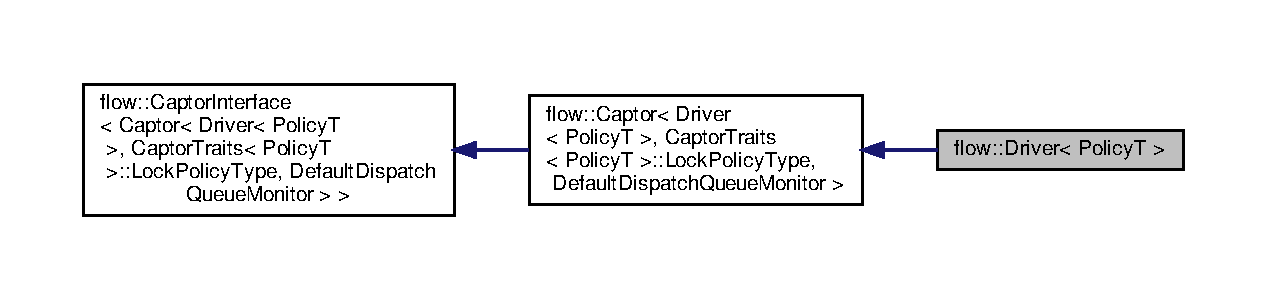
\includegraphics[width=350pt]{classflow_1_1_driver__inherit__graph}
\end{center}
\end{figure}


Collaboration diagram for flow\+:\+:Driver$<$ PolicyT $>$\+:
\nopagebreak
\begin{figure}[H]
\begin{center}
\leavevmode
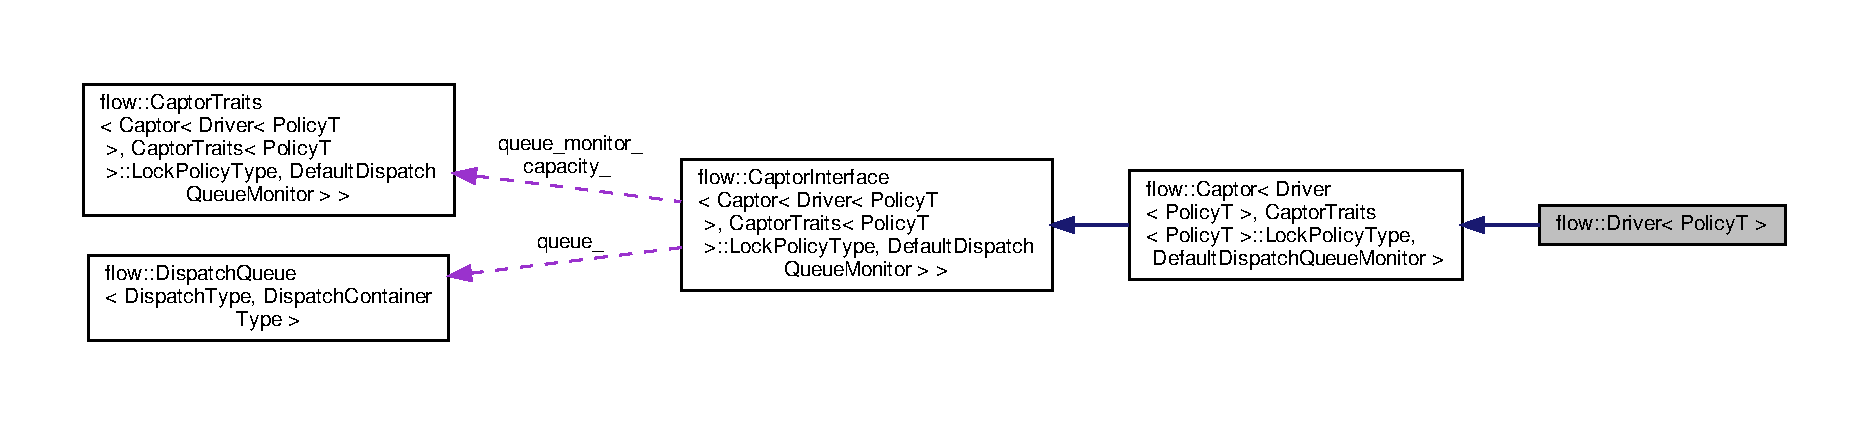
\includegraphics[width=350pt]{classflow_1_1_driver__coll__graph}
\end{center}
\end{figure}
\subsection*{Public Types}
\begin{DoxyCompactItemize}
\item 
\mbox{\Hypertarget{classflow_1_1_driver_a422446d9a2d8ae99613e3c5728956921}\label{classflow_1_1_driver_a422446d9a2d8ae99613e3c5728956921}} 
using \hyperlink{classflow_1_1_driver_a422446d9a2d8ae99613e3c5728956921}{Dispatch\+Container\+Type} = typename \hyperlink{structflow_1_1_captor_traits}{Captor\+Traits}$<$ PolicyT $>$\+::\hyperlink{classflow_1_1_driver_a422446d9a2d8ae99613e3c5728956921}{Dispatch\+Container\+Type}
\begin{DoxyCompactList}\small\item\em Underlying dispatch container type. \end{DoxyCompactList}\item 
\mbox{\Hypertarget{classflow_1_1_driver_ab20e67754359b2e562ef594672ee8855}\label{classflow_1_1_driver_ab20e67754359b2e562ef594672ee8855}} 
using \hyperlink{classflow_1_1_driver_ab20e67754359b2e562ef594672ee8855}{Dispatch\+Queue\+Monitor\+Type} = typename \hyperlink{structflow_1_1_captor_traits}{Captor\+Traits}$<$ PolicyT $>$\+::\hyperlink{classflow_1_1_driver_ab20e67754359b2e562ef594672ee8855}{Dispatch\+Queue\+Monitor\+Type}
\begin{DoxyCompactList}\small\item\em Queue monitor type. \end{DoxyCompactList}\item 
\mbox{\Hypertarget{classflow_1_1_driver_a29830caddd19fac6828c5f3eb8df5e65}\label{classflow_1_1_driver_a29830caddd19fac6828c5f3eb8df5e65}} 
using \hyperlink{classflow_1_1_driver_a29830caddd19fac6828c5f3eb8df5e65}{stamp\+\_\+type} = typename \hyperlink{structflow_1_1_captor_traits}{Captor\+Traits}$<$ PolicyT $>$\+::\hyperlink{classflow_1_1_driver_a29830caddd19fac6828c5f3eb8df5e65}{stamp\+\_\+type}
\begin{DoxyCompactList}\small\item\em Data stamp type. \end{DoxyCompactList}\end{DoxyCompactItemize}
\subsection*{Public Member Functions}
\begin{DoxyCompactItemize}
\item 
\hyperlink{classflow_1_1_driver_a195110b2344944c9154290e3aa0e6684}{Driver} (const \hyperlink{classflow_1_1_driver_a422446d9a2d8ae99613e3c5728956921}{Dispatch\+Container\+Type} \&container, const \hyperlink{classflow_1_1_driver_ab20e67754359b2e562ef594672ee8855}{Dispatch\+Queue\+Monitor\+Type} \&queue\+\_\+monitor)
\begin{DoxyCompactList}\small\item\em \hyperlink{classflow_1_1_dispatch}{Dispatch} container constructor. \end{DoxyCompactList}\end{DoxyCompactItemize}
\subsection*{Additional Inherited Members}


\subsection{Detailed Description}
\subsubsection*{template$<$typename PolicyT$>$\newline
class flow\+::\+Driver$<$ Policy\+T $>$}

C\+R\+T\+P-\/base for \hyperlink{classflow_1_1_driver}{Driver} input-\/capture policies. 

Captures data produces a synchronization sequencing range used to synchronize data produced by \hyperlink{classflow_1_1_follower}{Follower} buffers


\begin{DoxyTemplParams}{Template Parameters}
{\em PolicyT} & C\+R\+T\+P-\/derived captor with specialized capture policy \\
\hline
\end{DoxyTemplParams}


\subsection{Constructor \& Destructor Documentation}
\mbox{\Hypertarget{classflow_1_1_driver_a195110b2344944c9154290e3aa0e6684}\label{classflow_1_1_driver_a195110b2344944c9154290e3aa0e6684}} 
\index{flow\+::\+Driver@{flow\+::\+Driver}!Driver@{Driver}}
\index{Driver@{Driver}!flow\+::\+Driver@{flow\+::\+Driver}}
\subsubsection{\texorpdfstring{Driver()}{Driver()}}
{\footnotesize\ttfamily template$<$typename PolicyT$>$ \\
\hyperlink{classflow_1_1_driver}{flow\+::\+Driver}$<$ PolicyT $>$\+::\hyperlink{classflow_1_1_driver}{Driver} (\begin{DoxyParamCaption}\item[{const \hyperlink{classflow_1_1_driver_a422446d9a2d8ae99613e3c5728956921}{Dispatch\+Container\+Type} \&}]{container,  }\item[{const \hyperlink{classflow_1_1_driver_ab20e67754359b2e562ef594672ee8855}{Dispatch\+Queue\+Monitor\+Type} \&}]{queue\+\_\+monitor }\end{DoxyParamCaption})\hspace{0.3cm}{\ttfamily [explicit]}}



\hyperlink{classflow_1_1_dispatch}{Dispatch} container constructor. 


\begin{DoxyParams}{Parameters}
{\em container} & container object with some initial state \\
\hline
{\em queue\+\_\+monitor} & queue monitor with some initial state \\
\hline
\end{DoxyParams}


The documentation for this class was generated from the following file\+:\begin{DoxyCompactItemize}
\item 
flow/include/driver/\hyperlink{driver_8h}{driver.\+h}\end{DoxyCompactItemize}

\hypertarget{classflow_1_1_follower}{}\section{flow\+:\+:Follower$<$ PolicyT $>$ Class Template Reference}
\label{classflow_1_1_follower}\index{flow\+::\+Follower$<$ Policy\+T $>$@{flow\+::\+Follower$<$ Policy\+T $>$}}


C\+R\+T\+P-\/base for \hyperlink{classflow_1_1_follower}{Follower} input-\/capture policies.  




{\ttfamily \#include $<$follower.\+h$>$}



Inheritance diagram for flow\+:\+:Follower$<$ PolicyT $>$\+:
\nopagebreak
\begin{figure}[H]
\begin{center}
\leavevmode
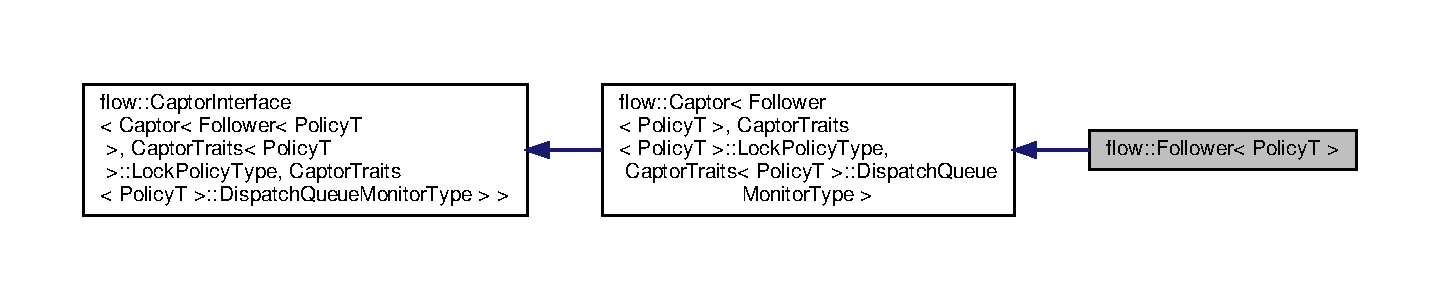
\includegraphics[width=350pt]{classflow_1_1_follower__inherit__graph}
\end{center}
\end{figure}


Collaboration diagram for flow\+:\+:Follower$<$ PolicyT $>$\+:
\nopagebreak
\begin{figure}[H]
\begin{center}
\leavevmode
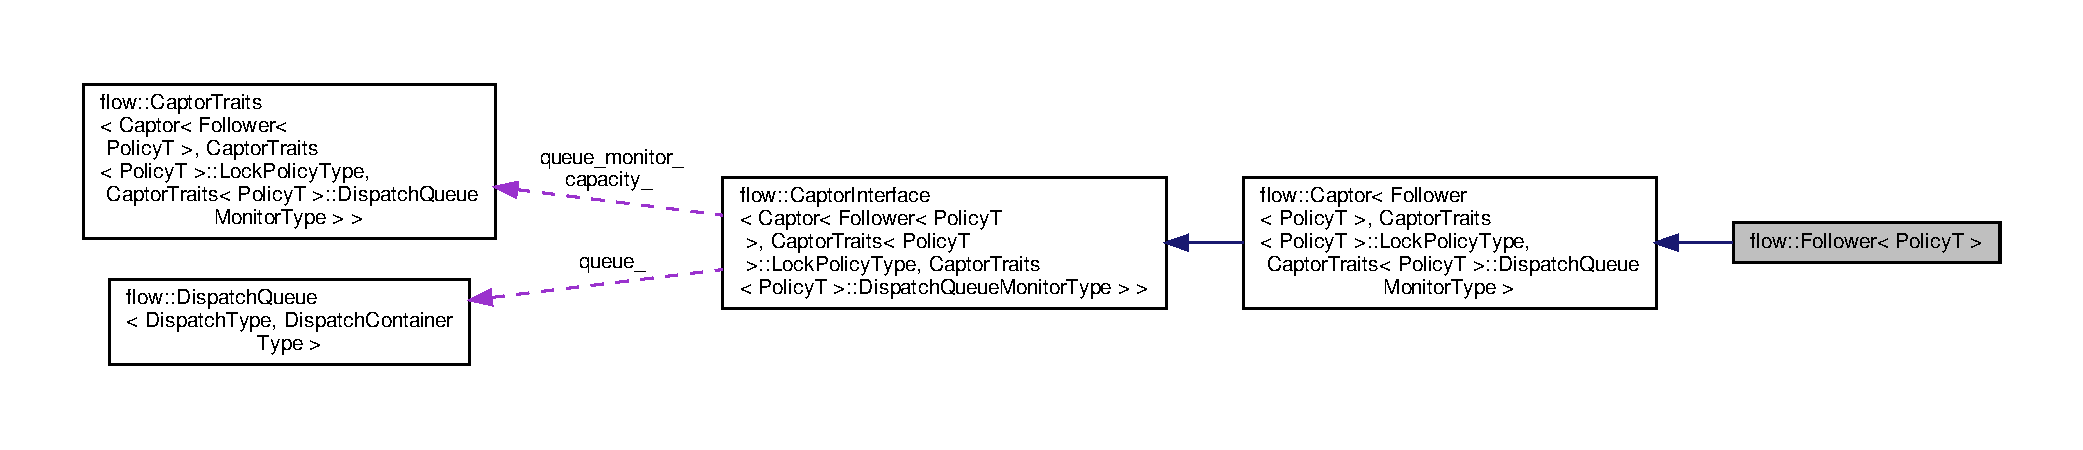
\includegraphics[width=350pt]{classflow_1_1_follower__coll__graph}
\end{center}
\end{figure}
\subsection*{Public Types}
\begin{DoxyCompactItemize}
\item 
\mbox{\Hypertarget{classflow_1_1_follower_a2c30490de514f45d9cc287eb8baed5db}\label{classflow_1_1_follower_a2c30490de514f45d9cc287eb8baed5db}} 
using \hyperlink{classflow_1_1_follower_a2c30490de514f45d9cc287eb8baed5db}{Dispatch\+Container\+Type} = typename \hyperlink{structflow_1_1_captor_traits}{Captor\+Traits}$<$ PolicyT $>$\+::\hyperlink{classflow_1_1_follower_a2c30490de514f45d9cc287eb8baed5db}{Dispatch\+Container\+Type}
\begin{DoxyCompactList}\small\item\em Underlying dispatch container type. \end{DoxyCompactList}\item 
\mbox{\Hypertarget{classflow_1_1_follower_aa19997fc64e57b6603f167144927de45}\label{classflow_1_1_follower_aa19997fc64e57b6603f167144927de45}} 
using \hyperlink{classflow_1_1_follower_aa19997fc64e57b6603f167144927de45}{Dispatch\+Queue\+Monitor\+Type} = typename \hyperlink{structflow_1_1_captor_traits}{Captor\+Traits}$<$ PolicyT $>$\+::\hyperlink{classflow_1_1_follower_aa19997fc64e57b6603f167144927de45}{Dispatch\+Queue\+Monitor\+Type}
\begin{DoxyCompactList}\small\item\em Queue monitor/capture preconditioning type. \end{DoxyCompactList}\item 
\mbox{\Hypertarget{classflow_1_1_follower_a1388657aef71e23dd17a18ed7c628ae0}\label{classflow_1_1_follower_a1388657aef71e23dd17a18ed7c628ae0}} 
using \hyperlink{classflow_1_1_follower_a1388657aef71e23dd17a18ed7c628ae0}{stamp\+\_\+type} = typename \hyperlink{structflow_1_1_captor_traits}{Captor\+Traits}$<$ PolicyT $>$\+::\hyperlink{classflow_1_1_follower_a1388657aef71e23dd17a18ed7c628ae0}{stamp\+\_\+type}
\begin{DoxyCompactList}\small\item\em Data stamp type. \end{DoxyCompactList}\end{DoxyCompactItemize}
\subsection*{Public Member Functions}
\begin{DoxyCompactItemize}
\item 
\hyperlink{classflow_1_1_follower_a3355c5acbcb1daea2fbe8e0c39f7b558}{Follower} (const \hyperlink{classflow_1_1_follower_a2c30490de514f45d9cc287eb8baed5db}{Dispatch\+Container\+Type} \&container, const \hyperlink{classflow_1_1_follower_aa19997fc64e57b6603f167144927de45}{Dispatch\+Queue\+Monitor\+Type} \&queue\+\_\+monitor)
\begin{DoxyCompactList}\small\item\em Initialization constructor. \end{DoxyCompactList}\end{DoxyCompactItemize}
\subsection*{Additional Inherited Members}


\subsection{Detailed Description}
\subsubsection*{template$<$typename PolicyT$>$\newline
class flow\+::\+Follower$<$ Policy\+T $>$}

C\+R\+T\+P-\/base for \hyperlink{classflow_1_1_follower}{Follower} input-\/capture policies. 

Captures data w.\+r.\+t to a driving sequencing range, produced by a \hyperlink{classflow_1_1_driver}{Driver}, according to a synchronization policy


\begin{DoxyTemplParams}{Template Parameters}
{\em PolicyT} & C\+R\+T\+P-\/derived captor with specialized capture policy \\
\hline
\end{DoxyTemplParams}


\subsection{Constructor \& Destructor Documentation}
\mbox{\Hypertarget{classflow_1_1_follower_a3355c5acbcb1daea2fbe8e0c39f7b558}\label{classflow_1_1_follower_a3355c5acbcb1daea2fbe8e0c39f7b558}} 
\index{flow\+::\+Follower@{flow\+::\+Follower}!Follower@{Follower}}
\index{Follower@{Follower}!flow\+::\+Follower@{flow\+::\+Follower}}
\subsubsection{\texorpdfstring{Follower()}{Follower()}}
{\footnotesize\ttfamily template$<$typename PolicyT$>$ \\
\hyperlink{classflow_1_1_follower}{flow\+::\+Follower}$<$ PolicyT $>$\+::\hyperlink{classflow_1_1_follower}{Follower} (\begin{DoxyParamCaption}\item[{const \hyperlink{classflow_1_1_follower_a2c30490de514f45d9cc287eb8baed5db}{Dispatch\+Container\+Type} \&}]{container,  }\item[{const \hyperlink{classflow_1_1_follower_aa19997fc64e57b6603f167144927de45}{Dispatch\+Queue\+Monitor\+Type} \&}]{queue\+\_\+monitor }\end{DoxyParamCaption})}



Initialization constructor. 


\begin{DoxyParams}{Parameters}
{\em container} & container object with some initial state \\
\hline
{\em queue\+\_\+monitor} & queue monitor with some initial state \\
\hline
\end{DoxyParams}


The documentation for this class was generated from the following file\+:\begin{DoxyCompactItemize}
\item 
flow/include/follower/\hyperlink{follower_8h}{follower.\+h}\end{DoxyCompactItemize}

\hypertarget{structflow_1_1is__capture__range}{}\section{flow\+:\+:is\+\_\+capture\+\_\+range$<$ RangeT $>$ Struct Template Reference}
\label{structflow_1_1is__capture__range}\index{flow\+::is\+\_\+capture\+\_\+range$<$ Range\+T $>$@{flow\+::is\+\_\+capture\+\_\+range$<$ Range\+T $>$}}


Checks if object type is an instance of \hyperlink{structflow_1_1_capture_range}{Capture\+Range}.  




{\ttfamily \#include $<$dispatch.\+h$>$}



Inheritance diagram for flow\+:\+:is\+\_\+capture\+\_\+range$<$ RangeT $>$\+:
\nopagebreak
\begin{figure}[H]
\begin{center}
\leavevmode
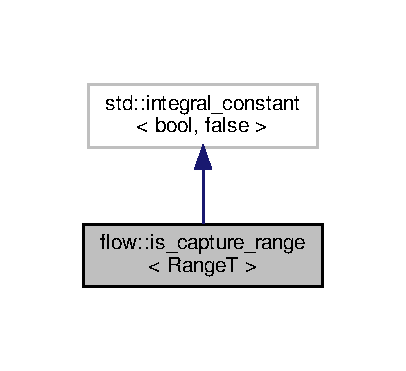
\includegraphics[width=195pt]{structflow_1_1is__capture__range__inherit__graph}
\end{center}
\end{figure}


Collaboration diagram for flow\+:\+:is\+\_\+capture\+\_\+range$<$ RangeT $>$\+:
\nopagebreak
\begin{figure}[H]
\begin{center}
\leavevmode
\includegraphics[width=195pt]{structflow_1_1is__capture__range__coll__graph}
\end{center}
\end{figure}


\subsection{Detailed Description}
\subsubsection*{template$<$typename RangeT$>$\newline
struct flow\+::is\+\_\+capture\+\_\+range$<$ Range\+T $>$}

Checks if object type is an instance of \hyperlink{structflow_1_1_capture_range}{Capture\+Range}. 


\begin{DoxyParams}{Parameters}
{\em RangeT} & object type to test \\
\hline
\end{DoxyParams}


The documentation for this struct was generated from the following file\+:\begin{DoxyCompactItemize}
\item 
flow/include/\hyperlink{dispatch_8h}{dispatch.\+h}\end{DoxyCompactItemize}

\hypertarget{structflow_1_1is__capture__range_3_01_capture_range_3_01_stamp_t_01_4_01_4}{}\section{flow\+:\+:is\+\_\+capture\+\_\+range$<$ Capture\+Range$<$ StampT $>$ $>$ Struct Template Reference}
\label{structflow_1_1is__capture__range_3_01_capture_range_3_01_stamp_t_01_4_01_4}\index{flow\+::is\+\_\+capture\+\_\+range$<$ Capture\+Range$<$ Stamp\+T $>$ $>$@{flow\+::is\+\_\+capture\+\_\+range$<$ Capture\+Range$<$ Stamp\+T $>$ $>$}}


Checks if object type is an instance of \hyperlink{structflow_1_1_capture_range}{Capture\+Range}.  




{\ttfamily \#include $<$dispatch.\+h$>$}



Inheritance diagram for flow\+:\+:is\+\_\+capture\+\_\+range$<$ Capture\+Range$<$ StampT $>$ $>$\+:
\nopagebreak
\begin{figure}[H]
\begin{center}
\leavevmode
\includegraphics[width=230pt]{structflow_1_1is__capture__range_3_01_capture_range_3_01_stamp_t_01_4_01_4__inherit__graph}
\end{center}
\end{figure}


Collaboration diagram for flow\+:\+:is\+\_\+capture\+\_\+range$<$ Capture\+Range$<$ StampT $>$ $>$\+:
\nopagebreak
\begin{figure}[H]
\begin{center}
\leavevmode
\includegraphics[width=230pt]{structflow_1_1is__capture__range_3_01_capture_range_3_01_stamp_t_01_4_01_4__coll__graph}
\end{center}
\end{figure}


\subsection{Detailed Description}
\subsubsection*{template$<$typename StampT$>$\newline
struct flow\+::is\+\_\+capture\+\_\+range$<$ Capture\+Range$<$ Stamp\+T $>$ $>$}

Checks if object type is an instance of \hyperlink{structflow_1_1_capture_range}{Capture\+Range}. 


\begin{DoxyParams}{Parameters}
{\em RangeT} & object type to test \\
\hline
\end{DoxyParams}


The documentation for this struct was generated from the following file\+:\begin{DoxyCompactItemize}
\item 
flow/include/\hyperlink{dispatch_8h}{dispatch.\+h}\end{DoxyCompactItemize}

\hypertarget{structflow_1_1is__driver}{}\section{flow\+:\+:is\+\_\+driver$<$ CaptorT $>$ Struct Template Reference}
\label{structflow_1_1is__driver}\index{flow\+::is\+\_\+driver$<$ Captor\+T $>$@{flow\+::is\+\_\+driver$<$ Captor\+T $>$}}


Checks if captor object derived from a \hyperlink{classflow_1_1_driver}{Driver} base.  




{\ttfamily \#include $<$captor.\+h$>$}



Inheritance diagram for flow\+:\+:is\+\_\+driver$<$ CaptorT $>$\+:\nopagebreak
\begin{figure}[H]
\begin{center}
\leavevmode
\includegraphics[width=350pt]{structflow_1_1is__driver__inherit__graph}
\end{center}
\end{figure}


Collaboration diagram for flow\+:\+:is\+\_\+driver$<$ CaptorT $>$\+:\nopagebreak
\begin{figure}[H]
\begin{center}
\leavevmode
\includegraphics[width=350pt]{structflow_1_1is__driver__coll__graph}
\end{center}
\end{figure}


\subsection{Detailed Description}
\subsubsection*{template$<$typename CaptorT$>$\newline
struct flow\+::is\+\_\+driver$<$ Captor\+T $>$}

Checks if captor object derived from a \hyperlink{classflow_1_1_driver}{Driver} base. 


\begin{DoxyTemplParams}{Template Parameters}
{\em CaptorT} & object to test\\
\hline
\end{DoxyTemplParams}

\begin{DoxyParams}{Parameters}
{\em CaptorT} & object to test \\
\hline
\end{DoxyParams}


The documentation for this struct was generated from the following file\+:\begin{DoxyCompactItemize}
\item 
flow/include/\hyperlink{captor_8h}{captor.\+h}\end{DoxyCompactItemize}

\hypertarget{structflow_1_1is__follower}{}\section{flow\+:\+:is\+\_\+follower$<$ CaptorT $>$ Struct Template Reference}
\label{structflow_1_1is__follower}\index{flow\+::is\+\_\+follower$<$ Captor\+T $>$@{flow\+::is\+\_\+follower$<$ Captor\+T $>$}}


Checks if captor object derived from a \hyperlink{classflow_1_1_follower}{Follower} base.  




{\ttfamily \#include $<$captor.\+h$>$}



Inheritance diagram for flow\+:\+:is\+\_\+follower$<$ CaptorT $>$\+:\nopagebreak
\begin{figure}[H]
\begin{center}
\leavevmode
\includegraphics[width=350pt]{structflow_1_1is__follower__inherit__graph}
\end{center}
\end{figure}


Collaboration diagram for flow\+:\+:is\+\_\+follower$<$ CaptorT $>$\+:\nopagebreak
\begin{figure}[H]
\begin{center}
\leavevmode
\includegraphics[width=350pt]{structflow_1_1is__follower__coll__graph}
\end{center}
\end{figure}


\subsection{Detailed Description}
\subsubsection*{template$<$typename CaptorT$>$\newline
struct flow\+::is\+\_\+follower$<$ Captor\+T $>$}

Checks if captor object derived from a \hyperlink{classflow_1_1_follower}{Follower} base. 


\begin{DoxyTemplParams}{Template Parameters}
{\em CaptorT} & object to test\\
\hline
\end{DoxyTemplParams}

\begin{DoxyParams}{Parameters}
{\em CaptorT} & object to test \\
\hline
\end{DoxyParams}


The documentation for this struct was generated from the following file\+:\begin{DoxyCompactItemize}
\item 
flow/include/\hyperlink{captor_8h}{captor.\+h}\end{DoxyCompactItemize}

\hypertarget{structflow_1_1is__no__lock}{}\section{flow\+:\+:is\+\_\+no\+\_\+lock$<$ LockableT $>$ Struct Template Reference}
\label{structflow_1_1is__no__lock}\index{flow\+::is\+\_\+no\+\_\+lock$<$ Lockable\+T $>$@{flow\+::is\+\_\+no\+\_\+lock$<$ Lockable\+T $>$}}


Checks if {\ttfamily LockableT} is of type \hyperlink{structflow_1_1_no_lock}{No\+Lock}.  




{\ttfamily \#include $<$captor.\+h$>$}



Inheritance diagram for flow\+:\+:is\+\_\+no\+\_\+lock$<$ LockableT $>$\+:\nopagebreak
\begin{figure}[H]
\begin{center}
\leavevmode
\includegraphics[width=232pt]{structflow_1_1is__no__lock__inherit__graph}
\end{center}
\end{figure}


Collaboration diagram for flow\+:\+:is\+\_\+no\+\_\+lock$<$ LockableT $>$\+:\nopagebreak
\begin{figure}[H]
\begin{center}
\leavevmode
\includegraphics[width=232pt]{structflow_1_1is__no__lock__coll__graph}
\end{center}
\end{figure}


\subsection{Detailed Description}
\subsubsection*{template$<$typename LockableT$>$\newline
struct flow\+::is\+\_\+no\+\_\+lock$<$ Lockable\+T $>$}

Checks if {\ttfamily LockableT} is of type \hyperlink{structflow_1_1_no_lock}{No\+Lock}. 


\begin{DoxyTemplParams}{Template Parameters}
{\em CaptorT} & object to test \\
\hline
\end{DoxyTemplParams}


The documentation for this struct was generated from the following file\+:\begin{DoxyCompactItemize}
\item 
flow/include/\hyperlink{captor_8h}{captor.\+h}\end{DoxyCompactItemize}

\hypertarget{structflow_1_1is__polling}{}\section{flow\+:\+:is\+\_\+polling$<$ CaptorT $>$ Struct Template Reference}
\label{structflow_1_1is__polling}\index{flow\+::is\+\_\+polling$<$ Captor\+T $>$@{flow\+::is\+\_\+polling$<$ Captor\+T $>$}}


Checks if captor is serviced by polling capture.  




{\ttfamily \#include $<$captor.\+h$>$}



Inheritance diagram for flow\+:\+:is\+\_\+polling$<$ CaptorT $>$\+:\nopagebreak
\begin{figure}[H]
\begin{center}
\leavevmode
\includegraphics[width=350pt]{structflow_1_1is__polling__inherit__graph}
\end{center}
\end{figure}


Collaboration diagram for flow\+:\+:is\+\_\+polling$<$ CaptorT $>$\+:\nopagebreak
\begin{figure}[H]
\begin{center}
\leavevmode
\includegraphics[width=350pt]{structflow_1_1is__polling__coll__graph}
\end{center}
\end{figure}


\subsection{Detailed Description}
\subsubsection*{template$<$typename CaptorT$>$\newline
struct flow\+::is\+\_\+polling$<$ Captor\+T $>$}

Checks if captor is serviced by polling capture. 


\begin{DoxyTemplParams}{Template Parameters}
{\em CaptorT} & object to test \\
\hline
\end{DoxyTemplParams}


The documentation for this struct was generated from the following file\+:\begin{DoxyCompactItemize}
\item 
flow/include/\hyperlink{captor_8h}{captor.\+h}\end{DoxyCompactItemize}

\hypertarget{structflow_1_1is__polling__lock}{}\section{flow\+:\+:is\+\_\+polling\+\_\+lock$<$ LockableT $>$ Struct Template Reference}
\label{structflow_1_1is__polling__lock}\index{flow\+::is\+\_\+polling\+\_\+lock$<$ Lockable\+T $>$@{flow\+::is\+\_\+polling\+\_\+lock$<$ Lockable\+T $>$}}


Checks if {\ttfamily LockableT} is instance of \hyperlink{structflow_1_1_polling_lock}{Polling\+Lock}.  




{\ttfamily \#include $<$captor.\+h$>$}



Inheritance diagram for flow\+:\+:is\+\_\+polling\+\_\+lock$<$ LockableT $>$\+:\nopagebreak
\begin{figure}[H]
\begin{center}
\leavevmode
\includegraphics[width=190pt]{structflow_1_1is__polling__lock__inherit__graph}
\end{center}
\end{figure}


Collaboration diagram for flow\+:\+:is\+\_\+polling\+\_\+lock$<$ LockableT $>$\+:\nopagebreak
\begin{figure}[H]
\begin{center}
\leavevmode
\includegraphics[width=190pt]{structflow_1_1is__polling__lock__coll__graph}
\end{center}
\end{figure}


\subsection{Detailed Description}
\subsubsection*{template$<$typename LockableT$>$\newline
struct flow\+::is\+\_\+polling\+\_\+lock$<$ Lockable\+T $>$}

Checks if {\ttfamily LockableT} is instance of \hyperlink{structflow_1_1_polling_lock}{Polling\+Lock}. 


\begin{DoxyTemplParams}{Template Parameters}
{\em CaptorT} & object to test \\
\hline
\end{DoxyTemplParams}


The documentation for this struct was generated from the following file\+:\begin{DoxyCompactItemize}
\item 
flow/include/\hyperlink{captor_8h}{captor.\+h}\end{DoxyCompactItemize}

\hypertarget{structflow_1_1is__polling__lock_3_01_polling_lock_3_01_lockable_t_01_4_01_4}{}\section{flow\+:\+:is\+\_\+polling\+\_\+lock$<$ Polling\+Lock$<$ LockableT $>$ $>$ Struct Template Reference}
\label{structflow_1_1is__polling__lock_3_01_polling_lock_3_01_lockable_t_01_4_01_4}\index{flow\+::is\+\_\+polling\+\_\+lock$<$ Polling\+Lock$<$ Lockable\+T $>$ $>$@{flow\+::is\+\_\+polling\+\_\+lock$<$ Polling\+Lock$<$ Lockable\+T $>$ $>$}}


Checks if {\ttfamily LockableT} is instance of \hyperlink{structflow_1_1_polling_lock}{Polling\+Lock}.  




{\ttfamily \#include $<$captor.\+h$>$}



Inheritance diagram for flow\+:\+:is\+\_\+polling\+\_\+lock$<$ Polling\+Lock$<$ LockableT $>$ $>$\+:\nopagebreak
\begin{figure}[H]
\begin{center}
\leavevmode
\includegraphics[width=228pt]{structflow_1_1is__polling__lock_3_01_polling_lock_3_01_lockable_t_01_4_01_4__inherit__graph}
\end{center}
\end{figure}


Collaboration diagram for flow\+:\+:is\+\_\+polling\+\_\+lock$<$ Polling\+Lock$<$ LockableT $>$ $>$\+:\nopagebreak
\begin{figure}[H]
\begin{center}
\leavevmode
\includegraphics[width=228pt]{structflow_1_1is__polling__lock_3_01_polling_lock_3_01_lockable_t_01_4_01_4__coll__graph}
\end{center}
\end{figure}


\subsection{Detailed Description}
\subsubsection*{template$<$typename LockableT$>$\newline
struct flow\+::is\+\_\+polling\+\_\+lock$<$ Polling\+Lock$<$ Lockable\+T $>$ $>$}

Checks if {\ttfamily LockableT} is instance of \hyperlink{structflow_1_1_polling_lock}{Polling\+Lock}. 


\begin{DoxyTemplParams}{Template Parameters}
{\em CaptorT} & object to test \\
\hline
\end{DoxyTemplParams}


The documentation for this struct was generated from the following file\+:\begin{DoxyCompactItemize}
\item 
flow/include/\hyperlink{captor_8h}{captor.\+h}\end{DoxyCompactItemize}

\hypertarget{classflow_1_1follower_1_1_latched}{}\section{flow\+:\+:follower\+:\+:Latched$<$ DispatchT, Lock\+PolicyT, ContainerT, Queue\+MonitorT $>$ Class Template Reference}
\label{classflow_1_1follower_1_1_latched}\index{flow\+::follower\+::\+Latched$<$ Dispatch\+T, Lock\+Policy\+T, Container\+T, Queue\+Monitor\+T $>$@{flow\+::follower\+::\+Latched$<$ Dispatch\+T, Lock\+Policy\+T, Container\+T, Queue\+Monitor\+T $>$}}


Captures one element before the capture range lower bound, minus a minimum period.  




{\ttfamily \#include $<$latched.\+h$>$}



Inheritance diagram for flow\+:\+:follower\+:\+:Latched$<$ DispatchT, Lock\+PolicyT, ContainerT, Queue\+MonitorT $>$\+:
\nopagebreak
\begin{figure}[H]
\begin{center}
\leavevmode
\includegraphics[width=350pt]{classflow_1_1follower_1_1_latched__inherit__graph}
\end{center}
\end{figure}


Collaboration diagram for flow\+:\+:follower\+:\+:Latched$<$ DispatchT, Lock\+PolicyT, ContainerT, Queue\+MonitorT $>$\+:
\nopagebreak
\begin{figure}[H]
\begin{center}
\leavevmode
\includegraphics[width=350pt]{classflow_1_1follower_1_1_latched__coll__graph}
\end{center}
\end{figure}
\subsection*{Public Types}
\begin{DoxyCompactItemize}
\item 
\mbox{\Hypertarget{classflow_1_1follower_1_1_latched_a330b7f9dd745cd2b513b21789250131d}\label{classflow_1_1follower_1_1_latched_a330b7f9dd745cd2b513b21789250131d}} 
using \hyperlink{classflow_1_1follower_1_1_latched_a330b7f9dd745cd2b513b21789250131d}{stamp\+\_\+type} = typename \hyperlink{structflow_1_1_captor_traits}{Captor\+Traits}$<$ \hyperlink{classflow_1_1follower_1_1_latched}{Latched} $>$\+::\hyperlink{classflow_1_1follower_1_1_latched_a330b7f9dd745cd2b513b21789250131d}{stamp\+\_\+type}
\begin{DoxyCompactList}\small\item\em Data stamp type. \end{DoxyCompactList}\item 
\mbox{\Hypertarget{classflow_1_1follower_1_1_latched_a437fa0b63a9d5c36c7a63774a53d6552}\label{classflow_1_1follower_1_1_latched_a437fa0b63a9d5c36c7a63774a53d6552}} 
using \hyperlink{classflow_1_1follower_1_1_latched_a437fa0b63a9d5c36c7a63774a53d6552}{offset\+\_\+type} = typename \hyperlink{structflow_1_1_captor_traits}{Captor\+Traits}$<$ \hyperlink{classflow_1_1follower_1_1_latched}{Latched} $>$\+::\hyperlink{classflow_1_1follower_1_1_latched_a437fa0b63a9d5c36c7a63774a53d6552}{offset\+\_\+type}
\begin{DoxyCompactList}\small\item\em Data stamp duration type. \end{DoxyCompactList}\end{DoxyCompactItemize}
\subsection*{Public Member Functions}
\begin{DoxyCompactItemize}
\item 
\hyperlink{classflow_1_1follower_1_1_latched_a5974d2c9a24b8ef6d9e1f71b696fafdb}{Latched} (const \hyperlink{classflow_1_1follower_1_1_latched_a437fa0b63a9d5c36c7a63774a53d6552}{offset\+\_\+type} min\+\_\+period, const ContainerT \&container=ContainerT\{\}, const Queue\+MonitorT \&queue\+\_\+monitor=Queue\+MonitorT\{\})
\begin{DoxyCompactList}\small\item\em Setup constructor. \end{DoxyCompactList}\end{DoxyCompactItemize}
\subsection*{Additional Inherited Members}


\subsection{Detailed Description}
\subsubsection*{template$<$typename DispatchT, typename Lock\+PolicyT = No\+Lock, typename ContainerT = Default\+Container$<$\+Dispatch\+T$>$, typename Queue\+MonitorT = Default\+Dispatch\+Queue\+Monitor$>$\newline
class flow\+::follower\+::\+Latched$<$ Dispatch\+T, Lock\+Policy\+T, Container\+T, Queue\+Monitor\+T $>$}

Captures one element before the capture range lower bound, minus a minimum period. 

All older elements are removed. If no newer elements are present on the next capture attempt, then the last captured element is returned. If a newer element is present on a subsequent capture attempt, meeting the aforementioned qualifications, this elements is captured and replaces \char`\"{}latched\char`\"{} element state.


\begin{DoxyTemplParams}{Template Parameters}
{\em DispatchT} & data dispatch type \\
\hline
{\em Lock\+PolicyT} & a Basic\+Lockable (\href{https://en.cppreference.com/w/cpp/named_req/BasicLockable}{\tt https\+://en.\+cppreference.\+com/w/cpp/named\+\_\+req/\+Basic\+Lockable}) object or \hyperlink{structflow_1_1_no_lock}{No\+Lock} or \hyperlink{structflow_1_1_polling_lock}{Polling\+Lock} \\
\hline
{\em ContainerT} & underlying {\ttfamily DispatchT} container type \\
\hline
{\em Queue\+MonitorT} & object used to monitor queue state on each insertion; used to precondition capture\\
\hline
\end{DoxyTemplParams}
\begin{DoxyNote}{Note}
\hyperlink{classflow_1_1follower_1_1_latched}{Latched} won\textquotesingle{}t behave non-\/deterministically if actual input period (difference between successive dispatch stamps) is greater than {\ttfamily min\+\_\+period}. However, newer data values will not be captured if they are within a {\ttfamily min\+\_\+period{\ttfamily  offset of {\ttfamily range.\+lower\+\_\+stamp}}}
\end{DoxyNote}
\hyperlink{classflow_1_1follower_1_1_latched}{Latched} may never enter a R\+E\+A\+DY state if data never becomes available. Calling application may need to implement a synchronization timeout behavior 

\subsection{Constructor \& Destructor Documentation}
\mbox{\Hypertarget{classflow_1_1follower_1_1_latched_a5974d2c9a24b8ef6d9e1f71b696fafdb}\label{classflow_1_1follower_1_1_latched_a5974d2c9a24b8ef6d9e1f71b696fafdb}} 
\index{flow\+::follower\+::\+Latched@{flow\+::follower\+::\+Latched}!Latched@{Latched}}
\index{Latched@{Latched}!flow\+::follower\+::\+Latched@{flow\+::follower\+::\+Latched}}
\subsubsection{\texorpdfstring{Latched()}{Latched()}}
{\footnotesize\ttfamily template$<$typename DispatchT , typename Lock\+PolicyT  = No\+Lock, typename ContainerT  = Default\+Container$<$\+Dispatch\+T$>$, typename Queue\+MonitorT  = Default\+Dispatch\+Queue\+Monitor$>$ \\
\hyperlink{classflow_1_1follower_1_1_latched}{flow\+::follower\+::\+Latched}$<$ DispatchT, Lock\+PolicyT, ContainerT, Queue\+MonitorT $>$\+::\hyperlink{classflow_1_1follower_1_1_latched}{Latched} (\begin{DoxyParamCaption}\item[{const \hyperlink{classflow_1_1follower_1_1_latched_a437fa0b63a9d5c36c7a63774a53d6552}{offset\+\_\+type}}]{min\+\_\+period,  }\item[{const ContainerT \&}]{container = {\ttfamily ContainerT\{\}},  }\item[{const Queue\+MonitorT \&}]{queue\+\_\+monitor = {\ttfamily QueueMonitorT\{\}} }\end{DoxyParamCaption})\hspace{0.3cm}{\ttfamily [explicit]}}



Setup constructor. 


\begin{DoxyParams}{Parameters}
{\em min\+\_\+period} & minimum expected difference between data stamps \\
\hline
{\em container} & container object with some initial state \\
\hline
{\em queue\+\_\+monitor} & queue monitor with some initial state\\
\hline
\end{DoxyParams}

\begin{DoxyExceptions}{Exceptions}
{\em $<$code$>$std\+::invalid\+\_\+argument$<$/code$>$} & if {\ttfamily m\+\_\+after $<$ 1} \\
\hline
\end{DoxyExceptions}


The documentation for this class was generated from the following file\+:\begin{DoxyCompactItemize}
\item 
flow/include/follower/\hyperlink{latched_8h}{latched.\+h}\end{DoxyCompactItemize}

\hypertarget{classflow_1_1follower_1_1_matched_stamp}{}\section{flow\+:\+:follower\+:\+:Matched\+Stamp$<$ DispatchT, Lock\+PolicyT, ContainerT, Queue\+MonitorT $>$ Class Template Reference}
\label{classflow_1_1follower_1_1_matched_stamp}\index{flow\+::follower\+::\+Matched\+Stamp$<$ Dispatch\+T, Lock\+Policy\+T, Container\+T, Queue\+Monitor\+T $>$@{flow\+::follower\+::\+Matched\+Stamp$<$ Dispatch\+T, Lock\+Policy\+T, Container\+T, Queue\+Monitor\+T $>$}}


Captures one element with a stamp which exactly matches the capture range lower bound.  




{\ttfamily \#include $<$matched\+\_\+stamp.\+h$>$}



Inheritance diagram for flow\+:\+:follower\+:\+:Matched\+Stamp$<$ DispatchT, Lock\+PolicyT, ContainerT, Queue\+MonitorT $>$\+:
\nopagebreak
\begin{figure}[H]
\begin{center}
\leavevmode
\includegraphics[width=350pt]{classflow_1_1follower_1_1_matched_stamp__inherit__graph}
\end{center}
\end{figure}


Collaboration diagram for flow\+:\+:follower\+:\+:Matched\+Stamp$<$ DispatchT, Lock\+PolicyT, ContainerT, Queue\+MonitorT $>$\+:
\nopagebreak
\begin{figure}[H]
\begin{center}
\leavevmode
\includegraphics[width=350pt]{classflow_1_1follower_1_1_matched_stamp__coll__graph}
\end{center}
\end{figure}
\subsection*{Public Types}
\begin{DoxyCompactItemize}
\item 
\mbox{\Hypertarget{classflow_1_1follower_1_1_matched_stamp_a46f9d99cd263a83d976d8f1bcb62bee0}\label{classflow_1_1follower_1_1_matched_stamp_a46f9d99cd263a83d976d8f1bcb62bee0}} 
using \hyperlink{classflow_1_1follower_1_1_matched_stamp_a46f9d99cd263a83d976d8f1bcb62bee0}{stamp\+\_\+type} = typename \hyperlink{structflow_1_1_captor_traits}{Captor\+Traits}$<$ \hyperlink{classflow_1_1follower_1_1_matched_stamp}{Matched\+Stamp} $>$\+::\hyperlink{classflow_1_1follower_1_1_matched_stamp_a46f9d99cd263a83d976d8f1bcb62bee0}{stamp\+\_\+type}
\begin{DoxyCompactList}\small\item\em Data stamp type. \end{DoxyCompactList}\end{DoxyCompactItemize}
\subsection*{Public Member Functions}
\begin{DoxyCompactItemize}
\item 
\hyperlink{classflow_1_1follower_1_1_matched_stamp_a67f6b9b316170b553333d3c25dd47be0}{Matched\+Stamp} (const ContainerT \&container=ContainerT\{\}, const Queue\+MonitorT \&queue\+\_\+monitor=Queue\+MonitorT\{\})
\begin{DoxyCompactList}\small\item\em Setup constructor. \end{DoxyCompactList}\end{DoxyCompactItemize}
\subsection*{Additional Inherited Members}


\subsection{Detailed Description}
\subsubsection*{template$<$typename DispatchT, typename Lock\+PolicyT = No\+Lock, typename ContainerT = Default\+Container$<$\+Dispatch\+T$>$, typename Queue\+MonitorT = Default\+Dispatch\+Queue\+Monitor$>$\newline
class flow\+::follower\+::\+Matched\+Stamp$<$ Dispatch\+T, Lock\+Policy\+T, Container\+T, Queue\+Monitor\+T $>$}

Captures one element with a stamp which exactly matches the capture range lower bound. 

All older elements are removed.


\begin{DoxyTemplParams}{Template Parameters}
{\em DispatchT} & data dispatch type \\
\hline
{\em Lock\+PolicyT} & a Basic\+Lockable (\href{https://en.cppreference.com/w/cpp/named_req/BasicLockable}{\tt https\+://en.\+cppreference.\+com/w/cpp/named\+\_\+req/\+Basic\+Lockable}) object or \hyperlink{structflow_1_1_no_lock}{No\+Lock} or \hyperlink{structflow_1_1_polling_lock}{Polling\+Lock} \\
\hline
{\em ContainerT} & underlying {\ttfamily DispatchT} container type \\
\hline
{\em Queue\+MonitorT} & object used to monitor queue state on each insertion; used to precondition capture \\
\hline
\end{DoxyTemplParams}


\subsection{Constructor \& Destructor Documentation}
\mbox{\Hypertarget{classflow_1_1follower_1_1_matched_stamp_a67f6b9b316170b553333d3c25dd47be0}\label{classflow_1_1follower_1_1_matched_stamp_a67f6b9b316170b553333d3c25dd47be0}} 
\index{flow\+::follower\+::\+Matched\+Stamp@{flow\+::follower\+::\+Matched\+Stamp}!Matched\+Stamp@{Matched\+Stamp}}
\index{Matched\+Stamp@{Matched\+Stamp}!flow\+::follower\+::\+Matched\+Stamp@{flow\+::follower\+::\+Matched\+Stamp}}
\subsubsection{\texorpdfstring{Matched\+Stamp()}{MatchedStamp()}}
{\footnotesize\ttfamily template$<$typename DispatchT , typename Lock\+PolicyT  = No\+Lock, typename ContainerT  = Default\+Container$<$\+Dispatch\+T$>$, typename Queue\+MonitorT  = Default\+Dispatch\+Queue\+Monitor$>$ \\
\hyperlink{classflow_1_1follower_1_1_matched_stamp}{flow\+::follower\+::\+Matched\+Stamp}$<$ DispatchT, Lock\+PolicyT, ContainerT, Queue\+MonitorT $>$\+::\hyperlink{classflow_1_1follower_1_1_matched_stamp}{Matched\+Stamp} (\begin{DoxyParamCaption}\item[{const ContainerT \&}]{container = {\ttfamily ContainerT\{\}},  }\item[{const Queue\+MonitorT \&}]{queue\+\_\+monitor = {\ttfamily QueueMonitorT\{\}} }\end{DoxyParamCaption})\hspace{0.3cm}{\ttfamily [explicit]}}



Setup constructor. 


\begin{DoxyParams}{Parameters}
{\em container} & container object with some initial state \\
\hline
{\em queue\+\_\+monitor} & queue monitor with some initial state \\
\hline
\end{DoxyParams}


The documentation for this class was generated from the following file\+:\begin{DoxyCompactItemize}
\item 
flow/include/follower/\hyperlink{matched__stamp_8h}{matched\+\_\+stamp.\+h}\end{DoxyCompactItemize}

\hypertarget{classflow_1_1driver_1_1_next}{}\section{flow\+:\+:driver\+:\+:Next$<$ DispatchT, Lock\+PolicyT, ContainerT, Queue\+MonitorT $>$ Class Template Reference}
\label{classflow_1_1driver_1_1_next}\index{flow\+::driver\+::\+Next$<$ Dispatch\+T, Lock\+Policy\+T, Container\+T, Queue\+Monitor\+T $>$@{flow\+::driver\+::\+Next$<$ Dispatch\+T, Lock\+Policy\+T, Container\+T, Queue\+Monitor\+T $>$}}


Captures the next oldest data element.  




{\ttfamily \#include $<$next.\+h$>$}



Inheritance diagram for flow\+:\+:driver\+:\+:Next$<$ DispatchT, Lock\+PolicyT, ContainerT, Queue\+MonitorT $>$\+:
\nopagebreak
\begin{figure}[H]
\begin{center}
\leavevmode
\includegraphics[width=350pt]{classflow_1_1driver_1_1_next__inherit__graph}
\end{center}
\end{figure}


Collaboration diagram for flow\+:\+:driver\+:\+:Next$<$ DispatchT, Lock\+PolicyT, ContainerT, Queue\+MonitorT $>$\+:
\nopagebreak
\begin{figure}[H]
\begin{center}
\leavevmode
\includegraphics[width=350pt]{classflow_1_1driver_1_1_next__coll__graph}
\end{center}
\end{figure}
\subsection*{Public Types}
\begin{DoxyCompactItemize}
\item 
\mbox{\Hypertarget{classflow_1_1driver_1_1_next_a642dfa5c658efdc32d41b90fb71ea3a6}\label{classflow_1_1driver_1_1_next_a642dfa5c658efdc32d41b90fb71ea3a6}} 
using \hyperlink{classflow_1_1driver_1_1_next_a642dfa5c658efdc32d41b90fb71ea3a6}{size\+\_\+type} = typename \hyperlink{structflow_1_1_captor_traits}{Captor\+Traits}$<$ \hyperlink{classflow_1_1driver_1_1_next}{Next} $>$\+::\hyperlink{classflow_1_1driver_1_1_next_a642dfa5c658efdc32d41b90fb71ea3a6}{size\+\_\+type}
\begin{DoxyCompactList}\small\item\em Integer size type. \end{DoxyCompactList}\item 
\mbox{\Hypertarget{classflow_1_1driver_1_1_next_ac011d6eebb7dd89de890c09295f98613}\label{classflow_1_1driver_1_1_next_ac011d6eebb7dd89de890c09295f98613}} 
using \hyperlink{classflow_1_1driver_1_1_next_ac011d6eebb7dd89de890c09295f98613}{stamp\+\_\+type} = typename \hyperlink{structflow_1_1_captor_traits}{Captor\+Traits}$<$ \hyperlink{classflow_1_1driver_1_1_next}{Next} $>$\+::\hyperlink{classflow_1_1driver_1_1_next_ac011d6eebb7dd89de890c09295f98613}{stamp\+\_\+type}
\begin{DoxyCompactList}\small\item\em Data stamp type. \end{DoxyCompactList}\end{DoxyCompactItemize}
\subsection*{Public Member Functions}
\begin{DoxyCompactItemize}
\item 
\hyperlink{classflow_1_1driver_1_1_next_a1313d1526a137be521b64bc9758a809e}{Next} (const ContainerT \&container=ContainerT\{\}, const Queue\+MonitorT \&queue\+\_\+monitor=Queue\+MonitorT\{\})
\begin{DoxyCompactList}\small\item\em Configuration constructor. \end{DoxyCompactList}\end{DoxyCompactItemize}
\subsection*{Additional Inherited Members}


\subsection{Detailed Description}
\subsubsection*{template$<$typename DispatchT, typename Lock\+PolicyT = No\+Lock, typename ContainerT = Default\+Container$<$\+Dispatch\+T$>$, typename Queue\+MonitorT = Default\+Dispatch\+Queue\+Monitor$>$\newline
class flow\+::driver\+::\+Next$<$ Dispatch\+T, Lock\+Policy\+T, Container\+T, Queue\+Monitor\+T $>$}

Captures the next oldest data element. 

Establishes a sequencing range with {\ttfamily range.\+lower\+\_\+stamp == range.\+upper\+\_\+stamp} equal to the captured element stamp. Removes captured element from buffer.


\begin{DoxyTemplParams}{Template Parameters}
{\em DispatchT} & data dispatch type \\
\hline
{\em Lock\+PolicyT} & a Basic\+Lockable (\href{https://en.cppreference.com/w/cpp/named_req/BasicLockable}{\tt https\+://en.\+cppreference.\+com/w/cpp/named\+\_\+req/\+Basic\+Lockable}) object or \hyperlink{structflow_1_1_no_lock}{No\+Lock} or \hyperlink{structflow_1_1_polling_lock}{Polling\+Lock} \\
\hline
{\em ContainerT} & underlying {\ttfamily DispatchT} container type \\
\hline
{\em Queue\+MonitorT} & object used to monitor queue state on each insertion \\
\hline
\end{DoxyTemplParams}


\subsection{Constructor \& Destructor Documentation}
\mbox{\Hypertarget{classflow_1_1driver_1_1_next_a1313d1526a137be521b64bc9758a809e}\label{classflow_1_1driver_1_1_next_a1313d1526a137be521b64bc9758a809e}} 
\index{flow\+::driver\+::\+Next@{flow\+::driver\+::\+Next}!Next@{Next}}
\index{Next@{Next}!flow\+::driver\+::\+Next@{flow\+::driver\+::\+Next}}
\subsubsection{\texorpdfstring{Next()}{Next()}}
{\footnotesize\ttfamily template$<$typename DispatchT , typename Lock\+PolicyT  = No\+Lock, typename ContainerT  = Default\+Container$<$\+Dispatch\+T$>$, typename Queue\+MonitorT  = Default\+Dispatch\+Queue\+Monitor$>$ \\
\hyperlink{classflow_1_1driver_1_1_next}{flow\+::driver\+::\+Next}$<$ DispatchT, Lock\+PolicyT, ContainerT, Queue\+MonitorT $>$\+::\hyperlink{classflow_1_1driver_1_1_next}{Next} (\begin{DoxyParamCaption}\item[{const ContainerT \&}]{container = {\ttfamily ContainerT\{\}},  }\item[{const Queue\+MonitorT \&}]{queue\+\_\+monitor = {\ttfamily QueueMonitorT\{\}} }\end{DoxyParamCaption})\hspace{0.3cm}{\ttfamily [explicit]}}



Configuration constructor. 


\begin{DoxyParams}{Parameters}
{\em container} & container object with some initial state \\
\hline
\end{DoxyParams}


The documentation for this class was generated from the following file\+:\begin{DoxyCompactItemize}
\item 
flow/include/driver/\hyperlink{next_8h}{next.\+h}\end{DoxyCompactItemize}

\hypertarget{structflow_1_1_no_capture}{}\section{flow\+:\+:No\+Capture Struct Reference}
\label{structflow_1_1_no_capture}\index{flow\+::\+No\+Capture@{flow\+::\+No\+Capture}}


Object used in place of output iterator as a placeholder with no data capture effects.  




{\ttfamily \#include $<$synchronizer.\+h$>$}

\subsection*{Public Member Functions}
\begin{DoxyCompactItemize}
\item 
\mbox{\Hypertarget{structflow_1_1_no_capture_a6cdb8878087a6cb0b03d4050de2bacd2}\label{structflow_1_1_no_capture_a6cdb8878087a6cb0b03d4050de2bacd2}} 
constexpr \hyperlink{structflow_1_1_no_capture}{No\+Capture} \& \hyperlink{structflow_1_1_no_capture_a6cdb8878087a6cb0b03d4050de2bacd2}{operator$\ast$} ()
\begin{DoxyCompactList}\small\item\em No-\/op. \end{DoxyCompactList}\item 
\mbox{\Hypertarget{structflow_1_1_no_capture_a8810966a2d47d6ecfce33f44a89452c6}\label{structflow_1_1_no_capture_a8810966a2d47d6ecfce33f44a89452c6}} 
constexpr \hyperlink{structflow_1_1_no_capture}{No\+Capture} \& \hyperlink{structflow_1_1_no_capture_a8810966a2d47d6ecfce33f44a89452c6}{operator++} ()
\begin{DoxyCompactList}\small\item\em No-\/op. \end{DoxyCompactList}\item 
\mbox{\Hypertarget{structflow_1_1_no_capture_aeee8bd120b81f470a1452dec50faa7eb}\label{structflow_1_1_no_capture_aeee8bd120b81f470a1452dec50faa7eb}} 
constexpr \hyperlink{structflow_1_1_no_capture}{No\+Capture} \& \hyperlink{structflow_1_1_no_capture_aeee8bd120b81f470a1452dec50faa7eb}{operator++} (int)
\begin{DoxyCompactList}\small\item\em No-\/op. \end{DoxyCompactList}\item 
\mbox{\Hypertarget{structflow_1_1_no_capture_a32b6d8820ee81727c3d076b9ab14bf6c}\label{structflow_1_1_no_capture_a32b6d8820ee81727c3d076b9ab14bf6c}} 
{\footnotesize template$<$typename ValueT $>$ }\\constexpr \hyperlink{structflow_1_1_no_capture}{No\+Capture} \& \hyperlink{structflow_1_1_no_capture_a32b6d8820ee81727c3d076b9ab14bf6c}{operator=} (ValueT \&\&)
\begin{DoxyCompactList}\small\item\em No-\/op. \end{DoxyCompactList}\end{DoxyCompactItemize}


\subsection{Detailed Description}
Object used in place of output iterator as a placeholder with no data capture effects. 

The documentation for this struct was generated from the following file\+:\begin{DoxyCompactItemize}
\item 
flow/include/\hyperlink{synchronizer_8h}{synchronizer.\+h}\end{DoxyCompactItemize}

\hypertarget{structflow_1_1_no_lock}{}\section{flow\+:\+:No\+Lock Struct Reference}
\label{structflow_1_1_no_lock}\index{flow\+::\+No\+Lock@{flow\+::\+No\+Lock}}


Stand-\/in type used to signify that captors will be used in a single-\/threaded context.  




{\ttfamily \#include $<$captor.\+h$>$}



\subsection{Detailed Description}
Stand-\/in type used to signify that captors will be used in a single-\/threaded context. 

Used in place of a Timed\+Lockable (\href{https://en.cppreference.com/w/cpp/named_req/TimedLockable}{\tt https\+://en.\+cppreference.\+com/w/cpp/named\+\_\+req/\+Timed\+Lockable}) object used to specify a locking policy 

The documentation for this struct was generated from the following file\+:\begin{DoxyCompactItemize}
\item 
flow/include/\hyperlink{captor_8h}{captor.\+h}\end{DoxyCompactItemize}

\hypertarget{structflow_1_1_polling_lock}{}\section{flow\+:\+:Polling\+Lock$<$ Basic\+LockableT $>$ Struct Template Reference}
\label{structflow_1_1_polling_lock}\index{flow\+::\+Polling\+Lock$<$ Basic\+Lockable\+T $>$@{flow\+::\+Polling\+Lock$<$ Basic\+Lockable\+T $>$}}


Stand-\/in type used to signify that captors will be used in a threaded context, but will not wait for data.  




{\ttfamily \#include $<$captor.\+h$>$}

\subsection*{Public Types}
\begin{DoxyCompactItemize}
\item 
\mbox{\Hypertarget{structflow_1_1_polling_lock_a13f6fd935b4a81d59fba546fdfc9a70a}\label{structflow_1_1_polling_lock_a13f6fd935b4a81d59fba546fdfc9a70a}} 
using {\bfseries type} = Basic\+LockableT
\end{DoxyCompactItemize}


\subsection{Detailed Description}
\subsubsection*{template$<$typename Basic\+LockableT = std\+::lock\+\_\+guard$<$std\+::mutex$>$$>$\newline
struct flow\+::\+Polling\+Lock$<$ Basic\+Lockable\+T $>$}

Stand-\/in type used to signify that captors will be used in a threaded context, but will not wait for data. 

Captors use {\ttfamily Basic\+LockableT} to protect data input/output from the capture queue, but do not wait on a condition variable for new inputs before attempting to run a synchronization policy. This allows for polling with the {\ttfamily \hyperlink{classflow_1_1_captor_interface_ae95095d924214605bfeac70d0bd5ad35}{Captor\+::capture}} method ~\newline
 See \href{https://en.cppreference.com/w/cpp/named_req/TimedLockable}{\tt https\+://en.\+cppreference.\+com/w/cpp/named\+\_\+req/\+Timed\+Lockable} for more information on {\ttfamily Basic\+LockableT} criteria 

The documentation for this struct was generated from the following file\+:\begin{DoxyCompactItemize}
\item 
flow/include/\hyperlink{captor_8h}{captor.\+h}\end{DoxyCompactItemize}

\hypertarget{classflow_1_1follower_1_1_ranged}{}\section{flow\+:\+:follower\+:\+:Ranged$<$ DispatchT, Lock\+PolicyT, ContainerT, Queue\+MonitorT $>$ Class Template Reference}
\label{classflow_1_1follower_1_1_ranged}\index{flow\+::follower\+::\+Ranged$<$ Dispatch\+T, Lock\+Policy\+T, Container\+T, Queue\+Monitor\+T $>$@{flow\+::follower\+::\+Ranged$<$ Dispatch\+T, Lock\+Policy\+T, Container\+T, Queue\+Monitor\+T $>$}}


Captures one one element before the capture range lower bound; one element after the capture range upper bound.  




{\ttfamily \#include $<$ranged.\+h$>$}



Inheritance diagram for flow\+:\+:follower\+:\+:Ranged$<$ DispatchT, Lock\+PolicyT, ContainerT, Queue\+MonitorT $>$\+:
\nopagebreak
\begin{figure}[H]
\begin{center}
\leavevmode
\includegraphics[width=350pt]{classflow_1_1follower_1_1_ranged__inherit__graph}
\end{center}
\end{figure}


Collaboration diagram for flow\+:\+:follower\+:\+:Ranged$<$ DispatchT, Lock\+PolicyT, ContainerT, Queue\+MonitorT $>$\+:
\nopagebreak
\begin{figure}[H]
\begin{center}
\leavevmode
\includegraphics[width=350pt]{classflow_1_1follower_1_1_ranged__coll__graph}
\end{center}
\end{figure}
\subsection*{Public Types}
\begin{DoxyCompactItemize}
\item 
\mbox{\Hypertarget{classflow_1_1follower_1_1_ranged_acaaecc53baafa375c577f2a96b5b5df1}\label{classflow_1_1follower_1_1_ranged_acaaecc53baafa375c577f2a96b5b5df1}} 
using \hyperlink{classflow_1_1follower_1_1_ranged_acaaecc53baafa375c577f2a96b5b5df1}{stamp\+\_\+type} = typename \hyperlink{structflow_1_1_captor_traits}{Captor\+Traits}$<$ \hyperlink{classflow_1_1follower_1_1_ranged}{Ranged} $>$\+::\hyperlink{classflow_1_1follower_1_1_ranged_acaaecc53baafa375c577f2a96b5b5df1}{stamp\+\_\+type}
\begin{DoxyCompactList}\small\item\em Data stamp type. \end{DoxyCompactList}\item 
\mbox{\Hypertarget{classflow_1_1follower_1_1_ranged_a3e6db30b2fbbca0464bd26e55cbd1dc8}\label{classflow_1_1follower_1_1_ranged_a3e6db30b2fbbca0464bd26e55cbd1dc8}} 
using \hyperlink{classflow_1_1follower_1_1_ranged_a3e6db30b2fbbca0464bd26e55cbd1dc8}{size\+\_\+type} = typename \hyperlink{structflow_1_1_captor_traits}{Captor\+Traits}$<$ \hyperlink{classflow_1_1follower_1_1_ranged}{Ranged} $>$\+::\hyperlink{classflow_1_1follower_1_1_ranged_a3e6db30b2fbbca0464bd26e55cbd1dc8}{size\+\_\+type}
\begin{DoxyCompactList}\small\item\em Integer size type. \end{DoxyCompactList}\item 
\mbox{\Hypertarget{classflow_1_1follower_1_1_ranged_ab117a88915944f22ee67326888858354}\label{classflow_1_1follower_1_1_ranged_ab117a88915944f22ee67326888858354}} 
using \hyperlink{classflow_1_1follower_1_1_ranged_ab117a88915944f22ee67326888858354}{offset\+\_\+type} = typename \hyperlink{structflow_1_1_captor_traits}{Captor\+Traits}$<$ \hyperlink{classflow_1_1follower_1_1_ranged}{Ranged} $>$\+::\hyperlink{classflow_1_1follower_1_1_ranged_ab117a88915944f22ee67326888858354}{offset\+\_\+type}
\begin{DoxyCompactList}\small\item\em Data stamp duration type. \end{DoxyCompactList}\end{DoxyCompactItemize}
\subsection*{Public Member Functions}
\begin{DoxyCompactItemize}
\item 
\hyperlink{classflow_1_1follower_1_1_ranged_aa9a1a3442f41771c8e00fea1bff4aad8}{Ranged} (const \hyperlink{classflow_1_1follower_1_1_ranged_ab117a88915944f22ee67326888858354}{offset\+\_\+type} \&delay, const ContainerT \&container=ContainerT\{\}, const Queue\+MonitorT \&queue\+\_\+monitor=Queue\+MonitorT\{\})
\begin{DoxyCompactList}\small\item\em Setup constructor. \end{DoxyCompactList}\end{DoxyCompactItemize}
\subsection*{Additional Inherited Members}


\subsection{Detailed Description}
\subsubsection*{template$<$typename DispatchT, typename Lock\+PolicyT = No\+Lock, typename ContainerT = Default\+Container$<$\+Dispatch\+T$>$, typename Queue\+MonitorT = Default\+Dispatch\+Queue\+Monitor$>$\newline
class flow\+::follower\+::\+Ranged$<$ Dispatch\+T, Lock\+Policy\+T, Container\+T, Queue\+Monitor\+T $>$}

Captures one one element before the capture range lower bound; one element after the capture range upper bound. 

All elements in between are also captured. All older elements are removed.


\begin{DoxyTemplParams}{Template Parameters}
{\em DispatchT} & data dispatch type \\
\hline
{\em Lock\+PolicyT} & a Basic\+Lockable (\href{https://en.cppreference.com/w/cpp/named_req/BasicLockable}{\tt https\+://en.\+cppreference.\+com/w/cpp/named\+\_\+req/\+Basic\+Lockable}) object or \hyperlink{structflow_1_1_no_lock}{No\+Lock} or \hyperlink{structflow_1_1_polling_lock}{Polling\+Lock} \\
\hline
{\em ContainerT} & underlying {\ttfamily DispatchT} container type \\
\hline
{\em Queue\+MonitorT} & object used to monitor queue state on each insertion; used to precondition capture \\
\hline
\end{DoxyTemplParams}


\subsection{Constructor \& Destructor Documentation}
\mbox{\Hypertarget{classflow_1_1follower_1_1_ranged_aa9a1a3442f41771c8e00fea1bff4aad8}\label{classflow_1_1follower_1_1_ranged_aa9a1a3442f41771c8e00fea1bff4aad8}} 
\index{flow\+::follower\+::\+Ranged@{flow\+::follower\+::\+Ranged}!Ranged@{Ranged}}
\index{Ranged@{Ranged}!flow\+::follower\+::\+Ranged@{flow\+::follower\+::\+Ranged}}
\subsubsection{\texorpdfstring{Ranged()}{Ranged()}}
{\footnotesize\ttfamily template$<$typename DispatchT , typename Lock\+PolicyT  = No\+Lock, typename ContainerT  = Default\+Container$<$\+Dispatch\+T$>$, typename Queue\+MonitorT  = Default\+Dispatch\+Queue\+Monitor$>$ \\
\hyperlink{classflow_1_1follower_1_1_ranged}{flow\+::follower\+::\+Ranged}$<$ DispatchT, Lock\+PolicyT, ContainerT, Queue\+MonitorT $>$\+::\hyperlink{classflow_1_1follower_1_1_ranged}{Ranged} (\begin{DoxyParamCaption}\item[{const \hyperlink{classflow_1_1follower_1_1_ranged_ab117a88915944f22ee67326888858354}{offset\+\_\+type} \&}]{delay,  }\item[{const ContainerT \&}]{container = {\ttfamily ContainerT\{\}},  }\item[{const Queue\+MonitorT \&}]{queue\+\_\+monitor = {\ttfamily QueueMonitorT\{\}} }\end{DoxyParamCaption})\hspace{0.3cm}{\ttfamily [explicit]}}



Setup constructor. 


\begin{DoxyParams}{Parameters}
{\em delay} & the delay with which to capture \\
\hline
{\em container} & container object with some initial state \\
\hline
{\em queue\+\_\+monitor} & queue monitor with some initial state \\
\hline
\end{DoxyParams}


The documentation for this class was generated from the following file\+:\begin{DoxyCompactItemize}
\item 
flow/include/follower/\hyperlink{ranged_8h}{ranged.\+h}\end{DoxyCompactItemize}

\hypertarget{structflow_1_1_result}{}\section{flow\+:\+:Result$<$ StampT $>$ Struct Template Reference}
\label{structflow_1_1_result}\index{flow\+::\+Result$<$ Stamp\+T $>$@{flow\+::\+Result$<$ Stamp\+T $>$}}


Event synchronization result summary.  




{\ttfamily \#include $<$synchronizer.\+h$>$}

\subsection*{Public Member Functions}
\begin{DoxyCompactItemize}
\item 
\mbox{\Hypertarget{structflow_1_1_result_a7c422d1a2dbf3bf6e4cb7ae15cfe6033}\label{structflow_1_1_result_a7c422d1a2dbf3bf6e4cb7ae15cfe6033}} 
\hyperlink{structflow_1_1_result_a7c422d1a2dbf3bf6e4cb7ae15cfe6033}{Result} ()
\begin{DoxyCompactList}\small\item\em Default constructor. \end{DoxyCompactList}\item 
\mbox{\Hypertarget{structflow_1_1_result_a4113ea1f88b4583c1a327b35fcc5eb2d}\label{structflow_1_1_result_a4113ea1f88b4583c1a327b35fcc5eb2d}} 
\hyperlink{structflow_1_1_result_a4113ea1f88b4583c1a327b35fcc5eb2d}{operator bool} () const
\begin{DoxyCompactList}\small\item\em Operator overload to check if synchronization succeeded from details. \end{DoxyCompactList}\end{DoxyCompactItemize}
\subsection*{Public Attributes}
\begin{DoxyCompactItemize}
\item 
\mbox{\Hypertarget{structflow_1_1_result_a8316370b0ef770d217d27ebf9aa9653f}\label{structflow_1_1_result_a8316370b0ef770d217d27ebf9aa9653f}} 
\hyperlink{namespaceflow_adefe9726e597eb50c46f0f6a202018e9}{State} \hyperlink{structflow_1_1_result_a8316370b0ef770d217d27ebf9aa9653f}{state}
\begin{DoxyCompactList}\small\item\em \hyperlink{classflow_1_1_captor}{Captor} state on exit. \end{DoxyCompactList}\item 
\mbox{\Hypertarget{structflow_1_1_result_a61d6fe7cbc7635f49831835ff36c5a11}\label{structflow_1_1_result_a61d6fe7cbc7635f49831835ff36c5a11}} 
\hyperlink{structflow_1_1_capture_range}{Capture\+Range}$<$ StampT $>$ \hyperlink{structflow_1_1_result_a61d6fe7cbc7635f49831835ff36c5a11}{range}
\begin{DoxyCompactList}\small\item\em Driving sequencing stamp range. \end{DoxyCompactList}\end{DoxyCompactItemize}


\subsection{Detailed Description}
\subsubsection*{template$<$typename StampT$>$\newline
struct flow\+::\+Result$<$ Stamp\+T $>$}

Event synchronization result summary. 


\begin{DoxyTemplParams}{Template Parameters}
{\em StampT} & capture sequencing stamp type \\
\hline
\end{DoxyTemplParams}


The documentation for this struct was generated from the following file\+:\begin{DoxyCompactItemize}
\item 
flow/include/\hyperlink{synchronizer_8h}{synchronizer.\+h}\end{DoxyCompactItemize}

\hypertarget{structflow_1_1_sequence_stamp_type}{}\section{flow\+:\+:Sequence\+Stamp\+Type$<$ CaptorT $>$ Struct Template Reference}
\label{structflow_1_1_sequence_stamp_type}\index{flow\+::\+Sequence\+Stamp\+Type$<$ Captor\+T $>$@{flow\+::\+Sequence\+Stamp\+Type$<$ Captor\+T $>$}}


Resolves stamp type used by a captor.  




{\ttfamily \#include $<$synchronizer.\+h$>$}

\subsection*{Public Types}
\begin{DoxyCompactItemize}
\item 
\mbox{\Hypertarget{structflow_1_1_sequence_stamp_type_a7413290adf7bfe0fde606db2e7068784}\label{structflow_1_1_sequence_stamp_type_a7413290adf7bfe0fde606db2e7068784}} 
using {\bfseries type} = typename \hyperlink{structflow_1_1_captor_traits}{Captor\+Traits}$<$ CaptorT $>$\+::stamp\+\_\+type
\end{DoxyCompactItemize}


\subsection{Detailed Description}
\subsubsection*{template$<$typename CaptorT$>$\newline
struct flow\+::\+Sequence\+Stamp\+Type$<$ Captor\+T $>$}

Resolves stamp type used by a captor. 


\begin{DoxyTemplParams}{Template Parameters}
{\em CaptorT} & captor object type \\
\hline
\end{DoxyTemplParams}


The documentation for this struct was generated from the following file\+:\begin{DoxyCompactItemize}
\item 
flow/include/\hyperlink{synchronizer_8h}{synchronizer.\+h}\end{DoxyCompactItemize}

\hypertarget{structflow_1_1_sequence_stamp_type_3_01_capture_range_3_01_stamp_t_01_4_01_4}{}\section{flow\+:\+:Sequence\+Stamp\+Type$<$ Capture\+Range$<$ StampT $>$ $>$ Struct Template Reference}
\label{structflow_1_1_sequence_stamp_type_3_01_capture_range_3_01_stamp_t_01_4_01_4}\index{flow\+::\+Sequence\+Stamp\+Type$<$ Capture\+Range$<$ Stamp\+T $>$ $>$@{flow\+::\+Sequence\+Stamp\+Type$<$ Capture\+Range$<$ Stamp\+T $>$ $>$}}


Resolves stamp type used by a captor.  




{\ttfamily \#include $<$synchronizer.\+h$>$}

\subsection*{Public Types}
\begin{DoxyCompactItemize}
\item 
\mbox{\Hypertarget{structflow_1_1_sequence_stamp_type_3_01_capture_range_3_01_stamp_t_01_4_01_4_a2d2f41035ff54aa883f6de0fe7b36a8a}\label{structflow_1_1_sequence_stamp_type_3_01_capture_range_3_01_stamp_t_01_4_01_4_a2d2f41035ff54aa883f6de0fe7b36a8a}} 
using {\bfseries type} = StampT
\end{DoxyCompactItemize}


\subsection{Detailed Description}
\subsubsection*{template$<$typename StampT$>$\newline
struct flow\+::\+Sequence\+Stamp\+Type$<$ Capture\+Range$<$ Stamp\+T $>$ $>$}

Resolves stamp type used by a captor. 


\begin{DoxyTemplParams}{Template Parameters}
{\em CaptorT} & captor object type\\
\hline
\end{DoxyTemplParams}
\begin{DoxyNote}{Note}
partial specialization for \hyperlink{structflow_1_1_capture_range}{Capture\+Range} 
\end{DoxyNote}


The documentation for this struct was generated from the following file\+:\begin{DoxyCompactItemize}
\item 
flow/include/\hyperlink{synchronizer_8h}{synchronizer.\+h}\end{DoxyCompactItemize}

\hypertarget{structflow_1_1_stamp_traits}{}\section{flow\+:\+:Stamp\+Traits$<$ StampT $>$ Struct Template Reference}
\label{structflow_1_1_stamp_traits}\index{flow\+::\+Stamp\+Traits$<$ Stamp\+T $>$@{flow\+::\+Stamp\+Traits$<$ Stamp\+T $>$}}


Helper struct used to specify stamp attributes.  




{\ttfamily \#include $<$dispatch.\+h$>$}

\subsection*{Public Types}
\begin{DoxyCompactItemize}
\item 
\mbox{\Hypertarget{structflow_1_1_stamp_traits_a69cb61df629f8f0ae9bb483e233b5174}\label{structflow_1_1_stamp_traits_a69cb61df629f8f0ae9bb483e233b5174}} 
using \hyperlink{structflow_1_1_stamp_traits_a69cb61df629f8f0ae9bb483e233b5174}{stamp\+\_\+type} = StampT
\begin{DoxyCompactList}\small\item\em Stamp type. \end{DoxyCompactList}\item 
\mbox{\Hypertarget{structflow_1_1_stamp_traits_a82a66329de799814f0ae8eb96749ff80}\label{structflow_1_1_stamp_traits_a82a66329de799814f0ae8eb96749ff80}} 
using \hyperlink{structflow_1_1_stamp_traits_a82a66329de799814f0ae8eb96749ff80}{offset\+\_\+type} = typename std\+::make\+\_\+signed$<$ StampT $>$\+::type
\begin{DoxyCompactList}\small\item\em Associated duration/offset type. \end{DoxyCompactList}\end{DoxyCompactItemize}
\subsection*{Public Member Functions}
\begin{DoxyCompactItemize}
\item 
\mbox{\Hypertarget{structflow_1_1_stamp_traits_ad0ed216887c84a85ed4a9d7f05cbb4c7}\label{structflow_1_1_stamp_traits_ad0ed216887c84a85ed4a9d7f05cbb4c7}} 
{\bfseries F\+L\+O\+W\+\_\+\+S\+T\+A\+T\+I\+C\+\_\+\+A\+S\+S\+E\+RT} ((std\+::is\+\_\+integral$<$ StampT $>$() and !std\+::is\+\_\+same$<$ StampT, bool $>$()), \char`\"{}\textquotesingle{}StampT\textquotesingle{} must be integral type (except `bool`)\char`\"{})
\end{DoxyCompactItemize}
\subsection*{Static Public Member Functions}
\begin{DoxyCompactItemize}
\item 
\mbox{\Hypertarget{structflow_1_1_stamp_traits_a43b8cf3f34878e6d1d410c54a7ad6c4b}\label{structflow_1_1_stamp_traits_a43b8cf3f34878e6d1d410c54a7ad6c4b}} 
static constexpr StampT \hyperlink{structflow_1_1_stamp_traits_a43b8cf3f34878e6d1d410c54a7ad6c4b}{min} ()
\begin{DoxyCompactList}\small\item\em Returns minimum stamp value. \end{DoxyCompactList}\item 
\mbox{\Hypertarget{structflow_1_1_stamp_traits_ae0a0d2011371f185fc5f568ea0b549f4}\label{structflow_1_1_stamp_traits_ae0a0d2011371f185fc5f568ea0b549f4}} 
static constexpr StampT \hyperlink{structflow_1_1_stamp_traits_ae0a0d2011371f185fc5f568ea0b549f4}{max} ()
\begin{DoxyCompactList}\small\item\em Returns maximum stamp value. \end{DoxyCompactList}\end{DoxyCompactItemize}


\subsection{Detailed Description}
\subsubsection*{template$<$typename StampT$>$\newline
struct flow\+::\+Stamp\+Traits$<$ Stamp\+T $>$}

Helper struct used to specify stamp attributes. 

Must be specialized for non-\/integral sequence stamp types with the same fields\+:
\begin{DoxyItemize}
\item {\ttfamily min} \+: the minimum value of {\ttfamily StampT} 
\item {\ttfamily max} \+: the maximum value of {\ttfamily StampT} 
\item {\ttfamily offset\+\_\+type} \+: associated offset/duration type
\end{DoxyItemize}


\begin{DoxyTemplParams}{Template Parameters}
{\em StampT} & sequence stamp type \\
\hline
\end{DoxyTemplParams}


The documentation for this struct was generated from the following file\+:\begin{DoxyCompactItemize}
\item 
flow/include/\hyperlink{dispatch_8h}{dispatch.\+h}\end{DoxyCompactItemize}

\hypertarget{structflow_1_1_stamp_traits_3_01std_1_1chrono_1_1time__point_3_01_clock_t_00_01_duration_t_01_4_01_4}{}\section{flow\+:\+:Stamp\+Traits$<$ std\+:\+:chrono\+:\+:time\+\_\+point$<$ ClockT, DurationT $>$ $>$ Struct Template Reference}
\label{structflow_1_1_stamp_traits_3_01std_1_1chrono_1_1time__point_3_01_clock_t_00_01_duration_t_01_4_01_4}\index{flow\+::\+Stamp\+Traits$<$ std\+::chrono\+::time\+\_\+point$<$ Clock\+T, Duration\+T $>$ $>$@{flow\+::\+Stamp\+Traits$<$ std\+::chrono\+::time\+\_\+point$<$ Clock\+T, Duration\+T $>$ $>$}}


Helper struct used to specify stamp attributes for $<$chrono$>$ time types.  




{\ttfamily \#include $<$chrono.\+h$>$}

\subsection*{Public Types}
\begin{DoxyCompactItemize}
\item 
\mbox{\Hypertarget{structflow_1_1_stamp_traits_3_01std_1_1chrono_1_1time__point_3_01_clock_t_00_01_duration_t_01_4_01_4_a06904e1c3115b03be761eba0d6b3e319}\label{structflow_1_1_stamp_traits_3_01std_1_1chrono_1_1time__point_3_01_clock_t_00_01_duration_t_01_4_01_4_a06904e1c3115b03be761eba0d6b3e319}} 
using \hyperlink{structflow_1_1_stamp_traits_3_01std_1_1chrono_1_1time__point_3_01_clock_t_00_01_duration_t_01_4_01_4_a06904e1c3115b03be761eba0d6b3e319}{stamp\+\_\+type} = std\+::chrono\+::time\+\_\+point$<$ ClockT, DurationT $>$
\begin{DoxyCompactList}\small\item\em Stamp type. \end{DoxyCompactList}\item 
\mbox{\Hypertarget{structflow_1_1_stamp_traits_3_01std_1_1chrono_1_1time__point_3_01_clock_t_00_01_duration_t_01_4_01_4_ac09d74296cf6de0a4b161f1e728fae41}\label{structflow_1_1_stamp_traits_3_01std_1_1chrono_1_1time__point_3_01_clock_t_00_01_duration_t_01_4_01_4_ac09d74296cf6de0a4b161f1e728fae41}} 
using \hyperlink{structflow_1_1_stamp_traits_3_01std_1_1chrono_1_1time__point_3_01_clock_t_00_01_duration_t_01_4_01_4_ac09d74296cf6de0a4b161f1e728fae41}{offset\+\_\+type} = DurationT
\begin{DoxyCompactList}\small\item\em Associated duration/offset type. \end{DoxyCompactList}\end{DoxyCompactItemize}
\subsection*{Static Public Member Functions}
\begin{DoxyCompactItemize}
\item 
\mbox{\Hypertarget{structflow_1_1_stamp_traits_3_01std_1_1chrono_1_1time__point_3_01_clock_t_00_01_duration_t_01_4_01_4_a70e4576132a0b4ba39ab456bc60b9a20}\label{structflow_1_1_stamp_traits_3_01std_1_1chrono_1_1time__point_3_01_clock_t_00_01_duration_t_01_4_01_4_a70e4576132a0b4ba39ab456bc60b9a20}} 
static constexpr \hyperlink{structflow_1_1_stamp_traits_3_01std_1_1chrono_1_1time__point_3_01_clock_t_00_01_duration_t_01_4_01_4_a06904e1c3115b03be761eba0d6b3e319}{stamp\+\_\+type} \hyperlink{structflow_1_1_stamp_traits_3_01std_1_1chrono_1_1time__point_3_01_clock_t_00_01_duration_t_01_4_01_4_a70e4576132a0b4ba39ab456bc60b9a20}{min} ()
\begin{DoxyCompactList}\small\item\em Returns minimum stamp value. \end{DoxyCompactList}\item 
\mbox{\Hypertarget{structflow_1_1_stamp_traits_3_01std_1_1chrono_1_1time__point_3_01_clock_t_00_01_duration_t_01_4_01_4_a4f8d6658222ac08191e37f8e506539b7}\label{structflow_1_1_stamp_traits_3_01std_1_1chrono_1_1time__point_3_01_clock_t_00_01_duration_t_01_4_01_4_a4f8d6658222ac08191e37f8e506539b7}} 
static constexpr \hyperlink{structflow_1_1_stamp_traits_3_01std_1_1chrono_1_1time__point_3_01_clock_t_00_01_duration_t_01_4_01_4_a06904e1c3115b03be761eba0d6b3e319}{stamp\+\_\+type} \hyperlink{structflow_1_1_stamp_traits_3_01std_1_1chrono_1_1time__point_3_01_clock_t_00_01_duration_t_01_4_01_4_a4f8d6658222ac08191e37f8e506539b7}{max} ()
\begin{DoxyCompactList}\small\item\em Returns maximum stamp value. \end{DoxyCompactList}\end{DoxyCompactItemize}


\subsection{Detailed Description}
\subsubsection*{template$<$typename ClockT, typename DurationT$>$\newline
struct flow\+::\+Stamp\+Traits$<$ std\+::chrono\+::time\+\_\+point$<$ Clock\+T, Duration\+T $>$ $>$}

Helper struct used to specify stamp attributes for $<$chrono$>$ time types. 


\begin{DoxyTemplParams}{Template Parameters}
{\em ClockT} & clock on which this time point is measured \\
\hline
{\em DurationT} & {\ttfamily std\+::chrono\+::duration} type used to measure the time since epoch \\
\hline
\end{DoxyTemplParams}


The documentation for this struct was generated from the following file\+:\begin{DoxyCompactItemize}
\item 
flow/include/dispatch/chrono.\+h\end{DoxyCompactItemize}

\hypertarget{classflow_1_1_synchronizer}{}\section{flow\+:\+:Synchronizer Class Reference}
\label{classflow_1_1_synchronizer}\index{flow\+::\+Synchronizer@{flow\+::\+Synchronizer}}


Provides facilities to synchronize data across several Captors.  




{\ttfamily \#include $<$synchronizer.\+h$>$}

\subsection*{Public Types}
\begin{DoxyCompactItemize}
\item 
\mbox{\Hypertarget{classflow_1_1_synchronizer_a70d66cab3e69f69931cbaee6dbd5bdfb}\label{classflow_1_1_synchronizer_a70d66cab3e69f69931cbaee6dbd5bdfb}} 
{\footnotesize template$<$typename T $>$ }\\using \hyperlink{classflow_1_1_synchronizer_a70d66cab3e69f69931cbaee6dbd5bdfb}{arg\+\_\+t} = std\+::conditional\+\_\+t$<$(sizeof(T)$<$=sizeof(T \&)), T, T \& $>$
\begin{DoxyCompactList}\small\item\em Selects type of lesser size to use when passing arguments. \end{DoxyCompactList}\item 
{\footnotesize template$<$typename Captor\+TupleT $>$ }\\using \hyperlink{classflow_1_1_synchronizer_a2a443abb40ad2413e6d5f7a7f3cfe4a7}{stamp\+\_\+t} = typename \hyperlink{structflow_1_1_sequence_stamp_type}{Sequence\+Stamp\+Type}$<$ std\+::remove\+\_\+reference\+\_\+t$<$ std\+::tuple\+\_\+element\+\_\+t$<$ 0\+U\+L, Captor\+Tuple\+T $>$ $>$$>$\+::type
\begin{DoxyCompactList}\small\item\em Stamp type from capture sequence alias. \end{DoxyCompactList}\item 
{\footnotesize template$<$typename Captor\+TupleT $>$ }\\using \hyperlink{classflow_1_1_synchronizer_a0f1e7062475c9492191e29b26d09106c}{stamp\+\_\+arg\+\_\+t} = \hyperlink{classflow_1_1_synchronizer_a70d66cab3e69f69931cbaee6dbd5bdfb}{arg\+\_\+t}$<$ \hyperlink{classflow_1_1_synchronizer_a2a443abb40ad2413e6d5f7a7f3cfe4a7}{stamp\+\_\+t}$<$ Captor\+TupleT $>$ $>$
\begin{DoxyCompactList}\small\item\em Stamp argument type from capture sequence alias. \end{DoxyCompactList}\item 
{\footnotesize template$<$typename Captor\+TupleT $>$ }\\using \hyperlink{classflow_1_1_synchronizer_a4f9693650274ae93f5b9a11cb41a2d80}{result\+\_\+t} = \hyperlink{structflow_1_1_result}{Result}$<$ \hyperlink{classflow_1_1_synchronizer_a2a443abb40ad2413e6d5f7a7f3cfe4a7}{stamp\+\_\+t}$<$ Captor\+TupleT $>$ $>$
\begin{DoxyCompactList}\small\item\em \hyperlink{structflow_1_1_result}{Result} type from captor sequence alias. \end{DoxyCompactList}\end{DoxyCompactItemize}
\subsection*{Static Public Member Functions}
\begin{DoxyCompactItemize}
\item 
{\footnotesize template$<$typename Captor\+TupleT $>$ }\\static void \hyperlink{classflow_1_1_synchronizer_a268ae5410af9df6887bd99cb954a214d}{remove} (Captor\+TupleT \&\&captors, const \hyperlink{classflow_1_1_synchronizer_a0f1e7062475c9492191e29b26d09106c}{stamp\+\_\+arg\+\_\+t}$<$ Captor\+TupleT $>$ t\+\_\+remove)
\begin{DoxyCompactList}\small\item\em Removes all possible synchronization frames at and before {\ttfamily t\+\_\+remove}. \end{DoxyCompactList}\item 
{\footnotesize template$<$typename Captor\+TupleT $>$ }\\static void \hyperlink{classflow_1_1_synchronizer_a065371da9acc09e3459ca2c6096db1b7}{abort} (Captor\+TupleT \&\&captors, const \hyperlink{classflow_1_1_synchronizer_a0f1e7062475c9492191e29b26d09106c}{stamp\+\_\+arg\+\_\+t}$<$ Captor\+TupleT $>$ t\+\_\+abort)
\begin{DoxyCompactList}\small\item\em Abort active capture at and before {\ttfamily t\+\_\+abort}. \end{DoxyCompactList}\item 
{\footnotesize template$<$typename Captor\+TupleT $>$ }\\static void \hyperlink{classflow_1_1_synchronizer_aa598f6976190683afff9c6e45b2e5884}{reset} (Captor\+TupleT \&\&captors)
\begin{DoxyCompactList}\small\item\em Resets internal captors states and removes all buffered data. \end{DoxyCompactList}\item 
{\footnotesize template$<$typename Captor\+TupleT , typename Output\+Iterator\+TupleT , typename ClockT , typename DurationT $>$ }\\static \hyperlink{classflow_1_1_synchronizer_a4f9693650274ae93f5b9a11cb41a2d80}{result\+\_\+t}$<$ Captor\+TupleT $>$ \hyperlink{classflow_1_1_synchronizer_af8bda24c2e5ea24037d8fcaceda96885}{capture} (Captor\+TupleT \&\&captors, Output\+Iterator\+TupleT \&\&outputs, const \hyperlink{classflow_1_1_synchronizer_a0f1e7062475c9492191e29b26d09106c}{stamp\+\_\+arg\+\_\+t}$<$ Captor\+TupleT $>$ lower\+\_\+bound, const std\+::chrono\+::time\+\_\+point$<$ ClockT, DurationT $>$ \&timeout)
\begin{DoxyCompactList}\small\item\em Runs synchronization and data capture across all captors. \end{DoxyCompactList}\item 
{\footnotesize template$<$typename Captor\+TupleT , typename Output\+Iterator\+TupleT $>$ }\\static \hyperlink{classflow_1_1_synchronizer_a4f9693650274ae93f5b9a11cb41a2d80}{result\+\_\+t}$<$ Captor\+TupleT $>$ \hyperlink{classflow_1_1_synchronizer_a802f1ac95c23442da70b0ed45669c1d5}{capture} (Captor\+TupleT \&\&captors, Output\+Iterator\+TupleT \&\&outputs, const \hyperlink{classflow_1_1_synchronizer_a0f1e7062475c9492191e29b26d09106c}{stamp\+\_\+arg\+\_\+t}$<$ Captor\+TupleT $>$ lower\+\_\+bound=\hyperlink{structflow_1_1_stamp_traits}{Stamp\+Traits}$<$ \hyperlink{classflow_1_1_synchronizer_a2a443abb40ad2413e6d5f7a7f3cfe4a7}{stamp\+\_\+t}$<$ Captor\+TupleT $>$$>$\+::min())
\begin{DoxyCompactList}\small\item\em Runs synchronization and data capture across all captors. \end{DoxyCompactList}\item 
{\footnotesize template$<$typename Captor\+TupleT $>$ }\\static \hyperlink{classflow_1_1_synchronizer_a4f9693650274ae93f5b9a11cb41a2d80}{result\+\_\+t}$<$ Captor\+TupleT $>$ \hyperlink{classflow_1_1_synchronizer_a2778cc70ecd419dd7a6171f71bf37b20}{dry\+\_\+capture} (Captor\+TupleT \&\&captors, const \hyperlink{classflow_1_1_synchronizer_a0f1e7062475c9492191e29b26d09106c}{stamp\+\_\+arg\+\_\+t}$<$ Captor\+TupleT $>$ lower\+\_\+bound=\hyperlink{structflow_1_1_stamp_traits}{Stamp\+Traits}$<$ \hyperlink{classflow_1_1_synchronizer_a2a443abb40ad2413e6d5f7a7f3cfe4a7}{stamp\+\_\+t}$<$ Captor\+TupleT $>$$>$\+::min())
\begin{DoxyCompactList}\small\item\em Runs synchronization dry-\/run across all captors. \end{DoxyCompactList}\end{DoxyCompactItemize}


\subsection{Detailed Description}
Provides facilities to synchronize data across several Captors. 

\subsection{Member Typedef Documentation}
\mbox{\Hypertarget{classflow_1_1_synchronizer_a4f9693650274ae93f5b9a11cb41a2d80}\label{classflow_1_1_synchronizer_a4f9693650274ae93f5b9a11cb41a2d80}} 
\index{flow\+::\+Synchronizer@{flow\+::\+Synchronizer}!result\+\_\+t@{result\+\_\+t}}
\index{result\+\_\+t@{result\+\_\+t}!flow\+::\+Synchronizer@{flow\+::\+Synchronizer}}
\subsubsection{\texorpdfstring{result\+\_\+t}{result\_t}}
{\footnotesize\ttfamily template$<$typename Captor\+TupleT $>$ \\
using \hyperlink{classflow_1_1_synchronizer_a4f9693650274ae93f5b9a11cb41a2d80}{flow\+::\+Synchronizer\+::result\+\_\+t} =  \hyperlink{structflow_1_1_result}{Result}$<$\hyperlink{classflow_1_1_synchronizer_a2a443abb40ad2413e6d5f7a7f3cfe4a7}{stamp\+\_\+t}$<$Captor\+TupleT$>$ $>$}



\hyperlink{structflow_1_1_result}{Result} type from captor sequence alias. 


\begin{DoxyTemplParams}{Template Parameters}
{\em Captor\+TupleT} & tuple-\/like type of captors which supports access with {\ttfamily std\+::get} \\
\hline
\end{DoxyTemplParams}
\mbox{\Hypertarget{classflow_1_1_synchronizer_a0f1e7062475c9492191e29b26d09106c}\label{classflow_1_1_synchronizer_a0f1e7062475c9492191e29b26d09106c}} 
\index{flow\+::\+Synchronizer@{flow\+::\+Synchronizer}!stamp\+\_\+arg\+\_\+t@{stamp\+\_\+arg\+\_\+t}}
\index{stamp\+\_\+arg\+\_\+t@{stamp\+\_\+arg\+\_\+t}!flow\+::\+Synchronizer@{flow\+::\+Synchronizer}}
\subsubsection{\texorpdfstring{stamp\+\_\+arg\+\_\+t}{stamp\_arg\_t}}
{\footnotesize\ttfamily template$<$typename Captor\+TupleT $>$ \\
using \hyperlink{classflow_1_1_synchronizer_a0f1e7062475c9492191e29b26d09106c}{flow\+::\+Synchronizer\+::stamp\+\_\+arg\+\_\+t} =  \hyperlink{classflow_1_1_synchronizer_a70d66cab3e69f69931cbaee6dbd5bdfb}{arg\+\_\+t}$<$\hyperlink{classflow_1_1_synchronizer_a2a443abb40ad2413e6d5f7a7f3cfe4a7}{stamp\+\_\+t}$<$Captor\+TupleT$>$ $>$}



Stamp argument type from capture sequence alias. 


\begin{DoxyTemplParams}{Template Parameters}
{\em Captor\+TupleT} & tuple-\/like type of captors which supports access with {\ttfamily std\+::get} \\
\hline
\end{DoxyTemplParams}
\mbox{\Hypertarget{classflow_1_1_synchronizer_a2a443abb40ad2413e6d5f7a7f3cfe4a7}\label{classflow_1_1_synchronizer_a2a443abb40ad2413e6d5f7a7f3cfe4a7}} 
\index{flow\+::\+Synchronizer@{flow\+::\+Synchronizer}!stamp\+\_\+t@{stamp\+\_\+t}}
\index{stamp\+\_\+t@{stamp\+\_\+t}!flow\+::\+Synchronizer@{flow\+::\+Synchronizer}}
\subsubsection{\texorpdfstring{stamp\+\_\+t}{stamp\_t}}
{\footnotesize\ttfamily template$<$typename Captor\+TupleT $>$ \\
using \hyperlink{classflow_1_1_synchronizer_a2a443abb40ad2413e6d5f7a7f3cfe4a7}{flow\+::\+Synchronizer\+::stamp\+\_\+t} =  typename \hyperlink{structflow_1_1_sequence_stamp_type}{Sequence\+Stamp\+Type}$<$std\+::remove\+\_\+reference\+\_\+t$<$std\+::tuple\+\_\+element\+\_\+t$<$0\+U\+L, Captor\+Tuple\+T$>$ $>$$>$\+::type}



Stamp type from capture sequence alias. 


\begin{DoxyTemplParams}{Template Parameters}
{\em Captor\+TupleT} & tuple-\/like type of captors which supports access with {\ttfamily std\+::get} \\
\hline
\end{DoxyTemplParams}


\subsection{Member Function Documentation}
\mbox{\Hypertarget{classflow_1_1_synchronizer_a065371da9acc09e3459ca2c6096db1b7}\label{classflow_1_1_synchronizer_a065371da9acc09e3459ca2c6096db1b7}} 
\index{flow\+::\+Synchronizer@{flow\+::\+Synchronizer}!abort@{abort}}
\index{abort@{abort}!flow\+::\+Synchronizer@{flow\+::\+Synchronizer}}
\subsubsection{\texorpdfstring{abort()}{abort()}}
{\footnotesize\ttfamily template$<$typename Captor\+TupleT $>$ \\
static void flow\+::\+Synchronizer\+::abort (\begin{DoxyParamCaption}\item[{Captor\+TupleT \&\&}]{captors,  }\item[{const \hyperlink{classflow_1_1_synchronizer_a0f1e7062475c9492191e29b26d09106c}{stamp\+\_\+arg\+\_\+t}$<$ Captor\+TupleT $>$}]{t\+\_\+abort }\end{DoxyParamCaption})\hspace{0.3cm}{\ttfamily [static]}}



Abort active capture at and before {\ttfamily t\+\_\+abort}. 

If a capture uses a data wait, this will notify the wait Captors will removing buffered data according to their specific abort policy.


\begin{DoxyTemplParams}{Template Parameters}
{\em Captor\+TupleT} & tuple-\/like type of captors which supports access with {\ttfamily std\+::get}\\
\hline
\end{DoxyTemplParams}

\begin{DoxyParams}{Parameters}
{\em captors} & tuple of captors used to perform synchronization \\
\hline
{\em t\+\_\+abort} & abort time point \\
\hline
\end{DoxyParams}
\mbox{\Hypertarget{classflow_1_1_synchronizer_af8bda24c2e5ea24037d8fcaceda96885}\label{classflow_1_1_synchronizer_af8bda24c2e5ea24037d8fcaceda96885}} 
\index{flow\+::\+Synchronizer@{flow\+::\+Synchronizer}!capture@{capture}}
\index{capture@{capture}!flow\+::\+Synchronizer@{flow\+::\+Synchronizer}}
\subsubsection{\texorpdfstring{capture()}{capture()}\hspace{0.1cm}{\footnotesize\ttfamily [1/2]}}
{\footnotesize\ttfamily template$<$typename Captor\+TupleT , typename Output\+Iterator\+TupleT , typename ClockT , typename DurationT $>$ \\
static \hyperlink{classflow_1_1_synchronizer_a4f9693650274ae93f5b9a11cb41a2d80}{result\+\_\+t}$<$Captor\+TupleT$>$ flow\+::\+Synchronizer\+::capture (\begin{DoxyParamCaption}\item[{Captor\+TupleT \&\&}]{captors,  }\item[{Output\+Iterator\+TupleT \&\&}]{outputs,  }\item[{const \hyperlink{classflow_1_1_synchronizer_a0f1e7062475c9492191e29b26d09106c}{stamp\+\_\+arg\+\_\+t}$<$ Captor\+TupleT $>$}]{lower\+\_\+bound,  }\item[{const std\+::chrono\+::time\+\_\+point$<$ ClockT, DurationT $>$ \&}]{timeout }\end{DoxyParamCaption})\hspace{0.3cm}{\ttfamily [static]}}



Runs synchronization and data capture across all captors. 


\begin{DoxyTemplParams}{Template Parameters}
{\em Captor\+TupleT} & tuple-\/like type of captors which supports access with {\ttfamily std\+::get} \\
\hline
{\em Output\+Iterator\+TupleT} & tuple-\/like type of iterators which supports access with {\ttfamily std\+::get} \\
\hline
{\em ClockT} & clock type associated with {\ttfamily time\+\_\+point} \\
\hline
{\em DurationT} & duration type associated with {\ttfamily time\+\_\+point}\\
\hline
\end{DoxyTemplParams}

\begin{DoxyParams}{Parameters}
{\em captors} & tuple of captors used to perform synchronization \\
\hline
{\em outputs} & tuple of dispatch output iterators, or \hyperlink{structflow_1_1_no_capture}{No\+Capture}, ordered w.\+r.\+t associated \hyperlink{classflow_1_1_captor}{Captor} \\
\hline
{\em lower\+\_\+bound} & synchronization stamp lower bound, forces all captured data to have associated stamps which are greater than {\ttfamily lower\+\_\+bound} \\
\hline
{\em timeout} & synchronization timeout for captors which require a data wait\\
\hline
\end{DoxyParams}
\begin{DoxyReturn}{Returns}
capture/synchronization details 
\end{DoxyReturn}
\mbox{\Hypertarget{classflow_1_1_synchronizer_a802f1ac95c23442da70b0ed45669c1d5}\label{classflow_1_1_synchronizer_a802f1ac95c23442da70b0ed45669c1d5}} 
\index{flow\+::\+Synchronizer@{flow\+::\+Synchronizer}!capture@{capture}}
\index{capture@{capture}!flow\+::\+Synchronizer@{flow\+::\+Synchronizer}}
\subsubsection{\texorpdfstring{capture()}{capture()}\hspace{0.1cm}{\footnotesize\ttfamily [2/2]}}
{\footnotesize\ttfamily template$<$typename Captor\+TupleT , typename Output\+Iterator\+TupleT $>$ \\
static \hyperlink{classflow_1_1_synchronizer_a4f9693650274ae93f5b9a11cb41a2d80}{result\+\_\+t}$<$Captor\+TupleT$>$ flow\+::\+Synchronizer\+::capture (\begin{DoxyParamCaption}\item[{Captor\+TupleT \&\&}]{captors,  }\item[{Output\+Iterator\+TupleT \&\&}]{outputs,  }\item[{const \hyperlink{classflow_1_1_synchronizer_a0f1e7062475c9492191e29b26d09106c}{stamp\+\_\+arg\+\_\+t}$<$ Captor\+TupleT $>$}]{lower\+\_\+bound = {\ttfamily \hyperlink{structflow_1_1_stamp_traits}{Stamp\+Traits}$<$~\hyperlink{classflow_1_1_synchronizer_a2a443abb40ad2413e6d5f7a7f3cfe4a7}{stamp\+\_\+t}$<$~CaptorTupleT~$>$$>$\+:\+:min()} }\end{DoxyParamCaption})\hspace{0.3cm}{\ttfamily [static]}}



Runs synchronization and data capture across all captors. 


\begin{DoxyTemplParams}{Template Parameters}
{\em Captor\+TupleT} & tuple-\/like type of captors which supports access with {\ttfamily std\+::get} \\
\hline
{\em Output\+Iterator\+TupleT} & tuple-\/like type of iterators which supports access with {\ttfamily std\+::get}\\
\hline
\end{DoxyTemplParams}

\begin{DoxyParams}{Parameters}
{\em captors} & tuple of captors used to perform synchronization \\
\hline
{\em outputs} & tuple of dispatch output iterators, or \hyperlink{structflow_1_1_no_capture}{No\+Capture}, ordered w.\+r.\+t associated \hyperlink{classflow_1_1_captor}{Captor} \\
\hline
{\em lower\+\_\+bound} & synchronization stamp lower bound, forces all captured data to have associated stamps which are greater than {\ttfamily lower\+\_\+bound}\\
\hline
\end{DoxyParams}
\begin{DoxyReturn}{Returns}
capture/synchronization details 
\end{DoxyReturn}
\mbox{\Hypertarget{classflow_1_1_synchronizer_a2778cc70ecd419dd7a6171f71bf37b20}\label{classflow_1_1_synchronizer_a2778cc70ecd419dd7a6171f71bf37b20}} 
\index{flow\+::\+Synchronizer@{flow\+::\+Synchronizer}!dry\+\_\+capture@{dry\+\_\+capture}}
\index{dry\+\_\+capture@{dry\+\_\+capture}!flow\+::\+Synchronizer@{flow\+::\+Synchronizer}}
\subsubsection{\texorpdfstring{dry\+\_\+capture()}{dry\_capture()}}
{\footnotesize\ttfamily template$<$typename Captor\+TupleT $>$ \\
static \hyperlink{classflow_1_1_synchronizer_a4f9693650274ae93f5b9a11cb41a2d80}{result\+\_\+t}$<$Captor\+TupleT$>$ flow\+::\+Synchronizer\+::dry\+\_\+capture (\begin{DoxyParamCaption}\item[{Captor\+TupleT \&\&}]{captors,  }\item[{const \hyperlink{classflow_1_1_synchronizer_a0f1e7062475c9492191e29b26d09106c}{stamp\+\_\+arg\+\_\+t}$<$ Captor\+TupleT $>$}]{lower\+\_\+bound = {\ttfamily \hyperlink{structflow_1_1_stamp_traits}{Stamp\+Traits}$<$~\hyperlink{classflow_1_1_synchronizer_a2a443abb40ad2413e6d5f7a7f3cfe4a7}{stamp\+\_\+t}$<$~CaptorTupleT~$>$$>$\+:\+:min()} }\end{DoxyParamCaption})\hspace{0.3cm}{\ttfamily [static]}}



Runs synchronization dry-\/run across all captors. 

Tests active next capture state without actually capturing elements. Any data changes that occur are such that the next call to {\ttfamily \hyperlink{classflow_1_1_synchronizer_af8bda24c2e5ea24037d8fcaceda96885}{Synchronizer\+::capture}} will be valid, and will have the same capture result if no changes have been made to data in the capture queues.


\begin{DoxyTemplParams}{Template Parameters}
{\em Captor\+TupleT} & tuple-\/like type of captors which supports access with {\ttfamily std\+::get}\\
\hline
\end{DoxyTemplParams}

\begin{DoxyParams}{Parameters}
{\em captors} & tuple of captors used to perform synchronization \\
\hline
{\em lower\+\_\+bound} & synchronization stamp lower bound; forces all captured data to have associated stamps which are greater than {\ttfamily lower\+\_\+bound}\\
\hline
\end{DoxyParams}
\begin{DoxyReturn}{Returns}
dry capture/synchronization details 
\end{DoxyReturn}
\mbox{\Hypertarget{classflow_1_1_synchronizer_a268ae5410af9df6887bd99cb954a214d}\label{classflow_1_1_synchronizer_a268ae5410af9df6887bd99cb954a214d}} 
\index{flow\+::\+Synchronizer@{flow\+::\+Synchronizer}!remove@{remove}}
\index{remove@{remove}!flow\+::\+Synchronizer@{flow\+::\+Synchronizer}}
\subsubsection{\texorpdfstring{remove()}{remove()}}
{\footnotesize\ttfamily template$<$typename Captor\+TupleT $>$ \\
static void flow\+::\+Synchronizer\+::remove (\begin{DoxyParamCaption}\item[{Captor\+TupleT \&\&}]{captors,  }\item[{const \hyperlink{classflow_1_1_synchronizer_a0f1e7062475c9492191e29b26d09106c}{stamp\+\_\+arg\+\_\+t}$<$ Captor\+TupleT $>$}]{t\+\_\+remove }\end{DoxyParamCaption})\hspace{0.3cm}{\ttfamily [static]}}



Removes all possible synchronization frames at and before {\ttfamily t\+\_\+remove}. 

This does not necessarily remove data from all captors


\begin{DoxyTemplParams}{Template Parameters}
{\em Captor\+TupleT} & tuple-\/like type of captors which supports access with {\ttfamily std\+::get}\\
\hline
\end{DoxyTemplParams}

\begin{DoxyParams}{Parameters}
{\em captors} & tuple of captors used to perform synchronization \\
\hline
{\em t\+\_\+remove} & data removal time point \\
\hline
\end{DoxyParams}
\mbox{\Hypertarget{classflow_1_1_synchronizer_aa598f6976190683afff9c6e45b2e5884}\label{classflow_1_1_synchronizer_aa598f6976190683afff9c6e45b2e5884}} 
\index{flow\+::\+Synchronizer@{flow\+::\+Synchronizer}!reset@{reset}}
\index{reset@{reset}!flow\+::\+Synchronizer@{flow\+::\+Synchronizer}}
\subsubsection{\texorpdfstring{reset()}{reset()}}
{\footnotesize\ttfamily template$<$typename Captor\+TupleT $>$ \\
static void flow\+::\+Synchronizer\+::reset (\begin{DoxyParamCaption}\item[{Captor\+TupleT \&\&}]{captors }\end{DoxyParamCaption})\hspace{0.3cm}{\ttfamily [static]}}



Resets internal captors states and removes all buffered data. 

If a capture uses a data wait, this will notify the wait


\begin{DoxyTemplParams}{Template Parameters}
{\em Captor\+TupleT} & tuple-\/like type of captors which supports access with {\ttfamily std\+::get}\\
\hline
\end{DoxyTemplParams}

\begin{DoxyParams}{Parameters}
{\em captors} & tuple of captors used to perform synchronization \\
\hline
\end{DoxyParams}


The documentation for this class was generated from the following file\+:\begin{DoxyCompactItemize}
\item 
flow/include/\hyperlink{synchronizer_8h}{synchronizer.\+h}\end{DoxyCompactItemize}

\hypertarget{classflow_1_1driver_1_1_throttled}{}\section{flow\+:\+:driver\+:\+:Throttled$<$ DispatchT, Lock\+PolicyT, ContainerT, Queue\+MonitorT $>$ Class Template Reference}
\label{classflow_1_1driver_1_1_throttled}\index{flow\+::driver\+::\+Throttled$<$ Dispatch\+T, Lock\+Policy\+T, Container\+T, Queue\+Monitor\+T $>$@{flow\+::driver\+::\+Throttled$<$ Dispatch\+T, Lock\+Policy\+T, Container\+T, Queue\+Monitor\+T $>$}}


\hyperlink{classflow_1_1driver_1_1_throttled}{Throttled} next element driving capture object.  




{\ttfamily \#include $<$throttled.\+h$>$}



Inheritance diagram for flow\+:\+:driver\+:\+:Throttled$<$ DispatchT, Lock\+PolicyT, ContainerT, Queue\+MonitorT $>$\+:
\nopagebreak
\begin{figure}[H]
\begin{center}
\leavevmode
\includegraphics[width=350pt]{classflow_1_1driver_1_1_throttled__inherit__graph}
\end{center}
\end{figure}


Collaboration diagram for flow\+:\+:driver\+:\+:Throttled$<$ DispatchT, Lock\+PolicyT, ContainerT, Queue\+MonitorT $>$\+:
\nopagebreak
\begin{figure}[H]
\begin{center}
\leavevmode
\includegraphics[width=350pt]{classflow_1_1driver_1_1_throttled__coll__graph}
\end{center}
\end{figure}
\subsection*{Public Types}
\begin{DoxyCompactItemize}
\item 
\mbox{\Hypertarget{classflow_1_1driver_1_1_throttled_ad85cd0e20eecbab225d7304da6152c0d}\label{classflow_1_1driver_1_1_throttled_ad85cd0e20eecbab225d7304da6152c0d}} 
using \hyperlink{classflow_1_1driver_1_1_throttled_ad85cd0e20eecbab225d7304da6152c0d}{stamp\+\_\+type} = typename \hyperlink{structflow_1_1_captor_traits}{Captor\+Traits}$<$ \hyperlink{classflow_1_1driver_1_1_throttled}{Throttled} $>$\+::\hyperlink{classflow_1_1driver_1_1_throttled_ad85cd0e20eecbab225d7304da6152c0d}{stamp\+\_\+type}
\begin{DoxyCompactList}\small\item\em Data stamp type. \end{DoxyCompactList}\item 
\mbox{\Hypertarget{classflow_1_1driver_1_1_throttled_abceda047ac43fa03ddfe00b68317ae3d}\label{classflow_1_1driver_1_1_throttled_abceda047ac43fa03ddfe00b68317ae3d}} 
using \hyperlink{classflow_1_1driver_1_1_throttled_abceda047ac43fa03ddfe00b68317ae3d}{offset\+\_\+type} = typename \hyperlink{structflow_1_1_captor_traits}{Captor\+Traits}$<$ \hyperlink{classflow_1_1driver_1_1_throttled}{Throttled} $>$\+::\hyperlink{classflow_1_1driver_1_1_throttled_abceda047ac43fa03ddfe00b68317ae3d}{offset\+\_\+type}
\begin{DoxyCompactList}\small\item\em Data stamp duration type. \end{DoxyCompactList}\end{DoxyCompactItemize}
\subsection*{Public Member Functions}
\begin{DoxyCompactItemize}
\item 
\hyperlink{classflow_1_1driver_1_1_throttled_a745fa3afaa8aa8ffdf6f5b6efa49a4e2}{Throttled} (const \hyperlink{classflow_1_1driver_1_1_throttled_abceda047ac43fa03ddfe00b68317ae3d}{offset\+\_\+type} throttle\+\_\+period, const ContainerT \&container=ContainerT\{\}, const Queue\+MonitorT \&queue\+\_\+monitor=Queue\+MonitorT\{\})
\begin{DoxyCompactList}\small\item\em Configuration constructor. \end{DoxyCompactList}\end{DoxyCompactItemize}
\subsection*{Additional Inherited Members}


\subsection{Detailed Description}
\subsubsection*{template$<$typename DispatchT, typename Lock\+PolicyT = No\+Lock, typename ContainerT = Default\+Container$<$\+Dispatch\+T$>$, typename Queue\+MonitorT = Default\+Dispatch\+Queue\+Monitor$>$\newline
class flow\+::driver\+::\+Throttled$<$ Dispatch\+T, Lock\+Policy\+T, Container\+T, Queue\+Monitor\+T $>$}

\hyperlink{classflow_1_1driver_1_1_throttled}{Throttled} next element driving capture object. 

Captures the next oldest data element, limited to a max expected period. This means that some elements are skipped if the input rate indicated by data sequence stamps is higher than the throttled rate. ~\newline
 Establishes a sequencing range with {\ttfamily range.\+lower\+\_\+stamp == range.\+upper\+\_\+stamp} equal to the captured element stamp. Removes captured element from buffer.


\begin{DoxyTemplParams}{Template Parameters}
{\em DispatchT} & data dispatch type \\
\hline
{\em Lock\+PolicyT} & a Basic\+Lockable (\href{https://en.cppreference.com/w/cpp/named_req/BasicLockable}{\tt https\+://en.\+cppreference.\+com/w/cpp/named\+\_\+req/\+Basic\+Lockable}) object or \hyperlink{structflow_1_1_no_lock}{No\+Lock} or \hyperlink{structflow_1_1_polling_lock}{Polling\+Lock} \\
\hline
{\em ContainerT} & underlying {\ttfamily DispatchT} container type \\
\hline
{\em Queue\+MonitorT} & object used to monitor queue state on each insertion \\
\hline
\end{DoxyTemplParams}


\subsection{Constructor \& Destructor Documentation}
\mbox{\Hypertarget{classflow_1_1driver_1_1_throttled_a745fa3afaa8aa8ffdf6f5b6efa49a4e2}\label{classflow_1_1driver_1_1_throttled_a745fa3afaa8aa8ffdf6f5b6efa49a4e2}} 
\index{flow\+::driver\+::\+Throttled@{flow\+::driver\+::\+Throttled}!Throttled@{Throttled}}
\index{Throttled@{Throttled}!flow\+::driver\+::\+Throttled@{flow\+::driver\+::\+Throttled}}
\subsubsection{\texorpdfstring{Throttled()}{Throttled()}}
{\footnotesize\ttfamily template$<$typename DispatchT , typename Lock\+PolicyT  = No\+Lock, typename ContainerT  = Default\+Container$<$\+Dispatch\+T$>$, typename Queue\+MonitorT  = Default\+Dispatch\+Queue\+Monitor$>$ \\
\hyperlink{classflow_1_1driver_1_1_throttled}{flow\+::driver\+::\+Throttled}$<$ DispatchT, Lock\+PolicyT, ContainerT, Queue\+MonitorT $>$\+::\hyperlink{classflow_1_1driver_1_1_throttled}{Throttled} (\begin{DoxyParamCaption}\item[{const \hyperlink{classflow_1_1driver_1_1_throttled_abceda047ac43fa03ddfe00b68317ae3d}{offset\+\_\+type}}]{throttle\+\_\+period,  }\item[{const ContainerT \&}]{container = {\ttfamily ContainerT\{\}},  }\item[{const Queue\+MonitorT \&}]{queue\+\_\+monitor = {\ttfamily QueueMonitorT\{\}} }\end{DoxyParamCaption})\hspace{0.3cm}{\ttfamily [explicit]}}



Configuration constructor. 


\begin{DoxyParams}{Parameters}
{\em throttle\+\_\+period} & capture throttling period \\
\hline
{\em container} & container object with some initial state \\
\hline
\end{DoxyParams}


The documentation for this class was generated from the following file\+:\begin{DoxyCompactItemize}
\item 
flow/include/driver/throttled.\+h\end{DoxyCompactItemize}

\chapter{File Documentation}
\hypertarget{captor_8h}{}\section{flow/include/captor.h File Reference}
\label{captor_8h}\index{flow/include/captor.\+h@{flow/include/captor.\+h}}
{\ttfamily \#include $<$chrono$>$}\newline
{\ttfamily \#include $<$condition\+\_\+variable$>$}\newline
{\ttfamily \#include $<$cstdint$>$}\newline
{\ttfamily \#include $<$deque$>$}\newline
{\ttfamily \#include $<$mutex$>$}\newline
{\ttfamily \#include $<$thread$>$}\newline
{\ttfamily \#include $<$type\+\_\+traits$>$}\newline
{\ttfamily \#include $<$utility$>$}\newline
{\ttfamily \#include $<$flow/captor\+\_\+state.\+h$>$}\newline
{\ttfamily \#include $<$flow/dispatch.\+h$>$}\newline
{\ttfamily \#include $<$flow/dispatch\+\_\+queue.\+h$>$}\newline
{\ttfamily \#include $<$flow/impl/implement\+\_\+crtp\+\_\+base.\+hpp$>$}\newline
{\ttfamily \#include $<$flow/impl/static\+\_\+assert.\+hpp$>$}\newline
{\ttfamily \#include $<$flow/impl/captor\+\_\+interface.\+hpp$>$}\newline
{\ttfamily \#include $<$flow/impl/captor\+\_\+lockable.\+hpp$>$}\newline
{\ttfamily \#include $<$flow/impl/captor\+\_\+nolock.\+hpp$>$}\newline
{\ttfamily \#include $<$flow/impl/captor\+\_\+polling.\+hpp$>$}\newline
Include dependency graph for captor.\+h\+:\nopagebreak
\begin{figure}[H]
\begin{center}
\leavevmode
\includegraphics[width=350pt]{captor_8h__incl}
\end{center}
\end{figure}
\subsection*{Classes}
\begin{DoxyCompactItemize}
\item 
struct \hyperlink{structflow_1_1_no_lock}{flow\+::\+No\+Lock}
\begin{DoxyCompactList}\small\item\em Stand-\/in type used to signify that captors will be used in a single-\/threaded context. \end{DoxyCompactList}\item 
struct \hyperlink{structflow_1_1_polling_lock}{flow\+::\+Polling\+Lock$<$ Basic\+Lockable\+T $>$}
\begin{DoxyCompactList}\small\item\em Stand-\/in type used to signify that captors will be used in a threaded context, but will not wait for data. \end{DoxyCompactList}\item 
struct \hyperlink{structflow_1_1_default_dispatch_queue_monitor}{flow\+::\+Default\+Dispatch\+Queue\+Monitor}
\begin{DoxyCompactList}\small\item\em Stand-\/in type used to replace queue monitor. \end{DoxyCompactList}\item 
struct \hyperlink{structflow_1_1_captor_traits_from_dispatch}{flow\+::\+Captor\+Traits\+From\+Dispatch$<$ Dispatch\+T $>$}
\begin{DoxyCompactList}\small\item\em Basic captor traits struct with common type information from data dispatch object. \end{DoxyCompactList}\item 
struct \hyperlink{structflow_1_1_captor_traits}{flow\+::\+Captor\+Traits$<$ Captor\+T $>$}
\begin{DoxyCompactList}\small\item\em Traits struct for captor types. \end{DoxyCompactList}\item 
class \hyperlink{classflow_1_1_captor_interface}{flow\+::\+Captor\+Interface$<$ Captor\+T $>$}
\begin{DoxyCompactList}\small\item\em C\+R\+T\+P-\/base which defines basic captor interface. \end{DoxyCompactList}\item 
class \hyperlink{classflow_1_1_captor}{flow\+::\+Captor$<$ Captor\+T, Lockable\+T, Queue\+Monitor\+T $>$}
\begin{DoxyCompactList}\small\item\em C\+R\+T\+P-\/base for input capture buffers with a specific data lock policy. \end{DoxyCompactList}\item 
struct \hyperlink{structflow_1_1_captor_traits_3_01_captor_3_01_captor_t_00_01_lockable_t_00_01_queue_monitor_t_01_4_01_4}{flow\+::\+Captor\+Traits$<$ Captor$<$ Captor\+T, Lockable\+T, Queue\+Monitor\+T $>$ $>$}
\begin{DoxyCompactList}\small\item\em Traits struct for captor types. \end{DoxyCompactList}\item 
struct \hyperlink{structflow_1_1is__driver}{flow\+::is\+\_\+driver$<$ Captor\+T $>$}
\begin{DoxyCompactList}\small\item\em Checks if captor object derived from a \hyperlink{classflow_1_1_driver}{Driver} base. \end{DoxyCompactList}\item 
struct \hyperlink{structflow_1_1is__follower}{flow\+::is\+\_\+follower$<$ Captor\+T $>$}
\begin{DoxyCompactList}\small\item\em Checks if captor object derived from a \hyperlink{classflow_1_1_follower}{Follower} base. \end{DoxyCompactList}\item 
struct \hyperlink{structflow_1_1is__no__lock}{flow\+::is\+\_\+no\+\_\+lock$<$ Lockable\+T $>$}
\begin{DoxyCompactList}\small\item\em Checks if {\ttfamily LockableT} is of type \hyperlink{structflow_1_1_no_lock}{No\+Lock}. \end{DoxyCompactList}\item 
struct \hyperlink{structflow_1_1is__polling__lock}{flow\+::is\+\_\+polling\+\_\+lock$<$ Lockable\+T $>$}
\begin{DoxyCompactList}\small\item\em Checks if {\ttfamily LockableT} is instance of \hyperlink{structflow_1_1_polling_lock}{Polling\+Lock}. \end{DoxyCompactList}\item 
struct \hyperlink{structflow_1_1is__polling__lock_3_01_polling_lock_3_01_lockable_t_01_4_01_4}{flow\+::is\+\_\+polling\+\_\+lock$<$ Polling\+Lock$<$ Lockable\+T $>$ $>$}
\begin{DoxyCompactList}\small\item\em Checks if {\ttfamily LockableT} is instance of \hyperlink{structflow_1_1_polling_lock}{Polling\+Lock}. \end{DoxyCompactList}\item 
struct \hyperlink{structflow_1_1is__polling}{flow\+::is\+\_\+polling$<$ Captor\+T $>$}
\begin{DoxyCompactList}\small\item\em Checks if captor is serviced by polling capture. \end{DoxyCompactList}\end{DoxyCompactItemize}
\subsection*{Namespaces}
\begin{DoxyCompactItemize}
\item 
 \hyperlink{namespaceflow}{flow}
\begin{DoxyCompactList}\small\item\em Flow input synchronization library components. \end{DoxyCompactList}\end{DoxyCompactItemize}
\subsection*{Typedefs}
\begin{DoxyCompactItemize}
\item 
\mbox{\Hypertarget{namespaceflow_ae5be95d6aaac2a27a1504e60657ad00d}\label{namespaceflow_ae5be95d6aaac2a27a1504e60657ad00d}} 
{\footnotesize template$<$typename DispatchT $>$ }\\using \hyperlink{namespaceflow_ae5be95d6aaac2a27a1504e60657ad00d}{flow\+::\+Default\+Container} = std\+::deque$<$ DispatchT $>$
\begin{DoxyCompactList}\small\item\em Default dispatch container template. \end{DoxyCompactList}\end{DoxyCompactItemize}


\subsection{Detailed Description}
\begin{DoxyCopyright}{Copyright}
2020 Fetch Robotics Inc. 
\end{DoxyCopyright}
\begin{DoxyAuthor}{Author}
Brian Cairl 
\end{DoxyAuthor}

\hypertarget{captor__state_8h}{}\section{flow/include/captor\+\_\+state.h File Reference}
\label{captor__state_8h}\index{flow/include/captor\+\_\+state.\+h@{flow/include/captor\+\_\+state.\+h}}
\subsection*{Namespaces}
\begin{DoxyCompactItemize}
\item 
 \hyperlink{namespaceflow}{flow}
\begin{DoxyCompactList}\small\item\em Flow input synchronization library components. \end{DoxyCompactList}\end{DoxyCompactItemize}
\subsection*{Enumerations}
\begin{DoxyCompactItemize}
\item 
enum \hyperlink{namespaceflow_adefe9726e597eb50c46f0f6a202018e9}{flow\+::\+State} \+: int \{ \newline
\hyperlink{namespaceflow_adefe9726e597eb50c46f0f6a202018e9ac0cc02c3b3d55abb7bfb49ddbb4866c8}{flow\+::\+State\+::\+R\+E\+T\+RY}, 
\hyperlink{namespaceflow_adefe9726e597eb50c46f0f6a202018e9a6eed4968877959d0209d9b75fdd16b52}{flow\+::\+State\+::\+P\+R\+I\+M\+ED}, 
\hyperlink{namespaceflow_adefe9726e597eb50c46f0f6a202018e9a8d12a2ca7e5a64036d7251a3eda51a38}{flow\+::\+State\+::\+A\+B\+O\+RT}, 
\hyperlink{namespaceflow_adefe9726e597eb50c46f0f6a202018e9a070a0fb40f6c308ab544b227660aadff}{flow\+::\+State\+::\+T\+I\+M\+E\+O\+UT}, 
\newline
\hyperlink{namespaceflow_adefe9726e597eb50c46f0f6a202018e9a5fb9cb06b1db824c6527795c8d73925d}{flow\+::\+State\+::\+E\+R\+R\+O\+R\+\_\+\+D\+R\+I\+V\+E\+R\+\_\+\+L\+O\+W\+E\+R\+\_\+\+B\+O\+U\+N\+D\+\_\+\+E\+X\+C\+E\+E\+D\+ED}, 
\hyperlink{namespaceflow_adefe9726e597eb50c46f0f6a202018e9a553bb3189571a5b09c1d53c315abd8f8}{flow\+::\+State\+::\+S\+K\+I\+P\+\_\+\+F\+R\+A\+M\+E\+\_\+\+Q\+U\+E\+U\+E\+\_\+\+P\+R\+E\+C\+O\+N\+D\+I\+T\+I\+ON}, 
\hyperlink{namespaceflow_adefe9726e597eb50c46f0f6a202018e9a63b87258ef5b5f3ccdfd68f9e673d66d}{flow\+::\+State\+::\+\_\+\+N\+\_\+\+S\+T\+A\+T\+ES}
 \}\begin{DoxyCompactList}\small\item\em Evaluated Captor state. \end{DoxyCompactList}
\end{DoxyCompactItemize}


\subsection{Detailed Description}
\begin{DoxyCopyright}{Copyright}
2020 Fetch Robotics Inc. 
\end{DoxyCopyright}
\begin{DoxyAuthor}{Author}
Brian Cairl 
\end{DoxyAuthor}

\hypertarget{dispatch_8h}{}\section{flow/include/dispatch.h File Reference}
\label{dispatch_8h}\index{flow/include/dispatch.\+h@{flow/include/dispatch.\+h}}
{\ttfamily \#include $<$limits$>$}\newline
{\ttfamily \#include $<$type\+\_\+traits$>$}\newline
{\ttfamily \#include $<$utility$>$}\newline
{\ttfamily \#include $<$flow/impl/static\+\_\+assert.\+hpp$>$}\newline
Include dependency graph for dispatch.\+h\+:\nopagebreak
\begin{figure}[H]
\begin{center}
\leavevmode
\includegraphics[width=350pt]{dispatch_8h__incl}
\end{center}
\end{figure}
\subsection*{Classes}
\begin{DoxyCompactItemize}
\item 
struct \hyperlink{structflow_1_1_stamp_traits}{flow\+::\+Stamp\+Traits$<$ Stamp\+T $>$}
\begin{DoxyCompactList}\small\item\em Helper struct used to specify stamp attributes. \end{DoxyCompactList}\item 
class \hyperlink{classflow_1_1_dispatch}{flow\+::\+Dispatch$<$ Stamp\+T, Value\+T $>$}
\begin{DoxyCompactList}\small\item\em \hyperlink{classflow_1_1_dispatch}{Dispatch} data wrapper. \end{DoxyCompactList}\item 
struct \hyperlink{structflow_1_1_dispatch_traits}{flow\+::\+Dispatch\+Traits$<$ Dispatch\+T $>$}
\begin{DoxyCompactList}\small\item\em \hyperlink{classflow_1_1_dispatch}{Dispatch} type traits struct. \end{DoxyCompactList}\item 
struct \hyperlink{structflow_1_1_dispatch_traits_3_01_dispatch_3_01_stamp_t_00_01_value_t_01_4_01_4}{flow\+::\+Dispatch\+Traits$<$ Dispatch$<$ Stamp\+T, Value\+T $>$ $>$}
\begin{DoxyCompactList}\small\item\em \hyperlink{classflow_1_1_dispatch}{Dispatch} type traits struct. \end{DoxyCompactList}\item 
struct \hyperlink{structflow_1_1_dispatch_access}{flow\+::\+Dispatch\+Access$<$ Dispatch\+T $>$}
\begin{DoxyCompactList}\small\item\em \hyperlink{classflow_1_1_dispatch}{Dispatch} access helper. \end{DoxyCompactList}\item 
struct \hyperlink{structflow_1_1_dispatch_access_3_01_dispatch_3_01_stamp_t_00_01_value_t_01_4_01_4}{flow\+::\+Dispatch\+Access$<$ Dispatch$<$ Stamp\+T, Value\+T $>$ $>$}
\begin{DoxyCompactList}\small\item\em \hyperlink{classflow_1_1_dispatch}{Dispatch} access helper. \end{DoxyCompactList}\item 
struct \hyperlink{structflow_1_1_capture_range}{flow\+::\+Capture\+Range$<$ Stamp\+T $>$}
\begin{DoxyCompactList}\small\item\em Data capture/sequencing information. \end{DoxyCompactList}\item 
struct \hyperlink{structflow_1_1is__capture__range}{flow\+::is\+\_\+capture\+\_\+range$<$ Range\+T $>$}
\begin{DoxyCompactList}\small\item\em Checks if object type is an instance of \hyperlink{structflow_1_1_capture_range}{Capture\+Range}. \end{DoxyCompactList}\item 
struct \hyperlink{structflow_1_1is__capture__range_3_01_capture_range_3_01_stamp_t_01_4_01_4}{flow\+::is\+\_\+capture\+\_\+range$<$ Capture\+Range$<$ Stamp\+T $>$ $>$}
\begin{DoxyCompactList}\small\item\em Checks if object type is an instance of \hyperlink{structflow_1_1_capture_range}{Capture\+Range}. \end{DoxyCompactList}\end{DoxyCompactItemize}
\subsection*{Namespaces}
\begin{DoxyCompactItemize}
\item 
 \hyperlink{namespaceflow}{flow}
\begin{DoxyCompactList}\small\item\em Flow input synchronization library components. \end{DoxyCompactList}\end{DoxyCompactItemize}
\subsection*{Functions}
\begin{DoxyCompactItemize}
\item 
\mbox{\Hypertarget{namespaceflow_a7e74f2c2aa617c702eb0b184658b3e2e}\label{namespaceflow_a7e74f2c2aa617c702eb0b184658b3e2e}} 
{\footnotesize template$<$typename DispatchT $>$ }\\constexpr auto \hyperlink{namespaceflow_a7e74f2c2aa617c702eb0b184658b3e2e}{flow\+::get\+\_\+stamp} (DispatchT \&\&dispatch)
\begin{DoxyCompactList}\small\item\em Accesses \hyperlink{classflow_1_1_dispatch}{Dispatch} stamp through appropriate accessors. \end{DoxyCompactList}\item 
\mbox{\Hypertarget{namespaceflow_ae6b46b0890787880f9cb14596a3c3be5}\label{namespaceflow_ae6b46b0890787880f9cb14596a3c3be5}} 
{\footnotesize template$<$typename DispatchT $>$ }\\constexpr auto \hyperlink{namespaceflow_ae6b46b0890787880f9cb14596a3c3be5}{flow\+::get\+\_\+value} (DispatchT \&\&dispatch)
\begin{DoxyCompactList}\small\item\em Accesses \hyperlink{classflow_1_1_dispatch}{Dispatch} value through appropriate accessors. \end{DoxyCompactList}\end{DoxyCompactItemize}


\subsection{Detailed Description}
\begin{DoxyCopyright}{Copyright}
2020 Fetch Robotics Inc. 
\end{DoxyCopyright}
\begin{DoxyAuthor}{Author}
Brian Cairl 
\end{DoxyAuthor}

\hypertarget{pair_8h}{}\section{flow/include/dispatch/pair.h File Reference}
\label{pair_8h}\index{flow/include/dispatch/pair.\+h@{flow/include/dispatch/pair.\+h}}
{\ttfamily \#include $<$utility$>$}\newline
{\ttfamily \#include $<$flow/dispatch.\+h$>$}\newline
Include dependency graph for pair.\+h\+:\nopagebreak
\begin{figure}[H]
\begin{center}
\leavevmode
\includegraphics[width=222pt]{pair_8h__incl}
\end{center}
\end{figure}
\subsection*{Classes}
\begin{DoxyCompactItemize}
\item 
struct \hyperlink{structflow_1_1_dispatch_traits_3_1_1std_1_1pair_3_01_stamp_t_00_01_value_t_01_4_01_4}{flow\+::\+Dispatch\+Traits$<$\+::std\+::pair$<$ Stamp\+T, Value\+T $>$ $>$}
\begin{DoxyCompactList}\small\item\em \hyperlink{classflow_1_1_dispatch}{Dispatch} type traits struct. \end{DoxyCompactList}\item 
struct \hyperlink{structflow_1_1_dispatch_access_3_1_1std_1_1pair_3_01_stamp_t_00_01_value_t_01_4_01_4}{flow\+::\+Dispatch\+Access$<$\+::std\+::pair$<$ Stamp\+T, Value\+T $>$ $>$}
\begin{DoxyCompactList}\small\item\em \hyperlink{classflow_1_1_dispatch}{Dispatch} access helper. \end{DoxyCompactList}\end{DoxyCompactItemize}
\subsection*{Namespaces}
\begin{DoxyCompactItemize}
\item 
 \hyperlink{namespaceflow}{flow}
\begin{DoxyCompactList}\small\item\em Flow input synchronization library components. \end{DoxyCompactList}\end{DoxyCompactItemize}


\subsection{Detailed Description}
\begin{DoxyCopyright}{Copyright}
2020 Fetch Robotics Inc. 
\end{DoxyCopyright}
\begin{DoxyAuthor}{Author}
Brian Cairl 
\end{DoxyAuthor}

\hypertarget{dispatch__ostream_8h}{}\section{flow/include/dispatch\+\_\+ostream.h File Reference}
\label{dispatch__ostream_8h}\index{flow/include/dispatch\+\_\+ostream.\+h@{flow/include/dispatch\+\_\+ostream.\+h}}
{\ttfamily \#include $<$ostream$>$}\newline
{\ttfamily \#include $<$flow/dispatch.\+h$>$}\newline
Include dependency graph for dispatch\+\_\+ostream.\+h\+:\nopagebreak
\begin{figure}[H]
\begin{center}
\leavevmode
\includegraphics[width=234pt]{dispatch__ostream_8h__incl}
\end{center}
\end{figure}
\subsection*{Namespaces}
\begin{DoxyCompactItemize}
\item 
 \hyperlink{namespaceflow}{flow}
\begin{DoxyCompactList}\small\item\em Flow input synchronization library components. \end{DoxyCompactList}\end{DoxyCompactItemize}
\subsection*{Functions}
\begin{DoxyCompactItemize}
\item 
{\footnotesize template$<$typename StampT , typename ValueT $>$ }\\std\+::ostream \& \hyperlink{namespaceflow_ae7e587a04ccd87fa5982d609473c6f96}{flow\+::operator$<$$<$} (std\+::ostream \&os, const Dispatch$<$ StampT, ValueT $>$ \&dispatch)
\begin{DoxyCompactList}\small\item\em Output stream overload for {\ttfamily \hyperlink{classflow_1_1_dispatch}{Dispatch}} \end{DoxyCompactList}\item 
{\footnotesize template$<$typename StampT $>$ }\\std\+::ostream \& \hyperlink{namespaceflow_a8423b9d75e853c9c36724474ba20d63a}{flow\+::operator$<$$<$} (std\+::ostream \&os, const Capture\+Range$<$ StampT $>$ \&range)
\begin{DoxyCompactList}\small\item\em Output stream overload for {\ttfamily \hyperlink{structflow_1_1_capture_range}{Capture\+Range}} \end{DoxyCompactList}\end{DoxyCompactItemize}


\subsection{Detailed Description}
\begin{DoxyCopyright}{Copyright}
2020 Fetch Robotics Inc. 
\end{DoxyCopyright}
\begin{DoxyAuthor}{Author}
Brian Cairl 
\end{DoxyAuthor}

\hypertarget{dispatch__queue_8h}{}\section{flow/include/dispatch\+\_\+queue.h File Reference}
\label{dispatch__queue_8h}\index{flow/include/dispatch\+\_\+queue.\+h@{flow/include/dispatch\+\_\+queue.\+h}}
{\ttfamily \#include $<$deque$>$}\newline
{\ttfamily \#include $<$utility$>$}\newline
{\ttfamily \#include $<$flow/dispatch.\+h$>$}\newline
{\ttfamily \#include $<$flow/impl/dispatch\+\_\+queue.\+hpp$>$}\newline
Include dependency graph for dispatch\+\_\+queue.\+h\+:\nopagebreak
\begin{figure}[H]
\begin{center}
\leavevmode
\includegraphics[width=350pt]{dispatch__queue_8h__incl}
\end{center}
\end{figure}
\subsection*{Classes}
\begin{DoxyCompactItemize}
\item 
class \hyperlink{classflow_1_1_dispatch_queue}{flow\+::\+Dispatch\+Queue$<$ Dispatch\+T, Container\+T $>$}
\begin{DoxyCompactList}\small\item\em \hyperlink{classflow_1_1_dispatch}{Dispatch} queuing data structure. \end{DoxyCompactList}\end{DoxyCompactItemize}
\subsection*{Namespaces}
\begin{DoxyCompactItemize}
\item 
 \hyperlink{namespaceflow}{flow}
\begin{DoxyCompactList}\small\item\em Flow input synchronization library components. \end{DoxyCompactList}\end{DoxyCompactItemize}


\subsection{Detailed Description}
\begin{DoxyCopyright}{Copyright}
2020 Fetch Robotics Inc. 
\end{DoxyCopyright}
\begin{DoxyAuthor}{Author}
Brian Cairl 
\end{DoxyAuthor}

\hypertarget{batch_8h}{}\section{flow/include/driver/batch.h File Reference}
\label{batch_8h}\index{flow/include/driver/batch.\+h@{flow/include/driver/batch.\+h}}
{\ttfamily \#include $<$flow/captor.\+h$>$}\newline
{\ttfamily \#include $<$flow/dispatch.\+h$>$}\newline
{\ttfamily \#include $<$flow/driver/driver.\+h$>$}\newline
{\ttfamily \#include $<$flow/driver/impl/batch.\+hpp$>$}\newline
Include dependency graph for batch.\+h\+:\nopagebreak
\begin{figure}[H]
\begin{center}
\leavevmode
\includegraphics[width=350pt]{batch_8h__incl}
\end{center}
\end{figure}
\subsection*{Classes}
\begin{DoxyCompactItemize}
\item 
class \hyperlink{classflow_1_1driver_1_1_batch}{flow\+::driver\+::\+Batch$<$ Dispatch\+T, Lock\+Policy\+T, Container\+T, Queue\+Monitor\+T $>$}
\begin{DoxyCompactList}\small\item\em Captures the N oldest data elements. \end{DoxyCompactList}\item 
struct \hyperlink{structflow_1_1_captor_traits_3_01driver_1_1_batch_3_01_dispatch_t_00_01_lock_policy_t_00_01_contfc7418d386a7a1cb1fa7e6bb1299634a}{flow\+::\+Captor\+Traits$<$ driver\+::\+Batch$<$ Dispatch\+T, Lock\+Policy\+T, Container\+T, Queue\+Monitor\+T $>$ $>$}
\begin{DoxyCompactList}\small\item\em Traits struct for captor types. \end{DoxyCompactList}\end{DoxyCompactItemize}
\subsection*{Namespaces}
\begin{DoxyCompactItemize}
\item 
 \hyperlink{namespaceflow}{flow}
\begin{DoxyCompactList}\small\item\em Flow input synchronization library components. \end{DoxyCompactList}\item 
 \hyperlink{namespaceflow_1_1driver}{flow\+::driver}
\begin{DoxyCompactList}\small\item\em Synchronizations buffer with policies which produce sequencing ranges. \end{DoxyCompactList}\end{DoxyCompactItemize}


\subsection{Detailed Description}
\begin{DoxyCopyright}{Copyright}
2020 Fetch Robotics Inc. 
\end{DoxyCopyright}
\begin{DoxyAuthor}{Author}
Brian Cairl 
\end{DoxyAuthor}

\hypertarget{driver_8h}{}\section{flow/include/driver/driver.h File Reference}
\label{driver_8h}\index{flow/include/driver/driver.\+h@{flow/include/driver/driver.\+h}}
{\ttfamily \#include $<$type\+\_\+traits$>$}\newline
{\ttfamily \#include $<$flow/captor.\+h$>$}\newline
{\ttfamily \#include $<$flow/impl/implement\+\_\+crtp\+\_\+base.\+hpp$>$}\newline
{\ttfamily \#include $<$flow/driver/impl/driver.\+hpp$>$}\newline
Include dependency graph for driver.\+h\+:\nopagebreak
\begin{figure}[H]
\begin{center}
\leavevmode
\includegraphics[width=350pt]{driver_8h__incl}
\end{center}
\end{figure}
\subsection*{Classes}
\begin{DoxyCompactItemize}
\item 
class \hyperlink{classflow_1_1_driver}{flow\+::\+Driver$<$ Policy\+T $>$}
\begin{DoxyCompactList}\small\item\em C\+R\+T\+P-\/base for \hyperlink{classflow_1_1_driver}{Driver} input-\/capture policies. \end{DoxyCompactList}\item 
struct \hyperlink{structflow_1_1_captor_traits_3_01_driver_3_01_policy_t_01_4_01_4}{flow\+::\+Captor\+Traits$<$ Driver$<$ Policy\+T $>$ $>$}
\begin{DoxyCompactList}\small\item\em Traits struct for captor types. \end{DoxyCompactList}\item 
class \hyperlink{classflow_1_1_driver}{flow\+::\+Driver$<$ Policy\+T $>$}
\begin{DoxyCompactList}\small\item\em C\+R\+T\+P-\/base for \hyperlink{classflow_1_1_driver}{Driver} input-\/capture policies. \end{DoxyCompactList}\item 
struct \hyperlink{structflow_1_1is__driver}{flow\+::is\+\_\+driver$<$ Captor\+T $>$}
\begin{DoxyCompactList}\small\item\em Checks if captor object derived from a \hyperlink{classflow_1_1_driver}{Driver} base. \end{DoxyCompactList}\end{DoxyCompactItemize}
\subsection*{Namespaces}
\begin{DoxyCompactItemize}
\item 
 \hyperlink{namespaceflow}{flow}
\begin{DoxyCompactList}\small\item\em Flow input synchronization library components. \end{DoxyCompactList}\end{DoxyCompactItemize}


\subsection{Detailed Description}
\begin{DoxyCopyright}{Copyright}
2020 Fetch Robotics Inc. 
\end{DoxyCopyright}
\begin{DoxyAuthor}{Author}
Brian Cairl 
\end{DoxyAuthor}

\hypertarget{next_8h}{}\section{flow/include/driver/next.h File Reference}
\label{next_8h}\index{flow/include/driver/next.\+h@{flow/include/driver/next.\+h}}
{\ttfamily \#include $<$flow/captor.\+h$>$}\newline
{\ttfamily \#include $<$flow/dispatch.\+h$>$}\newline
{\ttfamily \#include $<$flow/driver/driver.\+h$>$}\newline
{\ttfamily \#include $<$flow/driver/impl/next.\+hpp$>$}\newline
Include dependency graph for next.\+h\+:\nopagebreak
\begin{figure}[H]
\begin{center}
\leavevmode
\includegraphics[width=350pt]{next_8h__incl}
\end{center}
\end{figure}
\subsection*{Classes}
\begin{DoxyCompactItemize}
\item 
class \hyperlink{classflow_1_1driver_1_1_next}{flow\+::driver\+::\+Next$<$ Dispatch\+T, Lock\+Policy\+T, Container\+T, Queue\+Monitor\+T $>$}
\begin{DoxyCompactList}\small\item\em Captures the next oldest data element. \end{DoxyCompactList}\item 
struct \hyperlink{structflow_1_1_captor_traits_3_01driver_1_1_next_3_01_dispatch_t_00_01_lock_policy_t_00_01_contacacf8f9584444cf22afe31e8b706b576}{flow\+::\+Captor\+Traits$<$ driver\+::\+Next$<$ Dispatch\+T, Lock\+Policy\+T, Container\+T, Queue\+Monitor\+T $>$ $>$}
\begin{DoxyCompactList}\small\item\em Traits struct for captor types. \end{DoxyCompactList}\end{DoxyCompactItemize}
\subsection*{Namespaces}
\begin{DoxyCompactItemize}
\item 
 \hyperlink{namespaceflow}{flow}
\begin{DoxyCompactList}\small\item\em Flow input synchronization library components. \end{DoxyCompactList}\item 
 \hyperlink{namespaceflow_1_1driver}{flow\+::driver}
\begin{DoxyCompactList}\small\item\em Synchronizations buffer with policies which produce sequencing ranges. \end{DoxyCompactList}\end{DoxyCompactItemize}


\subsection{Detailed Description}
\begin{DoxyCopyright}{Copyright}
2020 Fetch Robotics Inc. 
\end{DoxyCopyright}
\begin{DoxyAuthor}{Author}
Brian Cairl 
\end{DoxyAuthor}

\hypertarget{drivers_8h}{}\section{flow/include/drivers.h File Reference}
\label{drivers_8h}\index{flow/include/drivers.\+h@{flow/include/drivers.\+h}}
{\ttfamily \#include $<$flow/driver/batch.\+h$>$}\newline
{\ttfamily \#include $<$flow/driver/chunk.\+h$>$}\newline
{\ttfamily \#include $<$flow/driver/next.\+h$>$}\newline
{\ttfamily \#include $<$flow/driver/throttled.\+h$>$}\newline
Include dependency graph for drivers.\+h\+:\nopagebreak
\begin{figure}[H]
\begin{center}
\leavevmode
\includegraphics[width=350pt]{drivers_8h__incl}
\end{center}
\end{figure}
\subsection*{Namespaces}
\begin{DoxyCompactItemize}
\item 
 \hyperlink{namespaceflow}{flow}
\begin{DoxyCompactList}\small\item\em Flow input synchronization library components. \end{DoxyCompactList}\item 
 \hyperlink{namespaceflow_1_1driver}{flow\+::driver}
\begin{DoxyCompactList}\small\item\em Synchronizations buffer with policies which produce sequencing ranges. \end{DoxyCompactList}\end{DoxyCompactItemize}


\subsection{Detailed Description}
\begin{DoxyCopyright}{Copyright}
2020 Fetch Robotics Inc. 
\end{DoxyCopyright}
\begin{DoxyAuthor}{Author}
Brian Cairl 
\end{DoxyAuthor}

\hypertarget{flow_8h}{}\section{flow/include/flow.h File Reference}
\label{flow_8h}\index{flow/include/flow.\+h@{flow/include/flow.\+h}}
{\ttfamily \#include $<$flow/drivers.\+h$>$}\newline
{\ttfamily \#include $<$flow/followers.\+h$>$}\newline
{\ttfamily \#include $<$flow/synchronizer.\+h$>$}\newline
Include dependency graph for flow.\+h\+:\nopagebreak
\begin{figure}[H]
\begin{center}
\leavevmode
\includegraphics[width=350pt]{flow_8h__incl}
\end{center}
\end{figure}
\subsection*{Namespaces}
\begin{DoxyCompactItemize}
\item 
 \hyperlink{namespaceflow}{flow}
\begin{DoxyCompactList}\small\item\em Flow input synchronization library components. \end{DoxyCompactList}\end{DoxyCompactItemize}


\subsection{Detailed Description}
\begin{DoxyCopyright}{Copyright}
2020 Fetch Robotics Inc. 
\end{DoxyCopyright}
\begin{DoxyAuthor}{Author}
Brian Cairl 
\end{DoxyAuthor}

\hypertarget{before_8h}{}\section{flow/include/follower/before.h File Reference}
\label{before_8h}\index{flow/include/follower/before.\+h@{flow/include/follower/before.\+h}}
{\ttfamily \#include $<$flow/follower/follower.\+h$>$}\newline
{\ttfamily \#include $<$flow/follower/impl/before.\+hpp$>$}\newline
Include dependency graph for before.\+h\+:\nopagebreak
\begin{figure}[H]
\begin{center}
\leavevmode
\includegraphics[width=306pt]{before_8h__incl}
\end{center}
\end{figure}
\subsection*{Classes}
\begin{DoxyCompactItemize}
\item 
class \hyperlink{classflow_1_1follower_1_1_before}{flow\+::follower\+::\+Before$<$ Dispatch\+T, Lock\+Policy\+T, Container\+T, Queue\+Monitor\+T $>$}
\begin{DoxyCompactList}\small\item\em Captures all elements before the capture range lower bound, minus a delay period. \end{DoxyCompactList}\item 
struct \hyperlink{structflow_1_1_captor_traits_3_01follower_1_1_before_3_01_dispatch_t_00_01_lock_policy_t_00_01_c62c65191d3908e10afd70708af893571}{flow\+::\+Captor\+Traits$<$ follower\+::\+Before$<$ Dispatch\+T, Lock\+Policy\+T, Container\+T, Queue\+Monitor\+T $>$ $>$}
\begin{DoxyCompactList}\small\item\em Traits struct for captor types. \end{DoxyCompactList}\end{DoxyCompactItemize}
\subsection*{Namespaces}
\begin{DoxyCompactItemize}
\item 
 \hyperlink{namespaceflow}{flow}
\begin{DoxyCompactList}\small\item\em Flow input synchronization library components. \end{DoxyCompactList}\item 
 \hyperlink{namespaceflow_1_1follower}{flow\+::follower}
\begin{DoxyCompactList}\small\item\em Synchronization buffers with sequencing range-\/dependent policies. \end{DoxyCompactList}\end{DoxyCompactItemize}


\subsection{Detailed Description}
\begin{DoxyCopyright}{Copyright}
2020 Fetch Robotics Inc. 
\end{DoxyCopyright}
\begin{DoxyAuthor}{Author}
Levon Avagyan, Brian Cairl 
\end{DoxyAuthor}

\hypertarget{closest__before_8h}{}\section{flow/include/follower/closest\+\_\+before.h File Reference}
\label{closest__before_8h}\index{flow/include/follower/closest\+\_\+before.\+h@{flow/include/follower/closest\+\_\+before.\+h}}
{\ttfamily \#include $<$flow/follower/follower.\+h$>$}\newline
{\ttfamily \#include $<$flow/follower/impl/closest\+\_\+before.\+hpp$>$}\newline
Include dependency graph for closest\+\_\+before.\+h\+:\nopagebreak
\begin{figure}[H]
\begin{center}
\leavevmode
\includegraphics[width=316pt]{closest__before_8h__incl}
\end{center}
\end{figure}
\subsection*{Classes}
\begin{DoxyCompactItemize}
\item 
class \hyperlink{classflow_1_1follower_1_1_closest_before}{flow\+::follower\+::\+Closest\+Before$<$ Dispatch\+T, Lock\+Policy\+T, Container\+T, Queue\+Monitor\+T $>$}
\begin{DoxyCompactList}\small\item\em Captures one element before the capture range lower bound, minus a delay period, within an expected period. \end{DoxyCompactList}\item 
struct \hyperlink{structflow_1_1_captor_traits_3_01follower_1_1_closest_before_3_01_dispatch_t_00_01_lock_policy_t8b834bc2517b16c76af22e1a13353500}{flow\+::\+Captor\+Traits$<$ follower\+::\+Closest\+Before$<$ Dispatch\+T, Lock\+Policy\+T, Container\+T, Queue\+Monitor\+T $>$ $>$}
\begin{DoxyCompactList}\small\item\em Traits struct for captor types. \end{DoxyCompactList}\end{DoxyCompactItemize}
\subsection*{Namespaces}
\begin{DoxyCompactItemize}
\item 
 \hyperlink{namespaceflow}{flow}
\begin{DoxyCompactList}\small\item\em Flow input synchronization library components. \end{DoxyCompactList}\item 
 \hyperlink{namespaceflow_1_1follower}{flow\+::follower}
\begin{DoxyCompactList}\small\item\em Synchronization buffers with sequencing range-\/dependent policies. \end{DoxyCompactList}\end{DoxyCompactItemize}


\subsection{Detailed Description}
\begin{DoxyCopyright}{Copyright}
2020 Fetch Robotics Inc. 
\end{DoxyCopyright}
\begin{DoxyAuthor}{Author}
Brian Cairl, Derek King 
\end{DoxyAuthor}

\hypertarget{count__before_8h}{}\section{flow/include/follower/count\+\_\+before.h File Reference}
\label{count__before_8h}\index{flow/include/follower/count\+\_\+before.\+h@{flow/include/follower/count\+\_\+before.\+h}}
{\ttfamily \#include $<$flow/follower/follower.\+h$>$}\newline
{\ttfamily \#include $<$flow/follower/impl/count\+\_\+before.\+hpp$>$}\newline
Include dependency graph for count\+\_\+before.\+h\+:\nopagebreak
\begin{figure}[H]
\begin{center}
\leavevmode
\includegraphics[width=310pt]{count__before_8h__incl}
\end{center}
\end{figure}
\subsection*{Classes}
\begin{DoxyCompactItemize}
\item 
class \hyperlink{classflow_1_1follower_1_1_count_before}{flow\+::follower\+::\+Count\+Before$<$ Dispatch\+T, Lock\+Policy\+T, Container\+T, Queue\+Monitor\+T $>$}
\begin{DoxyCompactList}\small\item\em Captures N-\/elements before the capture range lower bound, minus a delay period. \end{DoxyCompactList}\item 
struct \hyperlink{structflow_1_1_captor_traits_3_01follower_1_1_count_before_3_01_dispatch_t_00_01_lock_policy_t_0d08c28482191f4a9fdac77c50d53921d}{flow\+::\+Captor\+Traits$<$ follower\+::\+Count\+Before$<$ Dispatch\+T, Lock\+Policy\+T, Container\+T, Queue\+Monitor\+T $>$ $>$}
\begin{DoxyCompactList}\small\item\em Traits struct for captor types. \end{DoxyCompactList}\end{DoxyCompactItemize}
\subsection*{Namespaces}
\begin{DoxyCompactItemize}
\item 
 \hyperlink{namespaceflow}{flow}
\begin{DoxyCompactList}\small\item\em Flow input synchronization library components. \end{DoxyCompactList}\item 
 \hyperlink{namespaceflow_1_1follower}{flow\+::follower}
\begin{DoxyCompactList}\small\item\em Synchronization buffers with sequencing range-\/dependent policies. \end{DoxyCompactList}\end{DoxyCompactItemize}


\subsection{Detailed Description}
\begin{DoxyCopyright}{Copyright}
2020 Fetch Robotics Inc. 
\end{DoxyCopyright}
\begin{DoxyAuthor}{Author}
Brian Cairl 
\end{DoxyAuthor}

\hypertarget{follower_8h}{}\section{flow/include/follower/follower.h File Reference}
\label{follower_8h}\index{flow/include/follower/follower.\+h@{flow/include/follower/follower.\+h}}
{\ttfamily \#include $<$type\+\_\+traits$>$}\newline
{\ttfamily \#include $<$flow/captor.\+h$>$}\newline
{\ttfamily \#include $<$flow/impl/implement\+\_\+crtp\+\_\+base.\+hpp$>$}\newline
{\ttfamily \#include $<$flow/follower/impl/follower.\+hpp$>$}\newline
Include dependency graph for follower.\+h\+:\nopagebreak
\begin{figure}[H]
\begin{center}
\leavevmode
\includegraphics[width=350pt]{follower_8h__incl}
\end{center}
\end{figure}
\subsection*{Classes}
\begin{DoxyCompactItemize}
\item 
class \hyperlink{classflow_1_1_follower}{flow\+::\+Follower$<$ Policy\+T $>$}
\begin{DoxyCompactList}\small\item\em C\+R\+T\+P-\/base for \hyperlink{classflow_1_1_follower}{Follower} input-\/capture policies. \end{DoxyCompactList}\item 
struct \hyperlink{structflow_1_1_captor_traits_3_01_follower_3_01_policy_t_01_4_01_4}{flow\+::\+Captor\+Traits$<$ Follower$<$ Policy\+T $>$ $>$}
\begin{DoxyCompactList}\small\item\em Traits struct for captor types. \end{DoxyCompactList}\item 
class \hyperlink{classflow_1_1_follower}{flow\+::\+Follower$<$ Policy\+T $>$}
\begin{DoxyCompactList}\small\item\em C\+R\+T\+P-\/base for \hyperlink{classflow_1_1_follower}{Follower} input-\/capture policies. \end{DoxyCompactList}\item 
struct \hyperlink{structflow_1_1is__follower}{flow\+::is\+\_\+follower$<$ Captor\+T $>$}
\begin{DoxyCompactList}\small\item\em Checks if captor object derived from a \hyperlink{classflow_1_1_follower}{Follower} base. \end{DoxyCompactList}\end{DoxyCompactItemize}
\subsection*{Namespaces}
\begin{DoxyCompactItemize}
\item 
 \hyperlink{namespaceflow}{flow}
\begin{DoxyCompactList}\small\item\em Flow input synchronization library components. \end{DoxyCompactList}\end{DoxyCompactItemize}


\subsection{Detailed Description}
\begin{DoxyCopyright}{Copyright}
2020 Fetch Robotics Inc. 
\end{DoxyCopyright}
\begin{DoxyAuthor}{Author}
Brian Cairl 
\end{DoxyAuthor}

\hypertarget{latched_8h}{}\section{flow/include/follower/latched.h File Reference}
\label{latched_8h}\index{flow/include/follower/latched.\+h@{flow/include/follower/latched.\+h}}
{\ttfamily \#include $<$flow/follower/follower.\+h$>$}\newline
{\ttfamily \#include $<$flow/impl/optional.\+hpp$>$}\newline
{\ttfamily \#include $<$flow/follower/impl/latched.\+hpp$>$}\newline
Include dependency graph for latched.\+h\+:\nopagebreak
\begin{figure}[H]
\begin{center}
\leavevmode
\includegraphics[width=350pt]{latched_8h__incl}
\end{center}
\end{figure}
\subsection*{Classes}
\begin{DoxyCompactItemize}
\item 
class \hyperlink{classflow_1_1follower_1_1_latched}{flow\+::follower\+::\+Latched$<$ Dispatch\+T, Lock\+Policy\+T, Container\+T, Queue\+Monitor\+T $>$}
\begin{DoxyCompactList}\small\item\em Captures one element before the capture range lower bound, minus a minimum period. \end{DoxyCompactList}\item 
struct \hyperlink{structflow_1_1_captor_traits_3_01follower_1_1_latched_3_01_dispatch_t_00_01_lock_policy_t_00_01_7069ffe3c5f41ae454dc415b835f945a}{flow\+::\+Captor\+Traits$<$ follower\+::\+Latched$<$ Dispatch\+T, Lock\+Policy\+T, Container\+T, Queue\+Monitor\+T $>$ $>$}
\begin{DoxyCompactList}\small\item\em Traits struct for captor types. \end{DoxyCompactList}\end{DoxyCompactItemize}
\subsection*{Namespaces}
\begin{DoxyCompactItemize}
\item 
 \hyperlink{namespaceflow}{flow}
\begin{DoxyCompactList}\small\item\em Flow input synchronization library components. \end{DoxyCompactList}\item 
 \hyperlink{namespaceflow_1_1follower}{flow\+::follower}
\begin{DoxyCompactList}\small\item\em Synchronization buffers with sequencing range-\/dependent policies. \end{DoxyCompactList}\end{DoxyCompactItemize}


\subsection{Detailed Description}
\begin{DoxyCopyright}{Copyright}
2020 Fetch Robotics Inc. 
\end{DoxyCopyright}
\begin{DoxyAuthor}{Author}
Brian Cairl 
\end{DoxyAuthor}

\hypertarget{matched__stamp_8h}{}\section{flow/include/follower/matched\+\_\+stamp.h File Reference}
\label{matched__stamp_8h}\index{flow/include/follower/matched\+\_\+stamp.\+h@{flow/include/follower/matched\+\_\+stamp.\+h}}
{\ttfamily \#include $<$flow/follower/follower.\+h$>$}\newline
{\ttfamily \#include $<$flow/follower/impl/matched\+\_\+stamp.\+hpp$>$}\newline
Include dependency graph for matched\+\_\+stamp.\+h\+:\nopagebreak
\begin{figure}[H]
\begin{center}
\leavevmode
\includegraphics[width=322pt]{matched__stamp_8h__incl}
\end{center}
\end{figure}
\subsection*{Classes}
\begin{DoxyCompactItemize}
\item 
class \hyperlink{classflow_1_1follower_1_1_matched_stamp}{flow\+::follower\+::\+Matched\+Stamp$<$ Dispatch\+T, Lock\+Policy\+T, Container\+T, Queue\+Monitor\+T $>$}
\begin{DoxyCompactList}\small\item\em Captures one element with a stamp which exactly matches the capture range lower bound. \end{DoxyCompactList}\item 
struct \hyperlink{structflow_1_1_captor_traits_3_01follower_1_1_matched_stamp_3_01_dispatch_t_00_01_lock_policy_t_98530359aca39d952e431eb90b81d0f7}{flow\+::\+Captor\+Traits$<$ follower\+::\+Matched\+Stamp$<$ Dispatch\+T, Lock\+Policy\+T, Container\+T, Queue\+Monitor\+T $>$ $>$}
\begin{DoxyCompactList}\small\item\em Traits struct for captor types. \end{DoxyCompactList}\end{DoxyCompactItemize}
\subsection*{Namespaces}
\begin{DoxyCompactItemize}
\item 
 \hyperlink{namespaceflow}{flow}
\begin{DoxyCompactList}\small\item\em Flow input synchronization library components. \end{DoxyCompactList}\item 
 \hyperlink{namespaceflow_1_1follower}{flow\+::follower}
\begin{DoxyCompactList}\small\item\em Synchronization buffers with sequencing range-\/dependent policies. \end{DoxyCompactList}\end{DoxyCompactItemize}


\subsection{Detailed Description}
\begin{DoxyCopyright}{Copyright}
2020 Fetch Robotics Inc. 
\end{DoxyCopyright}
\begin{DoxyAuthor}{Author}
Brian Cairl 
\end{DoxyAuthor}

\hypertarget{ranged_8h}{}\section{flow/include/follower/ranged.h File Reference}
\label{ranged_8h}\index{flow/include/follower/ranged.\+h@{flow/include/follower/ranged.\+h}}
{\ttfamily \#include $<$flow/follower/follower.\+h$>$}\newline
{\ttfamily \#include $<$flow/follower/impl/ranged.\+hpp$>$}\newline
Include dependency graph for ranged.\+h\+:\nopagebreak
\begin{figure}[H]
\begin{center}
\leavevmode
\includegraphics[width=306pt]{ranged_8h__incl}
\end{center}
\end{figure}
\subsection*{Classes}
\begin{DoxyCompactItemize}
\item 
class \hyperlink{classflow_1_1follower_1_1_ranged}{flow\+::follower\+::\+Ranged$<$ Dispatch\+T, Lock\+Policy\+T, Container\+T, Queue\+Monitor\+T $>$}
\begin{DoxyCompactList}\small\item\em Captures one one element before the capture range lower bound; one element after the capture range upper bound. \end{DoxyCompactList}\item 
struct \hyperlink{structflow_1_1_captor_traits_3_01follower_1_1_ranged_3_01_dispatch_t_00_01_lock_policy_t_00_01_c08104af94995091b5ab7569e730f476c}{flow\+::\+Captor\+Traits$<$ follower\+::\+Ranged$<$ Dispatch\+T, Lock\+Policy\+T, Container\+T, Queue\+Monitor\+T $>$ $>$}
\begin{DoxyCompactList}\small\item\em Traits struct for captor types. \end{DoxyCompactList}\end{DoxyCompactItemize}
\subsection*{Namespaces}
\begin{DoxyCompactItemize}
\item 
 \hyperlink{namespaceflow}{flow}
\begin{DoxyCompactList}\small\item\em Flow input synchronization library components. \end{DoxyCompactList}\item 
 \hyperlink{namespaceflow_1_1follower}{flow\+::follower}
\begin{DoxyCompactList}\small\item\em Synchronization buffers with sequencing range-\/dependent policies. \end{DoxyCompactList}\end{DoxyCompactItemize}


\subsection{Detailed Description}
\begin{DoxyCopyright}{Copyright}
2020 Fetch Robotics Inc. 
\end{DoxyCopyright}
\begin{DoxyAuthor}{Author}
Brian Cairl 
\end{DoxyAuthor}

\hypertarget{followers_8h}{}\section{flow/include/followers.h File Reference}
\label{followers_8h}\index{flow/include/followers.\+h@{flow/include/followers.\+h}}
{\ttfamily \#include $<$flow/follower/any\+\_\+before.\+h$>$}\newline
{\ttfamily \#include $<$flow/follower/before.\+h$>$}\newline
{\ttfamily \#include $<$flow/follower/closest\+\_\+before.\+h$>$}\newline
{\ttfamily \#include $<$flow/follower/count\+\_\+before.\+h$>$}\newline
{\ttfamily \#include $<$flow/follower/latched.\+h$>$}\newline
{\ttfamily \#include $<$flow/follower/matched\+\_\+stamp.\+h$>$}\newline
{\ttfamily \#include $<$flow/follower/ranged.\+h$>$}\newline
Include dependency graph for followers.\+h\+:\nopagebreak
\begin{figure}[H]
\begin{center}
\leavevmode
\includegraphics[width=350pt]{followers_8h__incl}
\end{center}
\end{figure}
\subsection*{Namespaces}
\begin{DoxyCompactItemize}
\item 
 \hyperlink{namespaceflow}{flow}
\begin{DoxyCompactList}\small\item\em Flow input synchronization library components. \end{DoxyCompactList}\item 
 \hyperlink{namespaceflow_1_1follower}{flow\+::follower}
\begin{DoxyCompactList}\small\item\em Synchronization buffers with sequencing range-\/dependent policies. \end{DoxyCompactList}\end{DoxyCompactItemize}


\subsection{Detailed Description}
\begin{DoxyCopyright}{Copyright}
2020 Fetch Robotics Inc. 
\end{DoxyCopyright}
\begin{DoxyAuthor}{Author}
Brian Cairl 
\end{DoxyAuthor}

\hypertarget{synchronizer_8h}{}\section{flow/include/synchronizer.h File Reference}
\label{synchronizer_8h}\index{flow/include/synchronizer.\+h@{flow/include/synchronizer.\+h}}
{\ttfamily \#include $<$chrono$>$}\newline
{\ttfamily \#include $<$tuple$>$}\newline
{\ttfamily \#include $<$flow/captor.\+h$>$}\newline
{\ttfamily \#include $<$flow/drivers.\+h$>$}\newline
{\ttfamily \#include $<$flow/followers.\+h$>$}\newline
{\ttfamily \#include $<$flow/impl/synchronizer.\+hpp$>$}\newline
Include dependency graph for synchronizer.\+h\+:\nopagebreak
\begin{figure}[H]
\begin{center}
\leavevmode
\includegraphics[width=350pt]{synchronizer_8h__incl}
\end{center}
\end{figure}
\subsection*{Classes}
\begin{DoxyCompactItemize}
\item 
struct \hyperlink{structflow_1_1_result}{flow\+::\+Result$<$ Stamp\+T $>$}
\begin{DoxyCompactList}\small\item\em Event synchronization result summary. \end{DoxyCompactList}\item 
struct \hyperlink{structflow_1_1_no_capture}{flow\+::\+No\+Capture}
\begin{DoxyCompactList}\small\item\em Object used in place of output iterator as a placeholder with no data capture effects. \end{DoxyCompactList}\item 
struct \hyperlink{structflow_1_1_sequence_stamp_type}{flow\+::\+Sequence\+Stamp\+Type$<$ Captor\+T $>$}
\begin{DoxyCompactList}\small\item\em Resolves stamp type used by a captor. \end{DoxyCompactList}\item 
struct \hyperlink{structflow_1_1_sequence_stamp_type_3_01_capture_range_3_01_stamp_t_01_4_01_4}{flow\+::\+Sequence\+Stamp\+Type$<$ Capture\+Range$<$ Stamp\+T $>$ $>$}
\begin{DoxyCompactList}\small\item\em Resolves stamp type used by a captor. \end{DoxyCompactList}\item 
class \hyperlink{classflow_1_1_synchronizer}{flow\+::\+Synchronizer}
\begin{DoxyCompactList}\small\item\em Provides facilities to synchronize data across several Captors. \end{DoxyCompactList}\end{DoxyCompactItemize}
\subsection*{Namespaces}
\begin{DoxyCompactItemize}
\item 
 \hyperlink{namespaceflow}{flow}
\begin{DoxyCompactList}\small\item\em Flow input synchronization library components. \end{DoxyCompactList}\end{DoxyCompactItemize}


\subsection{Detailed Description}
\begin{DoxyCopyright}{Copyright}
2020 Fetch Robotics Inc. 
\end{DoxyCopyright}
\begin{DoxyAuthor}{Author}
Brian Cairl 
\end{DoxyAuthor}

\hypertarget{synchronizer__ostream_8h}{}\section{flow/include/synchronizer\+\_\+ostream.h File Reference}
\label{synchronizer__ostream_8h}\index{flow/include/synchronizer\+\_\+ostream.\+h@{flow/include/synchronizer\+\_\+ostream.\+h}}
{\ttfamily \#include $<$ostream$>$}\newline
{\ttfamily \#include $<$flow/captor\+\_\+state\+\_\+ostream.\+h$>$}\newline
{\ttfamily \#include $<$flow/dispatch\+\_\+ostream.\+h$>$}\newline
{\ttfamily \#include $<$flow/synchronizer.\+h$>$}\newline
Include dependency graph for synchronizer\+\_\+ostream.\+h\+:\nopagebreak
\begin{figure}[H]
\begin{center}
\leavevmode
\includegraphics[width=350pt]{synchronizer__ostream_8h__incl}
\end{center}
\end{figure}
\subsection*{Namespaces}
\begin{DoxyCompactItemize}
\item 
 \hyperlink{namespaceflow}{flow}
\begin{DoxyCompactList}\small\item\em Flow input synchronization library components. \end{DoxyCompactList}\end{DoxyCompactItemize}
\subsection*{Functions}
\begin{DoxyCompactItemize}
\item 
{\footnotesize template$<$typename StampT $>$ }\\std\+::ostream \& \hyperlink{namespaceflow_a7ca1e3a34fdc4e532e45869d9141c53a}{flow\+::operator$<$$<$} (std\+::ostream \&os, const Result$<$ StampT $>$ \&result)
\begin{DoxyCompactList}\small\item\em Output stream overload for {\ttfamily \hyperlink{structflow_1_1_result}{Result}} \end{DoxyCompactList}\end{DoxyCompactItemize}


\subsection{Detailed Description}
\begin{DoxyCopyright}{Copyright}
2020 Fetch Robotics Inc. 
\end{DoxyCopyright}
\begin{DoxyAuthor}{Author}
Brian Cairl 
\end{DoxyAuthor}

%--- End generated contents ---

% Index
\backmatter
\newpage
\phantomsection
\clearemptydoublepage
\addcontentsline{toc}{chapter}{Index}
\printindex

\end{document}
